\documentclass[twoside]{book}

% Packages required by doxygen
\usepackage{fixltx2e}
\usepackage{calc}
\usepackage{doxygen}
\usepackage[export]{adjustbox} % also loads graphicx
\usepackage{graphicx}
\usepackage[utf8]{inputenc}
\usepackage{makeidx}
\usepackage{multicol}
\usepackage{multirow}
\PassOptionsToPackage{warn}{textcomp}
\usepackage{textcomp}
\usepackage[nointegrals]{wasysym}
\usepackage[table]{xcolor}

% Font selection
\usepackage[T1]{fontenc}
\usepackage[scaled=.90]{helvet}
\usepackage{courier}
\usepackage{amssymb}
\usepackage{sectsty}
\renewcommand{\familydefault}{\sfdefault}
\allsectionsfont{%
  \fontseries{bc}\selectfont%
  \color{darkgray}%
}
\renewcommand{\DoxyLabelFont}{%
  \fontseries{bc}\selectfont%
  \color{darkgray}%
}
\newcommand{\+}{\discretionary{\mbox{\scriptsize$\hookleftarrow$}}{}{}}

% Page & text layout
\usepackage{geometry}
\geometry{%
  a4paper,%
  top=2.5cm,%
  bottom=2.5cm,%
  left=2.5cm,%
  right=2.5cm%
}
\tolerance=750
\hfuzz=15pt
\hbadness=750
\setlength{\emergencystretch}{15pt}
\setlength{\parindent}{0cm}
\setlength{\parskip}{3ex plus 2ex minus 2ex}
\makeatletter
\renewcommand{\paragraph}{%
  \@startsection{paragraph}{4}{0ex}{-1.0ex}{1.0ex}{%
    \normalfont\normalsize\bfseries\SS@parafont%
  }%
}
\renewcommand{\subparagraph}{%
  \@startsection{subparagraph}{5}{0ex}{-1.0ex}{1.0ex}{%
    \normalfont\normalsize\bfseries\SS@subparafont%
  }%
}
\makeatother

% Headers & footers
\usepackage{fancyhdr}
\pagestyle{fancyplain}
\fancyhead[LE]{\fancyplain{}{\bfseries\thepage}}
\fancyhead[CE]{\fancyplain{}{}}
\fancyhead[RE]{\fancyplain{}{\bfseries\leftmark}}
\fancyhead[LO]{\fancyplain{}{\bfseries\rightmark}}
\fancyhead[CO]{\fancyplain{}{}}
\fancyhead[RO]{\fancyplain{}{\bfseries\thepage}}
\fancyfoot[LE]{\fancyplain{}{}}
\fancyfoot[CE]{\fancyplain{}{}}
\fancyfoot[RE]{\fancyplain{}{\bfseries\scriptsize Generated by Doxygen }}
\fancyfoot[LO]{\fancyplain{}{\bfseries\scriptsize Generated by Doxygen }}
\fancyfoot[CO]{\fancyplain{}{}}
\fancyfoot[RO]{\fancyplain{}{}}
\renewcommand{\footrulewidth}{0.4pt}
\renewcommand{\chaptermark}[1]{%
  \markboth{#1}{}%
}
\renewcommand{\sectionmark}[1]{%
  \markright{\thesection\ #1}%
}

% Indices & bibliography
\usepackage{natbib}
\usepackage[titles]{tocloft}
\setcounter{tocdepth}{3}
\setcounter{secnumdepth}{5}
\makeindex

% Hyperlinks (required, but should be loaded last)
\usepackage{ifpdf}
\ifpdf
  \usepackage[pdftex,pagebackref=true]{hyperref}
\else
  \usepackage[ps2pdf,pagebackref=true]{hyperref}
\fi
\hypersetup{%
  colorlinks=true,%
  linkcolor=blue,%
  citecolor=blue,%
  unicode%
}

% Custom commands
\newcommand{\clearemptydoublepage}{%
  \newpage{\pagestyle{empty}\cleardoublepage}%
}

\usepackage{caption}
\captionsetup{labelsep=space,justification=centering,font={bf},singlelinecheck=off,skip=4pt,position=top}

%===== C O N T E N T S =====

\begin{document}

% Titlepage & ToC
\hypersetup{pageanchor=false,
             bookmarksnumbered=true,
             pdfencoding=unicode
            }
\pagenumbering{alph}
\begin{titlepage}
\vspace*{7cm}
\begin{center}%
{\Large SI \\[1ex]\large version 1.\+0 }\\
\vspace*{1cm}
{\large Generated by Doxygen 1.8.13}\\
\end{center}
\end{titlepage}
\clearemptydoublepage
\pagenumbering{roman}
\tableofcontents
\clearemptydoublepage
\pagenumbering{arabic}
\hypersetup{pageanchor=true}

%--- Begin generated contents ---
\chapter{Namespace Index}
\section{Namespace List}
Here is a list of all namespaces with brief descriptions\+:\begin{DoxyCompactList}
\item\contentsline{section}{\hyperlink{namespacepcl}{pcl} }{\pageref{namespacepcl}}{}
\end{DoxyCompactList}

\chapter{Hierarchical Index}
\section{Class Hierarchy}
This inheritance list is sorted roughly, but not completely, alphabetically\+:\begin{DoxyCompactList}
\item \contentsline{section}{Performance\+Manager\+:\+:Average\+Results}{\pageref{struct_performance_manager_1_1_average_results}}{}
\item \contentsline{section}{Bss\+Bag}{\pageref{class_bss_bag}}{}
\item \contentsline{section}{Category}{\pageref{class_category}}{}
\item \contentsline{section}{Category\+Recognizer}{\pageref{class_category_recognizer}}{}
\item \contentsline{section}{Memory\+:\+:Category\+View\+Distance}{\pageref{struct_memory_1_1_category_view_distance}}{}
\item \contentsline{section}{Cluster}{\pageref{class_cluster}}{}
\item \contentsline{section}{descending}{\pageref{structdescending}}{}
\item \contentsline{section}{Feature\+Extractor}{\pageref{class_feature_extractor}}{}
\item \contentsline{section}{Feature\+Metadata}{\pageref{class_feature_metadata}}{}
\item \contentsline{section}{K\+Means}{\pageref{class_k_means}}{}
\item \contentsline{section}{linux\+\_\+dirent}{\pageref{structlinux__dirent}}{}
\item \contentsline{section}{Measure}{\pageref{class_measure}}{}
\item \contentsline{section}{Memory}{\pageref{class_memory}}{}
\item \contentsline{section}{Object\+View\+Repository}{\pageref{class_object_view_repository}}{}
\item \contentsline{section}{Performance\+Manager}{\pageref{class_performance_manager}}{}
\item Point\+Representation\begin{DoxyCompactList}
\item \contentsline{section}{pcl\+:\+:Default\+Point\+Representation$<$ Histogram$<$ 153 $>$ $\ast$ $>$}{\pageref{classpcl_1_1_default_point_representation_3_01_histogram_3_01153_01_4_01_5_01_4}}{}
\item \contentsline{section}{pcl\+:\+:Default\+Point\+Representation$<$ Histogram$<$ 153 $>$ $>$}{\pageref{classpcl_1_1_default_point_representation_3_01_histogram_3_01153_01_4_01_4}}{}
\item \contentsline{section}{pcl\+:\+:Default\+Point\+Representation$<$ Spin\+Image $>$}{\pageref{classpcl_1_1_default_point_representation_3_01_spin_image_01_4}}{}
\item \contentsline{section}{pcl\+:\+:Default\+Point\+Representation$<$ Spin\+Image $>$}{\pageref{classpcl_1_1_default_point_representation_3_01_spin_image_01_4}}{}
\end{DoxyCompactList}
\item \contentsline{section}{Searcher}{\pageref{class_searcher}}{}
\item \contentsline{section}{Seq\+Generator}{\pageref{class_seq_generator}}{}
\item \contentsline{section}{Test\+Result}{\pageref{class_test_result}}{}
\item \contentsline{section}{Viewer}{\pageref{class_viewer}}{}
\item \contentsline{section}{Wss\+Bag}{\pageref{class_wss_bag}}{}
\end{DoxyCompactList}

\chapter{Class Index}
\section{Class List}
Here are the classes, structs, unions and interfaces with brief descriptions\+:\begin{DoxyCompactList}
\item\contentsline{section}{\hyperlink{struct_performance_manager_1_1_average_results}{Performance\+Manager\+::\+Average\+Results} }{\pageref{struct_performance_manager_1_1_average_results}}{}
\item\contentsline{section}{\hyperlink{class_bss_bag}{Bss\+Bag} \\*Utility class to hold several mertadata about bss values }{\pageref{class_bss_bag}}{}
\item\contentsline{section}{\hyperlink{class_category}{Category} \\*Represents an object category, e.\+g., apple, bowl, bell-\/pepper, etc }{\pageref{class_category}}{}
\item\contentsline{section}{\hyperlink{class_category_recognizer}{Category\+Recognizer} \\*This class assigns an object view to a category, based on the euclidean distance between the object view histogram and the categories histgrams }{\pageref{class_category_recognizer}}{}
\item\contentsline{section}{\hyperlink{struct_memory_1_1_category_view_distance}{Memory\+::\+Category\+View\+Distance} \\*Auxiliar data structure to hold the distances between a specific object view and the categories. The distance is the euclidean distance between the respective histograms }{\pageref{struct_memory_1_1_category_view_distance}}{}
\item\contentsline{section}{\hyperlink{class_cluster}{Cluster} \\*Represents a cluster }{\pageref{class_cluster}}{}
\item\contentsline{section}{\hyperlink{classpcl_1_1_default_point_representation_3_01_histogram_3_01153_01_4_01_5_01_4}{pcl\+::\+Default\+Point\+Representation$<$ Histogram$<$ 153 $>$ $\ast$ $>$} }{\pageref{classpcl_1_1_default_point_representation_3_01_histogram_3_01153_01_4_01_5_01_4}}{}
\item\contentsline{section}{\hyperlink{classpcl_1_1_default_point_representation_3_01_histogram_3_01153_01_4_01_4}{pcl\+::\+Default\+Point\+Representation$<$ Histogram$<$ 153 $>$ $>$} }{\pageref{classpcl_1_1_default_point_representation_3_01_histogram_3_01153_01_4_01_4}}{}
\item\contentsline{section}{\hyperlink{classpcl_1_1_default_point_representation_3_01_spin_image_01_4}{pcl\+::\+Default\+Point\+Representation$<$ Spin\+Image $>$} }{\pageref{classpcl_1_1_default_point_representation_3_01_spin_image_01_4}}{}
\item\contentsline{section}{\hyperlink{structdescending}{descending} \\*Operator used with std\+:sort to sort a vector$<$pair$<$int, float$>$ $>$ by the value of the pair (the second argument of the pair, the float) in descending order }{\pageref{structdescending}}{}
\item\contentsline{section}{\hyperlink{class_feature_extractor}{Feature\+Extractor} \\*Functions to extract keypoints from a point cloud and compute spin images }{\pageref{class_feature_extractor}}{}
\item\contentsline{section}{\hyperlink{class_feature_metadata}{Feature\+Metadata} \\*Holds metadata about a feature as well as the feature itself }{\pageref{class_feature_metadata}}{}
\item\contentsline{section}{\hyperlink{class_k_means}{K\+Means} \\*A custom implementation of Kmeans }{\pageref{class_k_means}}{}
\item\contentsline{section}{\hyperlink{structlinux__dirent}{linux\+\_\+dirent} }{\pageref{structlinux__dirent}}{}
\item\contentsline{section}{\hyperlink{class_measure}{Measure} \\*A class used to measure the performance of the application assigning object views to categories. Use to hold the results for a specific category }{\pageref{class_measure}}{}
\item\contentsline{section}{\hyperlink{class_memory}{Memory} \\*Main structure of the application. Holds the applications\textquotesingle{} memory }{\pageref{class_memory}}{}
\item\contentsline{section}{\hyperlink{class_object_view_repository}{Object\+View\+Repository} \\*Loads point clouds from a given directory. Also provides shuffle for random point cloud viewing. This class should not be reused because some paremeter are shared and must be re-\/initialized properly! }{\pageref{class_object_view_repository}}{}
\item\contentsline{section}{\hyperlink{class_performance_manager}{Performance\+Manager} \\*A class to handle performance results }{\pageref{class_performance_manager}}{}
\item\contentsline{section}{\hyperlink{class_searcher}{Searcher} \\*A class with functions to search for features in a given search domain. It also provides functions for the calculation of the euclidean distance for vectors }{\pageref{class_searcher}}{}
\item\contentsline{section}{\hyperlink{class_seq_generator}{Seq\+Generator} \\*Uses an int internal variable to generate sequential integer identifiers }{\pageref{class_seq_generator}}{}
\item\contentsline{section}{\hyperlink{class_test_result}{Test\+Result} \\*Holds the performance test results for individual test runs }{\pageref{class_test_result}}{}
\item\contentsline{section}{\hyperlink{class_viewer}{Viewer} \\*Functions for visualization of points$\vert$features and histograms }{\pageref{class_viewer}}{}
\item\contentsline{section}{\hyperlink{class_wss_bag}{Wss\+Bag} \\*Utility class to hold numeric values }{\pageref{class_wss_bag}}{}
\end{DoxyCompactList}

\chapter{File Index}
\section{File List}
Here is a list of all files with brief descriptions\+:\begin{DoxyCompactList}
\item\contentsline{section}{H\+:/\+M\+E\+I/sistemas inteligentes/tp2/\+S\+I\+\_\+\+C\+O\+D\+E/\hyperlink{pcd__read_8cpp}{pcd\+\_\+read.\+cpp} }{\pageref{pcd__read_8cpp}}{}
\item\contentsline{section}{H\+:/\+M\+E\+I/sistemas inteligentes/tp2/\+S\+I\+\_\+\+C\+O\+D\+E/include/\hyperlink{_bss_bag_8h}{Bss\+Bag.\+h} }{\pageref{_bss_bag_8h}}{}
\item\contentsline{section}{H\+:/\+M\+E\+I/sistemas inteligentes/tp2/\+S\+I\+\_\+\+C\+O\+D\+E/include/\hyperlink{_category_8h}{Category.\+h} }{\pageref{_category_8h}}{}
\item\contentsline{section}{H\+:/\+M\+E\+I/sistemas inteligentes/tp2/\+S\+I\+\_\+\+C\+O\+D\+E/include/\hyperlink{_category_recognizer_8h}{Category\+Recognizer.\+h} }{\pageref{_category_recognizer_8h}}{}
\item\contentsline{section}{H\+:/\+M\+E\+I/sistemas inteligentes/tp2/\+S\+I\+\_\+\+C\+O\+D\+E/include/\hyperlink{_cluster_8h}{Cluster.\+h} }{\pageref{_cluster_8h}}{}
\item\contentsline{section}{H\+:/\+M\+E\+I/sistemas inteligentes/tp2/\+S\+I\+\_\+\+C\+O\+D\+E/include/\hyperlink{_default_point_representation_8h}{Default\+Point\+Representation.\+h} }{\pageref{_default_point_representation_8h}}{}
\item\contentsline{section}{H\+:/\+M\+E\+I/sistemas inteligentes/tp2/\+S\+I\+\_\+\+C\+O\+D\+E/include/\hyperlink{_feature_extractor_8h}{Feature\+Extractor.\+h} }{\pageref{_feature_extractor_8h}}{}
\item\contentsline{section}{H\+:/\+M\+E\+I/sistemas inteligentes/tp2/\+S\+I\+\_\+\+C\+O\+D\+E/include/\hyperlink{_feature_metadata_8h}{Feature\+Metadata.\+h} }{\pageref{_feature_metadata_8h}}{}
\item\contentsline{section}{H\+:/\+M\+E\+I/sistemas inteligentes/tp2/\+S\+I\+\_\+\+C\+O\+D\+E/include/\hyperlink{include_8h}{include.\+h} }{\pageref{include_8h}}{}
\item\contentsline{section}{H\+:/\+M\+E\+I/sistemas inteligentes/tp2/\+S\+I\+\_\+\+C\+O\+D\+E/include/\hyperlink{kmeans_8h}{kmeans.\+h} }{\pageref{kmeans_8h}}{}
\item\contentsline{section}{H\+:/\+M\+E\+I/sistemas inteligentes/tp2/\+S\+I\+\_\+\+C\+O\+D\+E/include/\hyperlink{_measure_8h}{Measure.\+h} }{\pageref{_measure_8h}}{}
\item\contentsline{section}{H\+:/\+M\+E\+I/sistemas inteligentes/tp2/\+S\+I\+\_\+\+C\+O\+D\+E/include/\hyperlink{_memory_8h}{Memory.\+h} }{\pageref{_memory_8h}}{}
\item\contentsline{section}{H\+:/\+M\+E\+I/sistemas inteligentes/tp2/\+S\+I\+\_\+\+C\+O\+D\+E/include/\hyperlink{_object_view_repository_8h}{Object\+View\+Repository.\+h} }{\pageref{_object_view_repository_8h}}{}
\item\contentsline{section}{H\+:/\+M\+E\+I/sistemas inteligentes/tp2/\+S\+I\+\_\+\+C\+O\+D\+E/include/\hyperlink{_performance_manager_8h}{Performance\+Manager.\+h} }{\pageref{_performance_manager_8h}}{}
\item\contentsline{section}{H\+:/\+M\+E\+I/sistemas inteligentes/tp2/\+S\+I\+\_\+\+C\+O\+D\+E/include/\hyperlink{_searcher_8h}{Searcher.\+h} }{\pageref{_searcher_8h}}{}
\item\contentsline{section}{H\+:/\+M\+E\+I/sistemas inteligentes/tp2/\+S\+I\+\_\+\+C\+O\+D\+E/include/\hyperlink{_seq_generator_8h}{Seq\+Generator.\+h} }{\pageref{_seq_generator_8h}}{}
\item\contentsline{section}{H\+:/\+M\+E\+I/sistemas inteligentes/tp2/\+S\+I\+\_\+\+C\+O\+D\+E/include/\hyperlink{_test_result_8h}{Test\+Result.\+h} }{\pageref{_test_result_8h}}{}
\item\contentsline{section}{H\+:/\+M\+E\+I/sistemas inteligentes/tp2/\+S\+I\+\_\+\+C\+O\+D\+E/include/\hyperlink{_viewer_8h}{Viewer.\+h} }{\pageref{_viewer_8h}}{}
\item\contentsline{section}{H\+:/\+M\+E\+I/sistemas inteligentes/tp2/\+S\+I\+\_\+\+C\+O\+D\+E/include/\hyperlink{_wss_bag_8h}{Wss\+Bag.\+h} }{\pageref{_wss_bag_8h}}{}
\item\contentsline{section}{H\+:/\+M\+E\+I/sistemas inteligentes/tp2/\+S\+I\+\_\+\+C\+O\+D\+E/src/\hyperlink{_bss_bag_8cpp}{Bss\+Bag.\+cpp} }{\pageref{_bss_bag_8cpp}}{}
\item\contentsline{section}{H\+:/\+M\+E\+I/sistemas inteligentes/tp2/\+S\+I\+\_\+\+C\+O\+D\+E/src/\hyperlink{_category_8cpp}{Category.\+cpp} }{\pageref{_category_8cpp}}{}
\item\contentsline{section}{H\+:/\+M\+E\+I/sistemas inteligentes/tp2/\+S\+I\+\_\+\+C\+O\+D\+E/src/\hyperlink{_category_recognizer_8cpp}{Category\+Recognizer.\+cpp} }{\pageref{_category_recognizer_8cpp}}{}
\item\contentsline{section}{H\+:/\+M\+E\+I/sistemas inteligentes/tp2/\+S\+I\+\_\+\+C\+O\+D\+E/src/\hyperlink{_cluster_8cpp}{Cluster.\+cpp} }{\pageref{_cluster_8cpp}}{}
\item\contentsline{section}{H\+:/\+M\+E\+I/sistemas inteligentes/tp2/\+S\+I\+\_\+\+C\+O\+D\+E/src/\hyperlink{_feature_extractor_8cpp}{Feature\+Extractor.\+cpp} }{\pageref{_feature_extractor_8cpp}}{}
\item\contentsline{section}{H\+:/\+M\+E\+I/sistemas inteligentes/tp2/\+S\+I\+\_\+\+C\+O\+D\+E/src/\hyperlink{_feature_metadata_8cpp}{Feature\+Metadata.\+cpp} }{\pageref{_feature_metadata_8cpp}}{}
\item\contentsline{section}{H\+:/\+M\+E\+I/sistemas inteligentes/tp2/\+S\+I\+\_\+\+C\+O\+D\+E/src/\hyperlink{kmeans_8cpp}{kmeans.\+cpp} }{\pageref{kmeans_8cpp}}{}
\item\contentsline{section}{H\+:/\+M\+E\+I/sistemas inteligentes/tp2/\+S\+I\+\_\+\+C\+O\+D\+E/src/\hyperlink{_measure_8cpp}{Measure.\+cpp} }{\pageref{_measure_8cpp}}{}
\item\contentsline{section}{H\+:/\+M\+E\+I/sistemas inteligentes/tp2/\+S\+I\+\_\+\+C\+O\+D\+E/src/\hyperlink{_memory_8cpp}{Memory.\+cpp} }{\pageref{_memory_8cpp}}{}
\item\contentsline{section}{H\+:/\+M\+E\+I/sistemas inteligentes/tp2/\+S\+I\+\_\+\+C\+O\+D\+E/src/\hyperlink{_object_view_repository_8cpp}{Object\+View\+Repository.\+cpp} }{\pageref{_object_view_repository_8cpp}}{}
\item\contentsline{section}{H\+:/\+M\+E\+I/sistemas inteligentes/tp2/\+S\+I\+\_\+\+C\+O\+D\+E/src/\hyperlink{_performance_manager_8cpp}{Performance\+Manager.\+cpp} }{\pageref{_performance_manager_8cpp}}{}
\item\contentsline{section}{H\+:/\+M\+E\+I/sistemas inteligentes/tp2/\+S\+I\+\_\+\+C\+O\+D\+E/src/\hyperlink{_searcher_8cpp}{Searcher.\+cpp} }{\pageref{_searcher_8cpp}}{}
\item\contentsline{section}{H\+:/\+M\+E\+I/sistemas inteligentes/tp2/\+S\+I\+\_\+\+C\+O\+D\+E/src/\hyperlink{_seq_generator_8cpp}{Seq\+Generator.\+cpp} }{\pageref{_seq_generator_8cpp}}{}
\item\contentsline{section}{H\+:/\+M\+E\+I/sistemas inteligentes/tp2/\+S\+I\+\_\+\+C\+O\+D\+E/src/\hyperlink{_test_result_8cpp}{Test\+Result.\+cpp} }{\pageref{_test_result_8cpp}}{}
\item\contentsline{section}{H\+:/\+M\+E\+I/sistemas inteligentes/tp2/\+S\+I\+\_\+\+C\+O\+D\+E/src/\hyperlink{_viewer_8cpp}{Viewer.\+cpp} }{\pageref{_viewer_8cpp}}{}
\item\contentsline{section}{H\+:/\+M\+E\+I/sistemas inteligentes/tp2/\+S\+I\+\_\+\+C\+O\+D\+E/src/\hyperlink{_wss_bag_8cpp}{Wss\+Bag.\+cpp} }{\pageref{_wss_bag_8cpp}}{}
\end{DoxyCompactList}

\chapter{Namespace Documentation}
\hypertarget{namespacepcl}{}\section{pcl Namespace Reference}
\label{namespacepcl}\index{pcl@{pcl}}
\subsection*{Classes}
\begin{DoxyCompactItemize}
\item 
class \hyperlink{classpcl_1_1_default_point_representation_3_01_histogram_3_01153_01_4_01_5_01_4}{Default\+Point\+Representation$<$ Histogram$<$ 153 $>$ $\ast$ $>$}
\item 
class \hyperlink{classpcl_1_1_default_point_representation_3_01_histogram_3_01153_01_4_01_4}{Default\+Point\+Representation$<$ Histogram$<$ 153 $>$ $>$}
\item 
class \hyperlink{classpcl_1_1_default_point_representation_3_01_spin_image_01_4}{Default\+Point\+Representation$<$ Spin\+Image $>$}
\end{DoxyCompactItemize}

\chapter{Class Documentation}
\hypertarget{struct_performance_manager_1_1_average_results}{}\section{Performance\+Manager\+:\+:Average\+Results Struct Reference}
\label{struct_performance_manager_1_1_average_results}\index{Performance\+Manager\+::\+Average\+Results@{Performance\+Manager\+::\+Average\+Results}}


{\ttfamily \#include $<$Performance\+Manager.\+h$>$}

\subsection*{Public Member Functions}
\begin{DoxyCompactItemize}
\item 
\hyperlink{struct_performance_manager_1_1_average_results_a55da4509ad66d3e7f75a7ca00fc5cb1c}{Average\+Results} (double \hyperlink{struct_performance_manager_1_1_average_results_a1a47d2dbd7646999a6daf9fcfb6aba81}{precision}, double \hyperlink{struct_performance_manager_1_1_average_results_ad9a5e106476b7a6d8685490ad3258c72}{recall})
\item 
\hyperlink{struct_performance_manager_1_1_average_results_ac747097a8589dbebc0d5f243daa79f0c}{Average\+Results} ()
\end{DoxyCompactItemize}
\subsection*{Public Attributes}
\begin{DoxyCompactItemize}
\item 
double \hyperlink{struct_performance_manager_1_1_average_results_a1a47d2dbd7646999a6daf9fcfb6aba81}{precision}
\item 
double \hyperlink{struct_performance_manager_1_1_average_results_ad9a5e106476b7a6d8685490ad3258c72}{recall}
\item 
int \hyperlink{struct_performance_manager_1_1_average_results_a2a5cb49ab2800a943385f0b5637ec845}{n\+Tests}
\end{DoxyCompactItemize}


\subsection{Detailed Description}
Auxiliar structure to hold average results. 

Definition at line 42 of file Performance\+Manager.\+h.



\subsection{Constructor \& Destructor Documentation}
\mbox{\Hypertarget{struct_performance_manager_1_1_average_results_a55da4509ad66d3e7f75a7ca00fc5cb1c}\label{struct_performance_manager_1_1_average_results_a55da4509ad66d3e7f75a7ca00fc5cb1c}} 
\index{Performance\+Manager\+::\+Average\+Results@{Performance\+Manager\+::\+Average\+Results}!Average\+Results@{Average\+Results}}
\index{Average\+Results@{Average\+Results}!Performance\+Manager\+::\+Average\+Results@{Performance\+Manager\+::\+Average\+Results}}
\subsubsection{\texorpdfstring{Average\+Results()}{AverageResults()}\hspace{0.1cm}{\footnotesize\ttfamily [1/2]}}
{\footnotesize\ttfamily Performance\+Manager\+::\+Average\+Results\+::\+Average\+Results (\begin{DoxyParamCaption}\item[{double}]{precision,  }\item[{double}]{recall }\end{DoxyParamCaption})\hspace{0.3cm}{\ttfamily [inline]}}



Definition at line 47 of file Performance\+Manager.\+h.

\mbox{\Hypertarget{struct_performance_manager_1_1_average_results_ac747097a8589dbebc0d5f243daa79f0c}\label{struct_performance_manager_1_1_average_results_ac747097a8589dbebc0d5f243daa79f0c}} 
\index{Performance\+Manager\+::\+Average\+Results@{Performance\+Manager\+::\+Average\+Results}!Average\+Results@{Average\+Results}}
\index{Average\+Results@{Average\+Results}!Performance\+Manager\+::\+Average\+Results@{Performance\+Manager\+::\+Average\+Results}}
\subsubsection{\texorpdfstring{Average\+Results()}{AverageResults()}\hspace{0.1cm}{\footnotesize\ttfamily [2/2]}}
{\footnotesize\ttfamily Performance\+Manager\+::\+Average\+Results\+::\+Average\+Results (\begin{DoxyParamCaption}{ }\end{DoxyParamCaption})\hspace{0.3cm}{\ttfamily [inline]}}



Definition at line 50 of file Performance\+Manager.\+h.



\subsection{Member Data Documentation}
\mbox{\Hypertarget{struct_performance_manager_1_1_average_results_a2a5cb49ab2800a943385f0b5637ec845}\label{struct_performance_manager_1_1_average_results_a2a5cb49ab2800a943385f0b5637ec845}} 
\index{Performance\+Manager\+::\+Average\+Results@{Performance\+Manager\+::\+Average\+Results}!n\+Tests@{n\+Tests}}
\index{n\+Tests@{n\+Tests}!Performance\+Manager\+::\+Average\+Results@{Performance\+Manager\+::\+Average\+Results}}
\subsubsection{\texorpdfstring{n\+Tests}{nTests}}
{\footnotesize\ttfamily int Performance\+Manager\+::\+Average\+Results\+::n\+Tests}



Definition at line 45 of file Performance\+Manager.\+h.

\mbox{\Hypertarget{struct_performance_manager_1_1_average_results_a1a47d2dbd7646999a6daf9fcfb6aba81}\label{struct_performance_manager_1_1_average_results_a1a47d2dbd7646999a6daf9fcfb6aba81}} 
\index{Performance\+Manager\+::\+Average\+Results@{Performance\+Manager\+::\+Average\+Results}!precision@{precision}}
\index{precision@{precision}!Performance\+Manager\+::\+Average\+Results@{Performance\+Manager\+::\+Average\+Results}}
\subsubsection{\texorpdfstring{precision}{precision}}
{\footnotesize\ttfamily double Performance\+Manager\+::\+Average\+Results\+::precision}



Definition at line 43 of file Performance\+Manager.\+h.

\mbox{\Hypertarget{struct_performance_manager_1_1_average_results_ad9a5e106476b7a6d8685490ad3258c72}\label{struct_performance_manager_1_1_average_results_ad9a5e106476b7a6d8685490ad3258c72}} 
\index{Performance\+Manager\+::\+Average\+Results@{Performance\+Manager\+::\+Average\+Results}!recall@{recall}}
\index{recall@{recall}!Performance\+Manager\+::\+Average\+Results@{Performance\+Manager\+::\+Average\+Results}}
\subsubsection{\texorpdfstring{recall}{recall}}
{\footnotesize\ttfamily double Performance\+Manager\+::\+Average\+Results\+::recall}



Definition at line 44 of file Performance\+Manager.\+h.



The documentation for this struct was generated from the following file\+:\begin{DoxyCompactItemize}
\item 
H\+:/\+M\+E\+I/sistemas inteligentes/tp2/\+S\+I\+\_\+\+C\+O\+D\+E/include/\hyperlink{_performance_manager_8h}{Performance\+Manager.\+h}\end{DoxyCompactItemize}

\hypertarget{class_bss_bag}{}\section{Bss\+Bag Class Reference}
\label{class_bss_bag}\index{Bss\+Bag@{Bss\+Bag}}


Utility class to hold several mertadata about bss values.  




{\ttfamily \#include $<$Bss\+Bag.\+h$>$}

\subsection*{Public Member Functions}
\begin{DoxyCompactItemize}
\item 
\hyperlink{class_bss_bag_abb31cee62944f202a6756bd6fcd6c158}{Bss\+Bag} ()
\item 
int \hyperlink{class_bss_bag_a3a5526da6d1ee974b30dfd3fbd1614a5}{get\+Id} ()
\item 
void \hyperlink{class_bss_bag_a5dd08830be4efe94b32d53a66d87fb66}{set\+Id} (const int \&value)
\item 
float \hyperlink{class_bss_bag_ac0e679534b5a13c40fdfb762179a8ea7}{get\+Bss} ()
\item 
void \hyperlink{class_bss_bag_a4af9c2093b7db7000eb56e45a3e4b282}{set\+Bss} (float \&value)
\item 
int \hyperlink{class_bss_bag_a138d22f0c4e2ef662be9029939fc48a9}{get\+Count} ()
\item 
void \hyperlink{class_bss_bag_ad5faad808217f303c617078ddfa0c009}{set\+Count} (const int \&value)
\end{DoxyCompactItemize}
\subsection*{Protected Attributes}
\begin{DoxyCompactItemize}
\item 
int \hyperlink{class_bss_bag_ad4221d2f1212e092891726228fe7bf76}{id}
\item 
float \hyperlink{class_bss_bag_a8dee659da83dcfb77bebcb758d2e3522}{bss}
\item 
int \hyperlink{class_bss_bag_adabd6cf3912f3bff5a31c2c897867556}{count}
\end{DoxyCompactItemize}


\subsection{Detailed Description}
Utility class to hold several mertadata about bss values. 

Definition at line 19 of file Bss\+Bag.\+h.



\subsection{Constructor \& Destructor Documentation}
\mbox{\Hypertarget{class_bss_bag_abb31cee62944f202a6756bd6fcd6c158}\label{class_bss_bag_abb31cee62944f202a6756bd6fcd6c158}} 
\index{Bss\+Bag@{Bss\+Bag}!Bss\+Bag@{Bss\+Bag}}
\index{Bss\+Bag@{Bss\+Bag}!Bss\+Bag@{Bss\+Bag}}
\subsubsection{\texorpdfstring{Bss\+Bag()}{BssBag()}}
{\footnotesize\ttfamily Bss\+Bag\+::\+Bss\+Bag (\begin{DoxyParamCaption}{ }\end{DoxyParamCaption})}

The empty constructor is required when used as the value in a map. 

Definition at line 5 of file Bss\+Bag.\+cpp.



\subsection{Member Function Documentation}
\mbox{\Hypertarget{class_bss_bag_ac0e679534b5a13c40fdfb762179a8ea7}\label{class_bss_bag_ac0e679534b5a13c40fdfb762179a8ea7}} 
\index{Bss\+Bag@{Bss\+Bag}!get\+Bss@{get\+Bss}}
\index{get\+Bss@{get\+Bss}!Bss\+Bag@{Bss\+Bag}}
\subsubsection{\texorpdfstring{get\+Bss()}{getBss()}}
{\footnotesize\ttfamily float Bss\+Bag\+::get\+Bss (\begin{DoxyParamCaption}{ }\end{DoxyParamCaption})\hspace{0.3cm}{\ttfamily [inline]}}



Definition at line 36 of file Bss\+Bag.\+h.

\mbox{\Hypertarget{class_bss_bag_a138d22f0c4e2ef662be9029939fc48a9}\label{class_bss_bag_a138d22f0c4e2ef662be9029939fc48a9}} 
\index{Bss\+Bag@{Bss\+Bag}!get\+Count@{get\+Count}}
\index{get\+Count@{get\+Count}!Bss\+Bag@{Bss\+Bag}}
\subsubsection{\texorpdfstring{get\+Count()}{getCount()}}
{\footnotesize\ttfamily int Bss\+Bag\+::get\+Count (\begin{DoxyParamCaption}{ }\end{DoxyParamCaption})\hspace{0.3cm}{\ttfamily [inline]}}



Definition at line 44 of file Bss\+Bag.\+h.

\mbox{\Hypertarget{class_bss_bag_a3a5526da6d1ee974b30dfd3fbd1614a5}\label{class_bss_bag_a3a5526da6d1ee974b30dfd3fbd1614a5}} 
\index{Bss\+Bag@{Bss\+Bag}!get\+Id@{get\+Id}}
\index{get\+Id@{get\+Id}!Bss\+Bag@{Bss\+Bag}}
\subsubsection{\texorpdfstring{get\+Id()}{getId()}}
{\footnotesize\ttfamily int Bss\+Bag\+::get\+Id (\begin{DoxyParamCaption}{ }\end{DoxyParamCaption})\hspace{0.3cm}{\ttfamily [inline]}}



Definition at line 28 of file Bss\+Bag.\+h.

\mbox{\Hypertarget{class_bss_bag_a4af9c2093b7db7000eb56e45a3e4b282}\label{class_bss_bag_a4af9c2093b7db7000eb56e45a3e4b282}} 
\index{Bss\+Bag@{Bss\+Bag}!set\+Bss@{set\+Bss}}
\index{set\+Bss@{set\+Bss}!Bss\+Bag@{Bss\+Bag}}
\subsubsection{\texorpdfstring{set\+Bss()}{setBss()}}
{\footnotesize\ttfamily void Bss\+Bag\+::set\+Bss (\begin{DoxyParamCaption}\item[{float \&}]{value }\end{DoxyParamCaption})\hspace{0.3cm}{\ttfamily [inline]}}



Definition at line 40 of file Bss\+Bag.\+h.

\mbox{\Hypertarget{class_bss_bag_ad5faad808217f303c617078ddfa0c009}\label{class_bss_bag_ad5faad808217f303c617078ddfa0c009}} 
\index{Bss\+Bag@{Bss\+Bag}!set\+Count@{set\+Count}}
\index{set\+Count@{set\+Count}!Bss\+Bag@{Bss\+Bag}}
\subsubsection{\texorpdfstring{set\+Count()}{setCount()}}
{\footnotesize\ttfamily void Bss\+Bag\+::set\+Count (\begin{DoxyParamCaption}\item[{const int \&}]{value }\end{DoxyParamCaption})\hspace{0.3cm}{\ttfamily [inline]}}



Definition at line 48 of file Bss\+Bag.\+h.

\mbox{\Hypertarget{class_bss_bag_a5dd08830be4efe94b32d53a66d87fb66}\label{class_bss_bag_a5dd08830be4efe94b32d53a66d87fb66}} 
\index{Bss\+Bag@{Bss\+Bag}!set\+Id@{set\+Id}}
\index{set\+Id@{set\+Id}!Bss\+Bag@{Bss\+Bag}}
\subsubsection{\texorpdfstring{set\+Id()}{setId()}}
{\footnotesize\ttfamily void Bss\+Bag\+::set\+Id (\begin{DoxyParamCaption}\item[{const int \&}]{value }\end{DoxyParamCaption})\hspace{0.3cm}{\ttfamily [inline]}}



Definition at line 32 of file Bss\+Bag.\+h.



\subsection{Member Data Documentation}
\mbox{\Hypertarget{class_bss_bag_a8dee659da83dcfb77bebcb758d2e3522}\label{class_bss_bag_a8dee659da83dcfb77bebcb758d2e3522}} 
\index{Bss\+Bag@{Bss\+Bag}!bss@{bss}}
\index{bss@{bss}!Bss\+Bag@{Bss\+Bag}}
\subsubsection{\texorpdfstring{bss}{bss}}
{\footnotesize\ttfamily float Bss\+Bag\+::bss\hspace{0.3cm}{\ttfamily [protected]}}

The bss. 

Definition at line 62 of file Bss\+Bag.\+h.

\mbox{\Hypertarget{class_bss_bag_adabd6cf3912f3bff5a31c2c897867556}\label{class_bss_bag_adabd6cf3912f3bff5a31c2c897867556}} 
\index{Bss\+Bag@{Bss\+Bag}!count@{count}}
\index{count@{count}!Bss\+Bag@{Bss\+Bag}}
\subsubsection{\texorpdfstring{count}{count}}
{\footnotesize\ttfamily int Bss\+Bag\+::count\hspace{0.3cm}{\ttfamily [protected]}}

A count. 

Definition at line 67 of file Bss\+Bag.\+h.

\mbox{\Hypertarget{class_bss_bag_ad4221d2f1212e092891726228fe7bf76}\label{class_bss_bag_ad4221d2f1212e092891726228fe7bf76}} 
\index{Bss\+Bag@{Bss\+Bag}!id@{id}}
\index{id@{id}!Bss\+Bag@{Bss\+Bag}}
\subsubsection{\texorpdfstring{id}{id}}
{\footnotesize\ttfamily int Bss\+Bag\+::id\hspace{0.3cm}{\ttfamily [protected]}}

A unique identifier. 

Definition at line 57 of file Bss\+Bag.\+h.



The documentation for this class was generated from the following files\+:\begin{DoxyCompactItemize}
\item 
H\+:/\+M\+E\+I/sistemas inteligentes/tp2/\+S\+I\+\_\+\+C\+O\+D\+E/include/\hyperlink{_bss_bag_8h}{Bss\+Bag.\+h}\item 
H\+:/\+M\+E\+I/sistemas inteligentes/tp2/\+S\+I\+\_\+\+C\+O\+D\+E/src/\hyperlink{_bss_bag_8cpp}{Bss\+Bag.\+cpp}\end{DoxyCompactItemize}

\hypertarget{class_category}{}\section{Category Class Reference}
\label{class_category}\index{Category@{Category}}


Represents an object category, e.\+g., apple, bowl, bell-\/pepper, etc.  




{\ttfamily \#include $<$Category.\+h$>$}



Collaboration diagram for Category\+:
\nopagebreak
\begin{figure}[H]
\begin{center}
\leavevmode
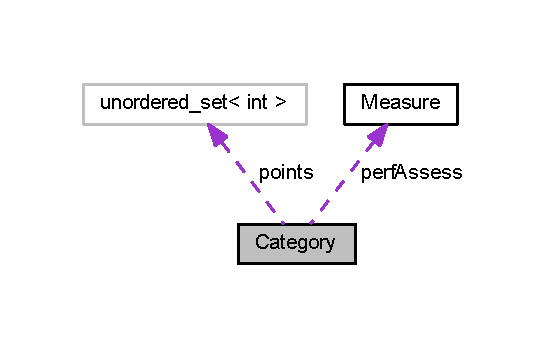
\includegraphics[width=263pt]{class_category__coll__graph}
\end{center}
\end{figure}
\subsection*{Public Member Functions}
\begin{DoxyCompactItemize}
\item 
\hyperlink{class_category_adeee911f773db1ebeb1005a00da45e08}{Category} ()
\item 
\hyperlink{class_category_aff8390ac4bbbf06c85648f76b78680d2}{Category} (int \hyperlink{class_category_a10f4f758d6942ef39ca6d1cc5dfb6369}{identifier}, std\+::string \&\hyperlink{class_category_a433491cdb802174ee504a41eea7bc7c7}{name})
\item 
void \hyperlink{class_category_a30dcc955d24ac3a6cfd2b37adbac5e14}{add\+Point} (int idx)
\item 
void \hyperlink{class_category_a213b1e03615488e5ef9ddd6189f8dc16}{remove\+Point} (int idx)
\item 
void \hyperlink{class_category_ad1816cec49d0c93cdc394f3c9292ecbb}{get\+Points} (std\+::vector$<$ int $>$ \&points\+Idx) const
\item 
std\+::string \hyperlink{class_category_a22e764bdb9b0d8d342c2971a1951a818}{to\+String} () const
\item 
const std\+::string \& \hyperlink{class_category_a23af5ca47bddcf85828a835ae188ed1f}{get\+Name} ()
\item 
const int \hyperlink{class_category_aad52cad1dde01976b9ee2fba33fb3661}{get\+Identifier} () const
\item 
unordered\+\_\+set$<$ int $>$ \& \hyperlink{class_category_af7bf3e19fc53d93b8c0d88974a03227c}{get\+Points} ()
\item 
\hyperlink{class_measure}{Measure} \& \hyperlink{class_category_a4752e892d1b8b078bfd4d9e1c13f8082}{get\+Perf\+Measure} ()
\item 
void \hyperlink{class_category_afb7ad18835edec07acf3c6129204f63d}{add\+TP} ()
\item 
void \hyperlink{class_category_a8ed7b1ffad6f82547b8d1fd68a1926f7}{add\+FP} ()
\item 
void \hyperlink{class_category_a6211d9ab0c6e542ce8ad675f7f51472f}{add\+FN} ()
\item 
double \hyperlink{class_category_aba83338fa764aa9d9157de0f2c24b07f}{precision} ()
\item 
double \hyperlink{class_category_a778001a2865033dbfb99fcc136815295}{recall} ()
\end{DoxyCompactItemize}
\subsection*{Protected Attributes}
\begin{DoxyCompactItemize}
\item 
int \hyperlink{class_category_a10f4f758d6942ef39ca6d1cc5dfb6369}{identifier}
\item 
std\+::string \hyperlink{class_category_a433491cdb802174ee504a41eea7bc7c7}{name}
\item 
unordered\+\_\+set$<$ int $>$ \hyperlink{class_category_a9b83a3525cbe3c9e806ca10f7c39f51f}{points}
\item 
\hyperlink{class_measure}{Measure} \hyperlink{class_category_ae2153cae8cf1b7eded7625a40e45ab8c}{perf\+Assess}
\end{DoxyCompactItemize}


\subsection{Detailed Description}
Represents an object category, e.\+g., apple, bowl, bell-\/pepper, etc. 

Open issues\+:
\begin{DoxyItemize}
\item a category should hold/handle its\textquotesingle{} own histogram. In this version the category\textquotesingle{} histogram is computed every time a new view-\/category prediction is made. A better approach could hold and maintain the histogram instead of computing it every time. 
\end{DoxyItemize}

Definition at line 28 of file Category.\+h.



\subsection{Constructor \& Destructor Documentation}
\mbox{\Hypertarget{class_category_adeee911f773db1ebeb1005a00da45e08}\label{class_category_adeee911f773db1ebeb1005a00da45e08}} 
\index{Category@{Category}!Category@{Category}}
\index{Category@{Category}!Category@{Category}}
\subsubsection{\texorpdfstring{Category()}{Category()}\hspace{0.1cm}{\footnotesize\ttfamily [1/2]}}
{\footnotesize\ttfamily Category\+::\+Category (\begin{DoxyParamCaption}{ }\end{DoxyParamCaption})}

The empty constructor is required when used as the value in a map. However! a call to this constructor could be due to an error so calling this constructor is considered a severe error and it is treated with an exception! No \char`\"{}not well formed object\char`\"{} are allowed to be injected into the applications\textquotesingle{} stream! 

Definition at line 5 of file Category.\+cpp.

\mbox{\Hypertarget{class_category_aff8390ac4bbbf06c85648f76b78680d2}\label{class_category_aff8390ac4bbbf06c85648f76b78680d2}} 
\index{Category@{Category}!Category@{Category}}
\index{Category@{Category}!Category@{Category}}
\subsubsection{\texorpdfstring{Category()}{Category()}\hspace{0.1cm}{\footnotesize\ttfamily [2/2]}}
{\footnotesize\ttfamily Category\+::\+Category (\begin{DoxyParamCaption}\item[{int}]{identifier,  }\item[{std\+::string \&}]{name }\end{DoxyParamCaption})}

Creates a new category.


\begin{DoxyParams}[1]{Parameters}
\mbox{\tt in}  & {\em identifier} & the unique identifier of the category \\
\hline
\mbox{\tt in}  & {\em name} & the name of the category, e.\+g., apple, tomato, etc. \\
\hline
\end{DoxyParams}


\subsection{Member Function Documentation}
\mbox{\Hypertarget{class_category_a6211d9ab0c6e542ce8ad675f7f51472f}\label{class_category_a6211d9ab0c6e542ce8ad675f7f51472f}} 
\index{Category@{Category}!add\+FN@{add\+FN}}
\index{add\+FN@{add\+FN}!Category@{Category}}
\subsubsection{\texorpdfstring{add\+F\+N()}{addFN()}}
{\footnotesize\ttfamily void Category\+::add\+FN (\begin{DoxyParamCaption}{ }\end{DoxyParamCaption})\hspace{0.3cm}{\ttfamily [inline]}}

Increments false negatives. 

Definition at line 140 of file Category.\+h.

\mbox{\Hypertarget{class_category_a8ed7b1ffad6f82547b8d1fd68a1926f7}\label{class_category_a8ed7b1ffad6f82547b8d1fd68a1926f7}} 
\index{Category@{Category}!add\+FP@{add\+FP}}
\index{add\+FP@{add\+FP}!Category@{Category}}
\subsubsection{\texorpdfstring{add\+F\+P()}{addFP()}}
{\footnotesize\ttfamily void Category\+::add\+FP (\begin{DoxyParamCaption}{ }\end{DoxyParamCaption})\hspace{0.3cm}{\ttfamily [inline]}}

Increments false positives. 

Definition at line 134 of file Category.\+h.

\mbox{\Hypertarget{class_category_a30dcc955d24ac3a6cfd2b37adbac5e14}\label{class_category_a30dcc955d24ac3a6cfd2b37adbac5e14}} 
\index{Category@{Category}!add\+Point@{add\+Point}}
\index{add\+Point@{add\+Point}!Category@{Category}}
\subsubsection{\texorpdfstring{add\+Point()}{addPoint()}}
{\footnotesize\ttfamily void Category\+::add\+Point (\begin{DoxyParamCaption}\item[{int}]{idx }\end{DoxyParamCaption})}

Adds a feature to the category.


\begin{DoxyParams}[1]{Parameters}
\mbox{\tt in}  & {\em idx} & the id of the feature to add (features\textquotesingle{} id in the main memory structure). \\
\hline
\end{DoxyParams}


Definition at line 32 of file Category.\+cpp.

\mbox{\Hypertarget{class_category_afb7ad18835edec07acf3c6129204f63d}\label{class_category_afb7ad18835edec07acf3c6129204f63d}} 
\index{Category@{Category}!add\+TP@{add\+TP}}
\index{add\+TP@{add\+TP}!Category@{Category}}
\subsubsection{\texorpdfstring{add\+T\+P()}{addTP()}}
{\footnotesize\ttfamily void Category\+::add\+TP (\begin{DoxyParamCaption}{ }\end{DoxyParamCaption})\hspace{0.3cm}{\ttfamily [inline]}}

Increments true positives. 

Definition at line 127 of file Category.\+h.

\mbox{\Hypertarget{class_category_aad52cad1dde01976b9ee2fba33fb3661}\label{class_category_aad52cad1dde01976b9ee2fba33fb3661}} 
\index{Category@{Category}!get\+Identifier@{get\+Identifier}}
\index{get\+Identifier@{get\+Identifier}!Category@{Category}}
\subsubsection{\texorpdfstring{get\+Identifier()}{getIdentifier()}}
{\footnotesize\ttfamily const int Category\+::get\+Identifier (\begin{DoxyParamCaption}{ }\end{DoxyParamCaption}) const\hspace{0.3cm}{\ttfamily [inline]}}

Gets the category identifier.

Issues\+: Is this identifier realy needed? It is the same as the map key in the main memory! T\+O\+DO\+: remove this? 

Definition at line 103 of file Category.\+h.

\mbox{\Hypertarget{class_category_a23af5ca47bddcf85828a835ae188ed1f}\label{class_category_a23af5ca47bddcf85828a835ae188ed1f}} 
\index{Category@{Category}!get\+Name@{get\+Name}}
\index{get\+Name@{get\+Name}!Category@{Category}}
\subsubsection{\texorpdfstring{get\+Name()}{getName()}}
{\footnotesize\ttfamily const std\+::string\& Category\+::get\+Name (\begin{DoxyParamCaption}{ }\end{DoxyParamCaption})\hspace{0.3cm}{\ttfamily [inline]}}

Gets the name of the category. 

Definition at line 92 of file Category.\+h.

\mbox{\Hypertarget{class_category_a4752e892d1b8b078bfd4d9e1c13f8082}\label{class_category_a4752e892d1b8b078bfd4d9e1c13f8082}} 
\index{Category@{Category}!get\+Perf\+Measure@{get\+Perf\+Measure}}
\index{get\+Perf\+Measure@{get\+Perf\+Measure}!Category@{Category}}
\subsubsection{\texorpdfstring{get\+Perf\+Measure()}{getPerfMeasure()}}
{\footnotesize\ttfamily \hyperlink{class_measure}{Measure}\& Category\+::get\+Perf\+Measure (\begin{DoxyParamCaption}{ }\end{DoxyParamCaption})\hspace{0.3cm}{\ttfamily [inline]}}

Gets the \hyperlink{class_measure}{Measure} class with information about the test results obtained for the category. 

Definition at line 120 of file Category.\+h.

\mbox{\Hypertarget{class_category_ad1816cec49d0c93cdc394f3c9292ecbb}\label{class_category_ad1816cec49d0c93cdc394f3c9292ecbb}} 
\index{Category@{Category}!get\+Points@{get\+Points}}
\index{get\+Points@{get\+Points}!Category@{Category}}
\subsubsection{\texorpdfstring{get\+Points()}{getPoints()}\hspace{0.1cm}{\footnotesize\ttfamily [1/2]}}
{\footnotesize\ttfamily void Category\+::get\+Points (\begin{DoxyParamCaption}\item[{std\+::vector$<$ int $>$ \&}]{points\+Idx }\end{DoxyParamCaption}) const}

Gets the features assigned to the category, i.\+e., the indeces of the features in main memory.

This is a read only method and it is probably not even used. T\+O\+DO\+: remove this method?


\begin{DoxyParams}[1]{Parameters}
\mbox{\tt out}  & {\em points\+Idx} & a vector holding the indeces (map keys) of the features assigned to the category. \\
\hline
\end{DoxyParams}
\mbox{\Hypertarget{class_category_af7bf3e19fc53d93b8c0d88974a03227c}\label{class_category_af7bf3e19fc53d93b8c0d88974a03227c}} 
\index{Category@{Category}!get\+Points@{get\+Points}}
\index{get\+Points@{get\+Points}!Category@{Category}}
\subsubsection{\texorpdfstring{get\+Points()}{getPoints()}\hspace{0.1cm}{\footnotesize\ttfamily [2/2]}}
{\footnotesize\ttfamily unordered\+\_\+set$<$int$>$\& Category\+::get\+Points (\begin{DoxyParamCaption}{ }\end{DoxyParamCaption})\hspace{0.3cm}{\ttfamily [inline]}}

Gets the feature indeces assigned to the category. 

Definition at line 110 of file Category.\+h.

\mbox{\Hypertarget{class_category_aba83338fa764aa9d9157de0f2c24b07f}\label{class_category_aba83338fa764aa9d9157de0f2c24b07f}} 
\index{Category@{Category}!precision@{precision}}
\index{precision@{precision}!Category@{Category}}
\subsubsection{\texorpdfstring{precision()}{precision()}}
{\footnotesize\ttfamily double Category\+::precision (\begin{DoxyParamCaption}{ }\end{DoxyParamCaption})\hspace{0.3cm}{\ttfamily [inline]}}

Gets the test precision value for the category. 

Definition at line 147 of file Category.\+h.

\mbox{\Hypertarget{class_category_a778001a2865033dbfb99fcc136815295}\label{class_category_a778001a2865033dbfb99fcc136815295}} 
\index{Category@{Category}!recall@{recall}}
\index{recall@{recall}!Category@{Category}}
\subsubsection{\texorpdfstring{recall()}{recall()}}
{\footnotesize\ttfamily double Category\+::recall (\begin{DoxyParamCaption}{ }\end{DoxyParamCaption})\hspace{0.3cm}{\ttfamily [inline]}}

Gets the test recall value for the category. 

Definition at line 154 of file Category.\+h.

\mbox{\Hypertarget{class_category_a213b1e03615488e5ef9ddd6189f8dc16}\label{class_category_a213b1e03615488e5ef9ddd6189f8dc16}} 
\index{Category@{Category}!remove\+Point@{remove\+Point}}
\index{remove\+Point@{remove\+Point}!Category@{Category}}
\subsubsection{\texorpdfstring{remove\+Point()}{removePoint()}}
{\footnotesize\ttfamily void Category\+::remove\+Point (\begin{DoxyParamCaption}\item[{int}]{idx }\end{DoxyParamCaption})}

Removes a feature from the category. Note\+: The feature is not removed from the main memory!


\begin{DoxyParams}[1]{Parameters}
\mbox{\tt in}  & {\em idx} & the id of the feature to remove (features\textquotesingle{} id in the main memory structure). \\
\hline
\end{DoxyParams}


Definition at line 37 of file Category.\+cpp.

\mbox{\Hypertarget{class_category_a22e764bdb9b0d8d342c2971a1951a818}\label{class_category_a22e764bdb9b0d8d342c2971a1951a818}} 
\index{Category@{Category}!to\+String@{to\+String}}
\index{to\+String@{to\+String}!Category@{Category}}
\subsubsection{\texorpdfstring{to\+String()}{toString()}}
{\footnotesize\ttfamily std\+::string Category\+::to\+String (\begin{DoxyParamCaption}{ }\end{DoxyParamCaption}) const}

A string representation, of the category, of the form\+: category\+\_\+name Id\+: category\+\_\+id P\+: unordered\+\_\+list\+\_\+of\+\_\+point\+\_\+ids

ex\+: apple Id\+: 1 P\+: 10, 12, 5, ...,

Notes\+: Used for debug purposes. 

Definition at line 14 of file Category.\+cpp.



\subsection{Member Data Documentation}
\mbox{\Hypertarget{class_category_a10f4f758d6942ef39ca6d1cc5dfb6369}\label{class_category_a10f4f758d6942ef39ca6d1cc5dfb6369}} 
\index{Category@{Category}!identifier@{identifier}}
\index{identifier@{identifier}!Category@{Category}}
\subsubsection{\texorpdfstring{identifier}{identifier}}
{\footnotesize\ttfamily int Category\+::identifier\hspace{0.3cm}{\ttfamily [protected]}}

The category unique identifier. 

Definition at line 162 of file Category.\+h.

\mbox{\Hypertarget{class_category_a433491cdb802174ee504a41eea7bc7c7}\label{class_category_a433491cdb802174ee504a41eea7bc7c7}} 
\index{Category@{Category}!name@{name}}
\index{name@{name}!Category@{Category}}
\subsubsection{\texorpdfstring{name}{name}}
{\footnotesize\ttfamily std\+::string Category\+::name\hspace{0.3cm}{\ttfamily [protected]}}

The category name. 

Definition at line 167 of file Category.\+h.

\mbox{\Hypertarget{class_category_ae2153cae8cf1b7eded7625a40e45ab8c}\label{class_category_ae2153cae8cf1b7eded7625a40e45ab8c}} 
\index{Category@{Category}!perf\+Assess@{perf\+Assess}}
\index{perf\+Assess@{perf\+Assess}!Category@{Category}}
\subsubsection{\texorpdfstring{perf\+Assess}{perfAssess}}
{\footnotesize\ttfamily \hyperlink{class_measure}{Measure} Category\+::perf\+Assess\hspace{0.3cm}{\ttfamily [protected]}}

Holds the recognition performance measures for the category. 

Definition at line 177 of file Category.\+h.

\mbox{\Hypertarget{class_category_a9b83a3525cbe3c9e806ca10f7c39f51f}\label{class_category_a9b83a3525cbe3c9e806ca10f7c39f51f}} 
\index{Category@{Category}!points@{points}}
\index{points@{points}!Category@{Category}}
\subsubsection{\texorpdfstring{points}{points}}
{\footnotesize\ttfamily unordered\+\_\+set$<$int$>$ Category\+::points\hspace{0.3cm}{\ttfamily [protected]}}

The features\textquotesingle{} ids assigned to the category (the map keys of the features in main memory). 

Definition at line 172 of file Category.\+h.



The documentation for this class was generated from the following files\+:\begin{DoxyCompactItemize}
\item 
H\+:/\+M\+E\+I/sistemas inteligentes/tp2/\+S\+I\+\_\+\+C\+O\+D\+E/include/\hyperlink{_category_8h}{Category.\+h}\item 
H\+:/\+M\+E\+I/sistemas inteligentes/tp2/\+S\+I\+\_\+\+C\+O\+D\+E/src/\hyperlink{_category_8cpp}{Category.\+cpp}\end{DoxyCompactItemize}

\hypertarget{class_category_recognizer}{}\section{Category\+Recognizer Class Reference}
\label{class_category_recognizer}\index{Category\+Recognizer@{Category\+Recognizer}}


This class assigns an object view to a category, based on the euclidean distance between the object view histogram and the categories histgrams.  




{\ttfamily \#include $<$Category\+Recognizer.\+h$>$}

\subsection*{Public Member Functions}
\begin{DoxyCompactItemize}
\item 
\hyperlink{class_category_recognizer_a67c56c30b0cb2783842c53169e7176c4}{Category\+Recognizer} (\hyperlink{class_memory}{Memory} \&memory, bool debug\+Mode=false)
\item 
\hyperlink{class_category_recognizer_a0b47f145ff89da44fa5191a52a6c558a}{$\sim$\+Category\+Recognizer} ()
\item 
void \hyperlink{class_category_recognizer_abb06a33eac9f693dc38a40f8c0b107f8}{assign\+View\+To\+Category} (std\+::vector$<$ int $>$ \&feats\+Idx, int category\+Id)
\item 
std\+::vector$<$ double $>$ $\ast$ \hyperlink{class_category_recognizer_ac712455609c64f0caca9977519824d7d}{get\+View\+Histogram} (std\+::vector$<$ int $>$ \&feats\+Idx, std\+::vector$<$ int $>$ \&redundancy\+Feats\+Idx)
\item 
std\+::vector$<$ double $>$ $\ast$ \hyperlink{class_category_recognizer_a9d9a2d29796bfd033a5045411392b195}{get\+View\+Histogram} (std\+::vector$<$ int $>$ \&feats\+Idx)
\item 
int \hyperlink{class_category_recognizer_ab66fab9c9404447350f1ce81adc83007}{get\+View\+Category} (std\+::vector$<$ double $>$ \&view\+Histogram)
\end{DoxyCompactItemize}


\subsection{Detailed Description}
This class assigns an object view to a category, based on the euclidean distance between the object view histogram and the categories histgrams. 

Histograms are vectors in N dimensions, N = number of clusters. Histograms are computed based on the features\textquotesingle{} local weight, i.\+e., its\textquotesingle{} category weight. Histograms are normalized using\+: sqrt(sum(\+Wli $\ast$ Wli)) $\vert$ Wli is the sum of the local wieghts of all features that belong to the view$\vert$category and to cluster i i = 1,..., N, N = number of clusters. 

Definition at line 36 of file Category\+Recognizer.\+h.



\subsection{Constructor \& Destructor Documentation}
\mbox{\Hypertarget{class_category_recognizer_a67c56c30b0cb2783842c53169e7176c4}\label{class_category_recognizer_a67c56c30b0cb2783842c53169e7176c4}} 
\index{Category\+Recognizer@{Category\+Recognizer}!Category\+Recognizer@{Category\+Recognizer}}
\index{Category\+Recognizer@{Category\+Recognizer}!Category\+Recognizer@{Category\+Recognizer}}
\subsubsection{\texorpdfstring{Category\+Recognizer()}{CategoryRecognizer()}}
{\footnotesize\ttfamily Category\+Recognizer\+::\+Category\+Recognizer (\begin{DoxyParamCaption}\item[{\hyperlink{class_memory}{Memory} \&}]{memory,  }\item[{bool}]{debug\+Mode = {\ttfamily false} }\end{DoxyParamCaption})}

Creates a new \hyperlink{class_category_recognizer}{Category\+Recognizer} class.


\begin{DoxyParams}[1]{Parameters}
\mbox{\tt in}  & {\em memory} & reference to the applications\textquotesingle{} memory structure. \\
\hline
\end{DoxyParams}


Definition at line 8 of file Category\+Recognizer.\+cpp.

\mbox{\Hypertarget{class_category_recognizer_a0b47f145ff89da44fa5191a52a6c558a}\label{class_category_recognizer_a0b47f145ff89da44fa5191a52a6c558a}} 
\index{Category\+Recognizer@{Category\+Recognizer}!````~Category\+Recognizer@{$\sim$\+Category\+Recognizer}}
\index{````~Category\+Recognizer@{$\sim$\+Category\+Recognizer}!Category\+Recognizer@{Category\+Recognizer}}
\subsubsection{\texorpdfstring{$\sim$\+Category\+Recognizer()}{~CategoryRecognizer()}}
{\footnotesize\ttfamily Category\+Recognizer\+::$\sim$\+Category\+Recognizer (\begin{DoxyParamCaption}{ }\end{DoxyParamCaption})}



Definition at line 12 of file Category\+Recognizer.\+cpp.



\subsection{Member Function Documentation}
\mbox{\Hypertarget{class_category_recognizer_abb06a33eac9f693dc38a40f8c0b107f8}\label{class_category_recognizer_abb06a33eac9f693dc38a40f8c0b107f8}} 
\index{Category\+Recognizer@{Category\+Recognizer}!assign\+View\+To\+Category@{assign\+View\+To\+Category}}
\index{assign\+View\+To\+Category@{assign\+View\+To\+Category}!Category\+Recognizer@{Category\+Recognizer}}
\subsubsection{\texorpdfstring{assign\+View\+To\+Category()}{assignViewToCategory()}}
{\footnotesize\ttfamily void Category\+Recognizer\+::assign\+View\+To\+Category (\begin{DoxyParamCaption}\item[{std\+::vector$<$ int $>$ \&}]{feats\+Idx,  }\item[{int}]{category\+Id }\end{DoxyParamCaption})}

Assigns every feature of a given object view to the given category id.


\begin{DoxyParams}[1]{Parameters}
\mbox{\tt in}  & {\em feats\+Idx} & the objects\textquotesingle{} view feature indeces to assign. \\
\hline
\mbox{\tt in}  & {\em category\+Id} & the category id to assign the features to. \\
\hline
\end{DoxyParams}


Definition at line 212 of file Category\+Recognizer.\+cpp.

\mbox{\Hypertarget{class_category_recognizer_ab66fab9c9404447350f1ce81adc83007}\label{class_category_recognizer_ab66fab9c9404447350f1ce81adc83007}} 
\index{Category\+Recognizer@{Category\+Recognizer}!get\+View\+Category@{get\+View\+Category}}
\index{get\+View\+Category@{get\+View\+Category}!Category\+Recognizer@{Category\+Recognizer}}
\subsubsection{\texorpdfstring{get\+View\+Category()}{getViewCategory()}}
{\footnotesize\ttfamily int Category\+Recognizer\+::get\+View\+Category (\begin{DoxyParamCaption}\item[{std\+::vector$<$ double $>$ \&}]{view\+Histogram }\end{DoxyParamCaption})}

Assigns a view to a category based on the view and category histograms. The histograms are normalized!

Open issues\+: the categories\textquotesingle{}s histograms are computed every time.


\begin{DoxyParams}[1]{Parameters}
\mbox{\tt in}  & {\em view\+Histogram} & the objects\textquotesingle{} view histogram \\
\hline
\mbox{\tt out}  & {\em returns} & the object view predicted category id. \\
\hline
\end{DoxyParams}


Definition at line 132 of file Category\+Recognizer.\+cpp.

\mbox{\Hypertarget{class_category_recognizer_ac712455609c64f0caca9977519824d7d}\label{class_category_recognizer_ac712455609c64f0caca9977519824d7d}} 
\index{Category\+Recognizer@{Category\+Recognizer}!get\+View\+Histogram@{get\+View\+Histogram}}
\index{get\+View\+Histogram@{get\+View\+Histogram}!Category\+Recognizer@{Category\+Recognizer}}
\subsubsection{\texorpdfstring{get\+View\+Histogram()}{getViewHistogram()}\hspace{0.1cm}{\footnotesize\ttfamily [1/2]}}
{\footnotesize\ttfamily std\+::vector$<$double$>$$\ast$ Category\+Recognizer\+::get\+View\+Histogram (\begin{DoxyParamCaption}\item[{std\+::vector$<$ int $>$ \&}]{feats\+Idx,  }\item[{std\+::vector$<$ int $>$ \&}]{redundancy\+Feats\+Idx }\end{DoxyParamCaption})}

Computes the objects\textquotesingle{} view histogram.


\begin{DoxyParams}[1]{Parameters}
\mbox{\tt in}  & {\em feats\+Idx} & the objects\textquotesingle{} view feature indices seen for the first time. \\
\hline
\mbox{\tt in}  & {\em redundancy\+Feats\+Idx} & the objects\textquotesingle{} view feature indeces of features already in memory (redundancy). replacing seen redundant features\\
\hline
\mbox{\tt out}  & {\em returns} & the view histogram as a vector in N dimensions, where N is the number of clusters. \\
\hline
\end{DoxyParams}
\mbox{\Hypertarget{class_category_recognizer_a9d9a2d29796bfd033a5045411392b195}\label{class_category_recognizer_a9d9a2d29796bfd033a5045411392b195}} 
\index{Category\+Recognizer@{Category\+Recognizer}!get\+View\+Histogram@{get\+View\+Histogram}}
\index{get\+View\+Histogram@{get\+View\+Histogram}!Category\+Recognizer@{Category\+Recognizer}}
\subsubsection{\texorpdfstring{get\+View\+Histogram()}{getViewHistogram()}\hspace{0.1cm}{\footnotesize\ttfamily [2/2]}}
{\footnotesize\ttfamily std\+::vector$<$ double $>$ $\ast$ Category\+Recognizer\+::get\+View\+Histogram (\begin{DoxyParamCaption}\item[{std\+::vector$<$ int $>$ \&}]{feats\+Idx }\end{DoxyParamCaption})}

Computes the objects\textquotesingle{} view histogram.


\begin{DoxyParams}[1]{Parameters}
\mbox{\tt in}  & {\em feats\+Idx} & the objects\textquotesingle{} view features indices seen for the first time.\\
\hline
\mbox{\tt out}  & {\em returns} & the view histogram as a vector in N dimensions, where N is the number of clusters. \\
\hline
\end{DoxyParams}


Definition at line 80 of file Category\+Recognizer.\+cpp.



The documentation for this class was generated from the following files\+:\begin{DoxyCompactItemize}
\item 
H\+:/\+M\+E\+I/sistemas inteligentes/tp2/\+S\+I\+\_\+\+C\+O\+D\+E/include/\hyperlink{_category_recognizer_8h}{Category\+Recognizer.\+h}\item 
H\+:/\+M\+E\+I/sistemas inteligentes/tp2/\+S\+I\+\_\+\+C\+O\+D\+E/src/\hyperlink{_category_recognizer_8cpp}{Category\+Recognizer.\+cpp}\end{DoxyCompactItemize}

\hypertarget{struct_memory_1_1_category_view_distance}{}\section{Memory\+:\+:Category\+View\+Distance Struct Reference}
\label{struct_memory_1_1_category_view_distance}\index{Memory\+::\+Category\+View\+Distance@{Memory\+::\+Category\+View\+Distance}}


Auxiliar data structure to hold the distances between a specific object view and the categories. The distance is the euclidean distance between the respective histograms.  




{\ttfamily \#include $<$Memory.\+h$>$}

\subsection*{Public Member Functions}
\begin{DoxyCompactItemize}
\item 
\hyperlink{struct_memory_1_1_category_view_distance_a3e0c631eb136eb7a914d85f184cae552}{Category\+View\+Distance} (int \hyperlink{struct_memory_1_1_category_view_distance_aaa0114f6bc41b1df4cc5fb5f4eb11017}{category\+Id}, double \hyperlink{struct_memory_1_1_category_view_distance_aab4f1397e33f96a80d6e5e77cc66593c}{distance})
\item 
bool \hyperlink{struct_memory_1_1_category_view_distance_afa1664995bbdebd301f7f5ee33aa9c0e}{operator$<$} (const \hyperlink{struct_memory_1_1_category_view_distance}{Category\+View\+Distance} \&o) const
\end{DoxyCompactItemize}
\subsection*{Public Attributes}
\begin{DoxyCompactItemize}
\item 
int \hyperlink{struct_memory_1_1_category_view_distance_aaa0114f6bc41b1df4cc5fb5f4eb11017}{category\+Id}
\item 
double \hyperlink{struct_memory_1_1_category_view_distance_aab4f1397e33f96a80d6e5e77cc66593c}{distance}
\end{DoxyCompactItemize}


\subsection{Detailed Description}
Auxiliar data structure to hold the distances between a specific object view and the categories. The distance is the euclidean distance between the respective histograms. 

Definition at line 698 of file Memory.\+h.



\subsection{Constructor \& Destructor Documentation}
\mbox{\Hypertarget{struct_memory_1_1_category_view_distance_a3e0c631eb136eb7a914d85f184cae552}\label{struct_memory_1_1_category_view_distance_a3e0c631eb136eb7a914d85f184cae552}} 
\index{Memory\+::\+Category\+View\+Distance@{Memory\+::\+Category\+View\+Distance}!Category\+View\+Distance@{Category\+View\+Distance}}
\index{Category\+View\+Distance@{Category\+View\+Distance}!Memory\+::\+Category\+View\+Distance@{Memory\+::\+Category\+View\+Distance}}
\subsubsection{\texorpdfstring{Category\+View\+Distance()}{CategoryViewDistance()}}
{\footnotesize\ttfamily Memory\+::\+Category\+View\+Distance\+::\+Category\+View\+Distance (\begin{DoxyParamCaption}\item[{int}]{category\+Id,  }\item[{double}]{distance }\end{DoxyParamCaption})\hspace{0.3cm}{\ttfamily [inline]}}



Definition at line 702 of file Memory.\+h.



\subsection{Member Function Documentation}
\mbox{\Hypertarget{struct_memory_1_1_category_view_distance_afa1664995bbdebd301f7f5ee33aa9c0e}\label{struct_memory_1_1_category_view_distance_afa1664995bbdebd301f7f5ee33aa9c0e}} 
\index{Memory\+::\+Category\+View\+Distance@{Memory\+::\+Category\+View\+Distance}!operator$<$@{operator$<$}}
\index{operator$<$@{operator$<$}!Memory\+::\+Category\+View\+Distance@{Memory\+::\+Category\+View\+Distance}}
\subsubsection{\texorpdfstring{operator$<$()}{operator<()}}
{\footnotesize\ttfamily bool Memory\+::\+Category\+View\+Distance\+::operator$<$ (\begin{DoxyParamCaption}\item[{const \hyperlink{struct_memory_1_1_category_view_distance}{Category\+View\+Distance} \&}]{o }\end{DoxyParamCaption}) const\hspace{0.3cm}{\ttfamily [inline]}}



Definition at line 705 of file Memory.\+h.



\subsection{Member Data Documentation}
\mbox{\Hypertarget{struct_memory_1_1_category_view_distance_aaa0114f6bc41b1df4cc5fb5f4eb11017}\label{struct_memory_1_1_category_view_distance_aaa0114f6bc41b1df4cc5fb5f4eb11017}} 
\index{Memory\+::\+Category\+View\+Distance@{Memory\+::\+Category\+View\+Distance}!category\+Id@{category\+Id}}
\index{category\+Id@{category\+Id}!Memory\+::\+Category\+View\+Distance@{Memory\+::\+Category\+View\+Distance}}
\subsubsection{\texorpdfstring{category\+Id}{categoryId}}
{\footnotesize\ttfamily int Memory\+::\+Category\+View\+Distance\+::category\+Id}



Definition at line 699 of file Memory.\+h.

\mbox{\Hypertarget{struct_memory_1_1_category_view_distance_aab4f1397e33f96a80d6e5e77cc66593c}\label{struct_memory_1_1_category_view_distance_aab4f1397e33f96a80d6e5e77cc66593c}} 
\index{Memory\+::\+Category\+View\+Distance@{Memory\+::\+Category\+View\+Distance}!distance@{distance}}
\index{distance@{distance}!Memory\+::\+Category\+View\+Distance@{Memory\+::\+Category\+View\+Distance}}
\subsubsection{\texorpdfstring{distance}{distance}}
{\footnotesize\ttfamily double Memory\+::\+Category\+View\+Distance\+::distance}



Definition at line 700 of file Memory.\+h.



The documentation for this struct was generated from the following file\+:\begin{DoxyCompactItemize}
\item 
H\+:/\+M\+E\+I/sistemas inteligentes/tp2/\+S\+I\+\_\+\+C\+O\+D\+E/include/\hyperlink{_memory_8h}{Memory.\+h}\end{DoxyCompactItemize}

\hypertarget{class_cluster}{}\section{Cluster Class Reference}
\label{class_cluster}\index{Cluster@{Cluster}}


Represents a cluster.  




{\ttfamily \#include $<$Cluster.\+h$>$}



Collaboration diagram for Cluster\+:
\nopagebreak
\begin{figure}[H]
\begin{center}
\leavevmode
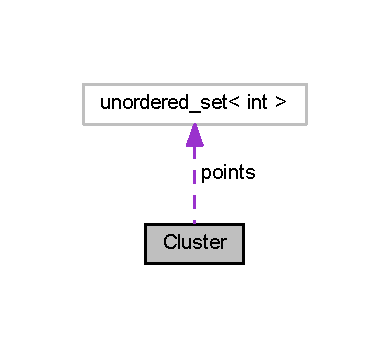
\includegraphics[width=187pt]{class_cluster__coll__graph}
\end{center}
\end{figure}
\subsection*{Public Member Functions}
\begin{DoxyCompactItemize}
\item 
\hyperlink{class_cluster_aee7feb1d599d4c8fda6c3ee83e86ba81}{Cluster} ()
\item 
\hyperlink{class_cluster_a7ec216455347ce05a9e0b410378a01f9}{Cluster} (int \hyperlink{class_cluster_a5b3de44acabe712cdcc405fa40f8812a}{identifier}, pcl\+::\+Histogram$<$ 153 $>$ \&center)
\item 
void \hyperlink{class_cluster_a9af018a96861327b211e6fe5c7290f52}{set\+Centroid} (pcl\+::\+Histogram$<$ 153 $>$ \&center)
\item 
void \hyperlink{class_cluster_af01610223d1a98628ba974609918db91}{add\+Point} (int \&idx)
\item 
void \hyperlink{class_cluster_aa0e0757d491b0b201500c64978abdaf8}{remove\+Point} (int \&idx)
\item 
void \hyperlink{class_cluster_a0c4f4cc4e9249ac54ccb995b7d027f52}{clear\+Points} ()
\item 
void \hyperlink{class_cluster_a77511825a9d51c343a20565a7e71a23c}{get\+Points} (std\+::vector$<$ int $>$ \&points\+Idx) const
\item 
const int \hyperlink{class_cluster_add3a7f58320774fdfcb3772b992115a0}{get\+Random\+Point} ()
\item 
const int \hyperlink{class_cluster_aab876ab329ebaa1c4baaac5bf5dadcbf}{get\+Random\+Point} (int \&point\+Idx)
\item 
float \& \hyperlink{class_cluster_a7b871b24968ca5c63bfd32cda9ff6c75}{add\+To\+Sum\+Weight} (const float \&weight)
\item 
float \& \hyperlink{class_cluster_a93b4f6092b558747d0882bf0af959da8}{subtract\+From\+Sum\+Weight} (const float \&weight)
\item 
pcl\+::\+Histogram$<$ 153 $>$ \& \hyperlink{class_cluster_ac0922c4c1a1d54fbd9971a77b785698d}{add\+To\+Sum\+Features} (pcl\+::\+Histogram$<$ 153 $>$ \&feat, const float \&feat\+Weight)
\item 
pcl\+::\+Histogram$<$ 153 $>$ \& \hyperlink{class_cluster_a8cf196c9c3f77aeeafb7b793967e17ed}{remove\+From\+Sum\+Features} (pcl\+::\+Histogram$<$ 153 $>$ \&feat, const float \&feat\+Weight)
\item 
void \hyperlink{class_cluster_a3ed40ce6adf7cc47b9e5721baed4fb51}{recompute\+Centroid} ()
\item 
void \hyperlink{class_cluster_ad164f4a4c7eb8d35b8098149d83246db}{reset\+Cluster\+Totals} ()
\item 
pcl\+::\+Histogram$<$ 153 $>$ \& \hyperlink{class_cluster_ad4e959d20fb0c9b208ee97e2082c51b1}{get\+Centroid} ()
\item 
const int \& \hyperlink{class_cluster_a78429c346e1fdfe24fbd3863a16c924f}{get\+Identifier} () const
\item 
unordered\+\_\+set$<$ int $>$ \& \hyperlink{class_cluster_a14344a9dd9efc93609344cc3fb018f37}{get\+Points} ()
\item 
int \hyperlink{class_cluster_a3de9ef447e04c6691a5010d3b0b7916b}{size} ()
\item 
float \& \hyperlink{class_cluster_ac011ee866632afed7b36759f9675f01f}{get\+Sum\+Weight} ()
\item 
void \hyperlink{class_cluster_a4cd75a1e9afb0d72b0d91c5549869ce1}{reset\+Sum\+Weight} ()
\item 
pcl\+::\+Histogram$<$ 153 $>$ \& \hyperlink{class_cluster_ab5d2cbdb6de3a6efbecaab959503714b}{get\+Sum\+Features} ()
\item 
void \hyperlink{class_cluster_a0ea9e78709352146e9a0f3bcb0574928}{reset\+Sum\+Features} ()
\item 
float \& \hyperlink{class_cluster_ab8c35f60eff5f2f4c0508900650b058c}{get\+Wss} ()
\item 
void \hyperlink{class_cluster_a400d6e1f3b7e206bec4821dcf5aef3ec}{set\+Wss} (float \&val)
\item 
float \& \hyperlink{class_cluster_acc50770cbc475efa285a2ff79b335530}{get\+Bss} ()
\item 
void \hyperlink{class_cluster_a6d4da0772bd78a707e59d90a4a026588}{set\+Bss} (float \&val)
\end{DoxyCompactItemize}
\subsection*{Protected Attributes}
\begin{DoxyCompactItemize}
\item 
int \hyperlink{class_cluster_a5b3de44acabe712cdcc405fa40f8812a}{identifier}
\item 
pcl\+::\+Histogram$<$ 153 $>$ \hyperlink{class_cluster_a06b612a067c349bd2a56d1960d229e2a}{centroid}
\item 
unordered\+\_\+set$<$ int $>$ \hyperlink{class_cluster_a9aa583a643474a3744e1508ab51807d5}{points}
\item 
float \hyperlink{class_cluster_a1380f8914d5f22ca56afe13dd323d8e5}{sum\+Weight}
\item 
pcl\+::\+Histogram$<$ 153 $>$ \hyperlink{class_cluster_a9440083a17c6144a556433afa719e8ad}{sum\+Features}
\item 
float \hyperlink{class_cluster_a3485a5dc53d0094f618b9308aea59288}{wss}
\item 
float \hyperlink{class_cluster_aa83d01b4c4d33763154c82cbfdce7fff}{bss}
\end{DoxyCompactItemize}


\subsection{Detailed Description}
Represents a cluster. 

Definition at line 17 of file Cluster.\+h.



\subsection{Constructor \& Destructor Documentation}
\mbox{\Hypertarget{class_cluster_aee7feb1d599d4c8fda6c3ee83e86ba81}\label{class_cluster_aee7feb1d599d4c8fda6c3ee83e86ba81}} 
\index{Cluster@{Cluster}!Cluster@{Cluster}}
\index{Cluster@{Cluster}!Cluster@{Cluster}}
\subsubsection{\texorpdfstring{Cluster()}{Cluster()}\hspace{0.1cm}{\footnotesize\ttfamily [1/2]}}
{\footnotesize\ttfamily Cluster\+::\+Cluster (\begin{DoxyParamCaption}{ }\end{DoxyParamCaption})\hspace{0.3cm}{\ttfamily [inline]}}

The empty constructor is required when used as the value in a map. However calling it is considered an error since an invalid object will be injected into the system! 

Definition at line 24 of file Cluster.\+h.

\mbox{\Hypertarget{class_cluster_a7ec216455347ce05a9e0b410378a01f9}\label{class_cluster_a7ec216455347ce05a9e0b410378a01f9}} 
\index{Cluster@{Cluster}!Cluster@{Cluster}}
\index{Cluster@{Cluster}!Cluster@{Cluster}}
\subsubsection{\texorpdfstring{Cluster()}{Cluster()}\hspace{0.1cm}{\footnotesize\ttfamily [2/2]}}
{\footnotesize\ttfamily Cluster\+::\+Cluster (\begin{DoxyParamCaption}\item[{int}]{identifier,  }\item[{pcl\+::\+Histogram$<$ 153 $>$ \&}]{center }\end{DoxyParamCaption})}


\begin{DoxyParams}[1]{Parameters}
\mbox{\tt in}  & {\em identifier} & the unique identifier of the cluster \\
\hline
\mbox{\tt in}  & {\em center} & the centroid of the cluster \\
\hline
\end{DoxyParams}


\subsection{Member Function Documentation}
\mbox{\Hypertarget{class_cluster_af01610223d1a98628ba974609918db91}\label{class_cluster_af01610223d1a98628ba974609918db91}} 
\index{Cluster@{Cluster}!add\+Point@{add\+Point}}
\index{add\+Point@{add\+Point}!Cluster@{Cluster}}
\subsubsection{\texorpdfstring{add\+Point()}{addPoint()}}
{\footnotesize\ttfamily void Cluster\+::add\+Point (\begin{DoxyParamCaption}\item[{int \&}]{idx }\end{DoxyParamCaption})}

Adds a feature to the cluster (the index of the feature in main memory is used). 
\begin{DoxyParams}[1]{Parameters}
\mbox{\tt in}  & {\em idx} & the index of the feature in the main memory structure dictionary (its key). \\
\hline
\end{DoxyParams}


Definition at line 19 of file Cluster.\+cpp.

\mbox{\Hypertarget{class_cluster_ac0922c4c1a1d54fbd9971a77b785698d}\label{class_cluster_ac0922c4c1a1d54fbd9971a77b785698d}} 
\index{Cluster@{Cluster}!add\+To\+Sum\+Features@{add\+To\+Sum\+Features}}
\index{add\+To\+Sum\+Features@{add\+To\+Sum\+Features}!Cluster@{Cluster}}
\subsubsection{\texorpdfstring{add\+To\+Sum\+Features()}{addToSumFeatures()}}
{\footnotesize\ttfamily Histogram$<$ 153 $>$ \& Cluster\+::add\+To\+Sum\+Features (\begin{DoxyParamCaption}\item[{pcl\+::\+Histogram$<$ 153 $>$ \&}]{feat,  }\item[{const float \&}]{feat\+Weight }\end{DoxyParamCaption})}

Adds the product (feat $\ast$ feat\+Weight) of a new feature to the running weighted sum of features


\begin{DoxyParams}[1]{Parameters}
\mbox{\tt in}  & {\em feat} & the feature \\
\hline
\mbox{\tt in}  & {\em feat\+Weight} & the global weight of the feature \\
\hline
\end{DoxyParams}


Definition at line 73 of file Cluster.\+cpp.

\mbox{\Hypertarget{class_cluster_a7b871b24968ca5c63bfd32cda9ff6c75}\label{class_cluster_a7b871b24968ca5c63bfd32cda9ff6c75}} 
\index{Cluster@{Cluster}!add\+To\+Sum\+Weight@{add\+To\+Sum\+Weight}}
\index{add\+To\+Sum\+Weight@{add\+To\+Sum\+Weight}!Cluster@{Cluster}}
\subsubsection{\texorpdfstring{add\+To\+Sum\+Weight()}{addToSumWeight()}}
{\footnotesize\ttfamily float \& Cluster\+::add\+To\+Sum\+Weight (\begin{DoxyParamCaption}\item[{const float \&}]{weight }\end{DoxyParamCaption})}

Adds a new weight to the running sum of weights


\begin{DoxyParams}[1]{Parameters}
\mbox{\tt in}  & {\em weight} & the new weight to add \\
\hline
\end{DoxyParams}


Definition at line 63 of file Cluster.\+cpp.

\mbox{\Hypertarget{class_cluster_a0c4f4cc4e9249ac54ccb995b7d027f52}\label{class_cluster_a0c4f4cc4e9249ac54ccb995b7d027f52}} 
\index{Cluster@{Cluster}!clear\+Points@{clear\+Points}}
\index{clear\+Points@{clear\+Points}!Cluster@{Cluster}}
\subsubsection{\texorpdfstring{clear\+Points()}{clearPoints()}}
{\footnotesize\ttfamily void Cluster\+::clear\+Points (\begin{DoxyParamCaption}{ }\end{DoxyParamCaption})}

Remove all points from the list of popints assigned to the cluster. 

Definition at line 27 of file Cluster.\+cpp.

\mbox{\Hypertarget{class_cluster_acc50770cbc475efa285a2ff79b335530}\label{class_cluster_acc50770cbc475efa285a2ff79b335530}} 
\index{Cluster@{Cluster}!get\+Bss@{get\+Bss}}
\index{get\+Bss@{get\+Bss}!Cluster@{Cluster}}
\subsubsection{\texorpdfstring{get\+Bss()}{getBss()}}
{\footnotesize\ttfamily float\& Cluster\+::get\+Bss (\begin{DoxyParamCaption}{ }\end{DoxyParamCaption})\hspace{0.3cm}{\ttfamily [inline]}}



Definition at line 221 of file Cluster.\+h.

\mbox{\Hypertarget{class_cluster_ad4e959d20fb0c9b208ee97e2082c51b1}\label{class_cluster_ad4e959d20fb0c9b208ee97e2082c51b1}} 
\index{Cluster@{Cluster}!get\+Centroid@{get\+Centroid}}
\index{get\+Centroid@{get\+Centroid}!Cluster@{Cluster}}
\subsubsection{\texorpdfstring{get\+Centroid()}{getCentroid()}}
{\footnotesize\ttfamily pcl\+::\+Histogram$<$153$>$\& Cluster\+::get\+Centroid (\begin{DoxyParamCaption}{ }\end{DoxyParamCaption})\hspace{0.3cm}{\ttfamily [inline]}}



Definition at line 170 of file Cluster.\+h.

\mbox{\Hypertarget{class_cluster_a78429c346e1fdfe24fbd3863a16c924f}\label{class_cluster_a78429c346e1fdfe24fbd3863a16c924f}} 
\index{Cluster@{Cluster}!get\+Identifier@{get\+Identifier}}
\index{get\+Identifier@{get\+Identifier}!Cluster@{Cluster}}
\subsubsection{\texorpdfstring{get\+Identifier()}{getIdentifier()}}
{\footnotesize\ttfamily const int\& Cluster\+::get\+Identifier (\begin{DoxyParamCaption}{ }\end{DoxyParamCaption}) const\hspace{0.3cm}{\ttfamily [inline]}}



Definition at line 174 of file Cluster.\+h.

\mbox{\Hypertarget{class_cluster_a77511825a9d51c343a20565a7e71a23c}\label{class_cluster_a77511825a9d51c343a20565a7e71a23c}} 
\index{Cluster@{Cluster}!get\+Points@{get\+Points}}
\index{get\+Points@{get\+Points}!Cluster@{Cluster}}
\subsubsection{\texorpdfstring{get\+Points()}{getPoints()}\hspace{0.1cm}{\footnotesize\ttfamily [1/2]}}
{\footnotesize\ttfamily void Cluster\+::get\+Points (\begin{DoxyParamCaption}\item[{std\+::vector$<$ int $>$ \&}]{points\+Idx }\end{DoxyParamCaption}) const}

Return the features assigned to the cluster (the indeces of the features in main memory are returned). 
\begin{DoxyParams}[1]{Parameters}
\mbox{\tt out}  & {\em points\+Idx} & a vector holding the indeces (map keys) of the features assigned to the cluster. \\
\hline
\end{DoxyParams}
\mbox{\Hypertarget{class_cluster_a14344a9dd9efc93609344cc3fb018f37}\label{class_cluster_a14344a9dd9efc93609344cc3fb018f37}} 
\index{Cluster@{Cluster}!get\+Points@{get\+Points}}
\index{get\+Points@{get\+Points}!Cluster@{Cluster}}
\subsubsection{\texorpdfstring{get\+Points()}{getPoints()}\hspace{0.1cm}{\footnotesize\ttfamily [2/2]}}
{\footnotesize\ttfamily unordered\+\_\+set$<$int$>$\& Cluster\+::get\+Points (\begin{DoxyParamCaption}{ }\end{DoxyParamCaption})\hspace{0.3cm}{\ttfamily [inline]}}



Definition at line 178 of file Cluster.\+h.

\mbox{\Hypertarget{class_cluster_add3a7f58320774fdfcb3772b992115a0}\label{class_cluster_add3a7f58320774fdfcb3772b992115a0}} 
\index{Cluster@{Cluster}!get\+Random\+Point@{get\+Random\+Point}}
\index{get\+Random\+Point@{get\+Random\+Point}!Cluster@{Cluster}}
\subsubsection{\texorpdfstring{get\+Random\+Point()}{getRandomPoint()}\hspace{0.1cm}{\footnotesize\ttfamily [1/2]}}
{\footnotesize\ttfamily const int Cluster\+::get\+Random\+Point (\begin{DoxyParamCaption}{ }\end{DoxyParamCaption})}

Get a random point index from the set of points in the cluster 

Definition at line 36 of file Cluster.\+cpp.

\mbox{\Hypertarget{class_cluster_aab876ab329ebaa1c4baaac5bf5dadcbf}\label{class_cluster_aab876ab329ebaa1c4baaac5bf5dadcbf}} 
\index{Cluster@{Cluster}!get\+Random\+Point@{get\+Random\+Point}}
\index{get\+Random\+Point@{get\+Random\+Point}!Cluster@{Cluster}}
\subsubsection{\texorpdfstring{get\+Random\+Point()}{getRandomPoint()}\hspace{0.1cm}{\footnotesize\ttfamily [2/2]}}
{\footnotesize\ttfamily const int Cluster\+::get\+Random\+Point (\begin{DoxyParamCaption}\item[{int \&}]{point\+Idx }\end{DoxyParamCaption})}

Get a random point index from the set of points in the cluster


\begin{DoxyParams}[1]{Parameters}
\mbox{\tt in}  & {\em point\+Idx} & the value not to duplicate\\
\hline
\end{DoxyParams}
Returns random number but different from the specified value 

Definition at line 51 of file Cluster.\+cpp.

\mbox{\Hypertarget{class_cluster_ab5d2cbdb6de3a6efbecaab959503714b}\label{class_cluster_ab5d2cbdb6de3a6efbecaab959503714b}} 
\index{Cluster@{Cluster}!get\+Sum\+Features@{get\+Sum\+Features}}
\index{get\+Sum\+Features@{get\+Sum\+Features}!Cluster@{Cluster}}
\subsubsection{\texorpdfstring{get\+Sum\+Features()}{getSumFeatures()}}
{\footnotesize\ttfamily pcl\+::\+Histogram$<$153$>$\& Cluster\+::get\+Sum\+Features (\begin{DoxyParamCaption}{ }\end{DoxyParamCaption})\hspace{0.3cm}{\ttfamily [inline]}}



Definition at line 203 of file Cluster.\+h.

\mbox{\Hypertarget{class_cluster_ac011ee866632afed7b36759f9675f01f}\label{class_cluster_ac011ee866632afed7b36759f9675f01f}} 
\index{Cluster@{Cluster}!get\+Sum\+Weight@{get\+Sum\+Weight}}
\index{get\+Sum\+Weight@{get\+Sum\+Weight}!Cluster@{Cluster}}
\subsubsection{\texorpdfstring{get\+Sum\+Weight()}{getSumWeight()}}
{\footnotesize\ttfamily float\& Cluster\+::get\+Sum\+Weight (\begin{DoxyParamCaption}{ }\end{DoxyParamCaption})\hspace{0.3cm}{\ttfamily [inline]}}



Definition at line 192 of file Cluster.\+h.

\mbox{\Hypertarget{class_cluster_ab8c35f60eff5f2f4c0508900650b058c}\label{class_cluster_ab8c35f60eff5f2f4c0508900650b058c}} 
\index{Cluster@{Cluster}!get\+Wss@{get\+Wss}}
\index{get\+Wss@{get\+Wss}!Cluster@{Cluster}}
\subsubsection{\texorpdfstring{get\+Wss()}{getWss()}}
{\footnotesize\ttfamily float\& Cluster\+::get\+Wss (\begin{DoxyParamCaption}{ }\end{DoxyParamCaption})\hspace{0.3cm}{\ttfamily [inline]}}



Definition at line 213 of file Cluster.\+h.

\mbox{\Hypertarget{class_cluster_a3ed40ce6adf7cc47b9e5721baed4fb51}\label{class_cluster_a3ed40ce6adf7cc47b9e5721baed4fb51}} 
\index{Cluster@{Cluster}!recompute\+Centroid@{recompute\+Centroid}}
\index{recompute\+Centroid@{recompute\+Centroid}!Cluster@{Cluster}}
\subsubsection{\texorpdfstring{recompute\+Centroid()}{recomputeCentroid()}}
{\footnotesize\ttfamily void Cluster\+::recompute\+Centroid (\begin{DoxyParamCaption}{ }\end{DoxyParamCaption})}

Recompute the cluster centroid based on the running sums (sum\+Features / sum\+Weight) 

Definition at line 87 of file Cluster.\+cpp.

\mbox{\Hypertarget{class_cluster_a8cf196c9c3f77aeeafb7b793967e17ed}\label{class_cluster_a8cf196c9c3f77aeeafb7b793967e17ed}} 
\index{Cluster@{Cluster}!remove\+From\+Sum\+Features@{remove\+From\+Sum\+Features}}
\index{remove\+From\+Sum\+Features@{remove\+From\+Sum\+Features}!Cluster@{Cluster}}
\subsubsection{\texorpdfstring{remove\+From\+Sum\+Features()}{removeFromSumFeatures()}}
{\footnotesize\ttfamily Histogram$<$ 153 $>$ \& Cluster\+::remove\+From\+Sum\+Features (\begin{DoxyParamCaption}\item[{pcl\+::\+Histogram$<$ 153 $>$ \&}]{feat,  }\item[{const float \&}]{feat\+Weight }\end{DoxyParamCaption})}

Subtracts the product (feat $\ast$ feat\+Weight) of a new feature from the running weighted sum of features


\begin{DoxyParams}[1]{Parameters}
\mbox{\tt in}  & {\em feat} & the feature \\
\hline
\mbox{\tt in}  & {\em feat\+Weight} & the global weight of the feature \\
\hline
\end{DoxyParams}


Definition at line 80 of file Cluster.\+cpp.

\mbox{\Hypertarget{class_cluster_aa0e0757d491b0b201500c64978abdaf8}\label{class_cluster_aa0e0757d491b0b201500c64978abdaf8}} 
\index{Cluster@{Cluster}!remove\+Point@{remove\+Point}}
\index{remove\+Point@{remove\+Point}!Cluster@{Cluster}}
\subsubsection{\texorpdfstring{remove\+Point()}{removePoint()}}
{\footnotesize\ttfamily void Cluster\+::remove\+Point (\begin{DoxyParamCaption}\item[{int \&}]{idx }\end{DoxyParamCaption})}

Removes a feature from the cluster (the index of the feature in main memory is used). 
\begin{DoxyParams}[1]{Parameters}
\mbox{\tt in}  & {\em idx} & the index of the feature in the main memory structure dictionary (its key). \\
\hline
\end{DoxyParams}


Definition at line 23 of file Cluster.\+cpp.

\mbox{\Hypertarget{class_cluster_ad164f4a4c7eb8d35b8098149d83246db}\label{class_cluster_ad164f4a4c7eb8d35b8098149d83246db}} 
\index{Cluster@{Cluster}!reset\+Cluster\+Totals@{reset\+Cluster\+Totals}}
\index{reset\+Cluster\+Totals@{reset\+Cluster\+Totals}!Cluster@{Cluster}}
\subsubsection{\texorpdfstring{reset\+Cluster\+Totals()}{resetClusterTotals()}}
{\footnotesize\ttfamily void Cluster\+::reset\+Cluster\+Totals (\begin{DoxyParamCaption}{ }\end{DoxyParamCaption})}

Resets the running totals of the cluster to zeroes; sum\+Weight and sum\+Features 

Definition at line 93 of file Cluster.\+cpp.

\mbox{\Hypertarget{class_cluster_a0ea9e78709352146e9a0f3bcb0574928}\label{class_cluster_a0ea9e78709352146e9a0f3bcb0574928}} 
\index{Cluster@{Cluster}!reset\+Sum\+Features@{reset\+Sum\+Features}}
\index{reset\+Sum\+Features@{reset\+Sum\+Features}!Cluster@{Cluster}}
\subsubsection{\texorpdfstring{reset\+Sum\+Features()}{resetSumFeatures()}}
{\footnotesize\ttfamily void Cluster\+::reset\+Sum\+Features (\begin{DoxyParamCaption}{ }\end{DoxyParamCaption})\hspace{0.3cm}{\ttfamily [inline]}}



Definition at line 207 of file Cluster.\+h.

\mbox{\Hypertarget{class_cluster_a4cd75a1e9afb0d72b0d91c5549869ce1}\label{class_cluster_a4cd75a1e9afb0d72b0d91c5549869ce1}} 
\index{Cluster@{Cluster}!reset\+Sum\+Weight@{reset\+Sum\+Weight}}
\index{reset\+Sum\+Weight@{reset\+Sum\+Weight}!Cluster@{Cluster}}
\subsubsection{\texorpdfstring{reset\+Sum\+Weight()}{resetSumWeight()}}
{\footnotesize\ttfamily void Cluster\+::reset\+Sum\+Weight (\begin{DoxyParamCaption}{ }\end{DoxyParamCaption})\hspace{0.3cm}{\ttfamily [inline]}}

Resets the running total for weights. 

Definition at line 199 of file Cluster.\+h.

\mbox{\Hypertarget{class_cluster_a6d4da0772bd78a707e59d90a4a026588}\label{class_cluster_a6d4da0772bd78a707e59d90a4a026588}} 
\index{Cluster@{Cluster}!set\+Bss@{set\+Bss}}
\index{set\+Bss@{set\+Bss}!Cluster@{Cluster}}
\subsubsection{\texorpdfstring{set\+Bss()}{setBss()}}
{\footnotesize\ttfamily void Cluster\+::set\+Bss (\begin{DoxyParamCaption}\item[{float \&}]{val }\end{DoxyParamCaption})\hspace{0.3cm}{\ttfamily [inline]}}



Definition at line 225 of file Cluster.\+h.

\mbox{\Hypertarget{class_cluster_a9af018a96861327b211e6fe5c7290f52}\label{class_cluster_a9af018a96861327b211e6fe5c7290f52}} 
\index{Cluster@{Cluster}!set\+Centroid@{set\+Centroid}}
\index{set\+Centroid@{set\+Centroid}!Cluster@{Cluster}}
\subsubsection{\texorpdfstring{set\+Centroid()}{setCentroid()}}
{\footnotesize\ttfamily void Cluster\+::set\+Centroid (\begin{DoxyParamCaption}\item[{pcl\+::\+Histogram$<$ 153 $>$ \&}]{center }\end{DoxyParamCaption})}

Sets the centroid of the cluster. 
\begin{DoxyParams}[1]{Parameters}
\mbox{\tt in}  & {\em center} & the centroid of the cluster. \\
\hline
\end{DoxyParams}


Definition at line 13 of file Cluster.\+cpp.

\mbox{\Hypertarget{class_cluster_a400d6e1f3b7e206bec4821dcf5aef3ec}\label{class_cluster_a400d6e1f3b7e206bec4821dcf5aef3ec}} 
\index{Cluster@{Cluster}!set\+Wss@{set\+Wss}}
\index{set\+Wss@{set\+Wss}!Cluster@{Cluster}}
\subsubsection{\texorpdfstring{set\+Wss()}{setWss()}}
{\footnotesize\ttfamily void Cluster\+::set\+Wss (\begin{DoxyParamCaption}\item[{float \&}]{val }\end{DoxyParamCaption})\hspace{0.3cm}{\ttfamily [inline]}}



Definition at line 217 of file Cluster.\+h.

\mbox{\Hypertarget{class_cluster_a3de9ef447e04c6691a5010d3b0b7916b}\label{class_cluster_a3de9ef447e04c6691a5010d3b0b7916b}} 
\index{Cluster@{Cluster}!size@{size}}
\index{size@{size}!Cluster@{Cluster}}
\subsubsection{\texorpdfstring{size()}{size()}}
{\footnotesize\ttfamily int Cluster\+::size (\begin{DoxyParamCaption}{ }\end{DoxyParamCaption})\hspace{0.3cm}{\ttfamily [inline]}}



Definition at line 188 of file Cluster.\+h.

\mbox{\Hypertarget{class_cluster_a93b4f6092b558747d0882bf0af959da8}\label{class_cluster_a93b4f6092b558747d0882bf0af959da8}} 
\index{Cluster@{Cluster}!subtract\+From\+Sum\+Weight@{subtract\+From\+Sum\+Weight}}
\index{subtract\+From\+Sum\+Weight@{subtract\+From\+Sum\+Weight}!Cluster@{Cluster}}
\subsubsection{\texorpdfstring{subtract\+From\+Sum\+Weight()}{subtractFromSumWeight()}}
{\footnotesize\ttfamily float \& Cluster\+::subtract\+From\+Sum\+Weight (\begin{DoxyParamCaption}\item[{const float \&}]{weight }\end{DoxyParamCaption})}

Subtracts a weight from the running sum of weights


\begin{DoxyParams}[1]{Parameters}
\mbox{\tt in}  & {\em weight} & the new weight to subtract \\
\hline
\end{DoxyParams}


Definition at line 68 of file Cluster.\+cpp.



\subsection{Member Data Documentation}
\mbox{\Hypertarget{class_cluster_aa83d01b4c4d33763154c82cbfdce7fff}\label{class_cluster_aa83d01b4c4d33763154c82cbfdce7fff}} 
\index{Cluster@{Cluster}!bss@{bss}}
\index{bss@{bss}!Cluster@{Cluster}}
\subsubsection{\texorpdfstring{bss}{bss}}
{\footnotesize\ttfamily float Cluster\+::bss\hspace{0.3cm}{\ttfamily [protected]}}

The B\+SS measure of the cluster

p.\+s. This is not a proper B\+SS. This is just to help calculations 

Definition at line 166 of file Cluster.\+h.

\mbox{\Hypertarget{class_cluster_a06b612a067c349bd2a56d1960d229e2a}\label{class_cluster_a06b612a067c349bd2a56d1960d229e2a}} 
\index{Cluster@{Cluster}!centroid@{centroid}}
\index{centroid@{centroid}!Cluster@{Cluster}}
\subsubsection{\texorpdfstring{centroid}{centroid}}
{\footnotesize\ttfamily pcl\+::\+Histogram$<$153$>$ Cluster\+::centroid\hspace{0.3cm}{\ttfamily [protected]}}

The centroid of the cluster 

Definition at line 127 of file Cluster.\+h.

\mbox{\Hypertarget{class_cluster_a5b3de44acabe712cdcc405fa40f8812a}\label{class_cluster_a5b3de44acabe712cdcc405fa40f8812a}} 
\index{Cluster@{Cluster}!identifier@{identifier}}
\index{identifier@{identifier}!Cluster@{Cluster}}
\subsubsection{\texorpdfstring{identifier}{identifier}}
{\footnotesize\ttfamily int Cluster\+::identifier\hspace{0.3cm}{\ttfamily [protected]}}

The cluster identifier 

Definition at line 122 of file Cluster.\+h.

\mbox{\Hypertarget{class_cluster_a9aa583a643474a3744e1508ab51807d5}\label{class_cluster_a9aa583a643474a3744e1508ab51807d5}} 
\index{Cluster@{Cluster}!points@{points}}
\index{points@{points}!Cluster@{Cluster}}
\subsubsection{\texorpdfstring{points}{points}}
{\footnotesize\ttfamily unordered\+\_\+set$<$int$>$ Cluster\+::points\hspace{0.3cm}{\ttfamily [protected]}}

The features assigned to the cluster (the map keys of the features in main memory) 

Definition at line 134 of file Cluster.\+h.

\mbox{\Hypertarget{class_cluster_a9440083a17c6144a556433afa719e8ad}\label{class_cluster_a9440083a17c6144a556433afa719e8ad}} 
\index{Cluster@{Cluster}!sum\+Features@{sum\+Features}}
\index{sum\+Features@{sum\+Features}!Cluster@{Cluster}}
\subsubsection{\texorpdfstring{sum\+Features}{sumFeatures}}
{\footnotesize\ttfamily pcl\+::\+Histogram$<$153$>$ Cluster\+::sum\+Features\hspace{0.3cm}{\ttfamily [protected]}}

The sum of the features mulyiplied by their respective global weights 

Definition at line 154 of file Cluster.\+h.

\mbox{\Hypertarget{class_cluster_a1380f8914d5f22ca56afe13dd323d8e5}\label{class_cluster_a1380f8914d5f22ca56afe13dd323d8e5}} 
\index{Cluster@{Cluster}!sum\+Weight@{sum\+Weight}}
\index{sum\+Weight@{sum\+Weight}!Cluster@{Cluster}}
\subsubsection{\texorpdfstring{sum\+Weight}{sumWeight}}
{\footnotesize\ttfamily float Cluster\+::sum\+Weight\hspace{0.3cm}{\ttfamily [protected]}}

The sum of the global weights is maintained along with the sum of the (weight $\ast$ feature) calculation

This is done so that updating the centroids is less computationally intensive

The centroid is calculated by dividing the sum\+Features by the sum\+Weight (sum\+Features / sum\+Weight)

When a new feature is added to the cluster its weight s added to the sum of weights (sum\+Weight) The product (weight $\ast$ feature) is also added to the weighted sum of the features (sum\+Features)

To remove the feature from the cluster the process is similar, but instead of adding to the running summations, we subtract 

Definition at line 149 of file Cluster.\+h.

\mbox{\Hypertarget{class_cluster_a3485a5dc53d0094f618b9308aea59288}\label{class_cluster_a3485a5dc53d0094f618b9308aea59288}} 
\index{Cluster@{Cluster}!wss@{wss}}
\index{wss@{wss}!Cluster@{Cluster}}
\subsubsection{\texorpdfstring{wss}{wss}}
{\footnotesize\ttfamily float Cluster\+::wss\hspace{0.3cm}{\ttfamily [protected]}}

The W\+SS measure of the cluster 

Definition at line 159 of file Cluster.\+h.



The documentation for this class was generated from the following files\+:\begin{DoxyCompactItemize}
\item 
H\+:/\+M\+E\+I/sistemas inteligentes/tp2/\+S\+I\+\_\+\+C\+O\+D\+E/include/\hyperlink{_cluster_8h}{Cluster.\+h}\item 
H\+:/\+M\+E\+I/sistemas inteligentes/tp2/\+S\+I\+\_\+\+C\+O\+D\+E/src/\hyperlink{_cluster_8cpp}{Cluster.\+cpp}\end{DoxyCompactItemize}

\hypertarget{classpcl_1_1_default_point_representation_3_01_histogram_3_01153_01_4_01_5_01_4}{}\section{pcl\+:\+:Default\+Point\+Representation$<$ Histogram$<$ 153 $>$ $\ast$ $>$ Class Template Reference}
\label{classpcl_1_1_default_point_representation_3_01_histogram_3_01153_01_4_01_5_01_4}\index{pcl\+::\+Default\+Point\+Representation$<$ Histogram$<$ 153 $>$ $\ast$ $>$@{pcl\+::\+Default\+Point\+Representation$<$ Histogram$<$ 153 $>$ $\ast$ $>$}}


{\ttfamily \#include $<$Default\+Point\+Representation.\+h$>$}



Inheritance diagram for pcl\+:\+:Default\+Point\+Representation$<$ Histogram$<$ 153 $>$ $\ast$ $>$\+:
\nopagebreak
\begin{figure}[H]
\begin{center}
\leavevmode
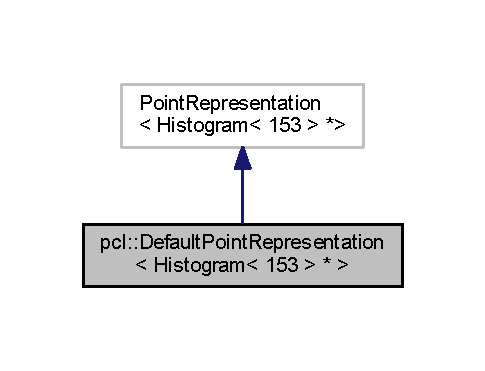
\includegraphics[width=233pt]{classpcl_1_1_default_point_representation_3_01_histogram_3_01153_01_4_01_5_01_4__inherit__graph}
\end{center}
\end{figure}


Collaboration diagram for pcl\+:\+:Default\+Point\+Representation$<$ Histogram$<$ 153 $>$ $\ast$ $>$\+:
\nopagebreak
\begin{figure}[H]
\begin{center}
\leavevmode
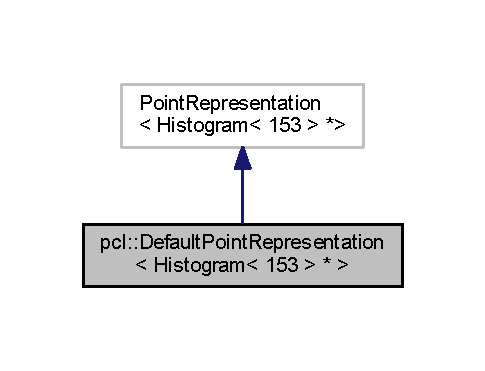
\includegraphics[width=233pt]{classpcl_1_1_default_point_representation_3_01_histogram_3_01153_01_4_01_5_01_4__coll__graph}
\end{center}
\end{figure}
\subsection*{Public Member Functions}
\begin{DoxyCompactItemize}
\item 
\hyperlink{classpcl_1_1_default_point_representation_3_01_histogram_3_01153_01_4_01_5_01_4_a7c00daa641cce7da6ab0ff49e248b351}{Default\+Point\+Representation} ()
\item 
virtual void \hyperlink{classpcl_1_1_default_point_representation_3_01_histogram_3_01153_01_4_01_5_01_4_af9596e041f0502152f0e2673f9f2358d}{copy\+To\+Float\+Array} (const Histogram$<$ 153 $>$ $\ast$p, float $\ast$out) const
\end{DoxyCompactItemize}


\subsection{Detailed Description}
\subsubsection*{template$<$$>$\newline
class pcl\+::\+Default\+Point\+Representation$<$ Histogram$<$ 153 $>$ $\ast$ $>$}



Definition at line 25 of file Default\+Point\+Representation.\+h.



\subsection{Constructor \& Destructor Documentation}
\mbox{\Hypertarget{classpcl_1_1_default_point_representation_3_01_histogram_3_01153_01_4_01_5_01_4_a7c00daa641cce7da6ab0ff49e248b351}\label{classpcl_1_1_default_point_representation_3_01_histogram_3_01153_01_4_01_5_01_4_a7c00daa641cce7da6ab0ff49e248b351}} 
\index{pcl\+::\+Default\+Point\+Representation$<$ Histogram$<$ 153 $>$ $\ast$ $>$@{pcl\+::\+Default\+Point\+Representation$<$ Histogram$<$ 153 $>$ $\ast$ $>$}!Default\+Point\+Representation@{Default\+Point\+Representation}}
\index{Default\+Point\+Representation@{Default\+Point\+Representation}!pcl\+::\+Default\+Point\+Representation$<$ Histogram$<$ 153 $>$ $\ast$ $>$@{pcl\+::\+Default\+Point\+Representation$<$ Histogram$<$ 153 $>$ $\ast$ $>$}}
\subsubsection{\texorpdfstring{Default\+Point\+Representation()}{DefaultPointRepresentation()}}
{\footnotesize\ttfamily pcl\+::\+Default\+Point\+Representation$<$ Histogram$<$ 153 $>$ $\ast$ $>$\+::Default\+Point\+Representation (\begin{DoxyParamCaption}{ }\end{DoxyParamCaption})\hspace{0.3cm}{\ttfamily [inline]}}



Definition at line 29 of file Default\+Point\+Representation.\+h.



\subsection{Member Function Documentation}
\mbox{\Hypertarget{classpcl_1_1_default_point_representation_3_01_histogram_3_01153_01_4_01_5_01_4_af9596e041f0502152f0e2673f9f2358d}\label{classpcl_1_1_default_point_representation_3_01_histogram_3_01153_01_4_01_5_01_4_af9596e041f0502152f0e2673f9f2358d}} 
\index{pcl\+::\+Default\+Point\+Representation$<$ Histogram$<$ 153 $>$ $\ast$ $>$@{pcl\+::\+Default\+Point\+Representation$<$ Histogram$<$ 153 $>$ $\ast$ $>$}!copy\+To\+Float\+Array@{copy\+To\+Float\+Array}}
\index{copy\+To\+Float\+Array@{copy\+To\+Float\+Array}!pcl\+::\+Default\+Point\+Representation$<$ Histogram$<$ 153 $>$ $\ast$ $>$@{pcl\+::\+Default\+Point\+Representation$<$ Histogram$<$ 153 $>$ $\ast$ $>$}}
\subsubsection{\texorpdfstring{copy\+To\+Float\+Array()}{copyToFloatArray()}}
{\footnotesize\ttfamily virtual void pcl\+::\+Default\+Point\+Representation$<$ Histogram$<$ 153 $>$ $\ast$ $>$\+::copy\+To\+Float\+Array (\begin{DoxyParamCaption}\item[{const Histogram$<$ 153 $>$ $\ast$}]{p,  }\item[{float $\ast$}]{out }\end{DoxyParamCaption}) const\hspace{0.3cm}{\ttfamily [inline]}, {\ttfamily [virtual]}}



Definition at line 35 of file Default\+Point\+Representation.\+h.



The documentation for this class was generated from the following file\+:\begin{DoxyCompactItemize}
\item 
H\+:/\+M\+E\+I/sistemas inteligentes/tp2/\+S\+I\+\_\+\+C\+O\+D\+E/include/\hyperlink{_default_point_representation_8h}{Default\+Point\+Representation.\+h}\end{DoxyCompactItemize}

\hypertarget{classpcl_1_1_default_point_representation_3_01_histogram_3_01153_01_4_01_4}{}\section{pcl\+:\+:Default\+Point\+Representation$<$ Histogram$<$ 153 $>$ $>$ Class Template Reference}
\label{classpcl_1_1_default_point_representation_3_01_histogram_3_01153_01_4_01_4}\index{pcl\+::\+Default\+Point\+Representation$<$ Histogram$<$ 153 $>$ $>$@{pcl\+::\+Default\+Point\+Representation$<$ Histogram$<$ 153 $>$ $>$}}


{\ttfamily \#include $<$Default\+Point\+Representation.\+h$>$}



Inheritance diagram for pcl\+:\+:Default\+Point\+Representation$<$ Histogram$<$ 153 $>$ $>$\+:
\nopagebreak
\begin{figure}[H]
\begin{center}
\leavevmode
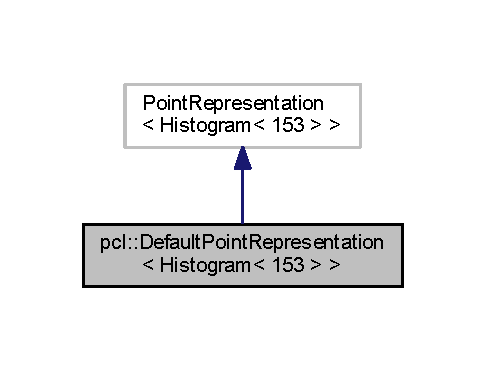
\includegraphics[width=233pt]{classpcl_1_1_default_point_representation_3_01_histogram_3_01153_01_4_01_4__inherit__graph}
\end{center}
\end{figure}


Collaboration diagram for pcl\+:\+:Default\+Point\+Representation$<$ Histogram$<$ 153 $>$ $>$\+:
\nopagebreak
\begin{figure}[H]
\begin{center}
\leavevmode
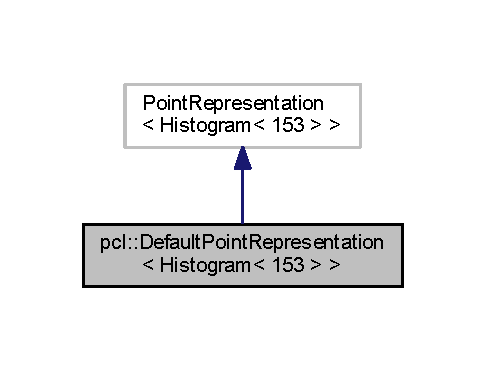
\includegraphics[width=233pt]{classpcl_1_1_default_point_representation_3_01_histogram_3_01153_01_4_01_4__coll__graph}
\end{center}
\end{figure}
\subsection*{Public Member Functions}
\begin{DoxyCompactItemize}
\item 
\hyperlink{classpcl_1_1_default_point_representation_3_01_histogram_3_01153_01_4_01_4_af423b3d8c452288ca14a44e97173c8bb}{Default\+Point\+Representation} ()
\item 
virtual void \hyperlink{classpcl_1_1_default_point_representation_3_01_histogram_3_01153_01_4_01_4_aa87167229f126da0b0ccff89887875ac}{copy\+To\+Float\+Array} (const Histogram$<$ 153 $>$ \&p, float $\ast$out) const
\end{DoxyCompactItemize}


\subsection{Detailed Description}
\subsubsection*{template$<$$>$\newline
class pcl\+::\+Default\+Point\+Representation$<$ Histogram$<$ 153 $>$ $>$}



Definition at line 5 of file Default\+Point\+Representation.\+h.



\subsection{Constructor \& Destructor Documentation}
\mbox{\Hypertarget{classpcl_1_1_default_point_representation_3_01_histogram_3_01153_01_4_01_4_af423b3d8c452288ca14a44e97173c8bb}\label{classpcl_1_1_default_point_representation_3_01_histogram_3_01153_01_4_01_4_af423b3d8c452288ca14a44e97173c8bb}} 
\index{pcl\+::\+Default\+Point\+Representation$<$ Histogram$<$ 153 $>$ $>$@{pcl\+::\+Default\+Point\+Representation$<$ Histogram$<$ 153 $>$ $>$}!Default\+Point\+Representation@{Default\+Point\+Representation}}
\index{Default\+Point\+Representation@{Default\+Point\+Representation}!pcl\+::\+Default\+Point\+Representation$<$ Histogram$<$ 153 $>$ $>$@{pcl\+::\+Default\+Point\+Representation$<$ Histogram$<$ 153 $>$ $>$}}
\subsubsection{\texorpdfstring{Default\+Point\+Representation()}{DefaultPointRepresentation()}}
{\footnotesize\ttfamily pcl\+::\+Default\+Point\+Representation$<$ Histogram$<$ 153 $>$ $>$\+::Default\+Point\+Representation (\begin{DoxyParamCaption}{ }\end{DoxyParamCaption})\hspace{0.3cm}{\ttfamily [inline]}}



Definition at line 9 of file Default\+Point\+Representation.\+h.



\subsection{Member Function Documentation}
\mbox{\Hypertarget{classpcl_1_1_default_point_representation_3_01_histogram_3_01153_01_4_01_4_aa87167229f126da0b0ccff89887875ac}\label{classpcl_1_1_default_point_representation_3_01_histogram_3_01153_01_4_01_4_aa87167229f126da0b0ccff89887875ac}} 
\index{pcl\+::\+Default\+Point\+Representation$<$ Histogram$<$ 153 $>$ $>$@{pcl\+::\+Default\+Point\+Representation$<$ Histogram$<$ 153 $>$ $>$}!copy\+To\+Float\+Array@{copy\+To\+Float\+Array}}
\index{copy\+To\+Float\+Array@{copy\+To\+Float\+Array}!pcl\+::\+Default\+Point\+Representation$<$ Histogram$<$ 153 $>$ $>$@{pcl\+::\+Default\+Point\+Representation$<$ Histogram$<$ 153 $>$ $>$}}
\subsubsection{\texorpdfstring{copy\+To\+Float\+Array()}{copyToFloatArray()}}
{\footnotesize\ttfamily virtual void pcl\+::\+Default\+Point\+Representation$<$ Histogram$<$ 153 $>$ $>$\+::copy\+To\+Float\+Array (\begin{DoxyParamCaption}\item[{const Histogram$<$ 153 $>$ \&}]{p,  }\item[{float $\ast$}]{out }\end{DoxyParamCaption}) const\hspace{0.3cm}{\ttfamily [inline]}, {\ttfamily [virtual]}}



Definition at line 15 of file Default\+Point\+Representation.\+h.



The documentation for this class was generated from the following file\+:\begin{DoxyCompactItemize}
\item 
H\+:/\+M\+E\+I/sistemas inteligentes/tp2/\+S\+I\+\_\+\+C\+O\+D\+E/include/\hyperlink{_default_point_representation_8h}{Default\+Point\+Representation.\+h}\end{DoxyCompactItemize}

\hypertarget{classpcl_1_1_default_point_representation_3_01_spin_image_01_4}{}\section{pcl\+:\+:Default\+Point\+Representation$<$ Spin\+Image $>$ Class Template Reference}
\label{classpcl_1_1_default_point_representation_3_01_spin_image_01_4}\index{pcl\+::\+Default\+Point\+Representation$<$ Spin\+Image $>$@{pcl\+::\+Default\+Point\+Representation$<$ Spin\+Image $>$}}


Inheritance diagram for pcl\+:\+:Default\+Point\+Representation$<$ Spin\+Image $>$\+:
\nopagebreak
\begin{figure}[H]
\begin{center}
\leavevmode
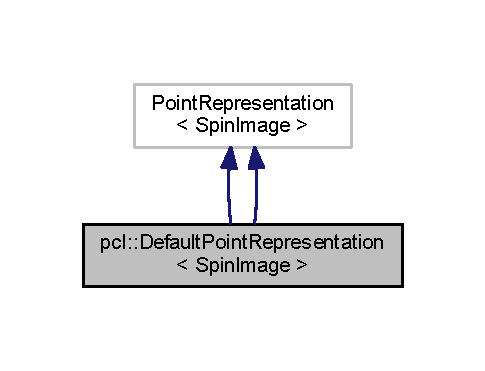
\includegraphics[width=233pt]{classpcl_1_1_default_point_representation_3_01_spin_image_01_4__inherit__graph}
\end{center}
\end{figure}


Collaboration diagram for pcl\+:\+:Default\+Point\+Representation$<$ Spin\+Image $>$\+:
\nopagebreak
\begin{figure}[H]
\begin{center}
\leavevmode
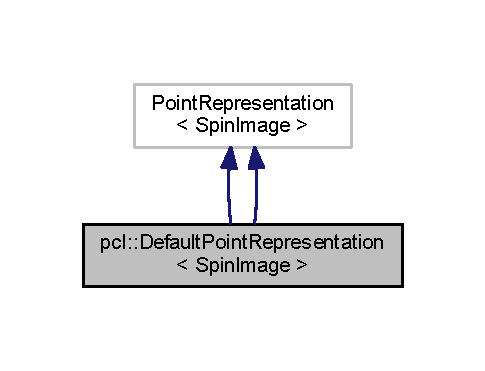
\includegraphics[width=233pt]{classpcl_1_1_default_point_representation_3_01_spin_image_01_4__coll__graph}
\end{center}
\end{figure}
\subsection*{Public Member Functions}
\begin{DoxyCompactItemize}
\item 
\hyperlink{classpcl_1_1_default_point_representation_3_01_spin_image_01_4_afa348f01d1192b29c50649a4a3cfadb9}{Default\+Point\+Representation} ()
\item 
virtual void \hyperlink{classpcl_1_1_default_point_representation_3_01_spin_image_01_4_af51ac110bddbb250714b11d268c6ea73}{copy\+To\+Float\+Array} (const \hyperlink{include_8h_ab79ade12a22a8e5e2864650f820e9c6f}{Spin\+Image} \&p, float $\ast$out) const
\item 
\hyperlink{classpcl_1_1_default_point_representation_3_01_spin_image_01_4_afa348f01d1192b29c50649a4a3cfadb9}{Default\+Point\+Representation} ()
\item 
virtual void \hyperlink{classpcl_1_1_default_point_representation_3_01_spin_image_01_4_af51ac110bddbb250714b11d268c6ea73}{copy\+To\+Float\+Array} (const \hyperlink{include_8h_ab79ade12a22a8e5e2864650f820e9c6f}{Spin\+Image} \&p, float $\ast$out) const
\end{DoxyCompactItemize}


\subsection{Detailed Description}
\subsubsection*{template$<$$>$\newline
class pcl\+::\+Default\+Point\+Representation$<$ Spin\+Image $>$}



Definition at line 17 of file Memory.\+cpp.



\subsection{Constructor \& Destructor Documentation}
\mbox{\Hypertarget{classpcl_1_1_default_point_representation_3_01_spin_image_01_4_afa348f01d1192b29c50649a4a3cfadb9}\label{classpcl_1_1_default_point_representation_3_01_spin_image_01_4_afa348f01d1192b29c50649a4a3cfadb9}} 
\index{pcl\+::\+Default\+Point\+Representation$<$ Spin\+Image $>$@{pcl\+::\+Default\+Point\+Representation$<$ Spin\+Image $>$}!Default\+Point\+Representation@{Default\+Point\+Representation}}
\index{Default\+Point\+Representation@{Default\+Point\+Representation}!pcl\+::\+Default\+Point\+Representation$<$ Spin\+Image $>$@{pcl\+::\+Default\+Point\+Representation$<$ Spin\+Image $>$}}
\subsubsection{\texorpdfstring{Default\+Point\+Representation()}{DefaultPointRepresentation()}\hspace{0.1cm}{\footnotesize\ttfamily [1/2]}}
{\footnotesize\ttfamily pcl\+::\+Default\+Point\+Representation$<$ \hyperlink{include_8h_ab79ade12a22a8e5e2864650f820e9c6f}{Spin\+Image} $>$\+::Default\+Point\+Representation (\begin{DoxyParamCaption}{ }\end{DoxyParamCaption})\hspace{0.3cm}{\ttfamily [inline]}}



Definition at line 20 of file Memory.\+cpp.

\mbox{\Hypertarget{classpcl_1_1_default_point_representation_3_01_spin_image_01_4_afa348f01d1192b29c50649a4a3cfadb9}\label{classpcl_1_1_default_point_representation_3_01_spin_image_01_4_afa348f01d1192b29c50649a4a3cfadb9}} 
\index{pcl\+::\+Default\+Point\+Representation$<$ Spin\+Image $>$@{pcl\+::\+Default\+Point\+Representation$<$ Spin\+Image $>$}!Default\+Point\+Representation@{Default\+Point\+Representation}}
\index{Default\+Point\+Representation@{Default\+Point\+Representation}!pcl\+::\+Default\+Point\+Representation$<$ Spin\+Image $>$@{pcl\+::\+Default\+Point\+Representation$<$ Spin\+Image $>$}}
\subsubsection{\texorpdfstring{Default\+Point\+Representation()}{DefaultPointRepresentation()}\hspace{0.1cm}{\footnotesize\ttfamily [2/2]}}
{\footnotesize\ttfamily pcl\+::\+Default\+Point\+Representation$<$ \hyperlink{include_8h_ab79ade12a22a8e5e2864650f820e9c6f}{Spin\+Image} $>$\+::Default\+Point\+Representation (\begin{DoxyParamCaption}{ }\end{DoxyParamCaption})\hspace{0.3cm}{\ttfamily [inline]}}



Definition at line 10 of file Searcher.\+cpp.



\subsection{Member Function Documentation}
\mbox{\Hypertarget{classpcl_1_1_default_point_representation_3_01_spin_image_01_4_af51ac110bddbb250714b11d268c6ea73}\label{classpcl_1_1_default_point_representation_3_01_spin_image_01_4_af51ac110bddbb250714b11d268c6ea73}} 
\index{pcl\+::\+Default\+Point\+Representation$<$ Spin\+Image $>$@{pcl\+::\+Default\+Point\+Representation$<$ Spin\+Image $>$}!copy\+To\+Float\+Array@{copy\+To\+Float\+Array}}
\index{copy\+To\+Float\+Array@{copy\+To\+Float\+Array}!pcl\+::\+Default\+Point\+Representation$<$ Spin\+Image $>$@{pcl\+::\+Default\+Point\+Representation$<$ Spin\+Image $>$}}
\subsubsection{\texorpdfstring{copy\+To\+Float\+Array()}{copyToFloatArray()}\hspace{0.1cm}{\footnotesize\ttfamily [1/2]}}
{\footnotesize\ttfamily virtual void pcl\+::\+Default\+Point\+Representation$<$ \hyperlink{include_8h_ab79ade12a22a8e5e2864650f820e9c6f}{Spin\+Image} $>$\+::copy\+To\+Float\+Array (\begin{DoxyParamCaption}\item[{const \hyperlink{include_8h_ab79ade12a22a8e5e2864650f820e9c6f}{Spin\+Image} \&}]{p,  }\item[{float $\ast$}]{out }\end{DoxyParamCaption}) const\hspace{0.3cm}{\ttfamily [inline]}, {\ttfamily [virtual]}}



Definition at line 15 of file Searcher.\+cpp.

\mbox{\Hypertarget{classpcl_1_1_default_point_representation_3_01_spin_image_01_4_af51ac110bddbb250714b11d268c6ea73}\label{classpcl_1_1_default_point_representation_3_01_spin_image_01_4_af51ac110bddbb250714b11d268c6ea73}} 
\index{pcl\+::\+Default\+Point\+Representation$<$ Spin\+Image $>$@{pcl\+::\+Default\+Point\+Representation$<$ Spin\+Image $>$}!copy\+To\+Float\+Array@{copy\+To\+Float\+Array}}
\index{copy\+To\+Float\+Array@{copy\+To\+Float\+Array}!pcl\+::\+Default\+Point\+Representation$<$ Spin\+Image $>$@{pcl\+::\+Default\+Point\+Representation$<$ Spin\+Image $>$}}
\subsubsection{\texorpdfstring{copy\+To\+Float\+Array()}{copyToFloatArray()}\hspace{0.1cm}{\footnotesize\ttfamily [2/2]}}
{\footnotesize\ttfamily virtual void pcl\+::\+Default\+Point\+Representation$<$ \hyperlink{include_8h_ab79ade12a22a8e5e2864650f820e9c6f}{Spin\+Image} $>$\+::copy\+To\+Float\+Array (\begin{DoxyParamCaption}\item[{const \hyperlink{include_8h_ab79ade12a22a8e5e2864650f820e9c6f}{Spin\+Image} \&}]{p,  }\item[{float $\ast$}]{out }\end{DoxyParamCaption}) const\hspace{0.3cm}{\ttfamily [inline]}, {\ttfamily [virtual]}}



Definition at line 25 of file Memory.\+cpp.



The documentation for this class was generated from the following files\+:\begin{DoxyCompactItemize}
\item 
H\+:/\+M\+E\+I/sistemas inteligentes/tp2/\+S\+I\+\_\+\+C\+O\+D\+E/src/\hyperlink{_memory_8cpp}{Memory.\+cpp}\item 
H\+:/\+M\+E\+I/sistemas inteligentes/tp2/\+S\+I\+\_\+\+C\+O\+D\+E/src/\hyperlink{_searcher_8cpp}{Searcher.\+cpp}\end{DoxyCompactItemize}

\hypertarget{structdescending}{}\section{descending Struct Reference}
\label{structdescending}\index{descending@{descending}}


Operator used with std\+:sort to sort a vector$<$pair$<$int, float$>$ $>$ by the value of the pair (the second argument of the pair, the float) in descending order.  




{\ttfamily \#include $<$Memory.\+h$>$}

\subsection*{Public Member Functions}
\begin{DoxyCompactItemize}
\item 
bool \hyperlink{structdescending_a40cf683917ac8db4a163427d9585e5af}{operator()} (const std\+::pair$<$ int, \hyperlink{class_wss_bag}{Wss\+Bag} $>$ \&left, const std\+::pair$<$ int, \hyperlink{class_wss_bag}{Wss\+Bag} $>$ \&right)
\end{DoxyCompactItemize}


\subsection{Detailed Description}
Operator used with std\+:sort to sort a vector$<$pair$<$int, float$>$ $>$ by the value of the pair (the second argument of the pair, the float) in descending order. 

Definition at line 820 of file Memory.\+h.



\subsection{Member Function Documentation}
\mbox{\Hypertarget{structdescending_a40cf683917ac8db4a163427d9585e5af}\label{structdescending_a40cf683917ac8db4a163427d9585e5af}} 
\index{descending@{descending}!operator()@{operator()}}
\index{operator()@{operator()}!descending@{descending}}
\subsubsection{\texorpdfstring{operator()()}{operator()()}}
{\footnotesize\ttfamily bool descending\+::operator() (\begin{DoxyParamCaption}\item[{const std\+::pair$<$ int, \hyperlink{class_wss_bag}{Wss\+Bag} $>$ \&}]{left,  }\item[{const std\+::pair$<$ int, \hyperlink{class_wss_bag}{Wss\+Bag} $>$ \&}]{right }\end{DoxyParamCaption})\hspace{0.3cm}{\ttfamily [inline]}}



Definition at line 822 of file Memory.\+h.



The documentation for this struct was generated from the following file\+:\begin{DoxyCompactItemize}
\item 
H\+:/\+M\+E\+I/sistemas inteligentes/tp2/\+S\+I\+\_\+\+C\+O\+D\+E/include/\hyperlink{_memory_8h}{Memory.\+h}\end{DoxyCompactItemize}

\hypertarget{class_feature_extractor}{}\section{Feature\+Extractor Class Reference}
\label{class_feature_extractor}\index{Feature\+Extractor@{Feature\+Extractor}}


Functions to extract keypoints from a point cloud and compute spin images.  




{\ttfamily \#include $<$Feature\+Extractor.\+h$>$}

\subsection*{Public Member Functions}
\begin{DoxyCompactItemize}
\item 
\hyperlink{class_feature_extractor_a58c705d663551bfa7baea3d75614311f}{Feature\+Extractor} ()
\item 
\hyperlink{class_feature_extractor_ad87b36879a01dcfe45f57318d2850c54}{$\sim$\+Feature\+Extractor} ()
\item 
void \hyperlink{class_feature_extractor_aa9dc5acc77de1af1f320c131a81a0928}{Get\+Keypoints\+Using\+A\+Voxel\+Filter} (const Point\+Cloud$<$ \hyperlink{include_8h_a6ca7710b84e9152e036423253ffc1ae7}{PointT} $>$\+::Ptr \&pc, float voxel\+Size, Point\+Cloud$<$ \hyperlink{include_8h_a6ca7710b84e9152e036423253ffc1ae7}{PointT} $>$\+::Ptr \&keypoints) const
\item 
void \hyperlink{class_feature_extractor_ad977ae7b163c09dd44b488c80a0a201c}{Compute\+Spin\+Images\+At\+Keypoints} (const Point\+Cloud$<$ \hyperlink{include_8h_a6ca7710b84e9152e036423253ffc1ae7}{PointT} $>$\+::Ptr \&search\+\_\+surface, const Point\+Cloud$<$ \hyperlink{include_8h_a6ca7710b84e9152e036423253ffc1ae7}{PointT} $>$\+::Ptr \&keypoints, float radius\+\_\+search, int \hyperlink{pcd__read_8cpp_a0e2e740afd510cfe652a1836ffbad209}{window\+\_\+width}, float \hyperlink{pcd__read_8cpp_abed5c1c3716fc66df9f1a01a430aa8cc}{support\+\_\+lenght}, float \hyperlink{pcd__read_8cpp_a13fd0ebf6c809f68d2b0e9bfc16bf68d}{support\+\_\+angle}, float \hyperlink{pcd__read_8cpp_abbd3dac675fcfc5a5b1d4650518f3771}{min\+\_\+pts\+\_\+neighbours}, Point\+Cloud$<$ \hyperlink{include_8h_ab79ade12a22a8e5e2864650f820e9c6f}{Spin\+Image} $>$\+::Ptr \&spin\+\_\+images) const
\item 
void \hyperlink{class_feature_extractor_a7612f1c3b17030d24a89b44973fd109e}{Compute\+Surface\+Normals} (const Point\+Cloud$<$ \hyperlink{include_8h_a6ca7710b84e9152e036423253ffc1ae7}{PointT} $>$\+::Ptr \&pc, float normal\+\_\+radius, Point\+Cloud$<$ Normal $>$\+::Ptr \&pc\+\_\+normals\+\_\+out) const
\end{DoxyCompactItemize}


\subsection{Detailed Description}
Functions to extract keypoints from a point cloud and compute spin images. 

In this version the keypoints are extracted using a voxel grid filter. 

Definition at line 11 of file Feature\+Extractor.\+h.



\subsection{Constructor \& Destructor Documentation}
\mbox{\Hypertarget{class_feature_extractor_a58c705d663551bfa7baea3d75614311f}\label{class_feature_extractor_a58c705d663551bfa7baea3d75614311f}} 
\index{Feature\+Extractor@{Feature\+Extractor}!Feature\+Extractor@{Feature\+Extractor}}
\index{Feature\+Extractor@{Feature\+Extractor}!Feature\+Extractor@{Feature\+Extractor}}
\subsubsection{\texorpdfstring{Feature\+Extractor()}{FeatureExtractor()}}
{\footnotesize\ttfamily Feature\+Extractor\+::\+Feature\+Extractor (\begin{DoxyParamCaption}{ }\end{DoxyParamCaption})}



Definition at line 4 of file Feature\+Extractor.\+cpp.

\mbox{\Hypertarget{class_feature_extractor_ad87b36879a01dcfe45f57318d2850c54}\label{class_feature_extractor_ad87b36879a01dcfe45f57318d2850c54}} 
\index{Feature\+Extractor@{Feature\+Extractor}!````~Feature\+Extractor@{$\sim$\+Feature\+Extractor}}
\index{````~Feature\+Extractor@{$\sim$\+Feature\+Extractor}!Feature\+Extractor@{Feature\+Extractor}}
\subsubsection{\texorpdfstring{$\sim$\+Feature\+Extractor()}{~FeatureExtractor()}}
{\footnotesize\ttfamily Feature\+Extractor\+::$\sim$\+Feature\+Extractor (\begin{DoxyParamCaption}{ }\end{DoxyParamCaption})}



Definition at line 7 of file Feature\+Extractor.\+cpp.



\subsection{Member Function Documentation}
\mbox{\Hypertarget{class_feature_extractor_ad977ae7b163c09dd44b488c80a0a201c}\label{class_feature_extractor_ad977ae7b163c09dd44b488c80a0a201c}} 
\index{Feature\+Extractor@{Feature\+Extractor}!Compute\+Spin\+Images\+At\+Keypoints@{Compute\+Spin\+Images\+At\+Keypoints}}
\index{Compute\+Spin\+Images\+At\+Keypoints@{Compute\+Spin\+Images\+At\+Keypoints}!Feature\+Extractor@{Feature\+Extractor}}
\subsubsection{\texorpdfstring{Compute\+Spin\+Images\+At\+Keypoints()}{ComputeSpinImagesAtKeypoints()}}
{\footnotesize\ttfamily void Feature\+Extractor\+::\+Compute\+Spin\+Images\+At\+Keypoints (\begin{DoxyParamCaption}\item[{const Point\+Cloud$<$ \hyperlink{include_8h_a6ca7710b84e9152e036423253ffc1ae7}{PointT} $>$\+::Ptr \&}]{search\+\_\+surface,  }\item[{const Point\+Cloud$<$ \hyperlink{include_8h_a6ca7710b84e9152e036423253ffc1ae7}{PointT} $>$\+::Ptr \&}]{keypoints,  }\item[{float}]{radius\+\_\+search,  }\item[{int}]{window\+\_\+width,  }\item[{float}]{support\+\_\+lenght,  }\item[{float}]{support\+\_\+angle,  }\item[{float}]{min\+\_\+pts\+\_\+neighbours,  }\item[{Point\+Cloud$<$ \hyperlink{include_8h_ab79ade12a22a8e5e2864650f820e9c6f}{Spin\+Image} $>$\+::Ptr \&}]{spin\+\_\+images }\end{DoxyParamCaption}) const}

Computes spin images for a set of given points.


\begin{DoxyParams}[1]{Parameters}
\mbox{\tt in}  & {\em search\+\_\+surface} & the search surface \\
\hline
\mbox{\tt in}  & {\em keypoints} & the keypoints, points, to get the spin images for \\
\hline
\mbox{\tt in}  & {\em radius\+\_\+search} & paremeters for spin image generation \\
\hline
\mbox{\tt in}  & {\em window\+\_\+width} & \\
\hline
\mbox{\tt in}  & {\em support\+\_\+lenght} & \\
\hline
\mbox{\tt in}  & {\em support\+\_\+angle} & \\
\hline
\mbox{\tt in}  & {\em min\+\_\+pts\+\_\+neighbours} & \\
\hline
\mbox{\tt out}  & {\em spin\+\_\+images} & the computed spin images for each point \\
\hline
\end{DoxyParams}


Definition at line 20 of file Feature\+Extractor.\+cpp.

\mbox{\Hypertarget{class_feature_extractor_a7612f1c3b17030d24a89b44973fd109e}\label{class_feature_extractor_a7612f1c3b17030d24a89b44973fd109e}} 
\index{Feature\+Extractor@{Feature\+Extractor}!Compute\+Surface\+Normals@{Compute\+Surface\+Normals}}
\index{Compute\+Surface\+Normals@{Compute\+Surface\+Normals}!Feature\+Extractor@{Feature\+Extractor}}
\subsubsection{\texorpdfstring{Compute\+Surface\+Normals()}{ComputeSurfaceNormals()}}
{\footnotesize\ttfamily void Feature\+Extractor\+::\+Compute\+Surface\+Normals (\begin{DoxyParamCaption}\item[{const Point\+Cloud$<$ \hyperlink{include_8h_a6ca7710b84e9152e036423253ffc1ae7}{PointT} $>$\+::Ptr \&}]{pc,  }\item[{float}]{normal\+\_\+radius,  }\item[{Point\+Cloud$<$ Normal $>$\+::Ptr \&}]{pc\+\_\+normals\+\_\+out }\end{DoxyParamCaption}) const}

Computes the surface normals.


\begin{DoxyParams}[1]{Parameters}
\mbox{\tt in}  & {\em pc} & the point cloud \\
\hline
\mbox{\tt in}  & {\em normal\+\_\+radius} & paremeter for normals computation \\
\hline
\mbox{\tt out}  & {\em pc\+\_\+normals\+\_\+out} & the point cloud computed normals \\
\hline
\end{DoxyParams}


Definition at line 50 of file Feature\+Extractor.\+cpp.

\mbox{\Hypertarget{class_feature_extractor_aa9dc5acc77de1af1f320c131a81a0928}\label{class_feature_extractor_aa9dc5acc77de1af1f320c131a81a0928}} 
\index{Feature\+Extractor@{Feature\+Extractor}!Get\+Keypoints\+Using\+A\+Voxel\+Filter@{Get\+Keypoints\+Using\+A\+Voxel\+Filter}}
\index{Get\+Keypoints\+Using\+A\+Voxel\+Filter@{Get\+Keypoints\+Using\+A\+Voxel\+Filter}!Feature\+Extractor@{Feature\+Extractor}}
\subsubsection{\texorpdfstring{Get\+Keypoints\+Using\+A\+Voxel\+Filter()}{GetKeypointsUsingAVoxelFilter()}}
{\footnotesize\ttfamily void Feature\+Extractor\+::\+Get\+Keypoints\+Using\+A\+Voxel\+Filter (\begin{DoxyParamCaption}\item[{const Point\+Cloud$<$ \hyperlink{include_8h_a6ca7710b84e9152e036423253ffc1ae7}{PointT} $>$\+::Ptr \&}]{pc,  }\item[{float}]{voxel\+Size,  }\item[{Point\+Cloud$<$ \hyperlink{include_8h_a6ca7710b84e9152e036423253ffc1ae7}{PointT} $>$\+::Ptr \&}]{keypoints }\end{DoxyParamCaption}) const}

Find keypoints using a Voxel Grid Filter.


\begin{DoxyParams}[1]{Parameters}
\mbox{\tt in}  & {\em pc} & the point cloud to get keypoints from \\
\hline
\mbox{\tt in}  & {\em voxel\+Size} & the voxel grid filter size \\
\hline
\mbox{\tt out}  & {\em keypoints} & the keypoints found using the Voxel Grid Filter \\
\hline
\end{DoxyParams}


Definition at line 10 of file Feature\+Extractor.\+cpp.



The documentation for this class was generated from the following files\+:\begin{DoxyCompactItemize}
\item 
H\+:/\+M\+E\+I/sistemas inteligentes/tp2/\+S\+I\+\_\+\+C\+O\+D\+E/include/\hyperlink{_feature_extractor_8h}{Feature\+Extractor.\+h}\item 
H\+:/\+M\+E\+I/sistemas inteligentes/tp2/\+S\+I\+\_\+\+C\+O\+D\+E/src/\hyperlink{_feature_extractor_8cpp}{Feature\+Extractor.\+cpp}\end{DoxyCompactItemize}

\hypertarget{class_feature_metadata}{}\section{Feature\+Metadata Class Reference}
\label{class_feature_metadata}\index{Feature\+Metadata@{Feature\+Metadata}}


Holds metadata about a feature as well as the feature itself.  




{\ttfamily \#include $<$Feature\+Metadata.\+h$>$}

\subsection*{Public Member Functions}
\begin{DoxyCompactItemize}
\item 
\hyperlink{class_feature_metadata_ab117cd690bb70fe8795422f976a251d7}{Feature\+Metadata} ()
\item 
\hyperlink{class_feature_metadata_ac94095ccb8ba325b552dd192c86bce09}{Feature\+Metadata} (const \hyperlink{class_feature_metadata}{Feature\+Metadata} \&obj)
\item 
\hyperlink{class_feature_metadata_a1374c7d4f2e24bf0cf343949eeb93422}{Feature\+Metadata} (pcl\+::\+Histogram$<$ 153 $>$ \&\hyperlink{class_feature_metadata_a0b288799d230ccf13d34efd60165ebb6}{feature}, float \hyperlink{class_feature_metadata_a5b7a2efcdc98b2fc62fd7e47eceed296}{l\+Weight}=1, float \hyperlink{class_feature_metadata_acb096e77efd9a31c51b99682160324ce}{g\+Weight}=1, int \hyperlink{class_feature_metadata_a722c6a86c099fc76fe4d25aedaf98c1c}{count}=1, int \hyperlink{class_feature_metadata_a7f5a6347721de970e0dd5abf4b0a8455}{cluster}=-\/1, float \hyperlink{class_feature_metadata_ab8a28f696d38b7bdd3aeef92a3453bcf}{d\+Cluster\+Centroid}=0, int \hyperlink{class_feature_metadata_a30e96aabc8090f41b8136cbb274da383}{category}=-\/1)
\item 
float \hyperlink{class_feature_metadata_a03bdbfab84fa2b98930093657d40735c}{get\+Local\+Weight} () const
\item 
void \hyperlink{class_feature_metadata_a48c33c739f9ee12a04c3cf01a09d4f47}{set\+Local\+Weight} (float val)
\item 
float \hyperlink{class_feature_metadata_a0ba779c2a9d106b987edc306b14f3191}{get\+Global\+Weight} () const
\item 
void \hyperlink{class_feature_metadata_a135f89c383379bee9943acec65d3bdeb}{set\+Global\+Weight} (float val)
\item 
int \hyperlink{class_feature_metadata_a4691adf4f46586826fd8c0667119fc52}{get\+Cluster} () const
\item 
bool \hyperlink{class_feature_metadata_a896922c34a6bf90f4c22b8e9546108dc}{assign\+To\+Cluster} (int n\+Cluster)
\item 
void \hyperlink{class_feature_metadata_a203acc4e77eaf40cb42ac446c92af241}{un\+Assign\+From\+Cluster} ()
\item 
const float \hyperlink{class_feature_metadata_a4736658ecb89297dd9bad9c701f59e8f}{get\+Distance\+To\+Centroid} () const
\item 
const int \hyperlink{class_feature_metadata_a52510d086e0b5fdc1b34b718c3bebd14}{get\+Count} () const
\item 
pcl\+::\+Histogram$<$ 153 $>$ \& \hyperlink{class_feature_metadata_a92f0b1da1d3892508fa358a58946060a}{get\+Feature} ()
\item 
void \hyperlink{class_feature_metadata_abd9ec7695ed8e497aa1101695d3b5143}{set\+Distance\+To\+Centroid} (float val)
\item 
int \hyperlink{class_feature_metadata_a8121654a5fc7422adb41cd04ddb0bc72}{get\+Category} () const
\item 
void \hyperlink{class_feature_metadata_acc32427e65eab74731498c4a3f0eca34}{assign\+To\+Category} (int n\+Category)
\item 
void \hyperlink{class_feature_metadata_a64772c40574899bb2b3985b1bea2a819}{un\+Assign\+From\+Category} ()
\item 
void \hyperlink{class_feature_metadata_acbb60bf43880c89dacd3a81b4e2d0c43}{set\+Feature} (pcl\+::\+Histogram$<$ 153 $>$ \&feat)
\item 
void \hyperlink{class_feature_metadata_a2c493838e535578c670052b08b61d069}{add\+Count} ()
\end{DoxyCompactItemize}
\subsection*{Protected Attributes}
\begin{DoxyCompactItemize}
\item 
pcl\+::\+Histogram$<$ 153 $>$ \hyperlink{class_feature_metadata_a0b288799d230ccf13d34efd60165ebb6}{feature}
\item 
float \hyperlink{class_feature_metadata_a5b7a2efcdc98b2fc62fd7e47eceed296}{l\+Weight}
\item 
float \hyperlink{class_feature_metadata_acb096e77efd9a31c51b99682160324ce}{g\+Weight}
\item 
int \hyperlink{class_feature_metadata_a722c6a86c099fc76fe4d25aedaf98c1c}{count}
\item 
int \hyperlink{class_feature_metadata_a7f5a6347721de970e0dd5abf4b0a8455}{cluster}
\item 
float \hyperlink{class_feature_metadata_ab8a28f696d38b7bdd3aeef92a3453bcf}{d\+Cluster\+Centroid}
\item 
int \hyperlink{class_feature_metadata_a30e96aabc8090f41b8136cbb274da383}{category}
\end{DoxyCompactItemize}


\subsection{Detailed Description}
Holds metadata about a feature as well as the feature itself. 

Definition at line 14 of file Feature\+Metadata.\+h.



\subsection{Constructor \& Destructor Documentation}
\mbox{\Hypertarget{class_feature_metadata_ab117cd690bb70fe8795422f976a251d7}\label{class_feature_metadata_ab117cd690bb70fe8795422f976a251d7}} 
\index{Feature\+Metadata@{Feature\+Metadata}!Feature\+Metadata@{Feature\+Metadata}}
\index{Feature\+Metadata@{Feature\+Metadata}!Feature\+Metadata@{Feature\+Metadata}}
\subsubsection{\texorpdfstring{Feature\+Metadata()}{FeatureMetadata()}\hspace{0.1cm}{\footnotesize\ttfamily [1/3]}}
{\footnotesize\ttfamily Feature\+Metadata\+::\+Feature\+Metadata (\begin{DoxyParamCaption}{ }\end{DoxyParamCaption})\hspace{0.3cm}{\ttfamily [inline]}}

The empty constructor is required when used as the value in a map. But calling it is considered an error and is treated with an exception! 

Definition at line 20 of file Feature\+Metadata.\+h.

\mbox{\Hypertarget{class_feature_metadata_ac94095ccb8ba325b552dd192c86bce09}\label{class_feature_metadata_ac94095ccb8ba325b552dd192c86bce09}} 
\index{Feature\+Metadata@{Feature\+Metadata}!Feature\+Metadata@{Feature\+Metadata}}
\index{Feature\+Metadata@{Feature\+Metadata}!Feature\+Metadata@{Feature\+Metadata}}
\subsubsection{\texorpdfstring{Feature\+Metadata()}{FeatureMetadata()}\hspace{0.1cm}{\footnotesize\ttfamily [2/3]}}
{\footnotesize\ttfamily Feature\+Metadata\+::\+Feature\+Metadata (\begin{DoxyParamCaption}\item[{const \hyperlink{class_feature_metadata}{Feature\+Metadata} \&}]{obj }\end{DoxyParamCaption})\hspace{0.3cm}{\ttfamily [inline]}}

Copy constructor. T\+O\+DO; is this realy needed? 

Definition at line 29 of file Feature\+Metadata.\+h.

\mbox{\Hypertarget{class_feature_metadata_a1374c7d4f2e24bf0cf343949eeb93422}\label{class_feature_metadata_a1374c7d4f2e24bf0cf343949eeb93422}} 
\index{Feature\+Metadata@{Feature\+Metadata}!Feature\+Metadata@{Feature\+Metadata}}
\index{Feature\+Metadata@{Feature\+Metadata}!Feature\+Metadata@{Feature\+Metadata}}
\subsubsection{\texorpdfstring{Feature\+Metadata()}{FeatureMetadata()}\hspace{0.1cm}{\footnotesize\ttfamily [3/3]}}
{\footnotesize\ttfamily Feature\+Metadata\+::\+Feature\+Metadata (\begin{DoxyParamCaption}\item[{pcl\+::\+Histogram$<$ 153 $>$ \&}]{feature,  }\item[{float}]{l\+Weight = {\ttfamily 1},  }\item[{float}]{g\+Weight = {\ttfamily 1},  }\item[{int}]{count = {\ttfamily 1},  }\item[{int}]{cluster = {\ttfamily -\/1},  }\item[{float}]{d\+Cluster\+Centroid = {\ttfamily 0},  }\item[{int}]{category = {\ttfamily -\/1} }\end{DoxyParamCaption})}

Creates a new \char`\"{}feature\char`\"{}. Don\textquotesingle{}t use\+: count and d\+Cluster\+Centroid!


\begin{DoxyParams}[1]{Parameters}
\mbox{\tt in}  & {\em feature} & the feature \\
\hline
\mbox{\tt in}  & {\em l\+Weight} & the local weight of the feature (associated to the category the feature was assigned) \\
\hline
\mbox{\tt in}  & {\em g\+Weight} & the global weight of the feature (associated to the cluster the feature was assigned) \\
\hline
\mbox{\tt in}  & {\em count} & the number of similar features the feature represents \\
\hline
\mbox{\tt in}  & {\em cluster} & the cluster identifier (map key) to the cluster the feature was assigned to \\
\hline
\mbox{\tt in}  & {\em d\+Cluster\+Centroid} & the distace of the feature to the its cluster centroid \\
\hline
\mbox{\tt in}  & {\em category} & the category identifier (map key) to the category the feature was assigned to \\
\hline
\end{DoxyParams}


\subsection{Member Function Documentation}
\mbox{\Hypertarget{class_feature_metadata_a2c493838e535578c670052b08b61d069}\label{class_feature_metadata_a2c493838e535578c670052b08b61d069}} 
\index{Feature\+Metadata@{Feature\+Metadata}!add\+Count@{add\+Count}}
\index{add\+Count@{add\+Count}!Feature\+Metadata@{Feature\+Metadata}}
\subsubsection{\texorpdfstring{add\+Count()}{addCount()}}
{\footnotesize\ttfamily void Feature\+Metadata\+::add\+Count (\begin{DoxyParamCaption}{ }\end{DoxyParamCaption})\hspace{0.3cm}{\ttfamily [inline]}}

Don\textquotesingle{}t use this function! 

Definition at line 194 of file Feature\+Metadata.\+h.

\mbox{\Hypertarget{class_feature_metadata_acc32427e65eab74731498c4a3f0eca34}\label{class_feature_metadata_acc32427e65eab74731498c4a3f0eca34}} 
\index{Feature\+Metadata@{Feature\+Metadata}!assign\+To\+Category@{assign\+To\+Category}}
\index{assign\+To\+Category@{assign\+To\+Category}!Feature\+Metadata@{Feature\+Metadata}}
\subsubsection{\texorpdfstring{assign\+To\+Category()}{assignToCategory()}}
{\footnotesize\ttfamily void Feature\+Metadata\+::assign\+To\+Category (\begin{DoxyParamCaption}\item[{int}]{n\+Category }\end{DoxyParamCaption})\hspace{0.3cm}{\ttfamily [inline]}}



Definition at line 175 of file Feature\+Metadata.\+h.

\mbox{\Hypertarget{class_feature_metadata_a896922c34a6bf90f4c22b8e9546108dc}\label{class_feature_metadata_a896922c34a6bf90f4c22b8e9546108dc}} 
\index{Feature\+Metadata@{Feature\+Metadata}!assign\+To\+Cluster@{assign\+To\+Cluster}}
\index{assign\+To\+Cluster@{assign\+To\+Cluster}!Feature\+Metadata@{Feature\+Metadata}}
\subsubsection{\texorpdfstring{assign\+To\+Cluster()}{assignToCluster()}}
{\footnotesize\ttfamily bool Feature\+Metadata\+::assign\+To\+Cluster (\begin{DoxyParamCaption}\item[{int}]{n\+Cluster }\end{DoxyParamCaption})\hspace{0.3cm}{\ttfamily [inline]}}



Definition at line 129 of file Feature\+Metadata.\+h.

\mbox{\Hypertarget{class_feature_metadata_a8121654a5fc7422adb41cd04ddb0bc72}\label{class_feature_metadata_a8121654a5fc7422adb41cd04ddb0bc72}} 
\index{Feature\+Metadata@{Feature\+Metadata}!get\+Category@{get\+Category}}
\index{get\+Category@{get\+Category}!Feature\+Metadata@{Feature\+Metadata}}
\subsubsection{\texorpdfstring{get\+Category()}{getCategory()}}
{\footnotesize\ttfamily int Feature\+Metadata\+::get\+Category (\begin{DoxyParamCaption}{ }\end{DoxyParamCaption}) const\hspace{0.3cm}{\ttfamily [inline]}}



Definition at line 171 of file Feature\+Metadata.\+h.

\mbox{\Hypertarget{class_feature_metadata_a4691adf4f46586826fd8c0667119fc52}\label{class_feature_metadata_a4691adf4f46586826fd8c0667119fc52}} 
\index{Feature\+Metadata@{Feature\+Metadata}!get\+Cluster@{get\+Cluster}}
\index{get\+Cluster@{get\+Cluster}!Feature\+Metadata@{Feature\+Metadata}}
\subsubsection{\texorpdfstring{get\+Cluster()}{getCluster()}}
{\footnotesize\ttfamily int Feature\+Metadata\+::get\+Cluster (\begin{DoxyParamCaption}{ }\end{DoxyParamCaption}) const\hspace{0.3cm}{\ttfamily [inline]}}



Definition at line 125 of file Feature\+Metadata.\+h.

\mbox{\Hypertarget{class_feature_metadata_a52510d086e0b5fdc1b34b718c3bebd14}\label{class_feature_metadata_a52510d086e0b5fdc1b34b718c3bebd14}} 
\index{Feature\+Metadata@{Feature\+Metadata}!get\+Count@{get\+Count}}
\index{get\+Count@{get\+Count}!Feature\+Metadata@{Feature\+Metadata}}
\subsubsection{\texorpdfstring{get\+Count()}{getCount()}}
{\footnotesize\ttfamily const int Feature\+Metadata\+::get\+Count (\begin{DoxyParamCaption}{ }\end{DoxyParamCaption}) const\hspace{0.3cm}{\ttfamily [inline]}}

Don\textquotesingle{}t use this function! 

Definition at line 153 of file Feature\+Metadata.\+h.

\mbox{\Hypertarget{class_feature_metadata_a4736658ecb89297dd9bad9c701f59e8f}\label{class_feature_metadata_a4736658ecb89297dd9bad9c701f59e8f}} 
\index{Feature\+Metadata@{Feature\+Metadata}!get\+Distance\+To\+Centroid@{get\+Distance\+To\+Centroid}}
\index{get\+Distance\+To\+Centroid@{get\+Distance\+To\+Centroid}!Feature\+Metadata@{Feature\+Metadata}}
\subsubsection{\texorpdfstring{get\+Distance\+To\+Centroid()}{getDistanceToCentroid()}}
{\footnotesize\ttfamily const float Feature\+Metadata\+::get\+Distance\+To\+Centroid (\begin{DoxyParamCaption}{ }\end{DoxyParamCaption}) const\hspace{0.3cm}{\ttfamily [inline]}}

Don\textquotesingle{}t use this function! 

Definition at line 146 of file Feature\+Metadata.\+h.

\mbox{\Hypertarget{class_feature_metadata_a92f0b1da1d3892508fa358a58946060a}\label{class_feature_metadata_a92f0b1da1d3892508fa358a58946060a}} 
\index{Feature\+Metadata@{Feature\+Metadata}!get\+Feature@{get\+Feature}}
\index{get\+Feature@{get\+Feature}!Feature\+Metadata@{Feature\+Metadata}}
\subsubsection{\texorpdfstring{get\+Feature()}{getFeature()}}
{\footnotesize\ttfamily pcl\+::\+Histogram$<$153$>$\& Feature\+Metadata\+::get\+Feature (\begin{DoxyParamCaption}{ }\end{DoxyParamCaption})\hspace{0.3cm}{\ttfamily [inline]}}

Returns the feature. 

Definition at line 160 of file Feature\+Metadata.\+h.

\mbox{\Hypertarget{class_feature_metadata_a0ba779c2a9d106b987edc306b14f3191}\label{class_feature_metadata_a0ba779c2a9d106b987edc306b14f3191}} 
\index{Feature\+Metadata@{Feature\+Metadata}!get\+Global\+Weight@{get\+Global\+Weight}}
\index{get\+Global\+Weight@{get\+Global\+Weight}!Feature\+Metadata@{Feature\+Metadata}}
\subsubsection{\texorpdfstring{get\+Global\+Weight()}{getGlobalWeight()}}
{\footnotesize\ttfamily float Feature\+Metadata\+::get\+Global\+Weight (\begin{DoxyParamCaption}{ }\end{DoxyParamCaption}) const\hspace{0.3cm}{\ttfamily [inline]}}



Definition at line 117 of file Feature\+Metadata.\+h.

\mbox{\Hypertarget{class_feature_metadata_a03bdbfab84fa2b98930093657d40735c}\label{class_feature_metadata_a03bdbfab84fa2b98930093657d40735c}} 
\index{Feature\+Metadata@{Feature\+Metadata}!get\+Local\+Weight@{get\+Local\+Weight}}
\index{get\+Local\+Weight@{get\+Local\+Weight}!Feature\+Metadata@{Feature\+Metadata}}
\subsubsection{\texorpdfstring{get\+Local\+Weight()}{getLocalWeight()}}
{\footnotesize\ttfamily float Feature\+Metadata\+::get\+Local\+Weight (\begin{DoxyParamCaption}{ }\end{DoxyParamCaption}) const\hspace{0.3cm}{\ttfamily [inline]}}



Definition at line 109 of file Feature\+Metadata.\+h.

\mbox{\Hypertarget{class_feature_metadata_abd9ec7695ed8e497aa1101695d3b5143}\label{class_feature_metadata_abd9ec7695ed8e497aa1101695d3b5143}} 
\index{Feature\+Metadata@{Feature\+Metadata}!set\+Distance\+To\+Centroid@{set\+Distance\+To\+Centroid}}
\index{set\+Distance\+To\+Centroid@{set\+Distance\+To\+Centroid}!Feature\+Metadata@{Feature\+Metadata}}
\subsubsection{\texorpdfstring{set\+Distance\+To\+Centroid()}{setDistanceToCentroid()}}
{\footnotesize\ttfamily void Feature\+Metadata\+::set\+Distance\+To\+Centroid (\begin{DoxyParamCaption}\item[{float}]{val }\end{DoxyParamCaption})\hspace{0.3cm}{\ttfamily [inline]}}

Don\textquotesingle{}t use this function! 

Definition at line 167 of file Feature\+Metadata.\+h.

\mbox{\Hypertarget{class_feature_metadata_acbb60bf43880c89dacd3a81b4e2d0c43}\label{class_feature_metadata_acbb60bf43880c89dacd3a81b4e2d0c43}} 
\index{Feature\+Metadata@{Feature\+Metadata}!set\+Feature@{set\+Feature}}
\index{set\+Feature@{set\+Feature}!Feature\+Metadata@{Feature\+Metadata}}
\subsubsection{\texorpdfstring{set\+Feature()}{setFeature()}}
{\footnotesize\ttfamily void Feature\+Metadata\+::set\+Feature (\begin{DoxyParamCaption}\item[{pcl\+::\+Histogram$<$ 153 $>$ \&}]{feat }\end{DoxyParamCaption})\hspace{0.3cm}{\ttfamily [inline]}}



Definition at line 187 of file Feature\+Metadata.\+h.

\mbox{\Hypertarget{class_feature_metadata_a135f89c383379bee9943acec65d3bdeb}\label{class_feature_metadata_a135f89c383379bee9943acec65d3bdeb}} 
\index{Feature\+Metadata@{Feature\+Metadata}!set\+Global\+Weight@{set\+Global\+Weight}}
\index{set\+Global\+Weight@{set\+Global\+Weight}!Feature\+Metadata@{Feature\+Metadata}}
\subsubsection{\texorpdfstring{set\+Global\+Weight()}{setGlobalWeight()}}
{\footnotesize\ttfamily void Feature\+Metadata\+::set\+Global\+Weight (\begin{DoxyParamCaption}\item[{float}]{val }\end{DoxyParamCaption})\hspace{0.3cm}{\ttfamily [inline]}}



Definition at line 121 of file Feature\+Metadata.\+h.

\mbox{\Hypertarget{class_feature_metadata_a48c33c739f9ee12a04c3cf01a09d4f47}\label{class_feature_metadata_a48c33c739f9ee12a04c3cf01a09d4f47}} 
\index{Feature\+Metadata@{Feature\+Metadata}!set\+Local\+Weight@{set\+Local\+Weight}}
\index{set\+Local\+Weight@{set\+Local\+Weight}!Feature\+Metadata@{Feature\+Metadata}}
\subsubsection{\texorpdfstring{set\+Local\+Weight()}{setLocalWeight()}}
{\footnotesize\ttfamily void Feature\+Metadata\+::set\+Local\+Weight (\begin{DoxyParamCaption}\item[{float}]{val }\end{DoxyParamCaption})\hspace{0.3cm}{\ttfamily [inline]}}



Definition at line 113 of file Feature\+Metadata.\+h.

\mbox{\Hypertarget{class_feature_metadata_a64772c40574899bb2b3985b1bea2a819}\label{class_feature_metadata_a64772c40574899bb2b3985b1bea2a819}} 
\index{Feature\+Metadata@{Feature\+Metadata}!un\+Assign\+From\+Category@{un\+Assign\+From\+Category}}
\index{un\+Assign\+From\+Category@{un\+Assign\+From\+Category}!Feature\+Metadata@{Feature\+Metadata}}
\subsubsection{\texorpdfstring{un\+Assign\+From\+Category()}{unAssignFromCategory()}}
{\footnotesize\ttfamily void Feature\+Metadata\+::un\+Assign\+From\+Category (\begin{DoxyParamCaption}{ }\end{DoxyParamCaption})\hspace{0.3cm}{\ttfamily [inline]}}

Unassigns the feature from the category it was assigned to. The value -\/1 means that the feature is currently not assigned to any category. 

Definition at line 183 of file Feature\+Metadata.\+h.

\mbox{\Hypertarget{class_feature_metadata_a203acc4e77eaf40cb42ac446c92af241}\label{class_feature_metadata_a203acc4e77eaf40cb42ac446c92af241}} 
\index{Feature\+Metadata@{Feature\+Metadata}!un\+Assign\+From\+Cluster@{un\+Assign\+From\+Cluster}}
\index{un\+Assign\+From\+Cluster@{un\+Assign\+From\+Cluster}!Feature\+Metadata@{Feature\+Metadata}}
\subsubsection{\texorpdfstring{un\+Assign\+From\+Cluster()}{unAssignFromCluster()}}
{\footnotesize\ttfamily void Feature\+Metadata\+::un\+Assign\+From\+Cluster (\begin{DoxyParamCaption}{ }\end{DoxyParamCaption})\hspace{0.3cm}{\ttfamily [inline]}}

Unassigns the feature from the cluster it was assigned to. The value -\/1 means that the feature is currently not assigned to any cluster. 

Definition at line 139 of file Feature\+Metadata.\+h.



\subsection{Member Data Documentation}
\mbox{\Hypertarget{class_feature_metadata_a30e96aabc8090f41b8136cbb274da383}\label{class_feature_metadata_a30e96aabc8090f41b8136cbb274da383}} 
\index{Feature\+Metadata@{Feature\+Metadata}!category@{category}}
\index{category@{category}!Feature\+Metadata@{Feature\+Metadata}}
\subsubsection{\texorpdfstring{category}{category}}
{\footnotesize\ttfamily int Feature\+Metadata\+::category\hspace{0.3cm}{\ttfamily [protected]}}

The category identifier of the category the feature has been assigned to 

Definition at line 103 of file Feature\+Metadata.\+h.

\mbox{\Hypertarget{class_feature_metadata_a7f5a6347721de970e0dd5abf4b0a8455}\label{class_feature_metadata_a7f5a6347721de970e0dd5abf4b0a8455}} 
\index{Feature\+Metadata@{Feature\+Metadata}!cluster@{cluster}}
\index{cluster@{cluster}!Feature\+Metadata@{Feature\+Metadata}}
\subsubsection{\texorpdfstring{cluster}{cluster}}
{\footnotesize\ttfamily int Feature\+Metadata\+::cluster\hspace{0.3cm}{\ttfamily [protected]}}

The cluster identifier of the cluster the feature has been assigned to 

Definition at line 92 of file Feature\+Metadata.\+h.

\mbox{\Hypertarget{class_feature_metadata_a722c6a86c099fc76fe4d25aedaf98c1c}\label{class_feature_metadata_a722c6a86c099fc76fe4d25aedaf98c1c}} 
\index{Feature\+Metadata@{Feature\+Metadata}!count@{count}}
\index{count@{count}!Feature\+Metadata@{Feature\+Metadata}}
\subsubsection{\texorpdfstring{count}{count}}
{\footnotesize\ttfamily int Feature\+Metadata\+::count\hspace{0.3cm}{\ttfamily [protected]}}

The number of similar features to this feature-\/ Don\textquotesingle{}t use this!

This can be used to keep a count of the number of features seen that were similar to this feature and therefore discarded to avoid redundancy This measure can serve as an indicator of how representative a feature is when we have to decide which features to forget 

Definition at line 87 of file Feature\+Metadata.\+h.

\mbox{\Hypertarget{class_feature_metadata_ab8a28f696d38b7bdd3aeef92a3453bcf}\label{class_feature_metadata_ab8a28f696d38b7bdd3aeef92a3453bcf}} 
\index{Feature\+Metadata@{Feature\+Metadata}!d\+Cluster\+Centroid@{d\+Cluster\+Centroid}}
\index{d\+Cluster\+Centroid@{d\+Cluster\+Centroid}!Feature\+Metadata@{Feature\+Metadata}}
\subsubsection{\texorpdfstring{d\+Cluster\+Centroid}{dClusterCentroid}}
{\footnotesize\ttfamily float Feature\+Metadata\+::d\+Cluster\+Centroid\hspace{0.3cm}{\ttfamily [protected]}}

The distance from the feature to its cluster centroid. Don\textquotesingle{}t use this! 

Definition at line 98 of file Feature\+Metadata.\+h.

\mbox{\Hypertarget{class_feature_metadata_a0b288799d230ccf13d34efd60165ebb6}\label{class_feature_metadata_a0b288799d230ccf13d34efd60165ebb6}} 
\index{Feature\+Metadata@{Feature\+Metadata}!feature@{feature}}
\index{feature@{feature}!Feature\+Metadata@{Feature\+Metadata}}
\subsubsection{\texorpdfstring{feature}{feature}}
{\footnotesize\ttfamily pcl\+::\+Histogram$<$153$>$ Feature\+Metadata\+::feature\hspace{0.3cm}{\ttfamily [protected]}}

The feature 

Definition at line 66 of file Feature\+Metadata.\+h.

\mbox{\Hypertarget{class_feature_metadata_acb096e77efd9a31c51b99682160324ce}\label{class_feature_metadata_acb096e77efd9a31c51b99682160324ce}} 
\index{Feature\+Metadata@{Feature\+Metadata}!g\+Weight@{g\+Weight}}
\index{g\+Weight@{g\+Weight}!Feature\+Metadata@{Feature\+Metadata}}
\subsubsection{\texorpdfstring{g\+Weight}{gWeight}}
{\footnotesize\ttfamily float Feature\+Metadata\+::g\+Weight\hspace{0.3cm}{\ttfamily [protected]}}

The global weight of the feature (in its cluster) 

Definition at line 76 of file Feature\+Metadata.\+h.

\mbox{\Hypertarget{class_feature_metadata_a5b7a2efcdc98b2fc62fd7e47eceed296}\label{class_feature_metadata_a5b7a2efcdc98b2fc62fd7e47eceed296}} 
\index{Feature\+Metadata@{Feature\+Metadata}!l\+Weight@{l\+Weight}}
\index{l\+Weight@{l\+Weight}!Feature\+Metadata@{Feature\+Metadata}}
\subsubsection{\texorpdfstring{l\+Weight}{lWeight}}
{\footnotesize\ttfamily float Feature\+Metadata\+::l\+Weight\hspace{0.3cm}{\ttfamily [protected]}}

The local weight of the feature (features\textquotesingle{} category weight) 

Definition at line 71 of file Feature\+Metadata.\+h.



The documentation for this class was generated from the following file\+:\begin{DoxyCompactItemize}
\item 
H\+:/\+M\+E\+I/sistemas inteligentes/tp2/\+S\+I\+\_\+\+C\+O\+D\+E/include/\hyperlink{_feature_metadata_8h}{Feature\+Metadata.\+h}\end{DoxyCompactItemize}

\hypertarget{class_k_means}{}\section{K\+Means Class Reference}
\label{class_k_means}\index{K\+Means@{K\+Means}}


A custom implementation of Kmeans.  




{\ttfamily \#include $<$kmeans.\+h$>$}



Collaboration diagram for K\+Means\+:
\nopagebreak
\begin{figure}[H]
\begin{center}
\leavevmode
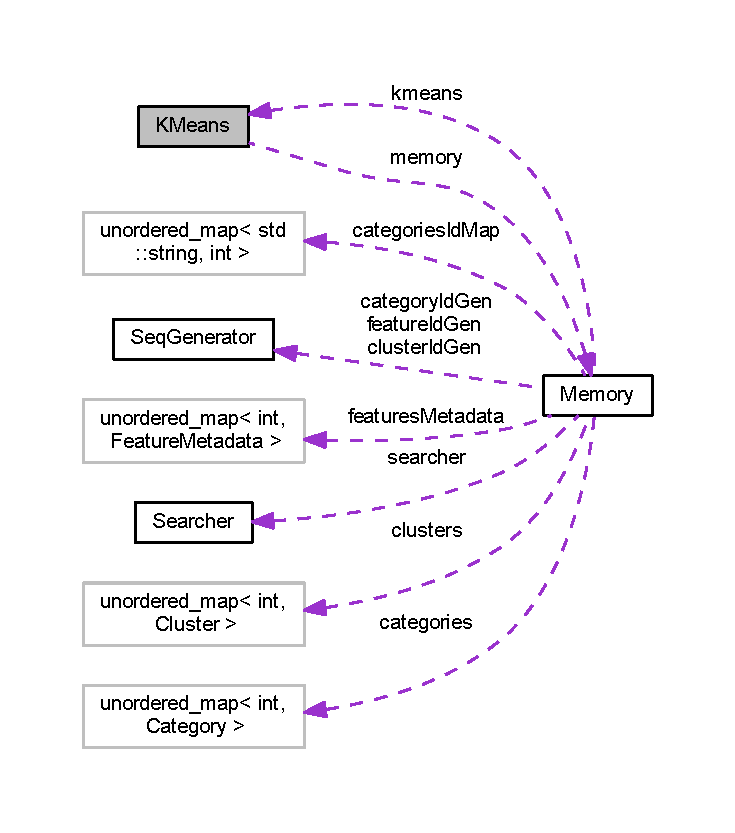
\includegraphics[width=350pt]{class_k_means__coll__graph}
\end{center}
\end{figure}
\subsection*{Public Member Functions}
\begin{DoxyCompactItemize}
\item 
\hyperlink{class_k_means_aa5756bdbeb9251ceb6ee216750f03768}{K\+Means} (int \hyperlink{class_k_means_a605becae019372330541541fec4ecfe5}{max\+Iters}=10)
\item 
void \hyperlink{class_k_means_ac3cd603b2f690e166fb860d5869280e4}{init} (\hyperlink{class_memory}{Memory} \&\hyperlink{class_k_means_af11af5cfa79ac50307a580839d36deef}{memory})
\item 
void \hyperlink{class_k_means_a464d883306ac4e2651eb435207d7b9f5}{update} ()
\item 
void \hyperlink{class_k_means_a8ca0d91448c1e9768808c21fee341e11}{assign} (std\+::vector$<$ int $>$ \&feats\+Idx, int assign\+Cluster=-\/1)
\item 
void \hyperlink{class_k_means_a24391c53c50d73c3c7bab0dabacaeca7}{assign\+Features} (std\+::vector$<$ int $>$ \&feats\+Idx, int \&assign\+Cluster, bool up\+Centroids=true, int max\+Its=1)
\item 
bool \hyperlink{class_k_means_a7aeb5bd10c7faf177955cafab9e55281}{assign\+To\+Clusters} (pcl\+::\+Point\+Cloud$<$ pcl\+::\+Histogram$<$ 153 $>$ $>$\+::Ptr \&centroids, std\+::vector$<$ int $>$ \&mapper, unordered\+\_\+map$<$ int, int $>$ \&rev\+Mapper, \hyperlink{class_feature_metadata}{Feature\+Metadata} \&feat\+Metadata, const int \&feat\+Idx, int k, bool \&up\+Centroids, int \&assign\+Cluster, int \&p\+Cluster, int \&n\+Cluster)
\item 
void \hyperlink{class_k_means_a3da2ed78f2e7b11c67e405fccdda86b7}{find\+Nearest\+Point} (const pcl\+::\+Point\+Cloud$<$ pcl\+::\+Histogram$<$ 153 $>$ $>$\+::Ptr \&points, const pcl\+::\+Histogram$<$ 153 $>$ \&point, std\+::vector$<$ int $>$ \&k\+Indices, std\+::vector$<$ float $>$ \&k\+Sqr\+Distances, int knn)
\item 
void \hyperlink{class_k_means_ad798e3546155a9f694a4be22331e25e7}{recompute\+Centroids} ()
\item 
void \hyperlink{class_k_means_ad4598c662956fc8b224a287f0c2c9ea0}{get\+Centroids} (pcl\+::\+Point\+Cloud$<$ pcl\+::\+Histogram$<$ 153 $>$ $>$\+::Ptr \&centroids, std\+::vector$<$ int $>$ \&mapper, unordered\+\_\+map$<$ int, int $>$ \&rev\+Mapper)
\item 
void \hyperlink{class_k_means_af8f2b01669d61b4093de2854cfe0a935}{check\+Clusters\+Validity} (vector$<$ int $>$ \&touched\+Clusters)
\item 
void \hyperlink{class_k_means_a957725688440a070083e9fcb0f017ce9}{check\+Validity} ()
\item 
void \hyperlink{class_k_means_afd33eafb625ca716c5f808923fb7215e}{split\+Cluster} (int \&cluster\+Id, vector$<$ int $>$ \&touched\+Clusters)
\item 
void \hyperlink{class_k_means_a8e1b5e817bfd073ae331c8ebc3dfb134}{merge\+Clusters} (int \&l\+Cluster\+Id, int \&r\+Cluster\+Id, vector$<$ int $>$ \&touched\+Clusters)
\item 
void \hyperlink{class_k_means_a0004047b206790fee820d57e4b76e9c6}{clean\+Degenerate\+Cluster} (int \&cluster\+Id)
\item 
void \hyperlink{class_k_means_a127c22c2118c8ac22b84a3d2fe01dbf2}{clean\+Empty\+Clusters} (vector$<$ int $>$ \&clusters)
\item 
bool \hyperlink{class_k_means_ac934340bd9baf49360e5cf951f7f6ccb}{check\+Split\+Conditions} (\hyperlink{class_wss_bag}{Wss\+Bag} \&cluster\+Meta)
\item 
bool \hyperlink{class_k_means_a6fd3c45341b534c0ee08bb1ef57ed0d6}{check\+Merge\+Conditions} (\hyperlink{class_wss_bag}{Wss\+Bag} \&cluster\+Meta)
\item 
bool \hyperlink{class_k_means_a58eecd073218a14075ade361a7858563}{check\+Degenerate} (\hyperlink{class_wss_bag}{Wss\+Bag} \&cluster\+Meta)
\item 
int \hyperlink{class_k_means_a280557e55db230a66b5f89c284c88310}{find\+Cluster\+To\+Merge} (vector$<$ pair$<$ int, \hyperlink{class_wss_bag}{Wss\+Bag} $>$ $>$ \&clusters\+Wss, int \&curr\+Ind)
\end{DoxyCompactItemize}
\subsection*{Protected Attributes}
\begin{DoxyCompactItemize}
\item 
int \hyperlink{class_k_means_a605becae019372330541541fec4ecfe5}{max\+Iters}
\item 
int \hyperlink{class_k_means_aa0fdafa4937a817dd15c182ce0c049fe}{max\+Check\+Iters}
\item 
\hyperlink{class_memory}{Memory} $\ast$ \hyperlink{class_k_means_af11af5cfa79ac50307a580839d36deef}{memory}
\item 
float \hyperlink{class_k_means_a95c0e524c7f084ce5a1202d5d6670f45}{wss\+Thresh\+For\+Split}
\item 
int \hyperlink{class_k_means_af056c5370d89a82c2974dfc822624cf0}{min\+Split\+Cluster\+Size}
\item 
int \hyperlink{class_k_means_a99dbe7fd9c440484f54d2f0c2e7bc181}{max\+Split\+Cluster\+Size}
\item 
float \hyperlink{class_k_means_ab002dc02ca5ee154ca56b926a06338d7}{wss\+Thresh\+For\+Merge}
\item 
float \hyperlink{class_k_means_af7004e76ea22f687b4066644a37bf8c9}{bss\+Thresh\+For\+Merge}
\item 
int \hyperlink{class_k_means_a50600403065d0f967e8f2cfdcf6366e8}{degenerate\+Cluster\+Size}
\end{DoxyCompactItemize}


\subsection{Detailed Description}
A custom implementation of Kmeans. 

The number of clusters is dynamic, i.\+e., there can be merge and split of clusters. 

Definition at line 23 of file kmeans.\+h.



\subsection{Constructor \& Destructor Documentation}
\mbox{\Hypertarget{class_k_means_aa5756bdbeb9251ceb6ee216750f03768}\label{class_k_means_aa5756bdbeb9251ceb6ee216750f03768}} 
\index{K\+Means@{K\+Means}!K\+Means@{K\+Means}}
\index{K\+Means@{K\+Means}!K\+Means@{K\+Means}}
\subsubsection{\texorpdfstring{K\+Means()}{KMeans()}}
{\footnotesize\ttfamily K\+Means\+::\+K\+Means (\begin{DoxyParamCaption}\item[{int}]{max\+Iters = {\ttfamily 10} }\end{DoxyParamCaption})}

Constructor 
\begin{DoxyParams}[1]{Parameters}
\mbox{\tt in}  & {\em max\+Iters} & the maximum number of iterations in case convergence can not be achieved \\
\hline
\mbox{\tt in}  & {\em split\+Thresh} & The W\+SS (Within Sum of Squares) threshold to consider splitting a cluster \\
\hline
\mbox{\tt in}  & {\em merge\+Thresh} & The W\+SS (Within Sum of Squares) threshold to consider merging 2 clusters \\
\hline
\mbox{\tt in}  & {\em bss\+Thresh} & The bss threshold \\
\hline
\mbox{\tt in}  & {\em wtss\+Thresh} & The W\+S\+S/\+T\+SS ratio threshold \\
\hline
\mbox{\tt in}  & {\em wtss\+Improve\+Thresh} & The improvement check threshold \\
\hline
\end{DoxyParams}


Definition at line 26 of file kmeans.\+cpp.



\subsection{Member Function Documentation}
\mbox{\Hypertarget{class_k_means_a8ca0d91448c1e9768808c21fee341e11}\label{class_k_means_a8ca0d91448c1e9768808c21fee341e11}} 
\index{K\+Means@{K\+Means}!assign@{assign}}
\index{assign@{assign}!K\+Means@{K\+Means}}
\subsubsection{\texorpdfstring{assign()}{assign()}}
{\footnotesize\ttfamily void K\+Means\+::assign (\begin{DoxyParamCaption}\item[{std\+::vector$<$ int $>$ \&}]{feats\+Idx,  }\item[{int}]{assign\+Cluster = {\ttfamily -\/1} }\end{DoxyParamCaption})}

Assign features to clusters one at a time in a streaming fashion


\begin{DoxyParams}[1]{Parameters}
\mbox{\tt in}  & {\em feats\+Idx} & the keys (indices) of the features \\
\hline
\mbox{\tt in}  & {\em assign\+Cluster} & flag controlling wether features should be assiged to a specific cluster or not \\
\hline
\end{DoxyParams}


Definition at line 110 of file kmeans.\+cpp.

\mbox{\Hypertarget{class_k_means_a24391c53c50d73c3c7bab0dabacaeca7}\label{class_k_means_a24391c53c50d73c3c7bab0dabacaeca7}} 
\index{K\+Means@{K\+Means}!assign\+Features@{assign\+Features}}
\index{assign\+Features@{assign\+Features}!K\+Means@{K\+Means}}
\subsubsection{\texorpdfstring{assign\+Features()}{assignFeatures()}}
{\footnotesize\ttfamily void K\+Means\+::assign\+Features (\begin{DoxyParamCaption}\item[{std\+::vector$<$ int $>$ \&}]{feats\+Idx,  }\item[{int \&}]{assign\+Cluster,  }\item[{bool}]{up\+Centroids = {\ttfamily true},  }\item[{int}]{max\+Its = {\ttfamily 1} }\end{DoxyParamCaption})}

Assign features to clusters one at a time in a streaming fashion (called inside assign)


\begin{DoxyParams}[1]{Parameters}
\mbox{\tt in}  & {\em feats\+Idx} & the keys (indices) of the features \\
\hline
\mbox{\tt in}  & {\em assign\+Cluster} & the identifier of the assignment cluster \\
\hline
\mbox{\tt in}  & {\em up\+Centroids} & flag controlling wether the centroids should be updated or not upon each feature assignment \\
\hline
\mbox{\tt in}  & {\em max\+Its} & the number of times to run the assignment (defaults to 1) \\
\hline
\end{DoxyParams}


Definition at line 131 of file kmeans.\+cpp.

\mbox{\Hypertarget{class_k_means_a7aeb5bd10c7faf177955cafab9e55281}\label{class_k_means_a7aeb5bd10c7faf177955cafab9e55281}} 
\index{K\+Means@{K\+Means}!assign\+To\+Clusters@{assign\+To\+Clusters}}
\index{assign\+To\+Clusters@{assign\+To\+Clusters}!K\+Means@{K\+Means}}
\subsubsection{\texorpdfstring{assign\+To\+Clusters()}{assignToClusters()}}
{\footnotesize\ttfamily bool K\+Means\+::assign\+To\+Clusters (\begin{DoxyParamCaption}\item[{pcl\+::\+Point\+Cloud$<$ pcl\+::\+Histogram$<$ 153 $>$ $>$\+::Ptr \&}]{centroids,  }\item[{std\+::vector$<$ int $>$ \&}]{mapper,  }\item[{unordered\+\_\+map$<$ int, int $>$ \&}]{rev\+Mapper,  }\item[{\hyperlink{class_feature_metadata}{Feature\+Metadata} \&}]{feat\+Metadata,  }\item[{const int \&}]{feat\+Idx,  }\item[{int}]{k,  }\item[{bool \&}]{up\+Centroids,  }\item[{int \&}]{assign\+Cluster,  }\item[{int \&}]{p\+Cluster,  }\item[{int \&}]{n\+Cluster }\end{DoxyParamCaption})}

Temporary work around for fit. Used only in a specific situation! This should change! Run the \hyperlink{class_k_means}{K\+Means} algorithm to perform the clustering until convergence or the maximum number of iterations has been reached

For computational performance \hyperlink{class_k_means}{K\+Means} runs only over the features added at each batch of computed features


\begin{DoxyParams}[1]{Parameters}
\mbox{\tt in}  & {\em feats\+Idx} & the keys (indices) of the features Assign the feature specified in feat\+Metadata to the nearest cluster\\
\hline
\mbox{\tt in}  & {\em centroids} & the cenroids of th cluters \\
\hline
\mbox{\tt in}  & {\em mapper} & mapper a structure that maps from the centroids vector indexes to the cluster identifiers \\
\hline
\mbox{\tt in}  & {\em rev\+Mapper} & a structure that maps from the cluster identifiers to the centroids vector indexes \\
\hline
\mbox{\tt in}  & {\em feat\+Metadata} & the feature metadata (contains the feature to be assigned) \\
\hline
\mbox{\tt in}  & {\em feat\+Idx} & the index of the feature in the memory vector \\
\hline
\mbox{\tt in}  & {\em k} & the number of nearest cluster centroids to consider for cluster assignment \\
\hline
\mbox{\tt in}  & {\em up\+Centroids} & if set to true the centroids will be updated after each new assignment \\
\hline
\mbox{\tt in}  & {\em assign\+Cluster} & the identifier of the assignment cluster \\
\hline
\mbox{\tt out}  & {\em p\+Cluster} & the previous cluster assignment (of the feature) \\
\hline
\mbox{\tt out}  & {\em n\+Cluster} & the new cluster assignment (of the feature)\\
\hline
\end{DoxyParams}
Returns true if a new assignmnt took place, false otherwise

p.\+s. If an assignment cluster (assgn\+Cluster) is specified, then the features are assigned to that cluster. If no assignment cluster is specified (assgn\+Cluster = -\/1), then the features are assigned to the nearest cluster 

Definition at line 192 of file kmeans.\+cpp.

\mbox{\Hypertarget{class_k_means_af8f2b01669d61b4093de2854cfe0a935}\label{class_k_means_af8f2b01669d61b4093de2854cfe0a935}} 
\index{K\+Means@{K\+Means}!check\+Clusters\+Validity@{check\+Clusters\+Validity}}
\index{check\+Clusters\+Validity@{check\+Clusters\+Validity}!K\+Means@{K\+Means}}
\subsubsection{\texorpdfstring{check\+Clusters\+Validity()}{checkClustersValidity()}}
{\footnotesize\ttfamily void K\+Means\+::check\+Clusters\+Validity (\begin{DoxyParamCaption}\item[{vector$<$ int $>$ \&}]{touched\+Clusters }\end{DoxyParamCaption})}

Check the quality of the clusters


\begin{DoxyParams}[1]{Parameters}
\mbox{\tt out}  & {\em touched\+Clusters} & the list of clusters modified by the checking process \\
\hline
\end{DoxyParams}


Definition at line 477 of file kmeans.\+cpp.

\mbox{\Hypertarget{class_k_means_a58eecd073218a14075ade361a7858563}\label{class_k_means_a58eecd073218a14075ade361a7858563}} 
\index{K\+Means@{K\+Means}!check\+Degenerate@{check\+Degenerate}}
\index{check\+Degenerate@{check\+Degenerate}!K\+Means@{K\+Means}}
\subsubsection{\texorpdfstring{check\+Degenerate()}{checkDegenerate()}}
{\footnotesize\ttfamily bool K\+Means\+::check\+Degenerate (\begin{DoxyParamCaption}\item[{\hyperlink{class_wss_bag}{Wss\+Bag} \&}]{cluster\+Meta }\end{DoxyParamCaption})}



Definition at line 525 of file kmeans.\+cpp.

\mbox{\Hypertarget{class_k_means_a6fd3c45341b534c0ee08bb1ef57ed0d6}\label{class_k_means_a6fd3c45341b534c0ee08bb1ef57ed0d6}} 
\index{K\+Means@{K\+Means}!check\+Merge\+Conditions@{check\+Merge\+Conditions}}
\index{check\+Merge\+Conditions@{check\+Merge\+Conditions}!K\+Means@{K\+Means}}
\subsubsection{\texorpdfstring{check\+Merge\+Conditions()}{checkMergeConditions()}}
{\footnotesize\ttfamily bool K\+Means\+::check\+Merge\+Conditions (\begin{DoxyParamCaption}\item[{\hyperlink{class_wss_bag}{Wss\+Bag} \&}]{cluster\+Meta }\end{DoxyParamCaption})}

Check for if the specified cluster fits the conditions to be merged


\begin{DoxyParams}[1]{Parameters}
\mbox{\tt in}  & {\em cluster\+Meta} & metadata concerning th cluster to be verified against the merging conditions \\
\hline
\end{DoxyParams}


Definition at line 554 of file kmeans.\+cpp.

\mbox{\Hypertarget{class_k_means_ac934340bd9baf49360e5cf951f7f6ccb}\label{class_k_means_ac934340bd9baf49360e5cf951f7f6ccb}} 
\index{K\+Means@{K\+Means}!check\+Split\+Conditions@{check\+Split\+Conditions}}
\index{check\+Split\+Conditions@{check\+Split\+Conditions}!K\+Means@{K\+Means}}
\subsubsection{\texorpdfstring{check\+Split\+Conditions()}{checkSplitConditions()}}
{\footnotesize\ttfamily bool K\+Means\+::check\+Split\+Conditions (\begin{DoxyParamCaption}\item[{\hyperlink{class_wss_bag}{Wss\+Bag} \&}]{cluster\+Meta }\end{DoxyParamCaption})}

Check for if the specified cluster fits the conditions to be splitted


\begin{DoxyParams}[1]{Parameters}
\mbox{\tt in}  & {\em cluster\+Meta} & metadata concerning th cluster to be verified against the splitting conditions \\
\hline
\end{DoxyParams}


Definition at line 535 of file kmeans.\+cpp.

\mbox{\Hypertarget{class_k_means_a957725688440a070083e9fcb0f017ce9}\label{class_k_means_a957725688440a070083e9fcb0f017ce9}} 
\index{K\+Means@{K\+Means}!check\+Validity@{check\+Validity}}
\index{check\+Validity@{check\+Validity}!K\+Means@{K\+Means}}
\subsubsection{\texorpdfstring{check\+Validity()}{checkValidity()}}
{\footnotesize\ttfamily void K\+Means\+::check\+Validity (\begin{DoxyParamCaption}{ }\end{DoxyParamCaption})}



Definition at line 371 of file kmeans.\+cpp.

\mbox{\Hypertarget{class_k_means_a0004047b206790fee820d57e4b76e9c6}\label{class_k_means_a0004047b206790fee820d57e4b76e9c6}} 
\index{K\+Means@{K\+Means}!clean\+Degenerate\+Cluster@{clean\+Degenerate\+Cluster}}
\index{clean\+Degenerate\+Cluster@{clean\+Degenerate\+Cluster}!K\+Means@{K\+Means}}
\subsubsection{\texorpdfstring{clean\+Degenerate\+Cluster()}{cleanDegenerateCluster()}}
{\footnotesize\ttfamily void K\+Means\+::clean\+Degenerate\+Cluster (\begin{DoxyParamCaption}\item[{int \&}]{cluster\+Id }\end{DoxyParamCaption})}



Definition at line 723 of file kmeans.\+cpp.

\mbox{\Hypertarget{class_k_means_a127c22c2118c8ac22b84a3d2fe01dbf2}\label{class_k_means_a127c22c2118c8ac22b84a3d2fe01dbf2}} 
\index{K\+Means@{K\+Means}!clean\+Empty\+Clusters@{clean\+Empty\+Clusters}}
\index{clean\+Empty\+Clusters@{clean\+Empty\+Clusters}!K\+Means@{K\+Means}}
\subsubsection{\texorpdfstring{clean\+Empty\+Clusters()}{cleanEmptyClusters()}}
{\footnotesize\ttfamily void K\+Means\+::clean\+Empty\+Clusters (\begin{DoxyParamCaption}\item[{vector$<$ int $>$ \&}]{clusters }\end{DoxyParamCaption})}

Removes empty clusters from the clusters list


\begin{DoxyParams}[1]{Parameters}
\mbox{\tt in}  & {\em clusters} & metadata the list of candidate clusters to consider for removal \\
\hline
\end{DoxyParams}


Definition at line 595 of file kmeans.\+cpp.

\mbox{\Hypertarget{class_k_means_a280557e55db230a66b5f89c284c88310}\label{class_k_means_a280557e55db230a66b5f89c284c88310}} 
\index{K\+Means@{K\+Means}!find\+Cluster\+To\+Merge@{find\+Cluster\+To\+Merge}}
\index{find\+Cluster\+To\+Merge@{find\+Cluster\+To\+Merge}!K\+Means@{K\+Means}}
\subsubsection{\texorpdfstring{find\+Cluster\+To\+Merge()}{findClusterToMerge()}}
{\footnotesize\ttfamily int K\+Means\+::find\+Cluster\+To\+Merge (\begin{DoxyParamCaption}\item[{vector$<$ pair$<$ int, \hyperlink{class_wss_bag}{Wss\+Bag} $>$ $>$ \&}]{clusters\+Wss,  }\item[{int \&}]{curr\+Ind }\end{DoxyParamCaption})}

Finds a suitable cluster to perform a merge operation with the specified cluster


\begin{DoxyParams}[1]{Parameters}
\mbox{\tt in}  & {\em clusters\+Wss} & the list of candidate clusters \\
\hline
\mbox{\tt in}  & {\em curr\+Ind} & the index specifying the current cluster\\
\hline
\end{DoxyParams}
Returns the identifier of the cluster if one could be found, -\/1 otherwise 

Definition at line 567 of file kmeans.\+cpp.

\mbox{\Hypertarget{class_k_means_a3da2ed78f2e7b11c67e405fccdda86b7}\label{class_k_means_a3da2ed78f2e7b11c67e405fccdda86b7}} 
\index{K\+Means@{K\+Means}!find\+Nearest\+Point@{find\+Nearest\+Point}}
\index{find\+Nearest\+Point@{find\+Nearest\+Point}!K\+Means@{K\+Means}}
\subsubsection{\texorpdfstring{find\+Nearest\+Point()}{findNearestPoint()}}
{\footnotesize\ttfamily void K\+Means\+::find\+Nearest\+Point (\begin{DoxyParamCaption}\item[{const pcl\+::\+Point\+Cloud$<$ pcl\+::\+Histogram$<$ 153 $>$ $>$\+::Ptr \&}]{points,  }\item[{const pcl\+::\+Histogram$<$ 153 $>$ \&}]{point,  }\item[{std\+::vector$<$ int $>$ \&}]{k\+Indices,  }\item[{std\+::vector$<$ float $>$ \&}]{k\+Sqr\+Distances,  }\item[{int}]{knn }\end{DoxyParamCaption})}

Find the nearest point amongst the given points to the specified point


\begin{DoxyParams}[1]{Parameters}
\mbox{\tt in}  & {\em points} & the points to search in for the closest point \\
\hline
\mbox{\tt in}  & {\em point} & the point to compare to the points \\
\hline
\mbox{\tt in}  & {\em k\+Indices} & returns the indices of the knn nearest centroids \\
\hline
\mbox{\tt in}  & {\em k\+Sqr\+Distances} & returns the squared distances to the centroids \\
\hline
\mbox{\tt in}  & {\em knn} & the number of nearest centroids to search for \\
\hline
\end{DoxyParams}


Definition at line 363 of file kmeans.\+cpp.

\mbox{\Hypertarget{class_k_means_ad4598c662956fc8b224a287f0c2c9ea0}\label{class_k_means_ad4598c662956fc8b224a287f0c2c9ea0}} 
\index{K\+Means@{K\+Means}!get\+Centroids@{get\+Centroids}}
\index{get\+Centroids@{get\+Centroids}!K\+Means@{K\+Means}}
\subsubsection{\texorpdfstring{get\+Centroids()}{getCentroids()}}
{\footnotesize\ttfamily void K\+Means\+::get\+Centroids (\begin{DoxyParamCaption}\item[{pcl\+::\+Point\+Cloud$<$ pcl\+::\+Histogram$<$ 153 $>$ $>$\+::Ptr \&}]{centroids,  }\item[{std\+::vector$<$ int $>$ \&}]{mapper,  }\item[{unordered\+\_\+map$<$ int, int $>$ \&}]{rev\+Mapper }\end{DoxyParamCaption})}

Retrieve the cluster centroids stored in memory. If no clustera are defined yet, a cluster is created and a random point in memory is taken as its centroid


\begin{DoxyParams}[1]{Parameters}
\mbox{\tt out}  & {\em centroids} & the centroids of the clusters \\
\hline
\mbox{\tt out}  & {\em mapper} & a structure that maps from the centroids vector indexes to the cluster identifiers \\
\hline
\mbox{\tt out}  & {\em rev\+Mapper} & a structure that maps from the cluster identifiers to the centroids vector indexes \\
\hline
\end{DoxyParams}


Definition at line 265 of file kmeans.\+cpp.

\mbox{\Hypertarget{class_k_means_ac3cd603b2f690e166fb860d5869280e4}\label{class_k_means_ac3cd603b2f690e166fb860d5869280e4}} 
\index{K\+Means@{K\+Means}!init@{init}}
\index{init@{init}!K\+Means@{K\+Means}}
\subsubsection{\texorpdfstring{init()}{init()}}
{\footnotesize\ttfamily void K\+Means\+::init (\begin{DoxyParamCaption}\item[{\hyperlink{class_memory}{Memory} \&}]{memory }\end{DoxyParamCaption})}

Initialize K\+M\+Eans by setting the internal reference (pointer) to the memory structure 

Definition at line 38 of file kmeans.\+cpp.

\mbox{\Hypertarget{class_k_means_a8e1b5e817bfd073ae331c8ebc3dfb134}\label{class_k_means_a8e1b5e817bfd073ae331c8ebc3dfb134}} 
\index{K\+Means@{K\+Means}!merge\+Clusters@{merge\+Clusters}}
\index{merge\+Clusters@{merge\+Clusters}!K\+Means@{K\+Means}}
\subsubsection{\texorpdfstring{merge\+Clusters()}{mergeClusters()}}
{\footnotesize\ttfamily void K\+Means\+::merge\+Clusters (\begin{DoxyParamCaption}\item[{int \&}]{l\+Cluster\+Id,  }\item[{int \&}]{r\+Cluster\+Id,  }\item[{vector$<$ int $>$ \&}]{touched\+Clusters }\end{DoxyParamCaption})}

Perform a merge operation between the specified clusters


\begin{DoxyParams}[1]{Parameters}
\mbox{\tt in}  & {\em l\+Cluster\+Id} & the first cluster identifier to merge \\
\hline
\mbox{\tt in}  & {\em r\+Cluster\+Id} & the second cluster identifier to merge \\
\hline
\mbox{\tt out}  & {\em touched\+Clusters} & the list of clusters modified by the checking process \\
\hline
\end{DoxyParams}


Definition at line 681 of file kmeans.\+cpp.

\mbox{\Hypertarget{class_k_means_ad798e3546155a9f694a4be22331e25e7}\label{class_k_means_ad798e3546155a9f694a4be22331e25e7}} 
\index{K\+Means@{K\+Means}!recompute\+Centroids@{recompute\+Centroids}}
\index{recompute\+Centroids@{recompute\+Centroids}!K\+Means@{K\+Means}}
\subsubsection{\texorpdfstring{recompute\+Centroids()}{recomputeCentroids()}}
{\footnotesize\ttfamily void K\+Means\+::recompute\+Centroids (\begin{DoxyParamCaption}{ }\end{DoxyParamCaption})}

Recomputes all cluster centroids 

Definition at line 335 of file kmeans.\+cpp.

\mbox{\Hypertarget{class_k_means_afd33eafb625ca716c5f808923fb7215e}\label{class_k_means_afd33eafb625ca716c5f808923fb7215e}} 
\index{K\+Means@{K\+Means}!split\+Cluster@{split\+Cluster}}
\index{split\+Cluster@{split\+Cluster}!K\+Means@{K\+Means}}
\subsubsection{\texorpdfstring{split\+Cluster()}{splitCluster()}}
{\footnotesize\ttfamily void K\+Means\+::split\+Cluster (\begin{DoxyParamCaption}\item[{int \&}]{cluster\+Id,  }\item[{vector$<$ int $>$ \&}]{touched\+Clusters }\end{DoxyParamCaption})}

Perform a split operation on the specified cluster

After the split, a fit must be performed in order to stabalize the newly created clusters


\begin{DoxyParams}[1]{Parameters}
\mbox{\tt in}  & {\em cluster\+Id} & the cluster identifier \\
\hline
\mbox{\tt out}  & {\em touched\+Clusters} & the list of clusters modified by the checking process \\
\hline
\end{DoxyParams}


Definition at line 604 of file kmeans.\+cpp.

\mbox{\Hypertarget{class_k_means_a464d883306ac4e2651eb435207d7b9f5}\label{class_k_means_a464d883306ac4e2651eb435207d7b9f5}} 
\index{K\+Means@{K\+Means}!update@{update}}
\index{update@{update}!K\+Means@{K\+Means}}
\subsubsection{\texorpdfstring{update()}{update()}}
{\footnotesize\ttfamily void K\+Means\+::update (\begin{DoxyParamCaption}{ }\end{DoxyParamCaption})}

Update kmeans after forgeting a feature 

Definition at line 43 of file kmeans.\+cpp.



\subsection{Member Data Documentation}
\mbox{\Hypertarget{class_k_means_af7004e76ea22f687b4066644a37bf8c9}\label{class_k_means_af7004e76ea22f687b4066644a37bf8c9}} 
\index{K\+Means@{K\+Means}!bss\+Thresh\+For\+Merge@{bss\+Thresh\+For\+Merge}}
\index{bss\+Thresh\+For\+Merge@{bss\+Thresh\+For\+Merge}!K\+Means@{K\+Means}}
\subsubsection{\texorpdfstring{bss\+Thresh\+For\+Merge}{bssThreshForMerge}}
{\footnotesize\ttfamily float K\+Means\+::bss\+Thresh\+For\+Merge\hspace{0.3cm}{\ttfamily [protected]}}



Definition at line 308 of file kmeans.\+h.

\mbox{\Hypertarget{class_k_means_a50600403065d0f967e8f2cfdcf6366e8}\label{class_k_means_a50600403065d0f967e8f2cfdcf6366e8}} 
\index{K\+Means@{K\+Means}!degenerate\+Cluster\+Size@{degenerate\+Cluster\+Size}}
\index{degenerate\+Cluster\+Size@{degenerate\+Cluster\+Size}!K\+Means@{K\+Means}}
\subsubsection{\texorpdfstring{degenerate\+Cluster\+Size}{degenerateClusterSize}}
{\footnotesize\ttfamily int K\+Means\+::degenerate\+Cluster\+Size\hspace{0.3cm}{\ttfamily [protected]}}



Definition at line 311 of file kmeans.\+h.

\mbox{\Hypertarget{class_k_means_aa0fdafa4937a817dd15c182ce0c049fe}\label{class_k_means_aa0fdafa4937a817dd15c182ce0c049fe}} 
\index{K\+Means@{K\+Means}!max\+Check\+Iters@{max\+Check\+Iters}}
\index{max\+Check\+Iters@{max\+Check\+Iters}!K\+Means@{K\+Means}}
\subsubsection{\texorpdfstring{max\+Check\+Iters}{maxCheckIters}}
{\footnotesize\ttfamily int K\+Means\+::max\+Check\+Iters\hspace{0.3cm}{\ttfamily [protected]}}

The maximum number of iterations for cluster validity check 

Definition at line 224 of file kmeans.\+h.

\mbox{\Hypertarget{class_k_means_a605becae019372330541541fec4ecfe5}\label{class_k_means_a605becae019372330541541fec4ecfe5}} 
\index{K\+Means@{K\+Means}!max\+Iters@{max\+Iters}}
\index{max\+Iters@{max\+Iters}!K\+Means@{K\+Means}}
\subsubsection{\texorpdfstring{max\+Iters}{maxIters}}
{\footnotesize\ttfamily int K\+Means\+::max\+Iters\hspace{0.3cm}{\ttfamily [protected]}}

The maximum number of iterations 

Definition at line 219 of file kmeans.\+h.

\mbox{\Hypertarget{class_k_means_a99dbe7fd9c440484f54d2f0c2e7bc181}\label{class_k_means_a99dbe7fd9c440484f54d2f0c2e7bc181}} 
\index{K\+Means@{K\+Means}!max\+Split\+Cluster\+Size@{max\+Split\+Cluster\+Size}}
\index{max\+Split\+Cluster\+Size@{max\+Split\+Cluster\+Size}!K\+Means@{K\+Means}}
\subsubsection{\texorpdfstring{max\+Split\+Cluster\+Size}{maxSplitClusterSize}}
{\footnotesize\ttfamily int K\+Means\+::max\+Split\+Cluster\+Size\hspace{0.3cm}{\ttfamily [protected]}}



Definition at line 302 of file kmeans.\+h.

\mbox{\Hypertarget{class_k_means_af11af5cfa79ac50307a580839d36deef}\label{class_k_means_af11af5cfa79ac50307a580839d36deef}} 
\index{K\+Means@{K\+Means}!memory@{memory}}
\index{memory@{memory}!K\+Means@{K\+Means}}
\subsubsection{\texorpdfstring{memory}{memory}}
{\footnotesize\ttfamily \hyperlink{class_memory}{Memory}$\ast$ K\+Means\+::memory\hspace{0.3cm}{\ttfamily [protected]}}

Pointer to the memory structure holding the features 

Definition at line 229 of file kmeans.\+h.

\mbox{\Hypertarget{class_k_means_af056c5370d89a82c2974dfc822624cf0}\label{class_k_means_af056c5370d89a82c2974dfc822624cf0}} 
\index{K\+Means@{K\+Means}!min\+Split\+Cluster\+Size@{min\+Split\+Cluster\+Size}}
\index{min\+Split\+Cluster\+Size@{min\+Split\+Cluster\+Size}!K\+Means@{K\+Means}}
\subsubsection{\texorpdfstring{min\+Split\+Cluster\+Size}{minSplitClusterSize}}
{\footnotesize\ttfamily int K\+Means\+::min\+Split\+Cluster\+Size\hspace{0.3cm}{\ttfamily [protected]}}



Definition at line 298 of file kmeans.\+h.

\mbox{\Hypertarget{class_k_means_ab002dc02ca5ee154ca56b926a06338d7}\label{class_k_means_ab002dc02ca5ee154ca56b926a06338d7}} 
\index{K\+Means@{K\+Means}!wss\+Thresh\+For\+Merge@{wss\+Thresh\+For\+Merge}}
\index{wss\+Thresh\+For\+Merge@{wss\+Thresh\+For\+Merge}!K\+Means@{K\+Means}}
\subsubsection{\texorpdfstring{wss\+Thresh\+For\+Merge}{wssThreshForMerge}}
{\footnotesize\ttfamily float K\+Means\+::wss\+Thresh\+For\+Merge\hspace{0.3cm}{\ttfamily [protected]}}



Definition at line 305 of file kmeans.\+h.

\mbox{\Hypertarget{class_k_means_a95c0e524c7f084ce5a1202d5d6670f45}\label{class_k_means_a95c0e524c7f084ce5a1202d5d6670f45}} 
\index{K\+Means@{K\+Means}!wss\+Thresh\+For\+Split@{wss\+Thresh\+For\+Split}}
\index{wss\+Thresh\+For\+Split@{wss\+Thresh\+For\+Split}!K\+Means@{K\+Means}}
\subsubsection{\texorpdfstring{wss\+Thresh\+For\+Split}{wssThreshForSplit}}
{\footnotesize\ttfamily float K\+Means\+::wss\+Thresh\+For\+Split\hspace{0.3cm}{\ttfamily [protected]}}

Thresholds The W\+S\+S/\+T\+SS ratio

Holds the last W\+S\+S/\+T\+SS ratio computed to check cluster quality The W\+SS (Within Sum of Squares) threshold to consider splitting a cluster

The cluster will be consider for spliting if its W\+SS measure is above this value

y default it is innitialized to 2.\+0f The W\+SS (Within Sum of Squares) threshold to consider merging 2 clusters

The cluster will be consider for merging if its W\+SS measure is below this value

By default it is innitialized to 1.\+0f The bss threshold

Used to check clustering quality. If the B\+SS measure between 2 clusters falls below this threshold, then the cluster will be considered for merging (in case their individual W\+SS measures are also below the \textquotesingle{}merge\+Thresh\textquotesingle{} value)

By default it is innitialized to 1.\+0f The W\+S\+S/\+T\+SS ratio threshold

Used to check clustering quality. A value close to or below 0.\+2 means good clustering quality. A value above is an indication of non-\/optimum clustering quality

By default it is innitialized to 0.\+2f The improvement check threshold

If only a small improvement would be achieved, then no attempt to improve clustering quality is performed, and is delayed until a bigger improvement can be achieved

By default it is innitialized to 0.\+1f 

Definition at line 294 of file kmeans.\+h.



The documentation for this class was generated from the following files\+:\begin{DoxyCompactItemize}
\item 
H\+:/\+M\+E\+I/sistemas inteligentes/tp2/\+S\+I\+\_\+\+C\+O\+D\+E/include/\hyperlink{kmeans_8h}{kmeans.\+h}\item 
H\+:/\+M\+E\+I/sistemas inteligentes/tp2/\+S\+I\+\_\+\+C\+O\+D\+E/src/\hyperlink{kmeans_8cpp}{kmeans.\+cpp}\end{DoxyCompactItemize}

\hypertarget{structlinux__dirent}{}\section{linux\+\_\+dirent Struct Reference}
\label{structlinux__dirent}\index{linux\+\_\+dirent@{linux\+\_\+dirent}}


{\ttfamily \#include $<$include.\+h$>$}

\subsection*{Public Attributes}
\begin{DoxyCompactItemize}
\item 
long \hyperlink{structlinux__dirent_a7ed8ec01b550ca3567776b0be32e8af8}{d\+\_\+ino}
\item 
off\+\_\+t \hyperlink{structlinux__dirent_a8c685abf351d3f31a8dd119e4a775078}{d\+\_\+off}
\item 
unsigned short \hyperlink{structlinux__dirent_a42ba867e75bb4fbf7cae374bc58ee91a}{d\+\_\+reclen}
\item 
char \hyperlink{structlinux__dirent_a7e12cde71271d11545975d19b13200fa}{d\+\_\+name} \mbox{[}$\,$\mbox{]}
\end{DoxyCompactItemize}


\subsection{Detailed Description}


Definition at line 60 of file include.\+h.



\subsection{Member Data Documentation}
\mbox{\Hypertarget{structlinux__dirent_a7ed8ec01b550ca3567776b0be32e8af8}\label{structlinux__dirent_a7ed8ec01b550ca3567776b0be32e8af8}} 
\index{linux\+\_\+dirent@{linux\+\_\+dirent}!d\+\_\+ino@{d\+\_\+ino}}
\index{d\+\_\+ino@{d\+\_\+ino}!linux\+\_\+dirent@{linux\+\_\+dirent}}
\subsubsection{\texorpdfstring{d\+\_\+ino}{d\_ino}}
{\footnotesize\ttfamily long linux\+\_\+dirent\+::d\+\_\+ino}



Definition at line 61 of file include.\+h.

\mbox{\Hypertarget{structlinux__dirent_a7e12cde71271d11545975d19b13200fa}\label{structlinux__dirent_a7e12cde71271d11545975d19b13200fa}} 
\index{linux\+\_\+dirent@{linux\+\_\+dirent}!d\+\_\+name@{d\+\_\+name}}
\index{d\+\_\+name@{d\+\_\+name}!linux\+\_\+dirent@{linux\+\_\+dirent}}
\subsubsection{\texorpdfstring{d\+\_\+name}{d\_name}}
{\footnotesize\ttfamily char linux\+\_\+dirent\+::d\+\_\+name\mbox{[}$\,$\mbox{]}}



Definition at line 64 of file include.\+h.

\mbox{\Hypertarget{structlinux__dirent_a8c685abf351d3f31a8dd119e4a775078}\label{structlinux__dirent_a8c685abf351d3f31a8dd119e4a775078}} 
\index{linux\+\_\+dirent@{linux\+\_\+dirent}!d\+\_\+off@{d\+\_\+off}}
\index{d\+\_\+off@{d\+\_\+off}!linux\+\_\+dirent@{linux\+\_\+dirent}}
\subsubsection{\texorpdfstring{d\+\_\+off}{d\_off}}
{\footnotesize\ttfamily off\+\_\+t linux\+\_\+dirent\+::d\+\_\+off}



Definition at line 62 of file include.\+h.

\mbox{\Hypertarget{structlinux__dirent_a42ba867e75bb4fbf7cae374bc58ee91a}\label{structlinux__dirent_a42ba867e75bb4fbf7cae374bc58ee91a}} 
\index{linux\+\_\+dirent@{linux\+\_\+dirent}!d\+\_\+reclen@{d\+\_\+reclen}}
\index{d\+\_\+reclen@{d\+\_\+reclen}!linux\+\_\+dirent@{linux\+\_\+dirent}}
\subsubsection{\texorpdfstring{d\+\_\+reclen}{d\_reclen}}
{\footnotesize\ttfamily unsigned short linux\+\_\+dirent\+::d\+\_\+reclen}



Definition at line 63 of file include.\+h.



The documentation for this struct was generated from the following file\+:\begin{DoxyCompactItemize}
\item 
H\+:/\+M\+E\+I/sistemas inteligentes/tp2/\+S\+I\+\_\+\+C\+O\+D\+E/include/\hyperlink{include_8h}{include.\+h}\end{DoxyCompactItemize}

\hypertarget{class_measure}{}\section{Measure Class Reference}
\label{class_measure}\index{Measure@{Measure}}


A class used to measure the performance of the application assigning object views to categories. Use to hold the results for a specific category.  




{\ttfamily \#include $<$Measure.\+h$>$}

\subsection*{Public Member Functions}
\begin{DoxyCompactItemize}
\item 
\hyperlink{class_measure_ab55c93d6121f43c91a337fb7bcd26825}{Measure} ()
\item 
int \& \hyperlink{class_measure_a28c4d8877916c477d2e3003d3f467ca2}{get\+TP} ()
\item 
int \& \hyperlink{class_measure_a68c038fe576017b5d3ce00895dc0aeb5}{get\+FP} ()
\item 
int \& \hyperlink{class_measure_a9b2213f1dd9fd63e64629ecbb8ecce35}{get\+FN} ()
\item 
void \hyperlink{class_measure_a163284f13b6b79ba19f7db571365c7e1}{add\+TP} ()
\item 
void \hyperlink{class_measure_ae3b5b1f8db1a660dd55495bcc69d2a3d}{add\+FP} ()
\item 
void \hyperlink{class_measure_adfac0ce9647ed61b6fdfa6c81b1e5971}{add\+FN} ()
\item 
double \hyperlink{class_measure_a2cac1a29c5ae012b810499be8d301753}{precision} ()
\item 
double \hyperlink{class_measure_afb7cbc9872452a8ce1f78e6f0661daa0}{recall} ()
\end{DoxyCompactItemize}
\subsection*{Protected Attributes}
\begin{DoxyCompactItemize}
\item 
int \hyperlink{class_measure_a88e0c0f67850429f30650a2b7e7076aa}{tp}
\item 
int \hyperlink{class_measure_a2f4b9fd7379fc019a8dd276f316eddd7}{fp}
\item 
int \hyperlink{class_measure_ac0e820e813b633be8aa145f415aa81eb}{fn}
\end{DoxyCompactItemize}


\subsection{Detailed Description}
A class used to measure the performance of the application assigning object views to categories. Use to hold the results for a specific category. 

Definition at line 10 of file Measure.\+h.



\subsection{Constructor \& Destructor Documentation}
\mbox{\Hypertarget{class_measure_ab55c93d6121f43c91a337fb7bcd26825}\label{class_measure_ab55c93d6121f43c91a337fb7bcd26825}} 
\index{Measure@{Measure}!Measure@{Measure}}
\index{Measure@{Measure}!Measure@{Measure}}
\subsubsection{\texorpdfstring{Measure()}{Measure()}}
{\footnotesize\ttfamily Measure\+::\+Measure (\begin{DoxyParamCaption}{ }\end{DoxyParamCaption})}

The empty constructor is required when used as the value in a map. 

Definition at line 3 of file Measure.\+cpp.



\subsection{Member Function Documentation}
\mbox{\Hypertarget{class_measure_adfac0ce9647ed61b6fdfa6c81b1e5971}\label{class_measure_adfac0ce9647ed61b6fdfa6c81b1e5971}} 
\index{Measure@{Measure}!add\+FN@{add\+FN}}
\index{add\+FN@{add\+FN}!Measure@{Measure}}
\subsubsection{\texorpdfstring{add\+F\+N()}{addFN()}}
{\footnotesize\ttfamily void Measure\+::add\+FN (\begin{DoxyParamCaption}{ }\end{DoxyParamCaption})\hspace{0.3cm}{\ttfamily [inline]}}

Increments the amount of false negatives. 

Definition at line 73 of file Measure.\+h.

\mbox{\Hypertarget{class_measure_ae3b5b1f8db1a660dd55495bcc69d2a3d}\label{class_measure_ae3b5b1f8db1a660dd55495bcc69d2a3d}} 
\index{Measure@{Measure}!add\+FP@{add\+FP}}
\index{add\+FP@{add\+FP}!Measure@{Measure}}
\subsubsection{\texorpdfstring{add\+F\+P()}{addFP()}}
{\footnotesize\ttfamily void Measure\+::add\+FP (\begin{DoxyParamCaption}{ }\end{DoxyParamCaption})\hspace{0.3cm}{\ttfamily [inline]}}

Increments the amount of false positives. 

Definition at line 66 of file Measure.\+h.

\mbox{\Hypertarget{class_measure_a163284f13b6b79ba19f7db571365c7e1}\label{class_measure_a163284f13b6b79ba19f7db571365c7e1}} 
\index{Measure@{Measure}!add\+TP@{add\+TP}}
\index{add\+TP@{add\+TP}!Measure@{Measure}}
\subsubsection{\texorpdfstring{add\+T\+P()}{addTP()}}
{\footnotesize\ttfamily void Measure\+::add\+TP (\begin{DoxyParamCaption}{ }\end{DoxyParamCaption})\hspace{0.3cm}{\ttfamily [inline]}}

Increments the amount of true positives. 

Definition at line 59 of file Measure.\+h.

\mbox{\Hypertarget{class_measure_a9b2213f1dd9fd63e64629ecbb8ecce35}\label{class_measure_a9b2213f1dd9fd63e64629ecbb8ecce35}} 
\index{Measure@{Measure}!get\+FN@{get\+FN}}
\index{get\+FN@{get\+FN}!Measure@{Measure}}
\subsubsection{\texorpdfstring{get\+F\+N()}{getFN()}}
{\footnotesize\ttfamily int\& Measure\+::get\+FN (\begin{DoxyParamCaption}{ }\end{DoxyParamCaption})\hspace{0.3cm}{\ttfamily [inline]}}

Gets the amount of false negatives. 

Definition at line 52 of file Measure.\+h.

\mbox{\Hypertarget{class_measure_a68c038fe576017b5d3ce00895dc0aeb5}\label{class_measure_a68c038fe576017b5d3ce00895dc0aeb5}} 
\index{Measure@{Measure}!get\+FP@{get\+FP}}
\index{get\+FP@{get\+FP}!Measure@{Measure}}
\subsubsection{\texorpdfstring{get\+F\+P()}{getFP()}}
{\footnotesize\ttfamily int\& Measure\+::get\+FP (\begin{DoxyParamCaption}{ }\end{DoxyParamCaption})\hspace{0.3cm}{\ttfamily [inline]}}

Gets the amount of false positives. 

Definition at line 45 of file Measure.\+h.

\mbox{\Hypertarget{class_measure_a28c4d8877916c477d2e3003d3f467ca2}\label{class_measure_a28c4d8877916c477d2e3003d3f467ca2}} 
\index{Measure@{Measure}!get\+TP@{get\+TP}}
\index{get\+TP@{get\+TP}!Measure@{Measure}}
\subsubsection{\texorpdfstring{get\+T\+P()}{getTP()}}
{\footnotesize\ttfamily int\& Measure\+::get\+TP (\begin{DoxyParamCaption}{ }\end{DoxyParamCaption})\hspace{0.3cm}{\ttfamily [inline]}}

Gets the amount of true positives. 

Definition at line 38 of file Measure.\+h.

\mbox{\Hypertarget{class_measure_a2cac1a29c5ae012b810499be8d301753}\label{class_measure_a2cac1a29c5ae012b810499be8d301753}} 
\index{Measure@{Measure}!precision@{precision}}
\index{precision@{precision}!Measure@{Measure}}
\subsubsection{\texorpdfstring{precision()}{precision()}}
{\footnotesize\ttfamily double Measure\+::precision (\begin{DoxyParamCaption}{ }\end{DoxyParamCaption})\hspace{0.3cm}{\ttfamily [inline]}}

Gets the precision.

returns tp / (tp + fp) or 0 if (tp + fp) = 0. 

Definition at line 82 of file Measure.\+h.

\mbox{\Hypertarget{class_measure_afb7cbc9872452a8ce1f78e6f0661daa0}\label{class_measure_afb7cbc9872452a8ce1f78e6f0661daa0}} 
\index{Measure@{Measure}!recall@{recall}}
\index{recall@{recall}!Measure@{Measure}}
\subsubsection{\texorpdfstring{recall()}{recall()}}
{\footnotesize\ttfamily double Measure\+::recall (\begin{DoxyParamCaption}{ }\end{DoxyParamCaption})\hspace{0.3cm}{\ttfamily [inline]}}

Gets the recall.

returns tp / (tp + fn) or 0 if (tp + fn) = 0. 

Definition at line 92 of file Measure.\+h.



\subsection{Member Data Documentation}
\mbox{\Hypertarget{class_measure_ac0e820e813b633be8aa145f415aa81eb}\label{class_measure_ac0e820e813b633be8aa145f415aa81eb}} 
\index{Measure@{Measure}!fn@{fn}}
\index{fn@{fn}!Measure@{Measure}}
\subsubsection{\texorpdfstring{fn}{fn}}
{\footnotesize\ttfamily int Measure\+::fn\hspace{0.3cm}{\ttfamily [protected]}}

False negatives 

Definition at line 32 of file Measure.\+h.

\mbox{\Hypertarget{class_measure_a2f4b9fd7379fc019a8dd276f316eddd7}\label{class_measure_a2f4b9fd7379fc019a8dd276f316eddd7}} 
\index{Measure@{Measure}!fp@{fp}}
\index{fp@{fp}!Measure@{Measure}}
\subsubsection{\texorpdfstring{fp}{fp}}
{\footnotesize\ttfamily int Measure\+::fp\hspace{0.3cm}{\ttfamily [protected]}}

False positives 

Definition at line 27 of file Measure.\+h.

\mbox{\Hypertarget{class_measure_a88e0c0f67850429f30650a2b7e7076aa}\label{class_measure_a88e0c0f67850429f30650a2b7e7076aa}} 
\index{Measure@{Measure}!tp@{tp}}
\index{tp@{tp}!Measure@{Measure}}
\subsubsection{\texorpdfstring{tp}{tp}}
{\footnotesize\ttfamily int Measure\+::tp\hspace{0.3cm}{\ttfamily [protected]}}

True positives 

Definition at line 22 of file Measure.\+h.



The documentation for this class was generated from the following files\+:\begin{DoxyCompactItemize}
\item 
H\+:/\+M\+E\+I/sistemas inteligentes/tp2/\+S\+I\+\_\+\+C\+O\+D\+E/include/\hyperlink{_measure_8h}{Measure.\+h}\item 
H\+:/\+M\+E\+I/sistemas inteligentes/tp2/\+S\+I\+\_\+\+C\+O\+D\+E/src/\hyperlink{_measure_8cpp}{Measure.\+cpp}\end{DoxyCompactItemize}

\hypertarget{class_memory}{}\section{Memory Class Reference}
\label{class_memory}\index{Memory@{Memory}}


Main structure of the application. Holds the applications\textquotesingle{} memory.  




{\ttfamily \#include $<$Memory.\+h$>$}



Collaboration diagram for Memory\+:
\nopagebreak
\begin{figure}[H]
\begin{center}
\leavevmode
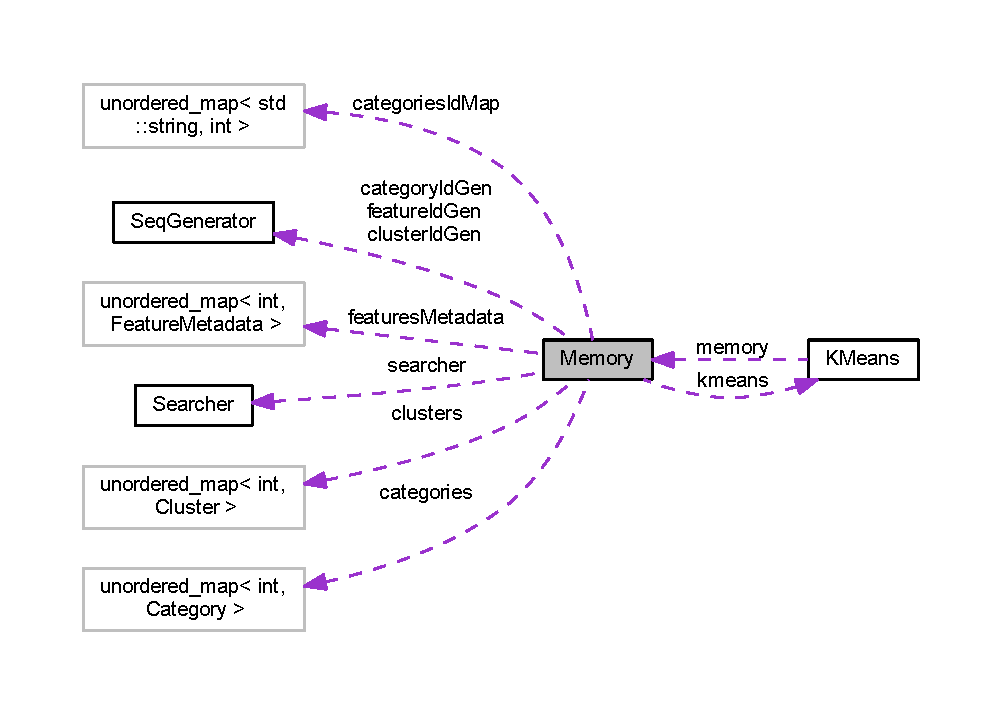
\includegraphics[width=350pt]{class_memory__coll__graph}
\end{center}
\end{figure}
\subsection*{Classes}
\begin{DoxyCompactItemize}
\item 
struct \hyperlink{struct_memory_1_1_category_view_distance}{Category\+View\+Distance}
\begin{DoxyCompactList}\small\item\em Auxiliar data structure to hold the distances between a specific object view and the categories. The distance is the euclidean distance between the respective histograms. \end{DoxyCompactList}\end{DoxyCompactItemize}
\subsection*{Public Member Functions}
\begin{DoxyCompactItemize}
\item 
\hyperlink{class_memory_a585d7bb6fc6f2237bcebf94a86b7dd99}{Memory} ()
\item 
\hyperlink{class_memory_a0ffa9759ebbf103f11132a505b93bdc0}{$\sim$\+Memory} ()
\item 
void \hyperlink{class_memory_a81ed8055b93c8e1e050d0e5f62f8a354}{update\+Centroids} (int p\+Cluster\+Id, int n\+Cluster\+Id, int feat\+Idx)
\item 
void \hyperlink{class_memory_af9c379b0907b97bc242c46bda5d58c4e}{sync\+Cluster\+Assignment} (int p\+Cluster\+Id, int n\+Cluster\+Id, int feat\+Idx)
\item 
char \hyperlink{class_memory_a02592896aaa8a91632b5c959b0a5df4c}{add\+Feature} (pcl\+::\+Histogram$<$ 153 $>$ \&feat, int \&feature\+Id)
\item 
const \hyperlink{class_feature_metadata}{Feature\+Metadata} $\ast$ \hyperlink{class_memory_ac57d713e84dce226545c1bd13007084b}{get\+Feature\+Metadata2} (const int \&key)
\item 
\hyperlink{class_feature_metadata}{Feature\+Metadata} \& \hyperlink{class_memory_a31661ea1c1d5a5fd22c0168541e82e3a}{get\+Feature\+Metadata} (const int \&key)
\item 
pcl\+::\+Histogram$<$ 153 $>$ \& \hyperlink{class_memory_abdfd86649f7e608ae6ea6af54e192fe6}{get\+Feature} (const int \&key)
\item 
void \hyperlink{class_memory_a6ba49963ea1576312687d17d8976285c}{get\+Centroids} (pcl\+::\+Point\+Cloud$<$ pcl\+::\+Histogram$<$ 153 $>$ $>$\+::Ptr \&centroids, std\+::vector$<$ int $>$ \&mapper, unordered\+\_\+map$<$ int, int $>$ \&rev\+Mapper)
\item 
void \hyperlink{class_memory_a34e8ddd680ea3a878d7564bedc8bb220}{get\+Cluster\+Points\+As\+Cloud} (Point\+Cloud$<$ Histogram$<$ 153 $>$ $>$\+::Ptr \&points, vector$<$ int $>$ \&points\+Mapper, int \&cluster\+Id)
\item 
pcl\+::\+Histogram$<$ 153 $>$ \& \hyperlink{class_memory_a56f9018e4eb1b2be429cc49b062263db}{get\+Cluster\+Centroid} (int \&cluster\+Id)
\item 
int \hyperlink{class_memory_af9c8b5c59df8b4d7ba77d08b90828d96}{get\+Cluster\+Size} (int \&cluster\+Id)
\item 
int \hyperlink{class_memory_ab71403837c0335a0e96a1e4814d4beb6}{add\+Cluster} (pcl\+::\+Histogram$<$ 153 $>$ \&centroid)
\item 
void \hyperlink{class_memory_a97043ab11f12fdd595e18ffc1fcd2291}{delete\+Cluster} (int \&cluster\+Id)
\item 
void \hyperlink{class_memory_a56ad78b70a31d0688dc160b029b8cf0e}{add\+Point\+To\+Cluster} (int \&cluster\+Id, int \&feat\+Idx)
\item 
void \hyperlink{class_memory_a3f1f42a162bbee90517642e9b2aad294}{remove\+Point\+From\+Cluster} (int \&cluster\+Id, int \&feat\+Idx)
\item 
void \hyperlink{class_memory_a638e22630bebfff55e6122b38d37c464}{un\+Assign\+All\+Points\+From\+Cluster} (int \&cluster\+Id)
\item 
void \hyperlink{class_memory_afae3d1c028779858634b0cfe0492a214}{set\+Cluster\+Centroid} (int \&cluster\+Id, int \&feat\+Idx)
\item 
void \hyperlink{class_memory_a4e5a7afc93319dd8be8f17dcfd6dc3c2}{reset\+Cluster\+Totals} (int \&cluster\+Id)
\item 
int \& \hyperlink{class_memory_aa80e09318da917906522a6cdf27b052b}{get\+Bigger\+Cluster} (int \&l\+Cluster\+Id, int \&r\+Cluster\+Id)
\item 
void \hyperlink{class_memory_a3666067f038b6765440a66cd5a3989f0}{get\+Cluster\+Points} (int \&cluster\+Id, std\+::vector$<$ int $>$ \&points\+Idx)
\item 
float \hyperlink{class_memory_aa4dae2fc7a803982c1926e2808389f73}{bss\+Betwen\+Clusters} (int \&l\+Cluster, int \&r\+Cluster)
\item 
float \hyperlink{class_memory_a74fc1ce26e175d8c992e201a3017064b}{bss} (unordered\+\_\+map$<$ int, \hyperlink{class_bss_bag}{Bss\+Bag} $>$ \&clusters\+Bss)
\item 
float \hyperlink{class_memory_a951c156d970ba7fa7a61290b1d63d95b}{wss} (std\+::vector$<$ std\+::pair$<$ int, \hyperlink{class_wss_bag}{Wss\+Bag} $>$ $>$ \&clusters\+Wss)
\item 
int \hyperlink{class_memory_a239bd8dc977f6dff458b3973e1dd4bb2}{get\+Category\+Id} (const std\+::string \&category\+Name)
\item 
int \hyperlink{class_memory_a082886bbe8c386bb7ce25a25f1b7ea8a}{add\+Category} (std\+::string category\+Name)
\item 
void \hyperlink{class_memory_a18516769c393cb146b32b42a4973176b}{add\+Point\+To\+Category} (int cat\+Id, int feat\+Idx)
\item 
void \hyperlink{class_memory_ad4a2f8d5ad6def3bca8ca8cfff122d66}{remove\+Point\+From\+Category} (int \&cat\+Id, int \&feat\+Idx)
\item 
void \hyperlink{class_memory_aeee28733d4a736e1c37a373405a532d4}{print\+Categories\+Info} ()
\item 
const std\+::string \& \hyperlink{class_memory_a80ad5f670ba87f74c170e5623f8eefc6}{get\+Category\+Name} (int category\+Id)
\item 
void \hyperlink{class_memory_a90b1dfcf945ed2b899e8c67febb23300}{assign\+View\+To\+Category} (std\+::vector$<$ int $>$ \&feats\+Idx, int category\+Id)
\item 
void \hyperlink{class_memory_af222808fa4add918c102916128ccef05}{add\+T\+P\+To\+Category} (int \&category\+Id)
\item 
void \hyperlink{class_memory_acf7decf375ad87f9997b1a295d1bf02b}{add\+F\+P\+To\+Category} (int \&category\+Id)
\item 
void \hyperlink{class_memory_a25af58af1f3c43808ec5c76f68ca6b31}{add\+F\+N\+To\+Category} (int \&category\+Id)
\item 
std\+::vector$<$ double $>$ $\ast$ \hyperlink{class_memory_a137b4cca30a6eb6bce929f53112cbb40}{get\+View\+Histogram} (std\+::vector$<$ int $>$ \&feats\+Idx, vector$<$ int $>$ \&redundancy\+Feats\+Idx)
\item 
void \hyperlink{class_memory_a9861a7a0fa823cc992f96651a08a177d}{get\+Point\+Cloud} (pcl\+::\+Point\+Cloud$<$ pcl\+::\+Histogram$<$ 153 $>$ $>$\+::Ptr \&cloud)
\item 
const int \hyperlink{class_memory_a54eea5f00668704da0dac9fb91f4773e}{get\+Cluster\+Random\+Point} (const int \&cluster)
\item 
const int \hyperlink{class_memory_a3a327af9dcb4c8f6213833b880564620}{get\+Cluster\+Random\+Point} (const int \&cluster, int \&point\+Idx)
\item 
int \hyperlink{class_memory_a7be462960a5fa5fdd8ab63dd980a56c2}{get\+View\+Category} (std\+::vector$<$ double $>$ \&view\+Histogram)
\item 
bool \hyperlink{class_memory_ae520566ff0cd3b122c0773825141f567}{is\+Redundant\+Feature} (const Histogram$<$ 153 $>$ \&search\+Feature, int feature\+Id)
\item 
void \hyperlink{class_memory_a2ead3c4cac6c9fea43047ae1c63b5a54}{remove\+Feature\+From\+Memory} (int feature\+Id)
\item 
void \hyperlink{class_memory_ab9449f7b75eeb52bf50a9e4ae08da8f0}{set\+Memory\+Decay\+Factor} (float a\+Memory\+Decay\+Factor)
\item 
float \hyperlink{class_memory_a03d6c9fa9594c8385bfe30a4c6253757}{get\+Memory\+Decay\+Factor} ()
\item 
void \hyperlink{class_memory_a035e450994077e442b5607e72b22cb0c}{set\+Memory\+Decay\+Treshold} (float a\+Memory\+Decay\+Treshold)
\item 
float \hyperlink{class_memory_ada0d9f016a8913fd6ca9c959c3a7f49a}{get\+Memory\+Decay\+Treshold} ()
\item 
long long \hyperlink{class_memory_a71384aeaf8830770030cd7e7fc8d4342}{get\+Num\+Forgotten\+Features} ()
\item 
long long \hyperlink{class_memory_aff0dd81352bffafc0989c71721f5c685}{get\+Num\+Seen\+Features} ()
\item 
long long \hyperlink{class_memory_ae5b168514b6b6bf8121526a6216a8b4e}{get\+Num\+Features\+In\+Memory} ()
\item 
long long \hyperlink{class_memory_a5ea7ba5bae1d18a31b83b7a9cc5c30cb}{get\+Num\+Redundant\+Features} ()
\item 
long long \hyperlink{class_memory_aee4eb4b1f005a36bd59a0b159d6b8a32}{get\+Num\+Seen\+Objects} ()
\item 
double \hyperlink{class_memory_aaf033cd124262162565795054e4051c9}{get\+Smallest\+Distance} ()
\item 
void \hyperlink{class_memory_a9baac2bce6c671109e3ca334c82208dd}{set\+Feature\+Redundancy\+Treshold} (double a\+Feature\+Redundancy\+Treshold)
\item 
double \hyperlink{class_memory_a6fe889030e89f7d9e473b1fc276a2def}{get\+Feature\+Redundancy\+Treshold} ()
\item 
void \hyperlink{class_memory_a87e6f6575dde85b6e823370fe8b94d16}{set\+Max\+Num\+Features\+In\+Memory} (float Max\+Num\+Features\+In\+Memory)
\item 
float \hyperlink{class_memory_ab744bd3c27190554606e4ed4ed8ce44d}{get\+Max\+Num\+Features\+In\+Memory} ()
\item 
int \hyperlink{class_memory_a9b0d2e1ab33d34fef984581921acdf7e}{get\+Num\+Forgotten\+Features\+By\+Memory\+Decay\+Factor} ()
\item 
void \hyperlink{class_memory_a797dccf9387e072227b00208545581b9}{apply\+Memory\+Decay} ()
\item 
void \hyperlink{class_memory_a743603d575e4f65c0ca1292957fd9cf2}{set\+Forget\+Features} (bool \hyperlink{class_memory_ac3c18308c5e73bd2a54fcf5cb346c638}{forget\+Features})
\item 
bool \hyperlink{class_memory_a590b5d16853c7af4c97fbffab86b9c4b}{get\+Forget\+Features} ()
\item 
void \hyperlink{class_memory_a84fcb51d7b244744161b27fe731eb1dc}{set\+Kmeans} (\hyperlink{class_k_means}{K\+Means} $\ast$a\+Kmeans)
\item 
void \hyperlink{class_memory_a6f874ffdeee770c5349c712f0b7d0952}{set\+Debug\+Mode} (bool state)
\item 
double \hyperlink{class_memory_a0317f4f9b25f51ed57b53971439b93de}{get\+Max\+Search\+Radius} ()
\item 
double \hyperlink{class_memory_a22d038e7c6a1a9c273af2f14764cdca5}{get\+Min\+Search\+Radius} ()
\item 
double \hyperlink{class_memory_a094aabdbe0f06bb5a5db61645cead64b}{get\+Max\+Wg} ()
\item 
double \hyperlink{class_memory_aba901fec044454033b0534d2a602eeb4}{get\+Min\+Wg} ()
\item 
double \hyperlink{class_memory_ada2689cdc85e2429579c0e8a75b63b8b}{get\+Max\+Wl} ()
\item 
double \hyperlink{class_memory_a8af1be617551d77f7356e2d10f796af1}{get\+Min\+Wl} ()
\item 
double \hyperlink{class_memory_af8bb8336585ad267f1ea7ca8c35b7421}{get\+Min\+Distance} ()
\item 
double \hyperlink{class_memory_a7cc17e0a04c535832ae23420901b3978}{get\+Max\+Distance} ()
\item 
void \hyperlink{class_memory_a7bd13e3f01051c375764f92c5ad25db6}{check\+Redundancy} (vector$<$ int $>$ \&feats\+Idx)
\item 
void \hyperlink{class_memory_afa0151bc0daa95b0c96aa2f5e750c7c4}{set\+G\+W\+Redist\+Search\+Radius} (double G\+Weights\+\_\+\+R\+\_\+search\+\_\+radius)
\item 
double \hyperlink{class_memory_a46da690515148bd8adaf9fbc7f42e0dc}{get\+G\+W\+Redist\+Search\+Radius} ()
\item 
int \hyperlink{class_memory_aacaf803387738204131008c1a0658fa2}{get\+N\+Clusters} ()
\item 
unordered\+\_\+map$<$ int, \hyperlink{class_cluster}{Cluster} $>$ \& \hyperlink{class_memory_ae40891f66673f8aab1f33efed7fc9750}{get\+Clusters} ()
\item 
unordered\+\_\+map$<$ int, \hyperlink{class_category}{Category} $>$ \& \hyperlink{class_memory_a51f0f9c3a202dd21c9dbae0dbeadaf68}{get\+Categories} ()
\item 
int \hyperlink{class_memory_a02757aec9ff7f8285a28213e9777d56a}{generate\+Cluster\+Id} ()
\item 
int \hyperlink{class_memory_ab31cf2fb776b10af99265c55ef1703d2}{generate\+Category\+Id} ()
\item 
int \hyperlink{class_memory_aa39a1f59ecca722d41b77e34f7c5763c}{generate\+Feature\+Id} ()
\item 
int \hyperlink{class_memory_a91ac81338123d3b57a7f5ee62db8ec8d}{size} () const
\item 
unordered\+\_\+map$<$ int, \hyperlink{class_feature_metadata}{Feature\+Metadata} $>$ \& \hyperlink{class_memory_a0b1d14bfe43af3d3a0353dea8c6eca35}{get\+Features} ()
\end{DoxyCompactItemize}
\subsection*{Protected Member Functions}
\begin{DoxyCompactItemize}
\item 
void \hyperlink{class_memory_aa98d92e8d824eeb2e5699d6e1e2ff44b}{forget\+Redundant\+Features} (const vector$<$ int $>$ features\+Ids)
\item 
void \hyperlink{class_memory_ae4c5bcd99c34f0bcc62e0fcc8bac57fc}{rem\+Feature\+From\+Memory} (int feature\+Id, \hyperlink{class_feature_metadata}{Feature\+Metadata} \&feature\+Metadata)
\item 
void \hyperlink{class_memory_a1f36348fab81a50b9bbe16986b7a0337}{redistribute\+Local\+Weights} (unordered\+\_\+set$<$ int $>$ \&to\+Forget, int category\+Id)
\item 
void \hyperlink{class_memory_a53d9e1a15f774f05c68eeb1ab1042cb8}{redistribute\+Local\+Weights} (int feature\+Id, \hyperlink{class_feature_metadata}{Feature\+Metadata} \&feature\+Metadata)
\item 
void \hyperlink{class_memory_a0dbad1e7f9ae70aaf65dd733f3e6c9b9}{remove\+Point\+From\+Cluster2} (int cluster\+Id, int feat\+Idx)
\item 
double \hyperlink{class_memory_af45cd527f0c6fad40154e19b42d8fce3}{get\+Search\+Radius} (int feature\+Id, \hyperlink{class_feature_metadata}{Feature\+Metadata} \&feature\+Metadata, int k)
\item 
void \hyperlink{class_memory_ac99702a46e98175ec1b05dfd6001eaab}{remove\+Point\+From\+Category2} (int category\+Id, int feat\+Idx)
\item 
void \hyperlink{class_memory_a8b6338bb727061f8c55e0e5df04204d4}{redistribute\+Global\+Weights} (int feature\+Id, \hyperlink{class_feature_metadata}{Feature\+Metadata} \&feature\+Metadata, double search\+Radius)
\item 
void \hyperlink{class_memory_a3b697274988fa315d03015d854e3f813}{redistribute\+Global\+Weights} (unordered\+\_\+set$<$ int $>$ \&to\+Forget, Kd\+Tree\+F\+L\+A\+NN$<$ Histogram$<$ 153 $>$ $>$ \&kdtree, vector$<$ int $>$ \&mapping, double search\+Radius)
\item 
float \hyperlink{class_memory_ac31686018cb26f05d51714e057af954b}{apply\+Memory\+Decay\+Factor} (float weight)
\item 
void \hyperlink{class_memory_add3f52953d79c8ace1de5d7c667a33d1}{forget\+Feature} (int feature\+Id)
\end{DoxyCompactItemize}
\subsection*{Protected Attributes}
\begin{DoxyCompactItemize}
\item 
double \hyperlink{class_memory_a26d5cb9d95759ae04db5e3c89dbae345}{max\+Search\+Radius}
\item 
double \hyperlink{class_memory_a80399a94aa2cb5d06d4e7b4b578b73b8}{min\+Search\+Radius}
\item 
double \hyperlink{class_memory_a657eb626fc7fa089dea3274b87658d81}{max\+Wg}
\item 
double \hyperlink{class_memory_a1bf6db077ded1e0f826a09b89b543695}{min\+Wg}
\item 
double \hyperlink{class_memory_af3eb8d644c9b8bef76a262234ae6c070}{max\+Wl}
\item 
double \hyperlink{class_memory_a9172ef7604d582af5b7d38ecd5245e47}{min\+Wl}
\item 
double \hyperlink{class_memory_ac3ffdf66cf9b1144dad6aa9f39040db6}{min\+Distance}
\item 
double \hyperlink{class_memory_aed07b3dddef97de3f7eaca420ff00df3}{max\+Distance}
\item 
double \hyperlink{class_memory_a65e77a8517b78627da8bc33dd5f7925b}{fixed\+Search\+Radius}
\item 
bool \hyperlink{class_memory_a8607f19b7d9871eeb12ca94d7938c710}{D\+E\+B\+UG}
\item 
\hyperlink{class_k_means}{K\+Means} $\ast$ \hyperlink{class_memory_a4d1844ac4c1ff005f5a87373783a96f1}{kmeans}
\item 
double \hyperlink{class_memory_a4b73ac8b78b6a1003e946f61697fe65d}{smallest\+Distance}
\item 
\hyperlink{class_searcher}{Searcher} \hyperlink{class_memory_a28d1cf97ef560d4f096a506ef53a1410}{searcher}
\item 
double \hyperlink{class_memory_a5b4e6c308dedb36e66bef5b85f5a1d1a}{feature\+Redundancy\+Treshold}
\item 
float \hyperlink{class_memory_ad82103f1fc27ceab9c6e20c8c96ddfb2}{memory\+Decay\+Factor}
\item 
float \hyperlink{class_memory_a5cbea14d34dceeca8d8f3fd82674a7f0}{memory\+Decay\+Treshold}
\item 
int \hyperlink{class_memory_aa351103686a0f8230ca638fbf0b2dc5b}{n\+Forgotten\+Features\+By\+Memory\+Decay\+Factor}
\item 
bool \hyperlink{class_memory_ac3c18308c5e73bd2a54fcf5cb346c638}{forget\+Features}
\item 
long long \hyperlink{class_memory_a35ac41aee3f23446e2f34e492818007e}{num\+Features\+In\+Memory}
\item 
long long \hyperlink{class_memory_ae10824d7cf347234fd910fa3a4e6a9c7}{num\+Seen\+Features}
\item 
long long \hyperlink{class_memory_a3b7f28c5be1d201bb41cdbc90646fb4b}{num\+Seen\+Objects}
\item 
long long \hyperlink{class_memory_ae3c078fe2fb8bc942d13ede6a2eb951b}{num\+Redundant\+Features}
\item 
long long \hyperlink{class_memory_a01e573fd360050d1d87e4702eeec77ff}{num\+Forgotten\+Features}
\item 
long long \hyperlink{class_memory_a39621632b0a7c038b589cdb1c7402c02}{max\+Num\+Features\+In\+Memory}
\item 
unordered\+\_\+map$<$ int, \hyperlink{class_feature_metadata}{Feature\+Metadata} $>$ \hyperlink{class_memory_a70a3ffe94ecd25fa10c683b3fac6328b}{features\+Metadata}
\item 
unordered\+\_\+map$<$ int, \hyperlink{class_cluster}{Cluster} $>$ \hyperlink{class_memory_a9836b99d2ec4b06e98a90aa31d16439a}{clusters}
\item 
vector$<$ int $>$ \hyperlink{class_memory_a9bb05f7f61a8eb13c91fa9f99d1962a6}{new\+Seen\+Features\+Ids}
\item 
\hyperlink{class_seq_generator}{Seq\+Generator} \hyperlink{class_memory_aedc30fc567e03bfa3fa43fb47ba506f8}{cluster\+Id\+Gen}
\item 
unordered\+\_\+map$<$ int, \hyperlink{class_category}{Category} $>$ \hyperlink{class_memory_ab7733936ac814bc1f834a79fd868c8d9}{categories}
\item 
unordered\+\_\+map$<$ std\+::string, int $>$ \hyperlink{class_memory_aa40e026a0318c101754d065725a7b72d}{categories\+Id\+Map}
\item 
\hyperlink{class_seq_generator}{Seq\+Generator} \hyperlink{class_memory_a9e1a47adebdbbbade810a92215903ce1}{category\+Id\+Gen}
\item 
\hyperlink{class_seq_generator}{Seq\+Generator} \hyperlink{class_memory_a3c07af17879875325b9073fc77f56e3f}{feature\+Id\+Gen}
\end{DoxyCompactItemize}


\subsection{Detailed Description}
Main structure of the application. Holds the applications\textquotesingle{} memory. 

Definition at line 30 of file Memory.\+h.



\subsection{Constructor \& Destructor Documentation}
\mbox{\Hypertarget{class_memory_a585d7bb6fc6f2237bcebf94a86b7dd99}\label{class_memory_a585d7bb6fc6f2237bcebf94a86b7dd99}} 
\index{Memory@{Memory}!Memory@{Memory}}
\index{Memory@{Memory}!Memory@{Memory}}
\subsubsection{\texorpdfstring{Memory()}{Memory()}}
{\footnotesize\ttfamily Memory\+::\+Memory (\begin{DoxyParamCaption}{ }\end{DoxyParamCaption})}



Definition at line 34 of file Memory.\+cpp.

\mbox{\Hypertarget{class_memory_a0ffa9759ebbf103f11132a505b93bdc0}\label{class_memory_a0ffa9759ebbf103f11132a505b93bdc0}} 
\index{Memory@{Memory}!````~Memory@{$\sim$\+Memory}}
\index{````~Memory@{$\sim$\+Memory}!Memory@{Memory}}
\subsubsection{\texorpdfstring{$\sim$\+Memory()}{~Memory()}}
{\footnotesize\ttfamily Memory\+::$\sim$\+Memory (\begin{DoxyParamCaption}{ }\end{DoxyParamCaption})}



Definition at line 78 of file Memory.\+cpp.



\subsection{Member Function Documentation}
\mbox{\Hypertarget{class_memory_a082886bbe8c386bb7ce25a25f1b7ea8a}\label{class_memory_a082886bbe8c386bb7ce25a25f1b7ea8a}} 
\index{Memory@{Memory}!add\+Category@{add\+Category}}
\index{add\+Category@{add\+Category}!Memory@{Memory}}
\subsubsection{\texorpdfstring{add\+Category()}{addCategory()}}
{\footnotesize\ttfamily int Memory\+::add\+Category (\begin{DoxyParamCaption}\item[{std\+::string}]{category\+Name }\end{DoxyParamCaption})}

Create a new category


\begin{DoxyParams}[1]{Parameters}
\mbox{\tt in}  & {\em name} & the name of the category\\
\hline
\end{DoxyParams}
Returns the identifier of the created category 

Definition at line 814 of file Memory.\+cpp.

\mbox{\Hypertarget{class_memory_ab71403837c0335a0e96a1e4814d4beb6}\label{class_memory_ab71403837c0335a0e96a1e4814d4beb6}} 
\index{Memory@{Memory}!add\+Cluster@{add\+Cluster}}
\index{add\+Cluster@{add\+Cluster}!Memory@{Memory}}
\subsubsection{\texorpdfstring{add\+Cluster()}{addCluster()}}
{\footnotesize\ttfamily int Memory\+::add\+Cluster (\begin{DoxyParamCaption}\item[{pcl\+::\+Histogram$<$ 153 $>$ \&}]{centroid }\end{DoxyParamCaption})}

Create a new cluster


\begin{DoxyParams}[1]{Parameters}
\mbox{\tt in}  & {\em centroid} & the centroid of the cluster\\
\hline
\end{DoxyParams}
Returns the identifier of the created cluster 

Definition at line 560 of file Memory.\+cpp.

\mbox{\Hypertarget{class_memory_a02592896aaa8a91632b5c959b0a5df4c}\label{class_memory_a02592896aaa8a91632b5c959b0a5df4c}} 
\index{Memory@{Memory}!add\+Feature@{add\+Feature}}
\index{add\+Feature@{add\+Feature}!Memory@{Memory}}
\subsubsection{\texorpdfstring{add\+Feature()}{addFeature()}}
{\footnotesize\ttfamily char Memory\+::add\+Feature (\begin{DoxyParamCaption}\item[{pcl\+::\+Histogram$<$ 153 $>$ \&}]{feat,  }\item[{int \&}]{feature\+Id }\end{DoxyParamCaption})}

Adds a feature (point) to memory-\/ It also adds the corresponding metadata to the feature metadata structure.


\begin{DoxyParams}[1]{Parameters}
\mbox{\tt in}  & {\em feat} & the feature to be added to the memory\\
\hline
\end{DoxyParams}
Returns the identifier of the created feature. 

Definition at line 120 of file Memory.\+cpp.

\mbox{\Hypertarget{class_memory_a25af58af1f3c43808ec5c76f68ca6b31}\label{class_memory_a25af58af1f3c43808ec5c76f68ca6b31}} 
\index{Memory@{Memory}!add\+F\+N\+To\+Category@{add\+F\+N\+To\+Category}}
\index{add\+F\+N\+To\+Category@{add\+F\+N\+To\+Category}!Memory@{Memory}}
\subsubsection{\texorpdfstring{add\+F\+N\+To\+Category()}{addFNToCategory()}}
{\footnotesize\ttfamily void Memory\+::add\+F\+N\+To\+Category (\begin{DoxyParamCaption}\item[{int \&}]{category\+Id }\end{DoxyParamCaption})}

Increments the False Negatives count for the specified category


\begin{DoxyParams}[1]{Parameters}
\mbox{\tt in}  & {\em category\+Id} & the category identifier \\
\hline
\end{DoxyParams}


Definition at line 914 of file Memory.\+cpp.

\mbox{\Hypertarget{class_memory_acf7decf375ad87f9997b1a295d1bf02b}\label{class_memory_acf7decf375ad87f9997b1a295d1bf02b}} 
\index{Memory@{Memory}!add\+F\+P\+To\+Category@{add\+F\+P\+To\+Category}}
\index{add\+F\+P\+To\+Category@{add\+F\+P\+To\+Category}!Memory@{Memory}}
\subsubsection{\texorpdfstring{add\+F\+P\+To\+Category()}{addFPToCategory()}}
{\footnotesize\ttfamily void Memory\+::add\+F\+P\+To\+Category (\begin{DoxyParamCaption}\item[{int \&}]{category\+Id }\end{DoxyParamCaption})}

Increments the False Positives count for the specified category


\begin{DoxyParams}[1]{Parameters}
\mbox{\tt in}  & {\em category\+Id} & the category identifier \\
\hline
\end{DoxyParams}


Definition at line 910 of file Memory.\+cpp.

\mbox{\Hypertarget{class_memory_a18516769c393cb146b32b42a4973176b}\label{class_memory_a18516769c393cb146b32b42a4973176b}} 
\index{Memory@{Memory}!add\+Point\+To\+Category@{add\+Point\+To\+Category}}
\index{add\+Point\+To\+Category@{add\+Point\+To\+Category}!Memory@{Memory}}
\subsubsection{\texorpdfstring{add\+Point\+To\+Category()}{addPointToCategory()}}
{\footnotesize\ttfamily void Memory\+::add\+Point\+To\+Category (\begin{DoxyParamCaption}\item[{int}]{cat\+Id,  }\item[{int}]{feat\+Idx }\end{DoxyParamCaption})}

Add a feature to the category


\begin{DoxyParams}[1]{Parameters}
\mbox{\tt in}  & {\em cat\+Id} & the identifier of the category \\
\hline
\mbox{\tt in}  & {\em feat\+Idx} & the index of the feature (in main memory) to add to the category \\
\hline
\end{DoxyParams}


Definition at line 834 of file Memory.\+cpp.

\mbox{\Hypertarget{class_memory_a56ad78b70a31d0688dc160b029b8cf0e}\label{class_memory_a56ad78b70a31d0688dc160b029b8cf0e}} 
\index{Memory@{Memory}!add\+Point\+To\+Cluster@{add\+Point\+To\+Cluster}}
\index{add\+Point\+To\+Cluster@{add\+Point\+To\+Cluster}!Memory@{Memory}}
\subsubsection{\texorpdfstring{add\+Point\+To\+Cluster()}{addPointToCluster()}}
{\footnotesize\ttfamily void Memory\+::add\+Point\+To\+Cluster (\begin{DoxyParamCaption}\item[{int \&}]{cluster\+Id,  }\item[{int \&}]{feat\+Idx }\end{DoxyParamCaption})}

Add a feature to the cluster


\begin{DoxyParams}[1]{Parameters}
\mbox{\tt in}  & {\em cluster\+Id} & the identifier of the cluster \\
\hline
\mbox{\tt in}  & {\em feat\+Idx} & the index of the feature (in main memory) to add to the cluster \\
\hline
\end{DoxyParams}


Definition at line 572 of file Memory.\+cpp.

\mbox{\Hypertarget{class_memory_af222808fa4add918c102916128ccef05}\label{class_memory_af222808fa4add918c102916128ccef05}} 
\index{Memory@{Memory}!add\+T\+P\+To\+Category@{add\+T\+P\+To\+Category}}
\index{add\+T\+P\+To\+Category@{add\+T\+P\+To\+Category}!Memory@{Memory}}
\subsubsection{\texorpdfstring{add\+T\+P\+To\+Category()}{addTPToCategory()}}
{\footnotesize\ttfamily void Memory\+::add\+T\+P\+To\+Category (\begin{DoxyParamCaption}\item[{int \&}]{category\+Id }\end{DoxyParamCaption})}

Increments the True Positives count for the specified category


\begin{DoxyParams}[1]{Parameters}
\mbox{\tt in}  & {\em category\+Id} & the category identifier \\
\hline
\end{DoxyParams}


Definition at line 906 of file Memory.\+cpp.

\mbox{\Hypertarget{class_memory_a797dccf9387e072227b00208545581b9}\label{class_memory_a797dccf9387e072227b00208545581b9}} 
\index{Memory@{Memory}!apply\+Memory\+Decay@{apply\+Memory\+Decay}}
\index{apply\+Memory\+Decay@{apply\+Memory\+Decay}!Memory@{Memory}}
\subsubsection{\texorpdfstring{apply\+Memory\+Decay()}{applyMemoryDecay()}}
{\footnotesize\ttfamily void Memory\+::apply\+Memory\+Decay (\begin{DoxyParamCaption}{ }\end{DoxyParamCaption})}

Applies the memory decay factor to all features in memory. Call this function before adding new features or all features will be affected by the decay factor including the new added ones. Maybe it makes no sense to apply the memory decay factor to fresh new seen features! The memory decay factor is applied to the local and global weights\+: the category and clusters weights of a feature, respectively.

If after applying the decay memory factor the global weight of a feature drops bellow a given treshold, that feature will be forgotten.

Open issues\+:
\begin{DoxyItemize}
\item The best value for the \hyperlink{class_memory}{Memory} Decay Threshold has to be determined more precisely and accurately!
\end{DoxyItemize}

This should be the main method used to forget features and to control the number of features in memory.
\begin{DoxyItemize}
\item This does not, of course, include redundancy! 
\end{DoxyItemize}

Definition at line 945 of file Memory.\+cpp.

\mbox{\Hypertarget{class_memory_ac31686018cb26f05d51714e057af954b}\label{class_memory_ac31686018cb26f05d51714e057af954b}} 
\index{Memory@{Memory}!apply\+Memory\+Decay\+Factor@{apply\+Memory\+Decay\+Factor}}
\index{apply\+Memory\+Decay\+Factor@{apply\+Memory\+Decay\+Factor}!Memory@{Memory}}
\subsubsection{\texorpdfstring{apply\+Memory\+Decay\+Factor()}{applyMemoryDecayFactor()}}
{\footnotesize\ttfamily float Memory\+::apply\+Memory\+Decay\+Factor (\begin{DoxyParamCaption}\item[{float}]{weight }\end{DoxyParamCaption})\hspace{0.3cm}{\ttfamily [inline]}, {\ttfamily [protected]}}

Applies the memory decay factor to a given weight. The formula follows\+: given weight $\ast$= memory\+Decay\+Factor 

Definition at line 676 of file Memory.\+h.

\mbox{\Hypertarget{class_memory_a90b1dfcf945ed2b899e8c67febb23300}\label{class_memory_a90b1dfcf945ed2b899e8c67febb23300}} 
\index{Memory@{Memory}!assign\+View\+To\+Category@{assign\+View\+To\+Category}}
\index{assign\+View\+To\+Category@{assign\+View\+To\+Category}!Memory@{Memory}}
\subsubsection{\texorpdfstring{assign\+View\+To\+Category()}{assignViewToCategory()}}
{\footnotesize\ttfamily void Memory\+::assign\+View\+To\+Category (\begin{DoxyParamCaption}\item[{std\+::vector$<$ int $>$ \&}]{feats\+Idx,  }\item[{int}]{category\+Id }\end{DoxyParamCaption})}

Assings the specified features ids to the specified category. . $\ast$ 
\begin{DoxyParams}[1]{Parameters}
\mbox{\tt in}  & {\em feats\+Idx} & features ids to assign \\
\hline
\mbox{\tt in}  & {\em category\+Id} & the identifier of the category to assign the features to \\
\hline
\end{DoxyParams}


Definition at line 852 of file Memory.\+cpp.

\mbox{\Hypertarget{class_memory_a74fc1ce26e175d8c992e201a3017064b}\label{class_memory_a74fc1ce26e175d8c992e201a3017064b}} 
\index{Memory@{Memory}!bss@{bss}}
\index{bss@{bss}!Memory@{Memory}}
\subsubsection{\texorpdfstring{bss()}{bss()}}
{\footnotesize\ttfamily float Memory\+::bss (\begin{DoxyParamCaption}\item[{unordered\+\_\+map$<$ int, \hyperlink{class_bss_bag}{Bss\+Bag} $>$ \&}]{clusters\+Bss }\end{DoxyParamCaption})}

Compute B\+SS (Between cluster Sum of Squares) measure


\begin{DoxyParams}[1]{Parameters}
\mbox{\tt out}  & {\em clusters\+Bss} & vector holding the \textquotesingle{}partial bss\textquotesingle{} computed for every cluster\\
\hline
\end{DoxyParams}
Returns the total bss 

Definition at line 650 of file Memory.\+cpp.

\mbox{\Hypertarget{class_memory_aa4dae2fc7a803982c1926e2808389f73}\label{class_memory_aa4dae2fc7a803982c1926e2808389f73}} 
\index{Memory@{Memory}!bss\+Betwen\+Clusters@{bss\+Betwen\+Clusters}}
\index{bss\+Betwen\+Clusters@{bss\+Betwen\+Clusters}!Memory@{Memory}}
\subsubsection{\texorpdfstring{bss\+Betwen\+Clusters()}{bssBetwenClusters()}}
{\footnotesize\ttfamily float Memory\+::bss\+Betwen\+Clusters (\begin{DoxyParamCaption}\item[{int \&}]{l\+Cluster,  }\item[{int \&}]{r\+Cluster }\end{DoxyParamCaption})}

Compute the distance between two clusters


\begin{DoxyParams}[1]{Parameters}
\mbox{\tt in}  & {\em l\+Cluster} & the identifier of the first cluster \\
\hline
\mbox{\tt in}  & {\em r\+Cluster} & the identifier of the second cluster \\
\hline
\end{DoxyParams}


Definition at line 633 of file Memory.\+cpp.

\mbox{\Hypertarget{class_memory_a7bd13e3f01051c375764f92c5ad25db6}\label{class_memory_a7bd13e3f01051c375764f92c5ad25db6}} 
\index{Memory@{Memory}!check\+Redundancy@{check\+Redundancy}}
\index{check\+Redundancy@{check\+Redundancy}!Memory@{Memory}}
\subsubsection{\texorpdfstring{check\+Redundancy()}{checkRedundancy()}}
{\footnotesize\ttfamily void Memory\+::check\+Redundancy (\begin{DoxyParamCaption}\item[{vector$<$ int $>$ \&}]{feats\+Idx }\end{DoxyParamCaption})}

Checks redundancy for every feature id specified in the feats\+Idx vector. These features are assumed to be new seen features. This function is currently using snapshots to check redundancy and to redistribute weights.


\begin{DoxyParams}[1]{Parameters}
\mbox{\tt in}  & {\em feats\+Idx} & the id of the features to check for redundancy. \\
\hline
\end{DoxyParams}


Definition at line 137 of file Memory.\+cpp.

\mbox{\Hypertarget{class_memory_a97043ab11f12fdd595e18ffc1fcd2291}\label{class_memory_a97043ab11f12fdd595e18ffc1fcd2291}} 
\index{Memory@{Memory}!delete\+Cluster@{delete\+Cluster}}
\index{delete\+Cluster@{delete\+Cluster}!Memory@{Memory}}
\subsubsection{\texorpdfstring{delete\+Cluster()}{deleteCluster()}}
{\footnotesize\ttfamily void Memory\+::delete\+Cluster (\begin{DoxyParamCaption}\item[{int \&}]{cluster\+Id }\end{DoxyParamCaption})}

Delete a cluster


\begin{DoxyParams}[1]{Parameters}
\mbox{\tt in}  & {\em cluster\+Id} & the identifier of the cluster to delete \\
\hline
\end{DoxyParams}


Definition at line 568 of file Memory.\+cpp.

\mbox{\Hypertarget{class_memory_add3f52953d79c8ace1de5d7c667a33d1}\label{class_memory_add3f52953d79c8ace1de5d7c667a33d1}} 
\index{Memory@{Memory}!forget\+Feature@{forget\+Feature}}
\index{forget\+Feature@{forget\+Feature}!Memory@{Memory}}
\subsubsection{\texorpdfstring{forget\+Feature()}{forgetFeature()}}
{\footnotesize\ttfamily void Memory\+::forget\+Feature (\begin{DoxyParamCaption}\item[{int}]{feature\+Id }\end{DoxyParamCaption})\hspace{0.3cm}{\ttfamily [protected]}}

Forgets a given feature i.\+e., 1 -\/ redistribute global weights 2 -\/ redistribute local weights 3 -\/ update the cluster centroid to wich the feature is assign 4 -\/ remove the feature from memory 5 -\/ reorganize the clusters if needed 

Definition at line 1379 of file Memory.\+cpp.

\mbox{\Hypertarget{class_memory_aa98d92e8d824eeb2e5699d6e1e2ff44b}\label{class_memory_aa98d92e8d824eeb2e5699d6e1e2ff44b}} 
\index{Memory@{Memory}!forget\+Redundant\+Features@{forget\+Redundant\+Features}}
\index{forget\+Redundant\+Features@{forget\+Redundant\+Features}!Memory@{Memory}}
\subsubsection{\texorpdfstring{forget\+Redundant\+Features()}{forgetRedundantFeatures()}}
{\footnotesize\ttfamily void Memory\+::forget\+Redundant\+Features (\begin{DoxyParamCaption}\item[{const vector$<$ int $>$}]{features\+Ids }\end{DoxyParamCaption})\hspace{0.3cm}{\ttfamily [protected]}}

Checks if a feature is redundant. Don\textquotesingle{}t use this function. I think, I\textquotesingle{}m almost sure, it is not checking redundancy by itself and mutual redundancy properly. 

Definition at line 1598 of file Memory.\+cpp.

\mbox{\Hypertarget{class_memory_ab31cf2fb776b10af99265c55ef1703d2}\label{class_memory_ab31cf2fb776b10af99265c55ef1703d2}} 
\index{Memory@{Memory}!generate\+Category\+Id@{generate\+Category\+Id}}
\index{generate\+Category\+Id@{generate\+Category\+Id}!Memory@{Memory}}
\subsubsection{\texorpdfstring{generate\+Category\+Id()}{generateCategoryId()}}
{\footnotesize\ttfamily int Memory\+::generate\+Category\+Id (\begin{DoxyParamCaption}{ }\end{DoxyParamCaption})\hspace{0.3cm}{\ttfamily [inline]}}

Get a unique integer identifier for the category (map key). 

Definition at line 796 of file Memory.\+h.

\mbox{\Hypertarget{class_memory_a02757aec9ff7f8285a28213e9777d56a}\label{class_memory_a02757aec9ff7f8285a28213e9777d56a}} 
\index{Memory@{Memory}!generate\+Cluster\+Id@{generate\+Cluster\+Id}}
\index{generate\+Cluster\+Id@{generate\+Cluster\+Id}!Memory@{Memory}}
\subsubsection{\texorpdfstring{generate\+Cluster\+Id()}{generateClusterId()}}
{\footnotesize\ttfamily int Memory\+::generate\+Cluster\+Id (\begin{DoxyParamCaption}{ }\end{DoxyParamCaption})\hspace{0.3cm}{\ttfamily [inline]}}

Get a unique integer identifier for the cluster (map key). 

Definition at line 789 of file Memory.\+h.

\mbox{\Hypertarget{class_memory_aa39a1f59ecca722d41b77e34f7c5763c}\label{class_memory_aa39a1f59ecca722d41b77e34f7c5763c}} 
\index{Memory@{Memory}!generate\+Feature\+Id@{generate\+Feature\+Id}}
\index{generate\+Feature\+Id@{generate\+Feature\+Id}!Memory@{Memory}}
\subsubsection{\texorpdfstring{generate\+Feature\+Id()}{generateFeatureId()}}
{\footnotesize\ttfamily int Memory\+::generate\+Feature\+Id (\begin{DoxyParamCaption}{ }\end{DoxyParamCaption})\hspace{0.3cm}{\ttfamily [inline]}}

Get a unique integer identifier for the feature (map key). 

Definition at line 803 of file Memory.\+h.

\mbox{\Hypertarget{class_memory_aa80e09318da917906522a6cdf27b052b}\label{class_memory_aa80e09318da917906522a6cdf27b052b}} 
\index{Memory@{Memory}!get\+Bigger\+Cluster@{get\+Bigger\+Cluster}}
\index{get\+Bigger\+Cluster@{get\+Bigger\+Cluster}!Memory@{Memory}}
\subsubsection{\texorpdfstring{get\+Bigger\+Cluster()}{getBiggerCluster()}}
{\footnotesize\ttfamily int \& Memory\+::get\+Bigger\+Cluster (\begin{DoxyParamCaption}\item[{int \&}]{l\+Cluster\+Id,  }\item[{int \&}]{r\+Cluster\+Id }\end{DoxyParamCaption})}

Returns the cluster identifier for the biggest cluster of the 2 clusters specified


\begin{DoxyParams}[1]{Parameters}
\mbox{\tt in}  & {\em l\+Cluster\+Id} & the identifier of the first cluster to be compared in terms of size \\
\hline
\mbox{\tt in}  & {\em r\+Cluster\+Id} & the identifier of the second cluster to be compared in terms of size \\
\hline
\end{DoxyParams}


Definition at line 620 of file Memory.\+cpp.

\mbox{\Hypertarget{class_memory_a51f0f9c3a202dd21c9dbae0dbeadaf68}\label{class_memory_a51f0f9c3a202dd21c9dbae0dbeadaf68}} 
\index{Memory@{Memory}!get\+Categories@{get\+Categories}}
\index{get\+Categories@{get\+Categories}!Memory@{Memory}}
\subsubsection{\texorpdfstring{get\+Categories()}{getCategories()}}
{\footnotesize\ttfamily unordered\+\_\+map$<$int, \hyperlink{class_category}{Category}$>$\& Memory\+::get\+Categories (\begin{DoxyParamCaption}{ }\end{DoxyParamCaption})\hspace{0.3cm}{\ttfamily [inline]}}



Definition at line 782 of file Memory.\+h.

\mbox{\Hypertarget{class_memory_a239bd8dc977f6dff458b3973e1dd4bb2}\label{class_memory_a239bd8dc977f6dff458b3973e1dd4bb2}} 
\index{Memory@{Memory}!get\+Category\+Id@{get\+Category\+Id}}
\index{get\+Category\+Id@{get\+Category\+Id}!Memory@{Memory}}
\subsubsection{\texorpdfstring{get\+Category\+Id()}{getCategoryId()}}
{\footnotesize\ttfamily int Memory\+::get\+Category\+Id (\begin{DoxyParamCaption}\item[{const std\+::string \&}]{category\+Name }\end{DoxyParamCaption})}

Return category identifier for specified categoy name


\begin{DoxyParams}[1]{Parameters}
\mbox{\tt in}  & {\em cat} & the category name to return the identifier \\
\hline
\end{DoxyParams}


Definition at line 802 of file Memory.\+cpp.

\mbox{\Hypertarget{class_memory_a80ad5f670ba87f74c170e5623f8eefc6}\label{class_memory_a80ad5f670ba87f74c170e5623f8eefc6}} 
\index{Memory@{Memory}!get\+Category\+Name@{get\+Category\+Name}}
\index{get\+Category\+Name@{get\+Category\+Name}!Memory@{Memory}}
\subsubsection{\texorpdfstring{get\+Category\+Name()}{getCategoryName()}}
{\footnotesize\ttfamily const std\+::string \& Memory\+::get\+Category\+Name (\begin{DoxyParamCaption}\item[{int}]{category\+Id }\end{DoxyParamCaption})}



Definition at line 777 of file Memory.\+cpp.

\mbox{\Hypertarget{class_memory_a6ba49963ea1576312687d17d8976285c}\label{class_memory_a6ba49963ea1576312687d17d8976285c}} 
\index{Memory@{Memory}!get\+Centroids@{get\+Centroids}}
\index{get\+Centroids@{get\+Centroids}!Memory@{Memory}}
\subsubsection{\texorpdfstring{get\+Centroids()}{getCentroids()}}
{\footnotesize\ttfamily void Memory\+::get\+Centroids (\begin{DoxyParamCaption}\item[{pcl\+::\+Point\+Cloud$<$ pcl\+::\+Histogram$<$ 153 $>$ $>$\+::Ptr \&}]{centroids,  }\item[{std\+::vector$<$ int $>$ \&}]{mapper,  }\item[{unordered\+\_\+map$<$ int, int $>$ \&}]{rev\+Mapper }\end{DoxyParamCaption})}

Retrieve the cluster centroids stored in memory.


\begin{DoxyParams}[1]{Parameters}
\mbox{\tt out}  & {\em centroids} & the centroids of the clusters \\
\hline
\mbox{\tt out}  & {\em mapper} & a structure that maps from the centroids vector indexes to the cluster identifiers \\
\hline
\mbox{\tt out}  & {\em rev\+Mapper} & a structure that maps from the cluster identifiers to the centroids vector indexes \\
\hline
\end{DoxyParams}


Definition at line 518 of file Memory.\+cpp.

\mbox{\Hypertarget{class_memory_a56f9018e4eb1b2be429cc49b062263db}\label{class_memory_a56f9018e4eb1b2be429cc49b062263db}} 
\index{Memory@{Memory}!get\+Cluster\+Centroid@{get\+Cluster\+Centroid}}
\index{get\+Cluster\+Centroid@{get\+Cluster\+Centroid}!Memory@{Memory}}
\subsubsection{\texorpdfstring{get\+Cluster\+Centroid()}{getClusterCentroid()}}
{\footnotesize\ttfamily Histogram$<$ 153 $>$ \& Memory\+::get\+Cluster\+Centroid (\begin{DoxyParamCaption}\item[{int \&}]{cluster\+Id }\end{DoxyParamCaption})}

Get the centroid of a specific cluster


\begin{DoxyParams}[1]{Parameters}
\mbox{\tt in}  & {\em cluster\+Id} & the cluster identifier \\
\hline
\end{DoxyParams}


Definition at line 556 of file Memory.\+cpp.

\mbox{\Hypertarget{class_memory_a3666067f038b6765440a66cd5a3989f0}\label{class_memory_a3666067f038b6765440a66cd5a3989f0}} 
\index{Memory@{Memory}!get\+Cluster\+Points@{get\+Cluster\+Points}}
\index{get\+Cluster\+Points@{get\+Cluster\+Points}!Memory@{Memory}}
\subsubsection{\texorpdfstring{get\+Cluster\+Points()}{getClusterPoints()}}
{\footnotesize\ttfamily void Memory\+::get\+Cluster\+Points (\begin{DoxyParamCaption}\item[{int \&}]{cluster\+Id,  }\item[{std\+::vector$<$ int $>$ \&}]{points\+Idx }\end{DoxyParamCaption})}

Return the list of features assigned to the specified cluster


\begin{DoxyParams}[1]{Parameters}
\mbox{\tt in}  & {\em cluster\+Id} & the identifier of the cluster to get the list of assigned features \\
\hline
\mbox{\tt out}  & {\em points\+Idx} & the list of features \\
\hline
\end{DoxyParams}


Definition at line 625 of file Memory.\+cpp.

\mbox{\Hypertarget{class_memory_a34e8ddd680ea3a878d7564bedc8bb220}\label{class_memory_a34e8ddd680ea3a878d7564bedc8bb220}} 
\index{Memory@{Memory}!get\+Cluster\+Points\+As\+Cloud@{get\+Cluster\+Points\+As\+Cloud}}
\index{get\+Cluster\+Points\+As\+Cloud@{get\+Cluster\+Points\+As\+Cloud}!Memory@{Memory}}
\subsubsection{\texorpdfstring{get\+Cluster\+Points\+As\+Cloud()}{getClusterPointsAsCloud()}}
{\footnotesize\ttfamily void Memory\+::get\+Cluster\+Points\+As\+Cloud (\begin{DoxyParamCaption}\item[{Point\+Cloud$<$ Histogram$<$ 153 $>$ $>$\+::Ptr \&}]{points,  }\item[{vector$<$ int $>$ \&}]{points\+Mapper,  }\item[{int \&}]{cluster\+Id }\end{DoxyParamCaption})}



Definition at line 537 of file Memory.\+cpp.

\mbox{\Hypertarget{class_memory_a54eea5f00668704da0dac9fb91f4773e}\label{class_memory_a54eea5f00668704da0dac9fb91f4773e}} 
\index{Memory@{Memory}!get\+Cluster\+Random\+Point@{get\+Cluster\+Random\+Point}}
\index{get\+Cluster\+Random\+Point@{get\+Cluster\+Random\+Point}!Memory@{Memory}}
\subsubsection{\texorpdfstring{get\+Cluster\+Random\+Point()}{getClusterRandomPoint()}\hspace{0.1cm}{\footnotesize\ttfamily [1/2]}}
{\footnotesize\ttfamily const int Memory\+::get\+Cluster\+Random\+Point (\begin{DoxyParamCaption}\item[{const int \&}]{cluster }\end{DoxyParamCaption})}

Get a random point from the specified cluster identifier


\begin{DoxyParams}[1]{Parameters}
\mbox{\tt in}  & {\em cluster} & the cluster identifier\\
\hline
\end{DoxyParams}
Returns the index to the feature 

Definition at line 1656 of file Memory.\+cpp.

\mbox{\Hypertarget{class_memory_a3a327af9dcb4c8f6213833b880564620}\label{class_memory_a3a327af9dcb4c8f6213833b880564620}} 
\index{Memory@{Memory}!get\+Cluster\+Random\+Point@{get\+Cluster\+Random\+Point}}
\index{get\+Cluster\+Random\+Point@{get\+Cluster\+Random\+Point}!Memory@{Memory}}
\subsubsection{\texorpdfstring{get\+Cluster\+Random\+Point()}{getClusterRandomPoint()}\hspace{0.1cm}{\footnotesize\ttfamily [2/2]}}
{\footnotesize\ttfamily const int Memory\+::get\+Cluster\+Random\+Point (\begin{DoxyParamCaption}\item[{const int \&}]{cluster,  }\item[{int \&}]{point\+Idx }\end{DoxyParamCaption})}

Get a random point from the specified cluster identifier. The same as get\+Cluster\+Random\+Point(int) except that the value specified by the parameter point\+Idx should not be repeated


\begin{DoxyParams}[1]{Parameters}
\mbox{\tt in}  & {\em cluster} & the cluster identifier \\
\hline
\mbox{\tt in}  & {\em point\+Idx} & the cluster identifier\\
\hline
\end{DoxyParams}
Returns the index to the feature 

Definition at line 1662 of file Memory.\+cpp.

\mbox{\Hypertarget{class_memory_ae40891f66673f8aab1f33efed7fc9750}\label{class_memory_ae40891f66673f8aab1f33efed7fc9750}} 
\index{Memory@{Memory}!get\+Clusters@{get\+Clusters}}
\index{get\+Clusters@{get\+Clusters}!Memory@{Memory}}
\subsubsection{\texorpdfstring{get\+Clusters()}{getClusters()}}
{\footnotesize\ttfamily unordered\+\_\+map$<$int, \hyperlink{class_cluster}{Cluster}$>$\& Memory\+::get\+Clusters (\begin{DoxyParamCaption}{ }\end{DoxyParamCaption})\hspace{0.3cm}{\ttfamily [inline]}}



Definition at line 778 of file Memory.\+h.

\mbox{\Hypertarget{class_memory_af9c8b5c59df8b4d7ba77d08b90828d96}\label{class_memory_af9c8b5c59df8b4d7ba77d08b90828d96}} 
\index{Memory@{Memory}!get\+Cluster\+Size@{get\+Cluster\+Size}}
\index{get\+Cluster\+Size@{get\+Cluster\+Size}!Memory@{Memory}}
\subsubsection{\texorpdfstring{get\+Cluster\+Size()}{getClusterSize()}}
{\footnotesize\ttfamily int Memory\+::get\+Cluster\+Size (\begin{DoxyParamCaption}\item[{int \&}]{cluster\+Id }\end{DoxyParamCaption})}

Gets the size of a specific cluster.


\begin{DoxyParams}[1]{Parameters}
\mbox{\tt in}  & {\em cluster\+Id} & the cluster identifier \\
\hline
\end{DoxyParams}


Definition at line 629 of file Memory.\+cpp.

\mbox{\Hypertarget{class_memory_abdfd86649f7e608ae6ea6af54e192fe6}\label{class_memory_abdfd86649f7e608ae6ea6af54e192fe6}} 
\index{Memory@{Memory}!get\+Feature@{get\+Feature}}
\index{get\+Feature@{get\+Feature}!Memory@{Memory}}
\subsubsection{\texorpdfstring{get\+Feature()}{getFeature()}}
{\footnotesize\ttfamily Histogram$<$ 153 $>$ \& Memory\+::get\+Feature (\begin{DoxyParamCaption}\item[{const int \&}]{key }\end{DoxyParamCaption})}

Returns the feature stored at the specified map key


\begin{DoxyParams}[1]{Parameters}
\mbox{\tt in}  & {\em key} & the key \\
\hline
\end{DoxyParams}


Definition at line 484 of file Memory.\+cpp.

\mbox{\Hypertarget{class_memory_a31661ea1c1d5a5fd22c0168541e82e3a}\label{class_memory_a31661ea1c1d5a5fd22c0168541e82e3a}} 
\index{Memory@{Memory}!get\+Feature\+Metadata@{get\+Feature\+Metadata}}
\index{get\+Feature\+Metadata@{get\+Feature\+Metadata}!Memory@{Memory}}
\subsubsection{\texorpdfstring{get\+Feature\+Metadata()}{getFeatureMetadata()}}
{\footnotesize\ttfamily \hyperlink{class_feature_metadata}{Feature\+Metadata} \& Memory\+::get\+Feature\+Metadata (\begin{DoxyParamCaption}\item[{const int \&}]{key }\end{DoxyParamCaption})}

Returns the feature metadata structure stored at the specified map key


\begin{DoxyParams}[1]{Parameters}
\mbox{\tt in}  & {\em key} & the key \\
\hline
\end{DoxyParams}


Definition at line 506 of file Memory.\+cpp.

\mbox{\Hypertarget{class_memory_ac57d713e84dce226545c1bd13007084b}\label{class_memory_ac57d713e84dce226545c1bd13007084b}} 
\index{Memory@{Memory}!get\+Feature\+Metadata2@{get\+Feature\+Metadata2}}
\index{get\+Feature\+Metadata2@{get\+Feature\+Metadata2}!Memory@{Memory}}
\subsubsection{\texorpdfstring{get\+Feature\+Metadata2()}{getFeatureMetadata2()}}
{\footnotesize\ttfamily const \hyperlink{class_feature_metadata}{Feature\+Metadata} $\ast$ Memory\+::get\+Feature\+Metadata2 (\begin{DoxyParamCaption}\item[{const int \&}]{key }\end{DoxyParamCaption})}

The same as in get\+Feature\+Metadata but we can have a N\+U\+LL return. 

Definition at line 496 of file Memory.\+cpp.

\mbox{\Hypertarget{class_memory_a6fe889030e89f7d9e473b1fc276a2def}\label{class_memory_a6fe889030e89f7d9e473b1fc276a2def}} 
\index{Memory@{Memory}!get\+Feature\+Redundancy\+Treshold@{get\+Feature\+Redundancy\+Treshold}}
\index{get\+Feature\+Redundancy\+Treshold@{get\+Feature\+Redundancy\+Treshold}!Memory@{Memory}}
\subsubsection{\texorpdfstring{get\+Feature\+Redundancy\+Treshold()}{getFeatureRedundancyTreshold()}}
{\footnotesize\ttfamily double Memory\+::get\+Feature\+Redundancy\+Treshold (\begin{DoxyParamCaption}{ }\end{DoxyParamCaption})\hspace{0.3cm}{\ttfamily [inline]}}



Definition at line 400 of file Memory.\+h.

\mbox{\Hypertarget{class_memory_a0b1d14bfe43af3d3a0353dea8c6eca35}\label{class_memory_a0b1d14bfe43af3d3a0353dea8c6eca35}} 
\index{Memory@{Memory}!get\+Features@{get\+Features}}
\index{get\+Features@{get\+Features}!Memory@{Memory}}
\subsubsection{\texorpdfstring{get\+Features()}{getFeatures()}}
{\footnotesize\ttfamily unordered\+\_\+map$<$int, \hyperlink{class_feature_metadata}{Feature\+Metadata}$>$\& Memory\+::get\+Features (\begin{DoxyParamCaption}{ }\end{DoxyParamCaption})\hspace{0.3cm}{\ttfamily [inline]}}



Definition at line 811 of file Memory.\+h.

\mbox{\Hypertarget{class_memory_a590b5d16853c7af4c97fbffab86b9c4b}\label{class_memory_a590b5d16853c7af4c97fbffab86b9c4b}} 
\index{Memory@{Memory}!get\+Forget\+Features@{get\+Forget\+Features}}
\index{get\+Forget\+Features@{get\+Forget\+Features}!Memory@{Memory}}
\subsubsection{\texorpdfstring{get\+Forget\+Features()}{getForgetFeatures()}}
{\footnotesize\ttfamily bool Memory\+::get\+Forget\+Features (\begin{DoxyParamCaption}{ }\end{DoxyParamCaption})\hspace{0.3cm}{\ttfamily [inline]}}

Gets information regarding the forgeting mechanism state (on$\vert$off) of the application. 

Definition at line 453 of file Memory.\+h.

\mbox{\Hypertarget{class_memory_a46da690515148bd8adaf9fbc7f42e0dc}\label{class_memory_a46da690515148bd8adaf9fbc7f42e0dc}} 
\index{Memory@{Memory}!get\+G\+W\+Redist\+Search\+Radius@{get\+G\+W\+Redist\+Search\+Radius}}
\index{get\+G\+W\+Redist\+Search\+Radius@{get\+G\+W\+Redist\+Search\+Radius}!Memory@{Memory}}
\subsubsection{\texorpdfstring{get\+G\+W\+Redist\+Search\+Radius()}{getGWRedistSearchRadius()}}
{\footnotesize\ttfamily double Memory\+::get\+G\+W\+Redist\+Search\+Radius (\begin{DoxyParamCaption}{ }\end{DoxyParamCaption})\hspace{0.3cm}{\ttfamily [inline]}}

Gets the search radius used to get the features to redistribute global weights. 

Definition at line 513 of file Memory.\+h.

\mbox{\Hypertarget{class_memory_a7cc17e0a04c535832ae23420901b3978}\label{class_memory_a7cc17e0a04c535832ae23420901b3978}} 
\index{Memory@{Memory}!get\+Max\+Distance@{get\+Max\+Distance}}
\index{get\+Max\+Distance@{get\+Max\+Distance}!Memory@{Memory}}
\subsubsection{\texorpdfstring{get\+Max\+Distance()}{getMaxDistance()}}
{\footnotesize\ttfamily double Memory\+::get\+Max\+Distance (\begin{DoxyParamCaption}{ }\end{DoxyParamCaption})\hspace{0.3cm}{\ttfamily [inline]}}



Definition at line 486 of file Memory.\+h.

\mbox{\Hypertarget{class_memory_ab744bd3c27190554606e4ed4ed8ce44d}\label{class_memory_ab744bd3c27190554606e4ed4ed8ce44d}} 
\index{Memory@{Memory}!get\+Max\+Num\+Features\+In\+Memory@{get\+Max\+Num\+Features\+In\+Memory}}
\index{get\+Max\+Num\+Features\+In\+Memory@{get\+Max\+Num\+Features\+In\+Memory}!Memory@{Memory}}
\subsubsection{\texorpdfstring{get\+Max\+Num\+Features\+In\+Memory()}{getMaxNumFeaturesInMemory()}}
{\footnotesize\ttfamily float Memory\+::get\+Max\+Num\+Features\+In\+Memory (\begin{DoxyParamCaption}{ }\end{DoxyParamCaption})\hspace{0.3cm}{\ttfamily [inline]}}



Definition at line 408 of file Memory.\+h.

\mbox{\Hypertarget{class_memory_a0317f4f9b25f51ed57b53971439b93de}\label{class_memory_a0317f4f9b25f51ed57b53971439b93de}} 
\index{Memory@{Memory}!get\+Max\+Search\+Radius@{get\+Max\+Search\+Radius}}
\index{get\+Max\+Search\+Radius@{get\+Max\+Search\+Radius}!Memory@{Memory}}
\subsubsection{\texorpdfstring{get\+Max\+Search\+Radius()}{getMaxSearchRadius()}}
{\footnotesize\ttfamily double Memory\+::get\+Max\+Search\+Radius (\begin{DoxyParamCaption}{ }\end{DoxyParamCaption})\hspace{0.3cm}{\ttfamily [inline]}}



Definition at line 472 of file Memory.\+h.

\mbox{\Hypertarget{class_memory_a094aabdbe0f06bb5a5db61645cead64b}\label{class_memory_a094aabdbe0f06bb5a5db61645cead64b}} 
\index{Memory@{Memory}!get\+Max\+Wg@{get\+Max\+Wg}}
\index{get\+Max\+Wg@{get\+Max\+Wg}!Memory@{Memory}}
\subsubsection{\texorpdfstring{get\+Max\+Wg()}{getMaxWg()}}
{\footnotesize\ttfamily double Memory\+::get\+Max\+Wg (\begin{DoxyParamCaption}{ }\end{DoxyParamCaption})\hspace{0.3cm}{\ttfamily [inline]}}



Definition at line 476 of file Memory.\+h.

\mbox{\Hypertarget{class_memory_ada2689cdc85e2429579c0e8a75b63b8b}\label{class_memory_ada2689cdc85e2429579c0e8a75b63b8b}} 
\index{Memory@{Memory}!get\+Max\+Wl@{get\+Max\+Wl}}
\index{get\+Max\+Wl@{get\+Max\+Wl}!Memory@{Memory}}
\subsubsection{\texorpdfstring{get\+Max\+Wl()}{getMaxWl()}}
{\footnotesize\ttfamily double Memory\+::get\+Max\+Wl (\begin{DoxyParamCaption}{ }\end{DoxyParamCaption})\hspace{0.3cm}{\ttfamily [inline]}}



Definition at line 480 of file Memory.\+h.

\mbox{\Hypertarget{class_memory_a03d6c9fa9594c8385bfe30a4c6253757}\label{class_memory_a03d6c9fa9594c8385bfe30a4c6253757}} 
\index{Memory@{Memory}!get\+Memory\+Decay\+Factor@{get\+Memory\+Decay\+Factor}}
\index{get\+Memory\+Decay\+Factor@{get\+Memory\+Decay\+Factor}!Memory@{Memory}}
\subsubsection{\texorpdfstring{get\+Memory\+Decay\+Factor()}{getMemoryDecayFactor()}}
{\footnotesize\ttfamily float Memory\+::get\+Memory\+Decay\+Factor (\begin{DoxyParamCaption}{ }\end{DoxyParamCaption})\hspace{0.3cm}{\ttfamily [inline]}}



Definition at line 360 of file Memory.\+h.

\mbox{\Hypertarget{class_memory_ada0d9f016a8913fd6ca9c959c3a7f49a}\label{class_memory_ada0d9f016a8913fd6ca9c959c3a7f49a}} 
\index{Memory@{Memory}!get\+Memory\+Decay\+Treshold@{get\+Memory\+Decay\+Treshold}}
\index{get\+Memory\+Decay\+Treshold@{get\+Memory\+Decay\+Treshold}!Memory@{Memory}}
\subsubsection{\texorpdfstring{get\+Memory\+Decay\+Treshold()}{getMemoryDecayTreshold()}}
{\footnotesize\ttfamily float Memory\+::get\+Memory\+Decay\+Treshold (\begin{DoxyParamCaption}{ }\end{DoxyParamCaption})\hspace{0.3cm}{\ttfamily [inline]}}



Definition at line 368 of file Memory.\+h.

\mbox{\Hypertarget{class_memory_af8bb8336585ad267f1ea7ca8c35b7421}\label{class_memory_af8bb8336585ad267f1ea7ca8c35b7421}} 
\index{Memory@{Memory}!get\+Min\+Distance@{get\+Min\+Distance}}
\index{get\+Min\+Distance@{get\+Min\+Distance}!Memory@{Memory}}
\subsubsection{\texorpdfstring{get\+Min\+Distance()}{getMinDistance()}}
{\footnotesize\ttfamily double Memory\+::get\+Min\+Distance (\begin{DoxyParamCaption}{ }\end{DoxyParamCaption})\hspace{0.3cm}{\ttfamily [inline]}}



Definition at line 484 of file Memory.\+h.

\mbox{\Hypertarget{class_memory_a22d038e7c6a1a9c273af2f14764cdca5}\label{class_memory_a22d038e7c6a1a9c273af2f14764cdca5}} 
\index{Memory@{Memory}!get\+Min\+Search\+Radius@{get\+Min\+Search\+Radius}}
\index{get\+Min\+Search\+Radius@{get\+Min\+Search\+Radius}!Memory@{Memory}}
\subsubsection{\texorpdfstring{get\+Min\+Search\+Radius()}{getMinSearchRadius()}}
{\footnotesize\ttfamily double Memory\+::get\+Min\+Search\+Radius (\begin{DoxyParamCaption}{ }\end{DoxyParamCaption})\hspace{0.3cm}{\ttfamily [inline]}}



Definition at line 474 of file Memory.\+h.

\mbox{\Hypertarget{class_memory_aba901fec044454033b0534d2a602eeb4}\label{class_memory_aba901fec044454033b0534d2a602eeb4}} 
\index{Memory@{Memory}!get\+Min\+Wg@{get\+Min\+Wg}}
\index{get\+Min\+Wg@{get\+Min\+Wg}!Memory@{Memory}}
\subsubsection{\texorpdfstring{get\+Min\+Wg()}{getMinWg()}}
{\footnotesize\ttfamily double Memory\+::get\+Min\+Wg (\begin{DoxyParamCaption}{ }\end{DoxyParamCaption})\hspace{0.3cm}{\ttfamily [inline]}}



Definition at line 478 of file Memory.\+h.

\mbox{\Hypertarget{class_memory_a8af1be617551d77f7356e2d10f796af1}\label{class_memory_a8af1be617551d77f7356e2d10f796af1}} 
\index{Memory@{Memory}!get\+Min\+Wl@{get\+Min\+Wl}}
\index{get\+Min\+Wl@{get\+Min\+Wl}!Memory@{Memory}}
\subsubsection{\texorpdfstring{get\+Min\+Wl()}{getMinWl()}}
{\footnotesize\ttfamily double Memory\+::get\+Min\+Wl (\begin{DoxyParamCaption}{ }\end{DoxyParamCaption})\hspace{0.3cm}{\ttfamily [inline]}}



Definition at line 482 of file Memory.\+h.

\mbox{\Hypertarget{class_memory_aacaf803387738204131008c1a0658fa2}\label{class_memory_aacaf803387738204131008c1a0658fa2}} 
\index{Memory@{Memory}!get\+N\+Clusters@{get\+N\+Clusters}}
\index{get\+N\+Clusters@{get\+N\+Clusters}!Memory@{Memory}}
\subsubsection{\texorpdfstring{get\+N\+Clusters()}{getNClusters()}}
{\footnotesize\ttfamily int Memory\+::get\+N\+Clusters (\begin{DoxyParamCaption}{ }\end{DoxyParamCaption})\hspace{0.3cm}{\ttfamily [inline]}}



Definition at line 774 of file Memory.\+h.

\mbox{\Hypertarget{class_memory_ae5b168514b6b6bf8121526a6216a8b4e}\label{class_memory_ae5b168514b6b6bf8121526a6216a8b4e}} 
\index{Memory@{Memory}!get\+Num\+Features\+In\+Memory@{get\+Num\+Features\+In\+Memory}}
\index{get\+Num\+Features\+In\+Memory@{get\+Num\+Features\+In\+Memory}!Memory@{Memory}}
\subsubsection{\texorpdfstring{get\+Num\+Features\+In\+Memory()}{getNumFeaturesInMemory()}}
{\footnotesize\ttfamily long long Memory\+::get\+Num\+Features\+In\+Memory (\begin{DoxyParamCaption}{ }\end{DoxyParamCaption})\hspace{0.3cm}{\ttfamily [inline]}}



Definition at line 380 of file Memory.\+h.

\mbox{\Hypertarget{class_memory_a71384aeaf8830770030cd7e7fc8d4342}\label{class_memory_a71384aeaf8830770030cd7e7fc8d4342}} 
\index{Memory@{Memory}!get\+Num\+Forgotten\+Features@{get\+Num\+Forgotten\+Features}}
\index{get\+Num\+Forgotten\+Features@{get\+Num\+Forgotten\+Features}!Memory@{Memory}}
\subsubsection{\texorpdfstring{get\+Num\+Forgotten\+Features()}{getNumForgottenFeatures()}}
{\footnotesize\ttfamily long long Memory\+::get\+Num\+Forgotten\+Features (\begin{DoxyParamCaption}{ }\end{DoxyParamCaption})\hspace{0.3cm}{\ttfamily [inline]}}



Definition at line 372 of file Memory.\+h.

\mbox{\Hypertarget{class_memory_a9b0d2e1ab33d34fef984581921acdf7e}\label{class_memory_a9b0d2e1ab33d34fef984581921acdf7e}} 
\index{Memory@{Memory}!get\+Num\+Forgotten\+Features\+By\+Memory\+Decay\+Factor@{get\+Num\+Forgotten\+Features\+By\+Memory\+Decay\+Factor}}
\index{get\+Num\+Forgotten\+Features\+By\+Memory\+Decay\+Factor@{get\+Num\+Forgotten\+Features\+By\+Memory\+Decay\+Factor}!Memory@{Memory}}
\subsubsection{\texorpdfstring{get\+Num\+Forgotten\+Features\+By\+Memory\+Decay\+Factor()}{getNumForgottenFeaturesByMemoryDecayFactor()}}
{\footnotesize\ttfamily int Memory\+::get\+Num\+Forgotten\+Features\+By\+Memory\+Decay\+Factor (\begin{DoxyParamCaption}{ }\end{DoxyParamCaption})\hspace{0.3cm}{\ttfamily [inline]}}



Definition at line 412 of file Memory.\+h.

\mbox{\Hypertarget{class_memory_a5ea7ba5bae1d18a31b83b7a9cc5c30cb}\label{class_memory_a5ea7ba5bae1d18a31b83b7a9cc5c30cb}} 
\index{Memory@{Memory}!get\+Num\+Redundant\+Features@{get\+Num\+Redundant\+Features}}
\index{get\+Num\+Redundant\+Features@{get\+Num\+Redundant\+Features}!Memory@{Memory}}
\subsubsection{\texorpdfstring{get\+Num\+Redundant\+Features()}{getNumRedundantFeatures()}}
{\footnotesize\ttfamily long long Memory\+::get\+Num\+Redundant\+Features (\begin{DoxyParamCaption}{ }\end{DoxyParamCaption})\hspace{0.3cm}{\ttfamily [inline]}}



Definition at line 384 of file Memory.\+h.

\mbox{\Hypertarget{class_memory_aff0dd81352bffafc0989c71721f5c685}\label{class_memory_aff0dd81352bffafc0989c71721f5c685}} 
\index{Memory@{Memory}!get\+Num\+Seen\+Features@{get\+Num\+Seen\+Features}}
\index{get\+Num\+Seen\+Features@{get\+Num\+Seen\+Features}!Memory@{Memory}}
\subsubsection{\texorpdfstring{get\+Num\+Seen\+Features()}{getNumSeenFeatures()}}
{\footnotesize\ttfamily long long Memory\+::get\+Num\+Seen\+Features (\begin{DoxyParamCaption}{ }\end{DoxyParamCaption})\hspace{0.3cm}{\ttfamily [inline]}}



Definition at line 376 of file Memory.\+h.

\mbox{\Hypertarget{class_memory_aee4eb4b1f005a36bd59a0b159d6b8a32}\label{class_memory_aee4eb4b1f005a36bd59a0b159d6b8a32}} 
\index{Memory@{Memory}!get\+Num\+Seen\+Objects@{get\+Num\+Seen\+Objects}}
\index{get\+Num\+Seen\+Objects@{get\+Num\+Seen\+Objects}!Memory@{Memory}}
\subsubsection{\texorpdfstring{get\+Num\+Seen\+Objects()}{getNumSeenObjects()}}
{\footnotesize\ttfamily long long Memory\+::get\+Num\+Seen\+Objects (\begin{DoxyParamCaption}{ }\end{DoxyParamCaption})\hspace{0.3cm}{\ttfamily [inline]}}



Definition at line 388 of file Memory.\+h.

\mbox{\Hypertarget{class_memory_a9861a7a0fa823cc992f96651a08a177d}\label{class_memory_a9861a7a0fa823cc992f96651a08a177d}} 
\index{Memory@{Memory}!get\+Point\+Cloud@{get\+Point\+Cloud}}
\index{get\+Point\+Cloud@{get\+Point\+Cloud}!Memory@{Memory}}
\subsubsection{\texorpdfstring{get\+Point\+Cloud()}{getPointCloud()}}
{\footnotesize\ttfamily void Memory\+::get\+Point\+Cloud (\begin{DoxyParamCaption}\item[{pcl\+::\+Point\+Cloud$<$ pcl\+::\+Histogram$<$ 153 $>$ $>$\+::Ptr \&}]{cloud }\end{DoxyParamCaption})}



Definition at line 1641 of file Memory.\+cpp.

\mbox{\Hypertarget{class_memory_af45cd527f0c6fad40154e19b42d8fce3}\label{class_memory_af45cd527f0c6fad40154e19b42d8fce3}} 
\index{Memory@{Memory}!get\+Search\+Radius@{get\+Search\+Radius}}
\index{get\+Search\+Radius@{get\+Search\+Radius}!Memory@{Memory}}
\subsubsection{\texorpdfstring{get\+Search\+Radius()}{getSearchRadius()}}
{\footnotesize\ttfamily double Memory\+::get\+Search\+Radius (\begin{DoxyParamCaption}\item[{int}]{feature\+Id,  }\item[{\hyperlink{class_feature_metadata}{Feature\+Metadata} \&}]{feature\+Metadata,  }\item[{int}]{k }\end{DoxyParamCaption})\hspace{0.3cm}{\ttfamily [protected]}}

Gets a radius to search for neighbors to redistribute global weights.

If the number of clusters = 0 -\/$>$ throw exception If the number of clusters = 1 -\/$>$ return distance(cluster, feature) If the number of clusters $>$ 1 -\/$>$ return mean(distance(cluster\+A, feature) + distance(cluster\+B, feature)), clusterA and clusterB are the 2 closest clusters to feature.

Open issues\+: Idea\+: get a mean between a max and a min search radius from a set of results and use it as a default, instead of computing this from cluster distances. 

Definition at line 1443 of file Memory.\+cpp.

\mbox{\Hypertarget{class_memory_aaf033cd124262162565795054e4051c9}\label{class_memory_aaf033cd124262162565795054e4051c9}} 
\index{Memory@{Memory}!get\+Smallest\+Distance@{get\+Smallest\+Distance}}
\index{get\+Smallest\+Distance@{get\+Smallest\+Distance}!Memory@{Memory}}
\subsubsection{\texorpdfstring{get\+Smallest\+Distance()}{getSmallestDistance()}}
{\footnotesize\ttfamily double Memory\+::get\+Smallest\+Distance (\begin{DoxyParamCaption}{ }\end{DoxyParamCaption})\hspace{0.3cm}{\ttfamily [inline]}}



Definition at line 392 of file Memory.\+h.

\mbox{\Hypertarget{class_memory_a7be462960a5fa5fdd8ab63dd980a56c2}\label{class_memory_a7be462960a5fa5fdd8ab63dd980a56c2}} 
\index{Memory@{Memory}!get\+View\+Category@{get\+View\+Category}}
\index{get\+View\+Category@{get\+View\+Category}!Memory@{Memory}}
\subsubsection{\texorpdfstring{get\+View\+Category()}{getViewCategory()}}
{\footnotesize\ttfamily int Memory\+::get\+View\+Category (\begin{DoxyParamCaption}\item[{std\+::vector$<$ double $>$ \&}]{view\+Histogram }\end{DoxyParamCaption})}

Don\textquotesingle{}t use this function! Use \hyperlink{class_category_recognizer}{Category\+Recognizer} instead! 

Definition at line 792 of file Memory.\+cpp.

\mbox{\Hypertarget{class_memory_a137b4cca30a6eb6bce929f53112cbb40}\label{class_memory_a137b4cca30a6eb6bce929f53112cbb40}} 
\index{Memory@{Memory}!get\+View\+Histogram@{get\+View\+Histogram}}
\index{get\+View\+Histogram@{get\+View\+Histogram}!Memory@{Memory}}
\subsubsection{\texorpdfstring{get\+View\+Histogram()}{getViewHistogram()}}
{\footnotesize\ttfamily std\+::vector$<$ double $>$ $\ast$ Memory\+::get\+View\+Histogram (\begin{DoxyParamCaption}\item[{std\+::vector$<$ int $>$ \&}]{feats\+Idx,  }\item[{vector$<$ int $>$ \&}]{redundancy\+Feats\+Idx }\end{DoxyParamCaption})}

Don use this function! Use \hyperlink{class_category_recognizer}{Category\+Recognizer} instead! 

Definition at line 787 of file Memory.\+cpp.

\mbox{\Hypertarget{class_memory_ae520566ff0cd3b122c0773825141f567}\label{class_memory_ae520566ff0cd3b122c0773825141f567}} 
\index{Memory@{Memory}!is\+Redundant\+Feature@{is\+Redundant\+Feature}}
\index{is\+Redundant\+Feature@{is\+Redundant\+Feature}!Memory@{Memory}}
\subsubsection{\texorpdfstring{is\+Redundant\+Feature()}{isRedundantFeature()}}
{\footnotesize\ttfamily bool Memory\+::is\+Redundant\+Feature (\begin{DoxyParamCaption}\item[{const Histogram$<$ 153 $>$ \&}]{search\+Feature,  }\item[{int}]{feature\+Id }\end{DoxyParamCaption})}

Checks if a given feature, new seen feature not yet in memory, is redundant. Redundancy follows from the use of a treshold min distance. If the given feature is redundant, the id of the feature in memory making it redundant is returned. New seen/added features, not yet assign to a cluster, are also used to look for redundancy.

search\+Feature feature to look for redundancy feature\+Id the id of the feature in memory making the given feature redundant if the feature is found redundant

Note\+: It is assumed that the feature to look for redundancy is not yet in memory! This will became an issue if the architecture changes!

returns true if redundant or false otherwise. 

Definition at line 1497 of file Memory.\+cpp.

\mbox{\Hypertarget{class_memory_aeee28733d4a736e1c37a373405a532d4}\label{class_memory_aeee28733d4a736e1c37a373405a532d4}} 
\index{Memory@{Memory}!print\+Categories\+Info@{print\+Categories\+Info}}
\index{print\+Categories\+Info@{print\+Categories\+Info}!Memory@{Memory}}
\subsubsection{\texorpdfstring{print\+Categories\+Info()}{printCategoriesInfo()}}
{\footnotesize\ttfamily void Memory\+::print\+Categories\+Info (\begin{DoxyParamCaption}{ }\end{DoxyParamCaption})}

Prints information to the console about the categories stored in memory. 

Definition at line 899 of file Memory.\+cpp.

\mbox{\Hypertarget{class_memory_a8b6338bb727061f8c55e0e5df04204d4}\label{class_memory_a8b6338bb727061f8c55e0e5df04204d4}} 
\index{Memory@{Memory}!redistribute\+Global\+Weights@{redistribute\+Global\+Weights}}
\index{redistribute\+Global\+Weights@{redistribute\+Global\+Weights}!Memory@{Memory}}
\subsubsection{\texorpdfstring{redistribute\+Global\+Weights()}{redistributeGlobalWeights()}\hspace{0.1cm}{\footnotesize\ttfamily [1/2]}}
{\footnotesize\ttfamily void Memory\+::redistribute\+Global\+Weights (\begin{DoxyParamCaption}\item[{int}]{feature\+Id,  }\item[{\hyperlink{class_feature_metadata}{Feature\+Metadata} \&}]{feature\+Metadata,  }\item[{double}]{search\+Radius }\end{DoxyParamCaption})\hspace{0.3cm}{\ttfamily [protected]}}

Redistribute global weights to the neighbors of a feature that is going to be forgotten. The neighbors are found within a given radius. The weight redistribution follows the formula given in the application specification.

If no neighbors are found for weight redistribution, the application will continue with a message to the output.

Redistribution of global weights is not expected to occur in a situation where there are no clusters yet. If this is to happen the application will throw an exception.

T\+O\+DO\+: Check the number of clusters in the begining of the function and throw an exception if it is 0. 

Definition at line 1068 of file Memory.\+cpp.

\mbox{\Hypertarget{class_memory_a3b697274988fa315d03015d854e3f813}\label{class_memory_a3b697274988fa315d03015d854e3f813}} 
\index{Memory@{Memory}!redistribute\+Global\+Weights@{redistribute\+Global\+Weights}}
\index{redistribute\+Global\+Weights@{redistribute\+Global\+Weights}!Memory@{Memory}}
\subsubsection{\texorpdfstring{redistribute\+Global\+Weights()}{redistributeGlobalWeights()}\hspace{0.1cm}{\footnotesize\ttfamily [2/2]}}
{\footnotesize\ttfamily void Memory\+::redistribute\+Global\+Weights (\begin{DoxyParamCaption}\item[{unordered\+\_\+set$<$ int $>$ \&}]{to\+Forget,  }\item[{Kd\+Tree\+F\+L\+A\+NN$<$ Histogram$<$ 153 $>$ $>$ \&}]{kdtree,  }\item[{vector$<$ int $>$ \&}]{mapping,  }\item[{double}]{search\+Radius }\end{DoxyParamCaption})\hspace{0.3cm}{\ttfamily [protected]}}

Redistribute global weights to the neighbors of a feature that is going to be forgotten. This function uses a snapshot. The neighbors are found within a given radius. The weight redistribution follows the formula given in the application specification.

If no neighbors are found for weight redistribution, the application will continue with a message to the output.

Redistribution of global weights is not expected to occur in a situation where there are no clusters yet. If this is to happen the application will throw an exception.

T\+O\+DO\+: Check the number of clusters in the begining of the function and throw an exception if it is 0.


\begin{DoxyParams}[1]{Parameters}
\mbox{\tt in}  & {\em to\+Forget} & features ids of features to forget and use to redistribute weights. \\
\hline
\mbox{\tt in}  & {\em kdtree} & the already constructed index to use, the snapshot. \\
\hline
\mbox{\tt in}  & {\em mapping} & features ids mappings with the snapshot. \\
\hline
\mbox{\tt in}  & {\em search\+Radius} & the search radius to use. \\
\hline
\end{DoxyParams}


Definition at line 325 of file Memory.\+cpp.

\mbox{\Hypertarget{class_memory_a1f36348fab81a50b9bbe16986b7a0337}\label{class_memory_a1f36348fab81a50b9bbe16986b7a0337}} 
\index{Memory@{Memory}!redistribute\+Local\+Weights@{redistribute\+Local\+Weights}}
\index{redistribute\+Local\+Weights@{redistribute\+Local\+Weights}!Memory@{Memory}}
\subsubsection{\texorpdfstring{redistribute\+Local\+Weights()}{redistributeLocalWeights()}\hspace{0.1cm}{\footnotesize\ttfamily [1/2]}}
{\footnotesize\ttfamily void Memory\+::redistribute\+Local\+Weights (\begin{DoxyParamCaption}\item[{unordered\+\_\+set$<$ int $>$ \&}]{to\+Forget,  }\item[{int}]{category\+Id }\end{DoxyParamCaption})\hspace{0.3cm}{\ttfamily [protected]}}

Redistributes local weights. The local weight redistribution follows the same formula used for the global weight redistribution.

This function uses a snapshot and should only be used to redistribute local weights for a set of features belonging to the same category. As is the case for new seen features of an object view.


\begin{DoxyParams}[1]{Parameters}
\mbox{\tt in}  & {\em to\+Forget} & the features ids to use for weight redistribution. \\
\hline
\mbox{\tt in}  & {\em feature\+Metadata} & the category id the features belong to. \\
\hline
\end{DoxyParams}


Definition at line 232 of file Memory.\+cpp.

\mbox{\Hypertarget{class_memory_a53d9e1a15f774f05c68eeb1ab1042cb8}\label{class_memory_a53d9e1a15f774f05c68eeb1ab1042cb8}} 
\index{Memory@{Memory}!redistribute\+Local\+Weights@{redistribute\+Local\+Weights}}
\index{redistribute\+Local\+Weights@{redistribute\+Local\+Weights}!Memory@{Memory}}
\subsubsection{\texorpdfstring{redistribute\+Local\+Weights()}{redistributeLocalWeights()}\hspace{0.1cm}{\footnotesize\ttfamily [2/2]}}
{\footnotesize\ttfamily void Memory\+::redistribute\+Local\+Weights (\begin{DoxyParamCaption}\item[{int}]{feature\+Id,  }\item[{\hyperlink{class_feature_metadata}{Feature\+Metadata} \&}]{feature\+Metadata }\end{DoxyParamCaption})\hspace{0.3cm}{\ttfamily [protected]}}

Redistribute local weights i.\+e., to the features belonging to the same category as the one the feature to forget belongs to. The local weight redistribution follows the same formula used for the global weight redistribution.


\begin{DoxyParams}[1]{Parameters}
\mbox{\tt in}  & {\em feature\+Id} & the feature id to use for weight redistribution. \\
\hline
\mbox{\tt in}  & {\em feature\+Metadata} & the features\textquotesingle{} associated metadata. \\
\hline
\end{DoxyParams}


Definition at line 1242 of file Memory.\+cpp.

\mbox{\Hypertarget{class_memory_ae4c5bcd99c34f0bcc62e0fcc8bac57fc}\label{class_memory_ae4c5bcd99c34f0bcc62e0fcc8bac57fc}} 
\index{Memory@{Memory}!rem\+Feature\+From\+Memory@{rem\+Feature\+From\+Memory}}
\index{rem\+Feature\+From\+Memory@{rem\+Feature\+From\+Memory}!Memory@{Memory}}
\subsubsection{\texorpdfstring{rem\+Feature\+From\+Memory()}{remFeatureFromMemory()}}
{\footnotesize\ttfamily void Memory\+::rem\+Feature\+From\+Memory (\begin{DoxyParamCaption}\item[{int}]{feature\+Id,  }\item[{\hyperlink{class_feature_metadata}{Feature\+Metadata} \&}]{feature\+Metadata }\end{DoxyParamCaption})\hspace{0.3cm}{\ttfamily [protected]}}

Redistribute local and global weights. The specified feature is not removed from memory. This function is called during the feature redundancy check.

Open issues\+: due to the current architecture, local weight redistribution is not made, because it is not possible to apply it to all the features in a category W\+H\+EN T\+HE C\+A\+T\+E\+G\+O\+RY OF T\+HE F\+E\+A\+T\+U\+RE IS U\+N\+K\+N\+O\+W\+N\+ED but only on that particular situation. In practice this means that no local weight redistribution is made in the case of feature redundancy! T\+O\+DO\+: change the architecture to\+: 1 -\/ assign new features to a cluster. 2 -\/ assign new features to a category. 3 -\/ now we can check those features for redundancy. Removes a feature from memory. Updates the cluster sums, unassigns the feature from the respective assigned cluster and category. Removes the feature from memory, recomputes the cluster centroid and updates the number of features forgotten and in memory.


\begin{DoxyParams}[1]{Parameters}
\mbox{\tt in}  & {\em feature\+Id} & the feature id to remove. \\
\hline
\mbox{\tt in}  & {\em feature\+Metadata} & the features\textquotesingle{} associated metadata. \\
\hline
\end{DoxyParams}


Definition at line 448 of file Memory.\+cpp.

\mbox{\Hypertarget{class_memory_a2ead3c4cac6c9fea43047ae1c63b5a54}\label{class_memory_a2ead3c4cac6c9fea43047ae1c63b5a54}} 
\index{Memory@{Memory}!remove\+Feature\+From\+Memory@{remove\+Feature\+From\+Memory}}
\index{remove\+Feature\+From\+Memory@{remove\+Feature\+From\+Memory}!Memory@{Memory}}
\subsubsection{\texorpdfstring{remove\+Feature\+From\+Memory()}{removeFeatureFromMemory()}}
{\footnotesize\ttfamily void Memory\+::remove\+Feature\+From\+Memory (\begin{DoxyParamCaption}\item[{int}]{feature\+Id }\end{DoxyParamCaption})}

Deletes/removes a given feature from memory. No redistribution of weights is made in this function!


\begin{DoxyParams}[1]{Parameters}
\mbox{\tt in}  & {\em feature\+Id} & the id of the feature to delete/forget. \\
\hline
\end{DoxyParams}


Definition at line 580 of file Memory.\+cpp.

\mbox{\Hypertarget{class_memory_ad4a2f8d5ad6def3bca8ca8cfff122d66}\label{class_memory_ad4a2f8d5ad6def3bca8ca8cfff122d66}} 
\index{Memory@{Memory}!remove\+Point\+From\+Category@{remove\+Point\+From\+Category}}
\index{remove\+Point\+From\+Category@{remove\+Point\+From\+Category}!Memory@{Memory}}
\subsubsection{\texorpdfstring{remove\+Point\+From\+Category()}{removePointFromCategory()}}
{\footnotesize\ttfamily void Memory\+::remove\+Point\+From\+Category (\begin{DoxyParamCaption}\item[{int \&}]{cat\+Id,  }\item[{int \&}]{feat\+Idx }\end{DoxyParamCaption})}

Remove a feature from the category


\begin{DoxyParams}[1]{Parameters}
\mbox{\tt in}  & {\em cat\+Id} & the identifier of the category \\
\hline
\mbox{\tt in}  & {\em feat\+Idx} & the index of the feature (in main memory) to remove from the category \\
\hline
\end{DoxyParams}


Definition at line 859 of file Memory.\+cpp.

\mbox{\Hypertarget{class_memory_ac99702a46e98175ec1b05dfd6001eaab}\label{class_memory_ac99702a46e98175ec1b05dfd6001eaab}} 
\index{Memory@{Memory}!remove\+Point\+From\+Category2@{remove\+Point\+From\+Category2}}
\index{remove\+Point\+From\+Category2@{remove\+Point\+From\+Category2}!Memory@{Memory}}
\subsubsection{\texorpdfstring{remove\+Point\+From\+Category2()}{removePointFromCategory2()}}
{\footnotesize\ttfamily void Memory\+::remove\+Point\+From\+Category2 (\begin{DoxyParamCaption}\item[{int}]{category\+Id,  }\item[{int}]{feat\+Idx }\end{DoxyParamCaption})\hspace{0.3cm}{\ttfamily [protected]}}

Unassigns a feature from a category.


\begin{DoxyParams}[1]{Parameters}
\mbox{\tt in}  & {\em category\+Id} & the category id. \\
\hline
\mbox{\tt in}  & {\em feat\+Idx} & the feature id. \\
\hline
\end{DoxyParams}


Definition at line 879 of file Memory.\+cpp.

\mbox{\Hypertarget{class_memory_a3f1f42a162bbee90517642e9b2aad294}\label{class_memory_a3f1f42a162bbee90517642e9b2aad294}} 
\index{Memory@{Memory}!remove\+Point\+From\+Cluster@{remove\+Point\+From\+Cluster}}
\index{remove\+Point\+From\+Cluster@{remove\+Point\+From\+Cluster}!Memory@{Memory}}
\subsubsection{\texorpdfstring{remove\+Point\+From\+Cluster()}{removePointFromCluster()}}
{\footnotesize\ttfamily void Memory\+::remove\+Point\+From\+Cluster (\begin{DoxyParamCaption}\item[{int \&}]{cluster\+Id,  }\item[{int \&}]{feat\+Idx }\end{DoxyParamCaption})}

Remove a feature from the cluster


\begin{DoxyParams}[1]{Parameters}
\mbox{\tt in}  & {\em cluster\+Id} & the identifier of the cluster \\
\hline
\mbox{\tt in}  & {\em feat\+Idx} & the index of the feature (in main memory) to remove from the cluster \\
\hline
\end{DoxyParams}


Definition at line 576 of file Memory.\+cpp.

\mbox{\Hypertarget{class_memory_a0dbad1e7f9ae70aaf65dd733f3e6c9b9}\label{class_memory_a0dbad1e7f9ae70aaf65dd733f3e6c9b9}} 
\index{Memory@{Memory}!remove\+Point\+From\+Cluster2@{remove\+Point\+From\+Cluster2}}
\index{remove\+Point\+From\+Cluster2@{remove\+Point\+From\+Cluster2}!Memory@{Memory}}
\subsubsection{\texorpdfstring{remove\+Point\+From\+Cluster2()}{removePointFromCluster2()}}
{\footnotesize\ttfamily void Memory\+::remove\+Point\+From\+Cluster2 (\begin{DoxyParamCaption}\item[{int}]{cluster\+Id,  }\item[{int}]{feat\+Idx }\end{DoxyParamCaption})\hspace{0.3cm}{\ttfamily [protected]}}

Unassigns a feature from a cluster.


\begin{DoxyParams}[1]{Parameters}
\mbox{\tt in}  & {\em cluster\+Id} & the cluster id. \\
\hline
\mbox{\tt in}  & {\em feat\+Idx} & the feature id. \\
\hline
\end{DoxyParams}


Definition at line 594 of file Memory.\+cpp.

\mbox{\Hypertarget{class_memory_a4e5a7afc93319dd8be8f17dcfd6dc3c2}\label{class_memory_a4e5a7afc93319dd8be8f17dcfd6dc3c2}} 
\index{Memory@{Memory}!reset\+Cluster\+Totals@{reset\+Cluster\+Totals}}
\index{reset\+Cluster\+Totals@{reset\+Cluster\+Totals}!Memory@{Memory}}
\subsubsection{\texorpdfstring{reset\+Cluster\+Totals()}{resetClusterTotals()}}
{\footnotesize\ttfamily void Memory\+::reset\+Cluster\+Totals (\begin{DoxyParamCaption}\item[{int \&}]{cluster\+Id }\end{DoxyParamCaption})}

Resets the running totals of the specified cluster; sum\+Weight and sum\+Features 

Definition at line 615 of file Memory.\+cpp.

\mbox{\Hypertarget{class_memory_afae3d1c028779858634b0cfe0492a214}\label{class_memory_afae3d1c028779858634b0cfe0492a214}} 
\index{Memory@{Memory}!set\+Cluster\+Centroid@{set\+Cluster\+Centroid}}
\index{set\+Cluster\+Centroid@{set\+Cluster\+Centroid}!Memory@{Memory}}
\subsubsection{\texorpdfstring{set\+Cluster\+Centroid()}{setClusterCentroid()}}
{\footnotesize\ttfamily void Memory\+::set\+Cluster\+Centroid (\begin{DoxyParamCaption}\item[{int \&}]{cluster\+Id,  }\item[{int \&}]{feat\+Idx }\end{DoxyParamCaption})}

Sets the centroid of a cluster


\begin{DoxyParams}[1]{Parameters}
\mbox{\tt in}  & {\em cluster\+Id} & the identifier of the cluster \\
\hline
\mbox{\tt in}  & {\em feat\+Idx} & the index of the feature (in main memory) to be used as the cluster centroid \\
\hline
\end{DoxyParams}


Definition at line 611 of file Memory.\+cpp.

\mbox{\Hypertarget{class_memory_a6f874ffdeee770c5349c712f0b7d0952}\label{class_memory_a6f874ffdeee770c5349c712f0b7d0952}} 
\index{Memory@{Memory}!set\+Debug\+Mode@{set\+Debug\+Mode}}
\index{set\+Debug\+Mode@{set\+Debug\+Mode}!Memory@{Memory}}
\subsubsection{\texorpdfstring{set\+Debug\+Mode()}{setDebugMode()}}
{\footnotesize\ttfamily void Memory\+::set\+Debug\+Mode (\begin{DoxyParamCaption}\item[{bool}]{state }\end{DoxyParamCaption})\hspace{0.3cm}{\ttfamily [inline]}}

Sets debug mode on$\vert$off. Debug mode on will print extra information to the console. 

Definition at line 467 of file Memory.\+h.

\mbox{\Hypertarget{class_memory_a9baac2bce6c671109e3ca334c82208dd}\label{class_memory_a9baac2bce6c671109e3ca334c82208dd}} 
\index{Memory@{Memory}!set\+Feature\+Redundancy\+Treshold@{set\+Feature\+Redundancy\+Treshold}}
\index{set\+Feature\+Redundancy\+Treshold@{set\+Feature\+Redundancy\+Treshold}!Memory@{Memory}}
\subsubsection{\texorpdfstring{set\+Feature\+Redundancy\+Treshold()}{setFeatureRedundancyTreshold()}}
{\footnotesize\ttfamily void Memory\+::set\+Feature\+Redundancy\+Treshold (\begin{DoxyParamCaption}\item[{double}]{a\+Feature\+Redundancy\+Treshold }\end{DoxyParamCaption})\hspace{0.3cm}{\ttfamily [inline]}}



Definition at line 396 of file Memory.\+h.

\mbox{\Hypertarget{class_memory_a743603d575e4f65c0ca1292957fd9cf2}\label{class_memory_a743603d575e4f65c0ca1292957fd9cf2}} 
\index{Memory@{Memory}!set\+Forget\+Features@{set\+Forget\+Features}}
\index{set\+Forget\+Features@{set\+Forget\+Features}!Memory@{Memory}}
\subsubsection{\texorpdfstring{set\+Forget\+Features()}{setForgetFeatures()}}
{\footnotesize\ttfamily void Memory\+::set\+Forget\+Features (\begin{DoxyParamCaption}\item[{bool}]{forget\+Features }\end{DoxyParamCaption})\hspace{0.3cm}{\ttfamily [inline]}}

Gets a feature to forget from memory based on the smallest global weight. All features in memory are considered except the ones not yet assign to a cluster.

returns the id of the feature in memory with the smallest global weight. Indicates if the application should forget features. 

Definition at line 448 of file Memory.\+h.

\mbox{\Hypertarget{class_memory_afa0151bc0daa95b0c96aa2f5e750c7c4}\label{class_memory_afa0151bc0daa95b0c96aa2f5e750c7c4}} 
\index{Memory@{Memory}!set\+G\+W\+Redist\+Search\+Radius@{set\+G\+W\+Redist\+Search\+Radius}}
\index{set\+G\+W\+Redist\+Search\+Radius@{set\+G\+W\+Redist\+Search\+Radius}!Memory@{Memory}}
\subsubsection{\texorpdfstring{set\+G\+W\+Redist\+Search\+Radius()}{setGWRedistSearchRadius()}}
{\footnotesize\ttfamily void Memory\+::set\+G\+W\+Redist\+Search\+Radius (\begin{DoxyParamCaption}\item[{double}]{G\+Weights\+\_\+\+R\+\_\+search\+\_\+radius }\end{DoxyParamCaption})\hspace{0.3cm}{\ttfamily [inline]}}

Sets the search radius used to get the features to redistribute global weights.


\begin{DoxyParams}[1]{Parameters}
\mbox{\tt in}  & {\em G\+Weights\+\_\+\+R\+\_\+search\+\_\+radius} & the search radius value to use. \\
\hline
\end{DoxyParams}


Definition at line 505 of file Memory.\+h.

\mbox{\Hypertarget{class_memory_a84fcb51d7b244744161b27fe731eb1dc}\label{class_memory_a84fcb51d7b244744161b27fe731eb1dc}} 
\index{Memory@{Memory}!set\+Kmeans@{set\+Kmeans}}
\index{set\+Kmeans@{set\+Kmeans}!Memory@{Memory}}
\subsubsection{\texorpdfstring{set\+Kmeans()}{setKmeans()}}
{\footnotesize\ttfamily void Memory\+::set\+Kmeans (\begin{DoxyParamCaption}\item[{\hyperlink{class_k_means}{K\+Means} $\ast$}]{a\+Kmeans }\end{DoxyParamCaption})\hspace{0.3cm}{\ttfamily [inline]}}

Get a pointer to Kmeans for update purposes during weight redistribution. 

Definition at line 460 of file Memory.\+h.

\mbox{\Hypertarget{class_memory_a87e6f6575dde85b6e823370fe8b94d16}\label{class_memory_a87e6f6575dde85b6e823370fe8b94d16}} 
\index{Memory@{Memory}!set\+Max\+Num\+Features\+In\+Memory@{set\+Max\+Num\+Features\+In\+Memory}}
\index{set\+Max\+Num\+Features\+In\+Memory@{set\+Max\+Num\+Features\+In\+Memory}!Memory@{Memory}}
\subsubsection{\texorpdfstring{set\+Max\+Num\+Features\+In\+Memory()}{setMaxNumFeaturesInMemory()}}
{\footnotesize\ttfamily void Memory\+::set\+Max\+Num\+Features\+In\+Memory (\begin{DoxyParamCaption}\item[{float}]{Max\+Num\+Features\+In\+Memory }\end{DoxyParamCaption})\hspace{0.3cm}{\ttfamily [inline]}}



Definition at line 404 of file Memory.\+h.

\mbox{\Hypertarget{class_memory_ab9449f7b75eeb52bf50a9e4ae08da8f0}\label{class_memory_ab9449f7b75eeb52bf50a9e4ae08da8f0}} 
\index{Memory@{Memory}!set\+Memory\+Decay\+Factor@{set\+Memory\+Decay\+Factor}}
\index{set\+Memory\+Decay\+Factor@{set\+Memory\+Decay\+Factor}!Memory@{Memory}}
\subsubsection{\texorpdfstring{set\+Memory\+Decay\+Factor()}{setMemoryDecayFactor()}}
{\footnotesize\ttfamily void Memory\+::set\+Memory\+Decay\+Factor (\begin{DoxyParamCaption}\item[{float}]{a\+Memory\+Decay\+Factor }\end{DoxyParamCaption})\hspace{0.3cm}{\ttfamily [inline]}}



Definition at line 356 of file Memory.\+h.

\mbox{\Hypertarget{class_memory_a035e450994077e442b5607e72b22cb0c}\label{class_memory_a035e450994077e442b5607e72b22cb0c}} 
\index{Memory@{Memory}!set\+Memory\+Decay\+Treshold@{set\+Memory\+Decay\+Treshold}}
\index{set\+Memory\+Decay\+Treshold@{set\+Memory\+Decay\+Treshold}!Memory@{Memory}}
\subsubsection{\texorpdfstring{set\+Memory\+Decay\+Treshold()}{setMemoryDecayTreshold()}}
{\footnotesize\ttfamily void Memory\+::set\+Memory\+Decay\+Treshold (\begin{DoxyParamCaption}\item[{float}]{a\+Memory\+Decay\+Treshold }\end{DoxyParamCaption})\hspace{0.3cm}{\ttfamily [inline]}}



Definition at line 364 of file Memory.\+h.

\mbox{\Hypertarget{class_memory_a91ac81338123d3b57a7f5ee62db8ec8d}\label{class_memory_a91ac81338123d3b57a7f5ee62db8ec8d}} 
\index{Memory@{Memory}!size@{size}}
\index{size@{size}!Memory@{Memory}}
\subsubsection{\texorpdfstring{size()}{size()}}
{\footnotesize\ttfamily int Memory\+::size (\begin{DoxyParamCaption}{ }\end{DoxyParamCaption}) const\hspace{0.3cm}{\ttfamily [inline]}}



Definition at line 807 of file Memory.\+h.

\mbox{\Hypertarget{class_memory_af9c379b0907b97bc242c46bda5d58c4e}\label{class_memory_af9c379b0907b97bc242c46bda5d58c4e}} 
\index{Memory@{Memory}!sync\+Cluster\+Assignment@{sync\+Cluster\+Assignment}}
\index{sync\+Cluster\+Assignment@{sync\+Cluster\+Assignment}!Memory@{Memory}}
\subsubsection{\texorpdfstring{sync\+Cluster\+Assignment()}{syncClusterAssignment()}}
{\footnotesize\ttfamily void Memory\+::sync\+Cluster\+Assignment (\begin{DoxyParamCaption}\item[{int}]{p\+Cluster\+Id,  }\item[{int}]{n\+Cluster\+Id,  }\item[{int}]{feat\+Idx }\end{DoxyParamCaption})}

Synchronizes cluster assignment for features

Removes the feature from the list of points from the previous cluster assignment if one exists and adds the feature to the list of points of the new assigned cluster


\begin{DoxyParams}[1]{Parameters}
\mbox{\tt in}  & {\em p\+Cluster\+Id} & the cluster identifier of the previous cluster assignment \\
\hline
\mbox{\tt in}  & {\em n\+Cluster\+Id} & the cluster identifier of the new cluster assignment \\
\hline
\mbox{\tt in}  & {\em feat\+Idx} & the feature map key \\
\hline
\end{DoxyParams}


Definition at line 103 of file Memory.\+cpp.

\mbox{\Hypertarget{class_memory_a638e22630bebfff55e6122b38d37c464}\label{class_memory_a638e22630bebfff55e6122b38d37c464}} 
\index{Memory@{Memory}!un\+Assign\+All\+Points\+From\+Cluster@{un\+Assign\+All\+Points\+From\+Cluster}}
\index{un\+Assign\+All\+Points\+From\+Cluster@{un\+Assign\+All\+Points\+From\+Cluster}!Memory@{Memory}}
\subsubsection{\texorpdfstring{un\+Assign\+All\+Points\+From\+Cluster()}{unAssignAllPointsFromCluster()}}
{\footnotesize\ttfamily void Memory\+::un\+Assign\+All\+Points\+From\+Cluster (\begin{DoxyParamCaption}\item[{int \&}]{cluster\+Id }\end{DoxyParamCaption})}

Sets all features assigned to the specified cluster to -\/1 (in the cluster identifier field) in order to mark them as unassigned


\begin{DoxyParams}[1]{Parameters}
\mbox{\tt in}  & {\em cluster\+Id} & the identifier of the cluster \\
\hline
\end{DoxyParams}


Definition at line 598 of file Memory.\+cpp.

\mbox{\Hypertarget{class_memory_a81ed8055b93c8e1e050d0e5f62f8a354}\label{class_memory_a81ed8055b93c8e1e050d0e5f62f8a354}} 
\index{Memory@{Memory}!update\+Centroids@{update\+Centroids}}
\index{update\+Centroids@{update\+Centroids}!Memory@{Memory}}
\subsubsection{\texorpdfstring{update\+Centroids()}{updateCentroids()}}
{\footnotesize\ttfamily void Memory\+::update\+Centroids (\begin{DoxyParamCaption}\item[{int}]{p\+Cluster\+Id,  }\item[{int}]{n\+Cluster\+Id,  }\item[{int}]{feat\+Idx }\end{DoxyParamCaption})}

Updates the cenroids of the clusters after feature assignment

uses the formula \+: mean(k) = mean(k-\/1) + (feat -\/ mean(k-\/1))/k (for new assignments) mean(k) is the new centroid to be computed mean(k-\/1) is the previous centroid (before the new featue assignment) feat is the newly assigned feature to the cluster k is the number of elements in the cluster after the new assignment


\begin{DoxyParams}[1]{Parameters}
\mbox{\tt in}  & {\em p\+Cluster\+Id} & the cluster identifier of the previous cluster assignment \\
\hline
\mbox{\tt in}  & {\em n\+Cluster\+Id} & the cluster identifier of the new cluster assignment \\
\hline
\mbox{\tt in}  & {\em feat\+Idx} & the feature map key \\
\hline
\end{DoxyParams}


Definition at line 81 of file Memory.\+cpp.

\mbox{\Hypertarget{class_memory_a951c156d970ba7fa7a61290b1d63d95b}\label{class_memory_a951c156d970ba7fa7a61290b1d63d95b}} 
\index{Memory@{Memory}!wss@{wss}}
\index{wss@{wss}!Memory@{Memory}}
\subsubsection{\texorpdfstring{wss()}{wss()}}
{\footnotesize\ttfamily float Memory\+::wss (\begin{DoxyParamCaption}\item[{std\+::vector$<$ std\+::pair$<$ int, \hyperlink{class_wss_bag}{Wss\+Bag} $>$ $>$ \&}]{clusters\+Wss }\end{DoxyParamCaption})}

Compute W\+SS (Whithin cluster Sum of Squares) measure


\begin{DoxyParams}[1]{Parameters}
\mbox{\tt out}  & {\em clusters\+Wss} & vector holding the wss computed for every cluster, sorted by descending order (bigger wss values first)\\
\hline
\end{DoxyParams}
Returns the total wss 

Definition at line 704 of file Memory.\+cpp.



\subsection{Member Data Documentation}
\mbox{\Hypertarget{class_memory_ab7733936ac814bc1f834a79fd868c8d9}\label{class_memory_ab7733936ac814bc1f834a79fd868c8d9}} 
\index{Memory@{Memory}!categories@{categories}}
\index{categories@{categories}!Memory@{Memory}}
\subsubsection{\texorpdfstring{categories}{categories}}
{\footnotesize\ttfamily unordered\+\_\+map$<$int, \hyperlink{class_category}{Category}$>$ Memory\+::categories\hspace{0.3cm}{\ttfamily [protected]}}



Definition at line 755 of file Memory.\+h.

\mbox{\Hypertarget{class_memory_aa40e026a0318c101754d065725a7b72d}\label{class_memory_aa40e026a0318c101754d065725a7b72d}} 
\index{Memory@{Memory}!categories\+Id\+Map@{categories\+Id\+Map}}
\index{categories\+Id\+Map@{categories\+Id\+Map}!Memory@{Memory}}
\subsubsection{\texorpdfstring{categories\+Id\+Map}{categoriesIdMap}}
{\footnotesize\ttfamily unordered\+\_\+map$<$std\+::string, int$>$ Memory\+::categories\+Id\+Map\hspace{0.3cm}{\ttfamily [protected]}}

The map of the categories. 

Definition at line 760 of file Memory.\+h.

\mbox{\Hypertarget{class_memory_a9e1a47adebdbbbade810a92215903ce1}\label{class_memory_a9e1a47adebdbbbade810a92215903ce1}} 
\index{Memory@{Memory}!category\+Id\+Gen@{category\+Id\+Gen}}
\index{category\+Id\+Gen@{category\+Id\+Gen}!Memory@{Memory}}
\subsubsection{\texorpdfstring{category\+Id\+Gen}{categoryIdGen}}
{\footnotesize\ttfamily \hyperlink{class_seq_generator}{Seq\+Generator} Memory\+::category\+Id\+Gen\hspace{0.3cm}{\ttfamily [protected]}}

A sequential generator of integer identifiers for the categories map structure keys. 

Definition at line 765 of file Memory.\+h.

\mbox{\Hypertarget{class_memory_aedc30fc567e03bfa3fa43fb47ba506f8}\label{class_memory_aedc30fc567e03bfa3fa43fb47ba506f8}} 
\index{Memory@{Memory}!cluster\+Id\+Gen@{cluster\+Id\+Gen}}
\index{cluster\+Id\+Gen@{cluster\+Id\+Gen}!Memory@{Memory}}
\subsubsection{\texorpdfstring{cluster\+Id\+Gen}{clusterIdGen}}
{\footnotesize\ttfamily \hyperlink{class_seq_generator}{Seq\+Generator} Memory\+::cluster\+Id\+Gen\hspace{0.3cm}{\ttfamily [protected]}}

A sequential generator of integer identifiers for the clusters map structure keys. 

Definition at line 753 of file Memory.\+h.

\mbox{\Hypertarget{class_memory_a9836b99d2ec4b06e98a90aa31d16439a}\label{class_memory_a9836b99d2ec4b06e98a90aa31d16439a}} 
\index{Memory@{Memory}!clusters@{clusters}}
\index{clusters@{clusters}!Memory@{Memory}}
\subsubsection{\texorpdfstring{clusters}{clusters}}
{\footnotesize\ttfamily unordered\+\_\+map$<$int, \hyperlink{class_cluster}{Cluster}$>$ Memory\+::clusters\hspace{0.3cm}{\ttfamily [protected]}}

The map of the clusters. 

Definition at line 746 of file Memory.\+h.

\mbox{\Hypertarget{class_memory_a8607f19b7d9871eeb12ca94d7938c710}\label{class_memory_a8607f19b7d9871eeb12ca94d7938c710}} 
\index{Memory@{Memory}!D\+E\+B\+UG@{D\+E\+B\+UG}}
\index{D\+E\+B\+UG@{D\+E\+B\+UG}!Memory@{Memory}}
\subsubsection{\texorpdfstring{D\+E\+B\+UG}{DEBUG}}
{\footnotesize\ttfamily bool Memory\+::\+D\+E\+B\+UG\hspace{0.3cm}{\ttfamily [protected]}}



Definition at line 711 of file Memory.\+h.

\mbox{\Hypertarget{class_memory_a3c07af17879875325b9073fc77f56e3f}\label{class_memory_a3c07af17879875325b9073fc77f56e3f}} 
\index{Memory@{Memory}!feature\+Id\+Gen@{feature\+Id\+Gen}}
\index{feature\+Id\+Gen@{feature\+Id\+Gen}!Memory@{Memory}}
\subsubsection{\texorpdfstring{feature\+Id\+Gen}{featureIdGen}}
{\footnotesize\ttfamily \hyperlink{class_seq_generator}{Seq\+Generator} Memory\+::feature\+Id\+Gen\hspace{0.3cm}{\ttfamily [protected]}}

A sequential generator of integer identifiers for the features map structure keys. 

Definition at line 770 of file Memory.\+h.

\mbox{\Hypertarget{class_memory_a5b4e6c308dedb36e66bef5b85f5a1d1a}\label{class_memory_a5b4e6c308dedb36e66bef5b85f5a1d1a}} 
\index{Memory@{Memory}!feature\+Redundancy\+Treshold@{feature\+Redundancy\+Treshold}}
\index{feature\+Redundancy\+Treshold@{feature\+Redundancy\+Treshold}!Memory@{Memory}}
\subsubsection{\texorpdfstring{feature\+Redundancy\+Treshold}{featureRedundancyTreshold}}
{\footnotesize\ttfamily double Memory\+::feature\+Redundancy\+Treshold\hspace{0.3cm}{\ttfamily [protected]}}



Definition at line 719 of file Memory.\+h.

\mbox{\Hypertarget{class_memory_a70a3ffe94ecd25fa10c683b3fac6328b}\label{class_memory_a70a3ffe94ecd25fa10c683b3fac6328b}} 
\index{Memory@{Memory}!features\+Metadata@{features\+Metadata}}
\index{features\+Metadata@{features\+Metadata}!Memory@{Memory}}
\subsubsection{\texorpdfstring{features\+Metadata}{featuresMetadata}}
{\footnotesize\ttfamily unordered\+\_\+map$<$int, \hyperlink{class_feature_metadata}{Feature\+Metadata}$>$ Memory\+::features\+Metadata\hspace{0.3cm}{\ttfamily [protected]}}



Definition at line 741 of file Memory.\+h.

\mbox{\Hypertarget{class_memory_a65e77a8517b78627da8bc33dd5f7925b}\label{class_memory_a65e77a8517b78627da8bc33dd5f7925b}} 
\index{Memory@{Memory}!fixed\+Search\+Radius@{fixed\+Search\+Radius}}
\index{fixed\+Search\+Radius@{fixed\+Search\+Radius}!Memory@{Memory}}
\subsubsection{\texorpdfstring{fixed\+Search\+Radius}{fixedSearchRadius}}
{\footnotesize\ttfamily double Memory\+::fixed\+Search\+Radius\hspace{0.3cm}{\ttfamily [protected]}}



Definition at line 543 of file Memory.\+h.

\mbox{\Hypertarget{class_memory_ac3c18308c5e73bd2a54fcf5cb346c638}\label{class_memory_ac3c18308c5e73bd2a54fcf5cb346c638}} 
\index{Memory@{Memory}!forget\+Features@{forget\+Features}}
\index{forget\+Features@{forget\+Features}!Memory@{Memory}}
\subsubsection{\texorpdfstring{forget\+Features}{forgetFeatures}}
{\footnotesize\ttfamily bool Memory\+::forget\+Features\hspace{0.3cm}{\ttfamily [protected]}}



Definition at line 727 of file Memory.\+h.

\mbox{\Hypertarget{class_memory_a4d1844ac4c1ff005f5a87373783a96f1}\label{class_memory_a4d1844ac4c1ff005f5a87373783a96f1}} 
\index{Memory@{Memory}!kmeans@{kmeans}}
\index{kmeans@{kmeans}!Memory@{Memory}}
\subsubsection{\texorpdfstring{kmeans}{kmeans}}
{\footnotesize\ttfamily \hyperlink{class_k_means}{K\+Means}$\ast$ Memory\+::kmeans\hspace{0.3cm}{\ttfamily [protected]}}



Definition at line 713 of file Memory.\+h.

\mbox{\Hypertarget{class_memory_aed07b3dddef97de3f7eaca420ff00df3}\label{class_memory_aed07b3dddef97de3f7eaca420ff00df3}} 
\index{Memory@{Memory}!max\+Distance@{max\+Distance}}
\index{max\+Distance@{max\+Distance}!Memory@{Memory}}
\subsubsection{\texorpdfstring{max\+Distance}{maxDistance}}
{\footnotesize\ttfamily double Memory\+::max\+Distance\hspace{0.3cm}{\ttfamily [protected]}}



Definition at line 540 of file Memory.\+h.

\mbox{\Hypertarget{class_memory_a39621632b0a7c038b589cdb1c7402c02}\label{class_memory_a39621632b0a7c038b589cdb1c7402c02}} 
\index{Memory@{Memory}!max\+Num\+Features\+In\+Memory@{max\+Num\+Features\+In\+Memory}}
\index{max\+Num\+Features\+In\+Memory@{max\+Num\+Features\+In\+Memory}!Memory@{Memory}}
\subsubsection{\texorpdfstring{max\+Num\+Features\+In\+Memory}{maxNumFeaturesInMemory}}
{\footnotesize\ttfamily long long Memory\+::max\+Num\+Features\+In\+Memory\hspace{0.3cm}{\ttfamily [protected]}}



Definition at line 739 of file Memory.\+h.

\mbox{\Hypertarget{class_memory_a26d5cb9d95759ae04db5e3c89dbae345}\label{class_memory_a26d5cb9d95759ae04db5e3c89dbae345}} 
\index{Memory@{Memory}!max\+Search\+Radius@{max\+Search\+Radius}}
\index{max\+Search\+Radius@{max\+Search\+Radius}!Memory@{Memory}}
\subsubsection{\texorpdfstring{max\+Search\+Radius}{maxSearchRadius}}
{\footnotesize\ttfamily double Memory\+::max\+Search\+Radius\hspace{0.3cm}{\ttfamily [protected]}}



Definition at line 526 of file Memory.\+h.

\mbox{\Hypertarget{class_memory_a657eb626fc7fa089dea3274b87658d81}\label{class_memory_a657eb626fc7fa089dea3274b87658d81}} 
\index{Memory@{Memory}!max\+Wg@{max\+Wg}}
\index{max\+Wg@{max\+Wg}!Memory@{Memory}}
\subsubsection{\texorpdfstring{max\+Wg}{maxWg}}
{\footnotesize\ttfamily double Memory\+::max\+Wg\hspace{0.3cm}{\ttfamily [protected]}}



Definition at line 530 of file Memory.\+h.

\mbox{\Hypertarget{class_memory_af3eb8d644c9b8bef76a262234ae6c070}\label{class_memory_af3eb8d644c9b8bef76a262234ae6c070}} 
\index{Memory@{Memory}!max\+Wl@{max\+Wl}}
\index{max\+Wl@{max\+Wl}!Memory@{Memory}}
\subsubsection{\texorpdfstring{max\+Wl}{maxWl}}
{\footnotesize\ttfamily double Memory\+::max\+Wl\hspace{0.3cm}{\ttfamily [protected]}}



Definition at line 534 of file Memory.\+h.

\mbox{\Hypertarget{class_memory_ad82103f1fc27ceab9c6e20c8c96ddfb2}\label{class_memory_ad82103f1fc27ceab9c6e20c8c96ddfb2}} 
\index{Memory@{Memory}!memory\+Decay\+Factor@{memory\+Decay\+Factor}}
\index{memory\+Decay\+Factor@{memory\+Decay\+Factor}!Memory@{Memory}}
\subsubsection{\texorpdfstring{memory\+Decay\+Factor}{memoryDecayFactor}}
{\footnotesize\ttfamily float Memory\+::memory\+Decay\+Factor\hspace{0.3cm}{\ttfamily [protected]}}



Definition at line 721 of file Memory.\+h.

\mbox{\Hypertarget{class_memory_a5cbea14d34dceeca8d8f3fd82674a7f0}\label{class_memory_a5cbea14d34dceeca8d8f3fd82674a7f0}} 
\index{Memory@{Memory}!memory\+Decay\+Treshold@{memory\+Decay\+Treshold}}
\index{memory\+Decay\+Treshold@{memory\+Decay\+Treshold}!Memory@{Memory}}
\subsubsection{\texorpdfstring{memory\+Decay\+Treshold}{memoryDecayTreshold}}
{\footnotesize\ttfamily float Memory\+::memory\+Decay\+Treshold\hspace{0.3cm}{\ttfamily [protected]}}



Definition at line 723 of file Memory.\+h.

\mbox{\Hypertarget{class_memory_ac3ffdf66cf9b1144dad6aa9f39040db6}\label{class_memory_ac3ffdf66cf9b1144dad6aa9f39040db6}} 
\index{Memory@{Memory}!min\+Distance@{min\+Distance}}
\index{min\+Distance@{min\+Distance}!Memory@{Memory}}
\subsubsection{\texorpdfstring{min\+Distance}{minDistance}}
{\footnotesize\ttfamily double Memory\+::min\+Distance\hspace{0.3cm}{\ttfamily [protected]}}



Definition at line 538 of file Memory.\+h.

\mbox{\Hypertarget{class_memory_a80399a94aa2cb5d06d4e7b4b578b73b8}\label{class_memory_a80399a94aa2cb5d06d4e7b4b578b73b8}} 
\index{Memory@{Memory}!min\+Search\+Radius@{min\+Search\+Radius}}
\index{min\+Search\+Radius@{min\+Search\+Radius}!Memory@{Memory}}
\subsubsection{\texorpdfstring{min\+Search\+Radius}{minSearchRadius}}
{\footnotesize\ttfamily double Memory\+::min\+Search\+Radius\hspace{0.3cm}{\ttfamily [protected]}}



Definition at line 528 of file Memory.\+h.

\mbox{\Hypertarget{class_memory_a1bf6db077ded1e0f826a09b89b543695}\label{class_memory_a1bf6db077ded1e0f826a09b89b543695}} 
\index{Memory@{Memory}!min\+Wg@{min\+Wg}}
\index{min\+Wg@{min\+Wg}!Memory@{Memory}}
\subsubsection{\texorpdfstring{min\+Wg}{minWg}}
{\footnotesize\ttfamily double Memory\+::min\+Wg\hspace{0.3cm}{\ttfamily [protected]}}



Definition at line 532 of file Memory.\+h.

\mbox{\Hypertarget{class_memory_a9172ef7604d582af5b7d38ecd5245e47}\label{class_memory_a9172ef7604d582af5b7d38ecd5245e47}} 
\index{Memory@{Memory}!min\+Wl@{min\+Wl}}
\index{min\+Wl@{min\+Wl}!Memory@{Memory}}
\subsubsection{\texorpdfstring{min\+Wl}{minWl}}
{\footnotesize\ttfamily double Memory\+::min\+Wl\hspace{0.3cm}{\ttfamily [protected]}}



Definition at line 536 of file Memory.\+h.

\mbox{\Hypertarget{class_memory_a9bb05f7f61a8eb13c91fa9f99d1962a6}\label{class_memory_a9bb05f7f61a8eb13c91fa9f99d1962a6}} 
\index{Memory@{Memory}!new\+Seen\+Features\+Ids@{new\+Seen\+Features\+Ids}}
\index{new\+Seen\+Features\+Ids@{new\+Seen\+Features\+Ids}!Memory@{Memory}}
\subsubsection{\texorpdfstring{new\+Seen\+Features\+Ids}{newSeenFeaturesIds}}
{\footnotesize\ttfamily vector$<$int$>$ Memory\+::new\+Seen\+Features\+Ids\hspace{0.3cm}{\ttfamily [protected]}}



Definition at line 748 of file Memory.\+h.

\mbox{\Hypertarget{class_memory_aa351103686a0f8230ca638fbf0b2dc5b}\label{class_memory_aa351103686a0f8230ca638fbf0b2dc5b}} 
\index{Memory@{Memory}!n\+Forgotten\+Features\+By\+Memory\+Decay\+Factor@{n\+Forgotten\+Features\+By\+Memory\+Decay\+Factor}}
\index{n\+Forgotten\+Features\+By\+Memory\+Decay\+Factor@{n\+Forgotten\+Features\+By\+Memory\+Decay\+Factor}!Memory@{Memory}}
\subsubsection{\texorpdfstring{n\+Forgotten\+Features\+By\+Memory\+Decay\+Factor}{nForgottenFeaturesByMemoryDecayFactor}}
{\footnotesize\ttfamily int Memory\+::n\+Forgotten\+Features\+By\+Memory\+Decay\+Factor\hspace{0.3cm}{\ttfamily [protected]}}



Definition at line 725 of file Memory.\+h.

\mbox{\Hypertarget{class_memory_a35ac41aee3f23446e2f34e492818007e}\label{class_memory_a35ac41aee3f23446e2f34e492818007e}} 
\index{Memory@{Memory}!num\+Features\+In\+Memory@{num\+Features\+In\+Memory}}
\index{num\+Features\+In\+Memory@{num\+Features\+In\+Memory}!Memory@{Memory}}
\subsubsection{\texorpdfstring{num\+Features\+In\+Memory}{numFeaturesInMemory}}
{\footnotesize\ttfamily long long Memory\+::num\+Features\+In\+Memory\hspace{0.3cm}{\ttfamily [protected]}}



Definition at line 729 of file Memory.\+h.

\mbox{\Hypertarget{class_memory_a01e573fd360050d1d87e4702eeec77ff}\label{class_memory_a01e573fd360050d1d87e4702eeec77ff}} 
\index{Memory@{Memory}!num\+Forgotten\+Features@{num\+Forgotten\+Features}}
\index{num\+Forgotten\+Features@{num\+Forgotten\+Features}!Memory@{Memory}}
\subsubsection{\texorpdfstring{num\+Forgotten\+Features}{numForgottenFeatures}}
{\footnotesize\ttfamily long long Memory\+::num\+Forgotten\+Features\hspace{0.3cm}{\ttfamily [protected]}}



Definition at line 737 of file Memory.\+h.

\mbox{\Hypertarget{class_memory_ae3c078fe2fb8bc942d13ede6a2eb951b}\label{class_memory_ae3c078fe2fb8bc942d13ede6a2eb951b}} 
\index{Memory@{Memory}!num\+Redundant\+Features@{num\+Redundant\+Features}}
\index{num\+Redundant\+Features@{num\+Redundant\+Features}!Memory@{Memory}}
\subsubsection{\texorpdfstring{num\+Redundant\+Features}{numRedundantFeatures}}
{\footnotesize\ttfamily long long Memory\+::num\+Redundant\+Features\hspace{0.3cm}{\ttfamily [protected]}}



Definition at line 735 of file Memory.\+h.

\mbox{\Hypertarget{class_memory_ae10824d7cf347234fd910fa3a4e6a9c7}\label{class_memory_ae10824d7cf347234fd910fa3a4e6a9c7}} 
\index{Memory@{Memory}!num\+Seen\+Features@{num\+Seen\+Features}}
\index{num\+Seen\+Features@{num\+Seen\+Features}!Memory@{Memory}}
\subsubsection{\texorpdfstring{num\+Seen\+Features}{numSeenFeatures}}
{\footnotesize\ttfamily long long Memory\+::num\+Seen\+Features\hspace{0.3cm}{\ttfamily [protected]}}



Definition at line 731 of file Memory.\+h.

\mbox{\Hypertarget{class_memory_a3b7f28c5be1d201bb41cdbc90646fb4b}\label{class_memory_a3b7f28c5be1d201bb41cdbc90646fb4b}} 
\index{Memory@{Memory}!num\+Seen\+Objects@{num\+Seen\+Objects}}
\index{num\+Seen\+Objects@{num\+Seen\+Objects}!Memory@{Memory}}
\subsubsection{\texorpdfstring{num\+Seen\+Objects}{numSeenObjects}}
{\footnotesize\ttfamily long long Memory\+::num\+Seen\+Objects\hspace{0.3cm}{\ttfamily [protected]}}



Definition at line 733 of file Memory.\+h.

\mbox{\Hypertarget{class_memory_a28d1cf97ef560d4f096a506ef53a1410}\label{class_memory_a28d1cf97ef560d4f096a506ef53a1410}} 
\index{Memory@{Memory}!searcher@{searcher}}
\index{searcher@{searcher}!Memory@{Memory}}
\subsubsection{\texorpdfstring{searcher}{searcher}}
{\footnotesize\ttfamily \hyperlink{class_searcher}{Searcher} Memory\+::searcher\hspace{0.3cm}{\ttfamily [protected]}}



Definition at line 717 of file Memory.\+h.

\mbox{\Hypertarget{class_memory_a4b73ac8b78b6a1003e946f61697fe65d}\label{class_memory_a4b73ac8b78b6a1003e946f61697fe65d}} 
\index{Memory@{Memory}!smallest\+Distance@{smallest\+Distance}}
\index{smallest\+Distance@{smallest\+Distance}!Memory@{Memory}}
\subsubsection{\texorpdfstring{smallest\+Distance}{smallestDistance}}
{\footnotesize\ttfamily double Memory\+::smallest\+Distance\hspace{0.3cm}{\ttfamily [protected]}}



Definition at line 715 of file Memory.\+h.



The documentation for this class was generated from the following files\+:\begin{DoxyCompactItemize}
\item 
H\+:/\+M\+E\+I/sistemas inteligentes/tp2/\+S\+I\+\_\+\+C\+O\+D\+E/include/\hyperlink{_memory_8h}{Memory.\+h}\item 
H\+:/\+M\+E\+I/sistemas inteligentes/tp2/\+S\+I\+\_\+\+C\+O\+D\+E/src/\hyperlink{_memory_8cpp}{Memory.\+cpp}\end{DoxyCompactItemize}

\hypertarget{class_object_view_repository}{}\section{Object\+View\+Repository Class Reference}
\label{class_object_view_repository}\index{Object\+View\+Repository@{Object\+View\+Repository}}


Loads point clouds from a given directory. Also provides shuffle for random point cloud viewing. This class should not be reused because some paremeter are shared and must be re-\/initialized properly!  




{\ttfamily \#include $<$Object\+View\+Repository.\+h$>$}

\subsection*{Public Member Functions}
\begin{DoxyCompactItemize}
\item 
\hyperlink{class_object_view_repository_a1197d0cb7fe1bd05ff2da5a8cf215cc5}{Object\+View\+Repository} (bool D\+E\+B\+UG, int n\+Views\+To\+See\+Per\+Category, bool rand\+Shuffle)
\item 
\hyperlink{class_object_view_repository_a168d69e2f40f5f97bd8b56f3eca35cde}{$\sim$\+Object\+View\+Repository} ()
\item 
char \hyperlink{class_object_view_repository_adceeb33508a5e48f32c304d84a84313b}{Set\+Object\+View\+Repository\+Source} (const char $\ast$directory)
\item 
char \hyperlink{class_object_view_repository_adc9db1af3b3d61f0fe45a6a4173abd0d}{Next\+Object\+View} (Point\+Cloud$<$ \hyperlink{include_8h_a6ca7710b84e9152e036423253ffc1ae7}{PointT} $>$\+::Ptr \&pointcloud)
\item 
string \hyperlink{class_object_view_repository_a36db267a37e49a138719124066411bc1}{get\+Category} () const
\item 
void \hyperlink{class_object_view_repository_af99676826f94e205b37b9b76d07d32ab}{shuffle\+Views\+For\+Training} (int \hyperlink{pcd__read_8cpp_a21d538faa7b6b1c86f9d819afb80545a}{n\+Categories}, float percentage\+For\+Training)
\item 
void \hyperlink{class_object_view_repository_ab82bb5b777885bc5900ca9ba55eabbd6}{shuffle\+Views\+For\+Learning} ()
\item 
void \hyperlink{class_object_view_repository_afb69d2aac573032b3c10a57060d2eab7}{print\+Categories} () const
\item 
void \hyperlink{class_object_view_repository_a5fe3f74c032f0d24f695eaee1714071c}{print\+Category\+Views} () const
\end{DoxyCompactItemize}


\subsection{Detailed Description}
Loads point clouds from a given directory. Also provides shuffle for random point cloud viewing. This class should not be reused because some paremeter are shared and must be re-\/initialized properly! 

Definition at line 12 of file Object\+View\+Repository.\+h.



\subsection{Constructor \& Destructor Documentation}
\mbox{\Hypertarget{class_object_view_repository_a1197d0cb7fe1bd05ff2da5a8cf215cc5}\label{class_object_view_repository_a1197d0cb7fe1bd05ff2da5a8cf215cc5}} 
\index{Object\+View\+Repository@{Object\+View\+Repository}!Object\+View\+Repository@{Object\+View\+Repository}}
\index{Object\+View\+Repository@{Object\+View\+Repository}!Object\+View\+Repository@{Object\+View\+Repository}}
\subsubsection{\texorpdfstring{Object\+View\+Repository()}{ObjectViewRepository()}}
{\footnotesize\ttfamily Object\+View\+Repository\+::\+Object\+View\+Repository (\begin{DoxyParamCaption}\item[{bool}]{D\+E\+B\+UG,  }\item[{int}]{n\+Views\+To\+See\+Per\+Category,  }\item[{bool}]{rand\+Shuffle }\end{DoxyParamCaption})}

D\+E\+B\+UG indicates if extra information should be printed to the console.


\begin{DoxyParams}[1]{Parameters}
\mbox{\tt in}  & {\em D\+E\+B\+UG} & set debug mode on$\vert$off. \\
\hline
\end{DoxyParams}


Definition at line 6 of file Object\+View\+Repository.\+cpp.

\mbox{\Hypertarget{class_object_view_repository_a168d69e2f40f5f97bd8b56f3eca35cde}\label{class_object_view_repository_a168d69e2f40f5f97bd8b56f3eca35cde}} 
\index{Object\+View\+Repository@{Object\+View\+Repository}!````~Object\+View\+Repository@{$\sim$\+Object\+View\+Repository}}
\index{````~Object\+View\+Repository@{$\sim$\+Object\+View\+Repository}!Object\+View\+Repository@{Object\+View\+Repository}}
\subsubsection{\texorpdfstring{$\sim$\+Object\+View\+Repository()}{~ObjectViewRepository()}}
{\footnotesize\ttfamily Object\+View\+Repository\+::$\sim$\+Object\+View\+Repository (\begin{DoxyParamCaption}{ }\end{DoxyParamCaption})}



Definition at line 16 of file Object\+View\+Repository.\+cpp.



\subsection{Member Function Documentation}
\mbox{\Hypertarget{class_object_view_repository_a36db267a37e49a138719124066411bc1}\label{class_object_view_repository_a36db267a37e49a138719124066411bc1}} 
\index{Object\+View\+Repository@{Object\+View\+Repository}!get\+Category@{get\+Category}}
\index{get\+Category@{get\+Category}!Object\+View\+Repository@{Object\+View\+Repository}}
\subsubsection{\texorpdfstring{get\+Category()}{getCategory()}}
{\footnotesize\ttfamily string Object\+View\+Repository\+::get\+Category (\begin{DoxyParamCaption}{ }\end{DoxyParamCaption}) const}

Returns the category of the current object view taken from its file name.

returns the category name of the current object view. 

Definition at line 19 of file Object\+View\+Repository.\+cpp.

\mbox{\Hypertarget{class_object_view_repository_adc9db1af3b3d61f0fe45a6a4173abd0d}\label{class_object_view_repository_adc9db1af3b3d61f0fe45a6a4173abd0d}} 
\index{Object\+View\+Repository@{Object\+View\+Repository}!Next\+Object\+View@{Next\+Object\+View}}
\index{Next\+Object\+View@{Next\+Object\+View}!Object\+View\+Repository@{Object\+View\+Repository}}
\subsubsection{\texorpdfstring{Next\+Object\+View()}{NextObjectView()}}
{\footnotesize\ttfamily char Object\+View\+Repository\+::\+Next\+Object\+View (\begin{DoxyParamCaption}\item[{Point\+Cloud$<$ \hyperlink{include_8h_a6ca7710b84e9152e036423253ffc1ae7}{PointT} $>$\+::Ptr \&}]{pointcloud }\end{DoxyParamCaption})}

Returns the next object view to be seen.


\begin{DoxyParams}[1]{Parameters}
\mbox{\tt out}  & {\em pointcloud} & the next point cloud to be seen. \\
\hline
\end{DoxyParams}


Definition at line 193 of file Object\+View\+Repository.\+cpp.

\mbox{\Hypertarget{class_object_view_repository_afb69d2aac573032b3c10a57060d2eab7}\label{class_object_view_repository_afb69d2aac573032b3c10a57060d2eab7}} 
\index{Object\+View\+Repository@{Object\+View\+Repository}!print\+Categories@{print\+Categories}}
\index{print\+Categories@{print\+Categories}!Object\+View\+Repository@{Object\+View\+Repository}}
\subsubsection{\texorpdfstring{print\+Categories()}{printCategories()}}
{\footnotesize\ttfamily void Object\+View\+Repository\+::print\+Categories (\begin{DoxyParamCaption}{ }\end{DoxyParamCaption}) const}

Print the list of available categories, for debug. 

Definition at line 166 of file Object\+View\+Repository.\+cpp.

\mbox{\Hypertarget{class_object_view_repository_a5fe3f74c032f0d24f695eaee1714071c}\label{class_object_view_repository_a5fe3f74c032f0d24f695eaee1714071c}} 
\index{Object\+View\+Repository@{Object\+View\+Repository}!print\+Category\+Views@{print\+Category\+Views}}
\index{print\+Category\+Views@{print\+Category\+Views}!Object\+View\+Repository@{Object\+View\+Repository}}
\subsubsection{\texorpdfstring{print\+Category\+Views()}{printCategoryViews()}}
{\footnotesize\ttfamily void Object\+View\+Repository\+::print\+Category\+Views (\begin{DoxyParamCaption}{ }\end{DoxyParamCaption}) const}

Print the list of available categories and respective views, for debug. 

Definition at line 176 of file Object\+View\+Repository.\+cpp.

\mbox{\Hypertarget{class_object_view_repository_adceeb33508a5e48f32c304d84a84313b}\label{class_object_view_repository_adceeb33508a5e48f32c304d84a84313b}} 
\index{Object\+View\+Repository@{Object\+View\+Repository}!Set\+Object\+View\+Repository\+Source@{Set\+Object\+View\+Repository\+Source}}
\index{Set\+Object\+View\+Repository\+Source@{Set\+Object\+View\+Repository\+Source}!Object\+View\+Repository@{Object\+View\+Repository}}
\subsubsection{\texorpdfstring{Set\+Object\+View\+Repository\+Source()}{SetObjectViewRepositorySource()}}
{\footnotesize\ttfamily char Object\+View\+Repository\+::\+Set\+Object\+View\+Repository\+Source (\begin{DoxyParamCaption}\item[{const char $\ast$}]{directory }\end{DoxyParamCaption})}

Sets the directory containing the object views.


\begin{DoxyParams}[1]{Parameters}
\mbox{\tt in}  & {\em directory} & the object views directory on disk. \\
\hline
\end{DoxyParams}


Definition at line 223 of file Object\+View\+Repository.\+cpp.

\mbox{\Hypertarget{class_object_view_repository_ab82bb5b777885bc5900ca9ba55eabbd6}\label{class_object_view_repository_ab82bb5b777885bc5900ca9ba55eabbd6}} 
\index{Object\+View\+Repository@{Object\+View\+Repository}!shuffle\+Views\+For\+Learning@{shuffle\+Views\+For\+Learning}}
\index{shuffle\+Views\+For\+Learning@{shuffle\+Views\+For\+Learning}!Object\+View\+Repository@{Object\+View\+Repository}}
\subsubsection{\texorpdfstring{shuffle\+Views\+For\+Learning()}{shuffleViewsForLearning()}}
{\footnotesize\ttfamily void Object\+View\+Repository\+::shuffle\+Views\+For\+Learning (\begin{DoxyParamCaption}{ }\end{DoxyParamCaption})}

Shuffles views for the learning phase taking into consideration the views and categories shuffled for the training phase. No repetations are allowed! 

Definition at line 24 of file Object\+View\+Repository.\+cpp.

\mbox{\Hypertarget{class_object_view_repository_af99676826f94e205b37b9b76d07d32ab}\label{class_object_view_repository_af99676826f94e205b37b9b76d07d32ab}} 
\index{Object\+View\+Repository@{Object\+View\+Repository}!shuffle\+Views\+For\+Training@{shuffle\+Views\+For\+Training}}
\index{shuffle\+Views\+For\+Training@{shuffle\+Views\+For\+Training}!Object\+View\+Repository@{Object\+View\+Repository}}
\subsubsection{\texorpdfstring{shuffle\+Views\+For\+Training()}{shuffleViewsForTraining()}}
{\footnotesize\ttfamily void Object\+View\+Repository\+::shuffle\+Views\+For\+Training (\begin{DoxyParamCaption}\item[{int}]{n\+Categories,  }\item[{float}]{percentage\+For\+Training }\end{DoxyParamCaption})}

Shuffles views for the training phase. Categories and views are ramdomlly chosen. The shuffle takes into consideration\+: the number of categories and the percentage of views from each category, to be use.


\begin{DoxyParams}[1]{Parameters}
\mbox{\tt in}  & {\em n\+Categories} & the number of categories to use \\
\hline
\mbox{\tt in}  & {\em percentage\+For\+Training} & a percentage of the total number of views available for each category\\
\hline
\end{DoxyParams}
assumptions\+: each category has the same, or some equal, number of views available.

The shuffle is different for each executation of the application! 

Definition at line 66 of file Object\+View\+Repository.\+cpp.



The documentation for this class was generated from the following files\+:\begin{DoxyCompactItemize}
\item 
H\+:/\+M\+E\+I/sistemas inteligentes/tp2/\+S\+I\+\_\+\+C\+O\+D\+E/include/\hyperlink{_object_view_repository_8h}{Object\+View\+Repository.\+h}\item 
H\+:/\+M\+E\+I/sistemas inteligentes/tp2/\+S\+I\+\_\+\+C\+O\+D\+E/src/\hyperlink{_object_view_repository_8cpp}{Object\+View\+Repository.\+cpp}\end{DoxyCompactItemize}

\hypertarget{class_performance_manager}{}\section{Performance\+Manager Class Reference}
\label{class_performance_manager}\index{Performance\+Manager@{Performance\+Manager}}


A class to handle performance results.  




{\ttfamily \#include $<$Performance\+Manager.\+h$>$}

\subsection*{Classes}
\begin{DoxyCompactItemize}
\item 
struct \hyperlink{struct_performance_manager_1_1_average_results}{Average\+Results}
\end{DoxyCompactItemize}
\subsection*{Public Member Functions}
\begin{DoxyCompactItemize}
\item 
\hyperlink{class_performance_manager_ab9e6bcde7a6a29b4b791300805e3774d}{Performance\+Manager} ()
\item 
\hyperlink{class_performance_manager_a4cdbf108ea6a7cdad618144c3c7a287c}{$\sim$\+Performance\+Manager} ()
\item 
void \hyperlink{class_performance_manager_a51d37a97f0ef246c5e5e5b6c2bbefc23}{print\+Perf\+Results} ()
\item 
void \hyperlink{class_performance_manager_a35c9c4d3c52d3580a56a684196393dd5}{add\+Test\+Result} (\hyperlink{class_test_result}{Test\+Result} $\ast$test\+Result)
\item 
void \hyperlink{class_performance_manager_a732f26520dd9d6216b7ac80160bc5db3}{add\+Test\+Result} (\hyperlink{class_test_result}{Test\+Result} \&test\+Result)
\item 
const std\+::vector$<$ \hyperlink{class_test_result}{Test\+Result} $>$ \& \hyperlink{class_performance_manager_aca3998b3ce95df432df3b72eda3f639e}{get\+Results} ()
\end{DoxyCompactItemize}
\subsection*{Protected Attributes}
\begin{DoxyCompactItemize}
\item 
std\+::vector$<$ \hyperlink{class_test_result}{Test\+Result} $\ast$$>$ \hyperlink{class_performance_manager_ad456304b0437d5dac639f622f33dbabe}{test\+Results}
\item 
std\+::vector$<$ \hyperlink{class_test_result}{Test\+Result} $>$ \hyperlink{class_performance_manager_ad71f956546a14c54a6a6122f0b857b9d}{perf}
\end{DoxyCompactItemize}


\subsection{Detailed Description}
A class to handle performance results. 

Definition at line 12 of file Performance\+Manager.\+h.



\subsection{Constructor \& Destructor Documentation}
\mbox{\Hypertarget{class_performance_manager_ab9e6bcde7a6a29b4b791300805e3774d}\label{class_performance_manager_ab9e6bcde7a6a29b4b791300805e3774d}} 
\index{Performance\+Manager@{Performance\+Manager}!Performance\+Manager@{Performance\+Manager}}
\index{Performance\+Manager@{Performance\+Manager}!Performance\+Manager@{Performance\+Manager}}
\subsubsection{\texorpdfstring{Performance\+Manager()}{PerformanceManager()}}
{\footnotesize\ttfamily Performance\+Manager\+::\+Performance\+Manager (\begin{DoxyParamCaption}{ }\end{DoxyParamCaption})\hspace{0.3cm}{\ttfamily [inline]}}

The empty constructor is required when used as the value in a map. 

Definition at line 18 of file Performance\+Manager.\+h.

\mbox{\Hypertarget{class_performance_manager_a4cdbf108ea6a7cdad618144c3c7a287c}\label{class_performance_manager_a4cdbf108ea6a7cdad618144c3c7a287c}} 
\index{Performance\+Manager@{Performance\+Manager}!````~Performance\+Manager@{$\sim$\+Performance\+Manager}}
\index{````~Performance\+Manager@{$\sim$\+Performance\+Manager}!Performance\+Manager@{Performance\+Manager}}
\subsubsection{\texorpdfstring{$\sim$\+Performance\+Manager()}{~PerformanceManager()}}
{\footnotesize\ttfamily Performance\+Manager\+::$\sim$\+Performance\+Manager (\begin{DoxyParamCaption}{ }\end{DoxyParamCaption})}



Definition at line 6 of file Performance\+Manager.\+cpp.



\subsection{Member Function Documentation}
\mbox{\Hypertarget{class_performance_manager_a35c9c4d3c52d3580a56a684196393dd5}\label{class_performance_manager_a35c9c4d3c52d3580a56a684196393dd5}} 
\index{Performance\+Manager@{Performance\+Manager}!add\+Test\+Result@{add\+Test\+Result}}
\index{add\+Test\+Result@{add\+Test\+Result}!Performance\+Manager@{Performance\+Manager}}
\subsubsection{\texorpdfstring{add\+Test\+Result()}{addTestResult()}\hspace{0.1cm}{\footnotesize\ttfamily [1/2]}}
{\footnotesize\ttfamily void Performance\+Manager\+::add\+Test\+Result (\begin{DoxyParamCaption}\item[{\hyperlink{class_test_result}{Test\+Result} $\ast$}]{test\+Result }\end{DoxyParamCaption})}

Adds a new test result. 

Definition at line 77 of file Performance\+Manager.\+cpp.

\mbox{\Hypertarget{class_performance_manager_a732f26520dd9d6216b7ac80160bc5db3}\label{class_performance_manager_a732f26520dd9d6216b7ac80160bc5db3}} 
\index{Performance\+Manager@{Performance\+Manager}!add\+Test\+Result@{add\+Test\+Result}}
\index{add\+Test\+Result@{add\+Test\+Result}!Performance\+Manager@{Performance\+Manager}}
\subsubsection{\texorpdfstring{add\+Test\+Result()}{addTestResult()}\hspace{0.1cm}{\footnotesize\ttfamily [2/2]}}
{\footnotesize\ttfamily void Performance\+Manager\+::add\+Test\+Result (\begin{DoxyParamCaption}\item[{\hyperlink{class_test_result}{Test\+Result} \&}]{test\+Result }\end{DoxyParamCaption})}

Adds a new test result. 

Definition at line 73 of file Performance\+Manager.\+cpp.

\mbox{\Hypertarget{class_performance_manager_aca3998b3ce95df432df3b72eda3f639e}\label{class_performance_manager_aca3998b3ce95df432df3b72eda3f639e}} 
\index{Performance\+Manager@{Performance\+Manager}!get\+Results@{get\+Results}}
\index{get\+Results@{get\+Results}!Performance\+Manager@{Performance\+Manager}}
\subsubsection{\texorpdfstring{get\+Results()}{getResults()}}
{\footnotesize\ttfamily const std\+::vector$<$\hyperlink{class_test_result}{Test\+Result}$>$\& Performance\+Manager\+::get\+Results (\begin{DoxyParamCaption}{ }\end{DoxyParamCaption})\hspace{0.3cm}{\ttfamily [inline]}}



Definition at line 66 of file Performance\+Manager.\+h.

\mbox{\Hypertarget{class_performance_manager_a51d37a97f0ef246c5e5e5b6c2bbefc23}\label{class_performance_manager_a51d37a97f0ef246c5e5e5b6c2bbefc23}} 
\index{Performance\+Manager@{Performance\+Manager}!print\+Perf\+Results@{print\+Perf\+Results}}
\index{print\+Perf\+Results@{print\+Perf\+Results}!Performance\+Manager@{Performance\+Manager}}
\subsubsection{\texorpdfstring{print\+Perf\+Results()}{printPerfResults()}}
{\footnotesize\ttfamily void Performance\+Manager\+::print\+Perf\+Results (\begin{DoxyParamCaption}{ }\end{DoxyParamCaption})}

Prints tests performance information. 

Definition at line 12 of file Performance\+Manager.\+cpp.



\subsection{Member Data Documentation}
\mbox{\Hypertarget{class_performance_manager_ad71f956546a14c54a6a6122f0b857b9d}\label{class_performance_manager_ad71f956546a14c54a6a6122f0b857b9d}} 
\index{Performance\+Manager@{Performance\+Manager}!perf@{perf}}
\index{perf@{perf}!Performance\+Manager@{Performance\+Manager}}
\subsubsection{\texorpdfstring{perf}{perf}}
{\footnotesize\ttfamily std\+::vector$<$\hyperlink{class_test_result}{Test\+Result}$>$ Performance\+Manager\+::perf\hspace{0.3cm}{\ttfamily [protected]}}

Holds the perfomance results (precision and recall) for the categories used in all the test runs. 

Definition at line 63 of file Performance\+Manager.\+h.

\mbox{\Hypertarget{class_performance_manager_ad456304b0437d5dac639f622f33dbabe}\label{class_performance_manager_ad456304b0437d5dac639f622f33dbabe}} 
\index{Performance\+Manager@{Performance\+Manager}!test\+Results@{test\+Results}}
\index{test\+Results@{test\+Results}!Performance\+Manager@{Performance\+Manager}}
\subsubsection{\texorpdfstring{test\+Results}{testResults}}
{\footnotesize\ttfamily std\+::vector$<$\hyperlink{class_test_result}{Test\+Result}$\ast$ $>$ Performance\+Manager\+::test\+Results\hspace{0.3cm}{\ttfamily [protected]}}

Holds the perfomance results (precision and recall) for the categories used in all the test runs. 

Definition at line 57 of file Performance\+Manager.\+h.



The documentation for this class was generated from the following files\+:\begin{DoxyCompactItemize}
\item 
H\+:/\+M\+E\+I/sistemas inteligentes/tp2/\+S\+I\+\_\+\+C\+O\+D\+E/include/\hyperlink{_performance_manager_8h}{Performance\+Manager.\+h}\item 
H\+:/\+M\+E\+I/sistemas inteligentes/tp2/\+S\+I\+\_\+\+C\+O\+D\+E/src/\hyperlink{_performance_manager_8cpp}{Performance\+Manager.\+cpp}\end{DoxyCompactItemize}

\hypertarget{class_searcher}{}\section{Searcher Class Reference}
\label{class_searcher}\index{Searcher@{Searcher}}


A class with functions to search for features in a given search domain. It also provides functions for the calculation of the euclidean distance for vectors.  




{\ttfamily \#include $<$Searcher.\+h$>$}

\subsection*{Public Member Functions}
\begin{DoxyCompactItemize}
\item 
\hyperlink{class_searcher_a46e9a9fa3aad21131cf6bd25237e3a80}{Searcher} ()
\item 
\hyperlink{class_searcher_a3e17c2eac3d13bb5eb14f7879a265ece}{$\sim$\+Searcher} ()
\item 
int \hyperlink{class_searcher_ae9ffd5f08df9cad6064818d365d0cde4}{K\+Dtree\+S\+P\+Match} (const Point\+Cloud$<$ \hyperlink{include_8h_ab79ade12a22a8e5e2864650f820e9c6f}{Spin\+Image} $>$\+::Ptr query, const Point\+Cloud$<$ \hyperlink{include_8h_ab79ade12a22a8e5e2864650f820e9c6f}{Spin\+Image} $>$\+::Ptr database, int maximum\+Returned\+Neighbors, vector$<$ int $>$ \&neighbor\+Points\+Idxs, vector$<$ float $>$ \&neighbor\+Points\+Squared\+Distances) const
\item 
int \hyperlink{class_searcher_a981bdda575da9c5c38e11bc97ab947ab}{K\+Dtree\+S\+P\+Match} (const \hyperlink{include_8h_ab79ade12a22a8e5e2864650f820e9c6f}{Spin\+Image} \&search\+Feature, const Point\+Cloud$<$ \hyperlink{include_8h_ab79ade12a22a8e5e2864650f820e9c6f}{Spin\+Image} $>$\+::Ptr database, int maximum\+Returned\+Neighbors, vector$<$ int $>$ \&neighbor\+Points\+Idxs, vector$<$ float $>$ \&neighbor\+Points\+Squared\+Distances, bool sorted) const
\item 
int \hyperlink{class_searcher_a360e9a7152dc3b9683af6375955b174a}{K\+Dtree\+Radius\+Search} (const \hyperlink{include_8h_ab79ade12a22a8e5e2864650f820e9c6f}{Spin\+Image} \&search\+Feature, const Point\+Cloud$<$ \hyperlink{include_8h_ab79ade12a22a8e5e2864650f820e9c6f}{Spin\+Image} $>$\+::Ptr database, double search\+Radius, int maximum\+Returned\+Neighbors, vector$<$ int $>$ \&neighbor\+Points\+Idxs, vector$<$ float $>$ \&neighbor\+Points\+Squared\+Distances) const
\item 
void \hyperlink{class_searcher_aa5c9be08f9e94a93bc767e56a17eed9d}{K\+Dtree\+Check\+Redundancy} (const Point\+Cloud$<$ \hyperlink{include_8h_ab79ade12a22a8e5e2864650f820e9c6f}{Spin\+Image} $\ast$$>$\+::Ptr query, const Point\+Cloud$<$ \hyperlink{include_8h_ab79ade12a22a8e5e2864650f820e9c6f}{Spin\+Image} $>$\+::Ptr database, double redundancy\+Threshold, vector$<$ int $>$ \&to\+Forget) const
\item 
double \hyperlink{class_searcher_af014c108e385e12afd5561f9547343c9}{euclidean\+Distance} (const double $\ast$vectorA, const double $\ast$vectorB, size\+\_\+t size) const
\item 
double \hyperlink{class_searcher_a774e173960b031678013a26c14d29dea}{euclidean\+Distance} (const vector$<$ double $>$ \&vectorA, const vector$<$ double $>$ \&vectorB) const
\item 
double \hyperlink{class_searcher_a4ed497f0d5f1f21c161d9101c0c980aa}{euclidean\+Distance} (const \hyperlink{include_8h_ab79ade12a22a8e5e2864650f820e9c6f}{Spin\+Image} \&A, const \hyperlink{include_8h_ab79ade12a22a8e5e2864650f820e9c6f}{Spin\+Image} \&B) const
\end{DoxyCompactItemize}


\subsection{Detailed Description}
A class with functions to search for features in a given search domain. It also provides functions for the calculation of the euclidean distance for vectors. 

Definition at line 12 of file Searcher.\+h.



\subsection{Constructor \& Destructor Documentation}
\mbox{\Hypertarget{class_searcher_a46e9a9fa3aad21131cf6bd25237e3a80}\label{class_searcher_a46e9a9fa3aad21131cf6bd25237e3a80}} 
\index{Searcher@{Searcher}!Searcher@{Searcher}}
\index{Searcher@{Searcher}!Searcher@{Searcher}}
\subsubsection{\texorpdfstring{Searcher()}{Searcher()}}
{\footnotesize\ttfamily Searcher\+::\+Searcher (\begin{DoxyParamCaption}{ }\end{DoxyParamCaption})}



Definition at line 24 of file Searcher.\+cpp.

\mbox{\Hypertarget{class_searcher_a3e17c2eac3d13bb5eb14f7879a265ece}\label{class_searcher_a3e17c2eac3d13bb5eb14f7879a265ece}} 
\index{Searcher@{Searcher}!````~Searcher@{$\sim$\+Searcher}}
\index{````~Searcher@{$\sim$\+Searcher}!Searcher@{Searcher}}
\subsubsection{\texorpdfstring{$\sim$\+Searcher()}{~Searcher()}}
{\footnotesize\ttfamily Searcher\+::$\sim$\+Searcher (\begin{DoxyParamCaption}{ }\end{DoxyParamCaption})}



Definition at line 27 of file Searcher.\+cpp.



\subsection{Member Function Documentation}
\mbox{\Hypertarget{class_searcher_af014c108e385e12afd5561f9547343c9}\label{class_searcher_af014c108e385e12afd5561f9547343c9}} 
\index{Searcher@{Searcher}!euclidean\+Distance@{euclidean\+Distance}}
\index{euclidean\+Distance@{euclidean\+Distance}!Searcher@{Searcher}}
\subsubsection{\texorpdfstring{euclidean\+Distance()}{euclideanDistance()}\hspace{0.1cm}{\footnotesize\ttfamily [1/3]}}
{\footnotesize\ttfamily double Searcher\+::euclidean\+Distance (\begin{DoxyParamCaption}\item[{const double $\ast$}]{vectorA,  }\item[{const double $\ast$}]{vectorB,  }\item[{size\+\_\+t}]{size }\end{DoxyParamCaption}) const}

Calculates the euclidean distance between two vectors, vectorA and vectorB. The vectors are assumed to be normalized.


\begin{DoxyParams}[1]{Parameters}
\mbox{\tt in}  & {\em vectorA} & \\
\hline
\mbox{\tt in}  & {\em vectorB} & \\
\hline
\mbox{\tt in}  & {\em size} & the size of the vectors\\
\hline
\end{DoxyParams}
returns the euclidean distance between the two vectors 

Definition at line 73 of file Searcher.\+cpp.

\mbox{\Hypertarget{class_searcher_a774e173960b031678013a26c14d29dea}\label{class_searcher_a774e173960b031678013a26c14d29dea}} 
\index{Searcher@{Searcher}!euclidean\+Distance@{euclidean\+Distance}}
\index{euclidean\+Distance@{euclidean\+Distance}!Searcher@{Searcher}}
\subsubsection{\texorpdfstring{euclidean\+Distance()}{euclideanDistance()}\hspace{0.1cm}{\footnotesize\ttfamily [2/3]}}
{\footnotesize\ttfamily double Searcher\+::euclidean\+Distance (\begin{DoxyParamCaption}\item[{const vector$<$ double $>$ \&}]{vectorA,  }\item[{const vector$<$ double $>$ \&}]{vectorB }\end{DoxyParamCaption}) const}

Calculates the euclidean distance between two vectors, vectorA and vectorB. The vectors are assumed to be normalized.


\begin{DoxyParams}[1]{Parameters}
\mbox{\tt in}  & {\em vectorA} & \\
\hline
\mbox{\tt in}  & {\em vectorB} & returns the euclidean distance between the two vectors \\
\hline
\end{DoxyParams}


Definition at line 54 of file Searcher.\+cpp.

\mbox{\Hypertarget{class_searcher_a4ed497f0d5f1f21c161d9101c0c980aa}\label{class_searcher_a4ed497f0d5f1f21c161d9101c0c980aa}} 
\index{Searcher@{Searcher}!euclidean\+Distance@{euclidean\+Distance}}
\index{euclidean\+Distance@{euclidean\+Distance}!Searcher@{Searcher}}
\subsubsection{\texorpdfstring{euclidean\+Distance()}{euclideanDistance()}\hspace{0.1cm}{\footnotesize\ttfamily [3/3]}}
{\footnotesize\ttfamily double Searcher\+::euclidean\+Distance (\begin{DoxyParamCaption}\item[{const \hyperlink{include_8h_ab79ade12a22a8e5e2864650f820e9c6f}{Spin\+Image} \&}]{A,  }\item[{const \hyperlink{include_8h_ab79ade12a22a8e5e2864650f820e9c6f}{Spin\+Image} \&}]{B }\end{DoxyParamCaption}) const}

Calculates the euclidean distance between two spin images, A and B. The vectors are assumed to be normalized.


\begin{DoxyParams}[1]{Parameters}
\mbox{\tt in}  & {\em A} & \\
\hline
\mbox{\tt in}  & {\em B} & returns the euclidean distance between the two spin images \\
\hline
\end{DoxyParams}


Definition at line 30 of file Searcher.\+cpp.

\mbox{\Hypertarget{class_searcher_aa5c9be08f9e94a93bc767e56a17eed9d}\label{class_searcher_aa5c9be08f9e94a93bc767e56a17eed9d}} 
\index{Searcher@{Searcher}!K\+Dtree\+Check\+Redundancy@{K\+Dtree\+Check\+Redundancy}}
\index{K\+Dtree\+Check\+Redundancy@{K\+Dtree\+Check\+Redundancy}!Searcher@{Searcher}}
\subsubsection{\texorpdfstring{K\+Dtree\+Check\+Redundancy()}{KDtreeCheckRedundancy()}}
{\footnotesize\ttfamily void Searcher\+::\+K\+Dtree\+Check\+Redundancy (\begin{DoxyParamCaption}\item[{const Point\+Cloud$<$ \hyperlink{include_8h_ab79ade12a22a8e5e2864650f820e9c6f}{Spin\+Image} $\ast$$>$\+::Ptr}]{query,  }\item[{const Point\+Cloud$<$ \hyperlink{include_8h_ab79ade12a22a8e5e2864650f820e9c6f}{Spin\+Image} $>$\+::Ptr}]{database,  }\item[{double}]{redundancy\+Threshold,  }\item[{vector$<$ int $>$ \&}]{to\+Forget }\end{DoxyParamCaption}) const}



Definition at line 121 of file Searcher.\+cpp.

\mbox{\Hypertarget{class_searcher_a360e9a7152dc3b9683af6375955b174a}\label{class_searcher_a360e9a7152dc3b9683af6375955b174a}} 
\index{Searcher@{Searcher}!K\+Dtree\+Radius\+Search@{K\+Dtree\+Radius\+Search}}
\index{K\+Dtree\+Radius\+Search@{K\+Dtree\+Radius\+Search}!Searcher@{Searcher}}
\subsubsection{\texorpdfstring{K\+Dtree\+Radius\+Search()}{KDtreeRadiusSearch()}}
{\footnotesize\ttfamily int Searcher\+::\+K\+Dtree\+Radius\+Search (\begin{DoxyParamCaption}\item[{const \hyperlink{include_8h_ab79ade12a22a8e5e2864650f820e9c6f}{Spin\+Image} \&}]{search\+Feature,  }\item[{const Point\+Cloud$<$ \hyperlink{include_8h_ab79ade12a22a8e5e2864650f820e9c6f}{Spin\+Image} $>$\+::Ptr}]{database,  }\item[{double}]{search\+Radius,  }\item[{int}]{maximum\+Returned\+Neighbors,  }\item[{vector$<$ int $>$ \&}]{neighbor\+Points\+Idxs,  }\item[{vector$<$ float $>$ \&}]{neighbor\+Points\+Squared\+Distances }\end{DoxyParamCaption}) const}

Searches for the Neighbor points of a given point in a radius, using Kd\+Tree\+F\+L\+A\+NN.


\begin{DoxyParams}[1]{Parameters}
\mbox{\tt in}  & {\em search\+Feature} & point to search \\
\hline
\mbox{\tt in}  & {\em database} & search domain \\
\hline
\mbox{\tt in}  & {\em search\+Radius} & search radius \\
\hline
\mbox{\tt in}  & {\em maximum\+Returned\+Neighbors} & maximum number of points to return from the \char`\"{}solutions\char`\"{} set \\
\hline
\mbox{\tt out}  & {\em neighbor\+Points\+Idxs} & ids of the returned \char`\"{}solutions\char`\"{} (i.\+e., points in the search domain) \\
\hline
\mbox{\tt out}  & {\em neighbor\+Points\+Squared\+Distances} & squared distances between the search point and the retruned Neighbors (solutions)\\
\hline
\end{DoxyParams}
returns the number of matches 

Definition at line 187 of file Searcher.\+cpp.

\mbox{\Hypertarget{class_searcher_ae9ffd5f08df9cad6064818d365d0cde4}\label{class_searcher_ae9ffd5f08df9cad6064818d365d0cde4}} 
\index{Searcher@{Searcher}!K\+Dtree\+S\+P\+Match@{K\+Dtree\+S\+P\+Match}}
\index{K\+Dtree\+S\+P\+Match@{K\+Dtree\+S\+P\+Match}!Searcher@{Searcher}}
\subsubsection{\texorpdfstring{K\+Dtree\+S\+P\+Match()}{KDtreeSPMatch()}\hspace{0.1cm}{\footnotesize\ttfamily [1/2]}}
{\footnotesize\ttfamily int Searcher\+::\+K\+Dtree\+S\+P\+Match (\begin{DoxyParamCaption}\item[{const Point\+Cloud$<$ \hyperlink{include_8h_ab79ade12a22a8e5e2864650f820e9c6f}{Spin\+Image} $>$\+::Ptr}]{query,  }\item[{const Point\+Cloud$<$ \hyperlink{include_8h_ab79ade12a22a8e5e2864650f820e9c6f}{Spin\+Image} $>$\+::Ptr}]{database,  }\item[{int}]{maximum\+Returned\+Neighbors,  }\item[{vector$<$ int $>$ \&}]{neighbor\+Points\+Idxs,  }\item[{vector$<$ float $>$ \&}]{neighbor\+Points\+Squared\+Distances }\end{DoxyParamCaption}) const}

I\+M\+P\+O\+R\+T\+A\+NT\+: Don\textquotesingle{}t use this function! Searches for the K closest Neighbor points of a given point using Kd\+Tree\+F\+L\+A\+NN.


\begin{DoxyParams}[1]{Parameters}
\mbox{\tt in}  & {\em query} & set of points to search \\
\hline
\mbox{\tt in}  & {\em database} & search domain \\
\hline
\mbox{\tt in}  & {\em maximum\+Returned\+Neighbors} & maximum number of points to return from the \char`\"{}solutions\char`\"{} set \\
\hline
\mbox{\tt out}  & {\em neighbor\+Points\+Idxs} & ids of the returned \char`\"{}solutions\char`\"{} (i.\+e., points in the search domain), maximum\+Returned\+Neighbors at most. \\
\hline
\mbox{\tt out}  & {\em neighbor\+Points\+Squared\+Distances} & squared distances between the search point and the retruned Neighbors (solutions)\\
\hline
\end{DoxyParams}
returns the number of matches 

Definition at line 89 of file Searcher.\+cpp.

\mbox{\Hypertarget{class_searcher_a981bdda575da9c5c38e11bc97ab947ab}\label{class_searcher_a981bdda575da9c5c38e11bc97ab947ab}} 
\index{Searcher@{Searcher}!K\+Dtree\+S\+P\+Match@{K\+Dtree\+S\+P\+Match}}
\index{K\+Dtree\+S\+P\+Match@{K\+Dtree\+S\+P\+Match}!Searcher@{Searcher}}
\subsubsection{\texorpdfstring{K\+Dtree\+S\+P\+Match()}{KDtreeSPMatch()}\hspace{0.1cm}{\footnotesize\ttfamily [2/2]}}
{\footnotesize\ttfamily int Searcher\+::\+K\+Dtree\+S\+P\+Match (\begin{DoxyParamCaption}\item[{const \hyperlink{include_8h_ab79ade12a22a8e5e2864650f820e9c6f}{Spin\+Image} \&}]{search\+Feature,  }\item[{const Point\+Cloud$<$ \hyperlink{include_8h_ab79ade12a22a8e5e2864650f820e9c6f}{Spin\+Image} $>$\+::Ptr}]{database,  }\item[{int}]{maximum\+Returned\+Neighbors,  }\item[{vector$<$ int $>$ \&}]{neighbor\+Points\+Idxs,  }\item[{vector$<$ float $>$ \&}]{neighbor\+Points\+Squared\+Distances,  }\item[{bool}]{sorted = {\ttfamily true} }\end{DoxyParamCaption}) const}

Searches for the K closest Neighbor points of a given point using Kd\+Tree\+F\+L\+A\+NN.


\begin{DoxyParams}[1]{Parameters}
\mbox{\tt in}  & {\em search\+Feature} & point to search \\
\hline
\mbox{\tt in}  & {\em database} & search domain \\
\hline
\mbox{\tt in}  & {\em maximum\+Returned\+Neighbors} & maximum number of points to return from the \char`\"{}solutions\char`\"{} set \\
\hline
\mbox{\tt out}  & {\em neighbor\+Points\+Idxs} & ids of the returned \char`\"{}solutions\char`\"{} (i.\+e., points in the search domain) \\
\hline
\mbox{\tt out}  & {\em neighbor\+Points\+Squared\+Distances} & squared distances between the search point and the retruned Neighbors (solutions)\\
\hline
\end{DoxyParams}
returns the number of matches 

Definition at line 164 of file Searcher.\+cpp.



The documentation for this class was generated from the following files\+:\begin{DoxyCompactItemize}
\item 
H\+:/\+M\+E\+I/sistemas inteligentes/tp2/\+S\+I\+\_\+\+C\+O\+D\+E/include/\hyperlink{_searcher_8h}{Searcher.\+h}\item 
H\+:/\+M\+E\+I/sistemas inteligentes/tp2/\+S\+I\+\_\+\+C\+O\+D\+E/src/\hyperlink{_searcher_8cpp}{Searcher.\+cpp}\end{DoxyCompactItemize}

\hypertarget{class_seq_generator}{}\section{Seq\+Generator Class Reference}
\label{class_seq_generator}\index{Seq\+Generator@{Seq\+Generator}}


Uses an int internal variable to generate sequential integer identifiers.  




{\ttfamily \#include $<$Seq\+Generator.\+h$>$}

\subsection*{Public Member Functions}
\begin{DoxyCompactItemize}
\item 
\hyperlink{class_seq_generator_a617e02809424b14ab914e66d23d8bcca}{Seq\+Generator} (int \hyperlink{class_seq_generator_ab2da7d7c7ee5a92305ca026c180c2037}{identifier}=0)
\item 
int \hyperlink{class_seq_generator_aff652f8e839fef2162cc47222a99d5db}{get\+Identifier} ()
\end{DoxyCompactItemize}
\subsection*{Protected Attributes}
\begin{DoxyCompactItemize}
\item 
int \hyperlink{class_seq_generator_ab2da7d7c7ee5a92305ca026c180c2037}{identifier}
\end{DoxyCompactItemize}


\subsection{Detailed Description}
Uses an int internal variable to generate sequential integer identifiers. 

This class is not thread safe. 

Definition at line 9 of file Seq\+Generator.\+h.



\subsection{Constructor \& Destructor Documentation}
\mbox{\Hypertarget{class_seq_generator_a617e02809424b14ab914e66d23d8bcca}\label{class_seq_generator_a617e02809424b14ab914e66d23d8bcca}} 
\index{Seq\+Generator@{Seq\+Generator}!Seq\+Generator@{Seq\+Generator}}
\index{Seq\+Generator@{Seq\+Generator}!Seq\+Generator@{Seq\+Generator}}
\subsubsection{\texorpdfstring{Seq\+Generator()}{SeqGenerator()}}
{\footnotesize\ttfamily Seq\+Generator\+::\+Seq\+Generator (\begin{DoxyParamCaption}\item[{int}]{identifier = {\ttfamily 0} }\end{DoxyParamCaption})}



Definition at line 3 of file Seq\+Generator.\+cpp.



\subsection{Member Function Documentation}
\mbox{\Hypertarget{class_seq_generator_aff652f8e839fef2162cc47222a99d5db}\label{class_seq_generator_aff652f8e839fef2162cc47222a99d5db}} 
\index{Seq\+Generator@{Seq\+Generator}!get\+Identifier@{get\+Identifier}}
\index{get\+Identifier@{get\+Identifier}!Seq\+Generator@{Seq\+Generator}}
\subsubsection{\texorpdfstring{get\+Identifier()}{getIdentifier()}}
{\footnotesize\ttfamily int Seq\+Generator\+::get\+Identifier (\begin{DoxyParamCaption}{ }\end{DoxyParamCaption})\hspace{0.3cm}{\ttfamily [inline]}}

Returns the next sequential integer identifier. 

Definition at line 26 of file Seq\+Generator.\+h.



\subsection{Member Data Documentation}
\mbox{\Hypertarget{class_seq_generator_ab2da7d7c7ee5a92305ca026c180c2037}\label{class_seq_generator_ab2da7d7c7ee5a92305ca026c180c2037}} 
\index{Seq\+Generator@{Seq\+Generator}!identifier@{identifier}}
\index{identifier@{identifier}!Seq\+Generator@{Seq\+Generator}}
\subsubsection{\texorpdfstring{identifier}{identifier}}
{\footnotesize\ttfamily int Seq\+Generator\+::identifier\hspace{0.3cm}{\ttfamily [protected]}}

The internal identifier. Initialized to 0 by default. 

Definition at line 20 of file Seq\+Generator.\+h.



The documentation for this class was generated from the following files\+:\begin{DoxyCompactItemize}
\item 
H\+:/\+M\+E\+I/sistemas inteligentes/tp2/\+S\+I\+\_\+\+C\+O\+D\+E/include/\hyperlink{_seq_generator_8h}{Seq\+Generator.\+h}\item 
H\+:/\+M\+E\+I/sistemas inteligentes/tp2/\+S\+I\+\_\+\+C\+O\+D\+E/src/\hyperlink{_seq_generator_8cpp}{Seq\+Generator.\+cpp}\end{DoxyCompactItemize}

\hypertarget{class_test_result}{}\section{Test\+Result Class Reference}
\label{class_test_result}\index{Test\+Result@{Test\+Result}}


Holds the performance test results for individual test runs.  




{\ttfamily \#include $<$Test\+Result.\+h$>$}

\subsection*{Public Member Functions}
\begin{DoxyCompactItemize}
\item 
\hyperlink{class_test_result_af77fa5c098e06de9a1dd456169a6b329}{Test\+Result} ()
\item 
void \hyperlink{class_test_result_a0828de248f0a56eb99b24211c47db125}{set\+Perf\+Assess} (unordered\+\_\+map$<$ int, \hyperlink{class_category}{Category} $>$ \&categories)
\item 
void \hyperlink{class_test_result_a99aeb67d2dec816bcaf73d62554e65b9}{print\+Test\+Results} ()
\item 
void \hyperlink{class_test_result_a6b879e18776fac2d27c367df9073637c}{set\+Num\+Forgotten\+Features} (long long Num\+Forgotten\+Features)
\item 
long long \hyperlink{class_test_result_af5237dc8023ce158e523e6aa87917941}{get\+Num\+Forgotten\+Features} ()
\item 
void \hyperlink{class_test_result_abb934e44428a188be6d86bb5a9b7b409}{set\+Num\+Forgotten\+Features\+By\+Mem\+Decay} (long long Num\+Forgotten\+Features\+By\+Mem\+Decay)
\item 
long long \hyperlink{class_test_result_a753726e30dc19e459520e996a57449a1}{get\+Num\+Forgotten\+Features\+By\+Mem\+Decay} ()
\item 
void \hyperlink{class_test_result_a893a356de57d3148a33f8ed437d0a0fc}{set\+Num\+Redundant\+Features} (long long Num\+Redundant\+Features)
\item 
long long \hyperlink{class_test_result_a2969cb491e01764d1ba6b55cb959f9be}{get\+Num\+Redundant\+Features} ()
\item 
void \hyperlink{class_test_result_a901e43703e2a09d2dd6f55fdc74f803b}{set\+Num\+Seen\+Objects} (long long Num\+Seen\+Objects)
\item 
long long \hyperlink{class_test_result_a2fc8d3dc661c79d6432ea5724f0a27f1}{get\+Num\+Seen\+Objects} ()
\item 
void \hyperlink{class_test_result_a3b62eac13ac36a12454ced117e6eebe3}{set\+Num\+Seen\+Features} (long long Num\+Seen\+Features)
\item 
long long \hyperlink{class_test_result_af31d71d5f3a86aabc5004e725b1c467c}{get\+Num\+Seen\+Features} ()
\item 
void \hyperlink{class_test_result_a834d5e72053690b3c695a939f969b21f}{set\+Num\+Features\+In\+Memory} (long long Num\+Features\+In\+Memory)
\item 
long long \hyperlink{class_test_result_a9ccd5cc0a7dd562015d8030d565dda8b}{get\+Num\+Features\+In\+Memory} ()
\item 
void \hyperlink{class_test_result_a81a7c2e2b80e316df3f5ad9a8144a454}{set\+Smallest\+Distance} (double Smallest\+Distance)
\item 
double \hyperlink{class_test_result_a592c4856a78c354fa97029c526eaa306}{get\+Smallest\+Distance} ()
\item 
std\+::vector$<$ std\+::pair$<$ std\+::string, \hyperlink{class_measure}{Measure} $>$ $>$ \& \hyperlink{class_test_result_a4bb4cc060985ad8a8b8bc12266daffd2}{get\+Category\+Performance\+Meassures} ()
\item 
double \hyperlink{class_test_result_acf90ffd2fa4e6d459ee75747ea07cc93}{accuracy} ()
\item 
void \hyperlink{class_test_result_a52297b1ef46add85147456a8011991a4}{add\+To\+Sample} ()
\item 
void \hyperlink{class_test_result_a4a46aaf2d355f73c2fd366945ed46496}{add\+To\+Correct\+Classifications} ()
\item 
int \& \hyperlink{class_test_result_a6063b616fe294b8cee9efa1739958d04}{get\+Num\+Clusters} ()
\item 
void \hyperlink{class_test_result_acf1bc1c422b1edfd53b9c7cf11980aca}{set\+Num\+Clusters} (int n\+Clusts)
\end{DoxyCompactItemize}
\subsection*{Protected Attributes}
\begin{DoxyCompactItemize}
\item 
std\+::vector$<$ std\+::pair$<$ std\+::string, \hyperlink{class_measure}{Measure} $>$ $>$ \hyperlink{class_test_result_a7d451af5c02d15b3b8d117adbcdede57}{perf\+Assess}
\item 
int \hyperlink{class_test_result_a2986ed45ae3e5dd3287804d3e35f3830}{n\+Samples}
\item 
int \hyperlink{class_test_result_a35cefffa1f0be43a99b0061c03008c16}{n\+Correct\+Class}
\item 
int \hyperlink{class_test_result_add83898b67f41cc78be15efef7748ac0}{n\+Clusters}
\item 
long long \hyperlink{class_test_result_ac6db89d90c92fbc19b701c3e1327dabf}{num\+Forgotten\+Features}
\item 
long long \hyperlink{class_test_result_aa416470604df77c02a8f4a971f413e1a}{num\+Redundant\+Features}
\item 
long long \hyperlink{class_test_result_a1e421539c0074eeb06cc31ba177a724e}{num\+Forgotten\+Features\+By\+Memory\+Decay\+Factor}
\item 
long long \hyperlink{class_test_result_a5e10d3944bd5a8f6997547fb2faf4de6}{num\+Seen\+Objects}
\item 
long long \hyperlink{class_test_result_a3908b36b2834082b11fdbb3932a4908e}{num\+Seen\+Features}
\item 
long long \hyperlink{class_test_result_a9d7b76c3afe61c67ffd4a73af768e9c4}{num\+Features\+In\+Memory}
\item 
double \hyperlink{class_test_result_a9a58045656cd237ce1231b15b234f2c3}{smallest\+Distance}
\end{DoxyCompactItemize}


\subsection{Detailed Description}
Holds the performance test results for individual test runs. 

Definition at line 19 of file Test\+Result.\+h.



\subsection{Constructor \& Destructor Documentation}
\mbox{\Hypertarget{class_test_result_af77fa5c098e06de9a1dd456169a6b329}\label{class_test_result_af77fa5c098e06de9a1dd456169a6b329}} 
\index{Test\+Result@{Test\+Result}!Test\+Result@{Test\+Result}}
\index{Test\+Result@{Test\+Result}!Test\+Result@{Test\+Result}}
\subsubsection{\texorpdfstring{Test\+Result()}{TestResult()}}
{\footnotesize\ttfamily Test\+Result\+::\+Test\+Result (\begin{DoxyParamCaption}{ }\end{DoxyParamCaption})}

The empty constructor is required when used as the value in a map. 

Definition at line 6 of file Test\+Result.\+cpp.



\subsection{Member Function Documentation}
\mbox{\Hypertarget{class_test_result_acf90ffd2fa4e6d459ee75747ea07cc93}\label{class_test_result_acf90ffd2fa4e6d459ee75747ea07cc93}} 
\index{Test\+Result@{Test\+Result}!accuracy@{accuracy}}
\index{accuracy@{accuracy}!Test\+Result@{Test\+Result}}
\subsubsection{\texorpdfstring{accuracy()}{accuracy()}}
{\footnotesize\ttfamily double Test\+Result\+::accuracy (\begin{DoxyParamCaption}{ }\end{DoxyParamCaption})\hspace{0.3cm}{\ttfamily [inline]}}

Returns the accuracy in the range 0-\/1 

Definition at line 159 of file Test\+Result.\+h.

\mbox{\Hypertarget{class_test_result_a4a46aaf2d355f73c2fd366945ed46496}\label{class_test_result_a4a46aaf2d355f73c2fd366945ed46496}} 
\index{Test\+Result@{Test\+Result}!add\+To\+Correct\+Classifications@{add\+To\+Correct\+Classifications}}
\index{add\+To\+Correct\+Classifications@{add\+To\+Correct\+Classifications}!Test\+Result@{Test\+Result}}
\subsubsection{\texorpdfstring{add\+To\+Correct\+Classifications()}{addToCorrectClassifications()}}
{\footnotesize\ttfamily void Test\+Result\+::add\+To\+Correct\+Classifications (\begin{DoxyParamCaption}{ }\end{DoxyParamCaption})\hspace{0.3cm}{\ttfamily [inline]}}



Definition at line 167 of file Test\+Result.\+h.

\mbox{\Hypertarget{class_test_result_a52297b1ef46add85147456a8011991a4}\label{class_test_result_a52297b1ef46add85147456a8011991a4}} 
\index{Test\+Result@{Test\+Result}!add\+To\+Sample@{add\+To\+Sample}}
\index{add\+To\+Sample@{add\+To\+Sample}!Test\+Result@{Test\+Result}}
\subsubsection{\texorpdfstring{add\+To\+Sample()}{addToSample()}}
{\footnotesize\ttfamily void Test\+Result\+::add\+To\+Sample (\begin{DoxyParamCaption}{ }\end{DoxyParamCaption})\hspace{0.3cm}{\ttfamily [inline]}}



Definition at line 163 of file Test\+Result.\+h.

\mbox{\Hypertarget{class_test_result_a4bb4cc060985ad8a8b8bc12266daffd2}\label{class_test_result_a4bb4cc060985ad8a8b8bc12266daffd2}} 
\index{Test\+Result@{Test\+Result}!get\+Category\+Performance\+Meassures@{get\+Category\+Performance\+Meassures}}
\index{get\+Category\+Performance\+Meassures@{get\+Category\+Performance\+Meassures}!Test\+Result@{Test\+Result}}
\subsubsection{\texorpdfstring{get\+Category\+Performance\+Meassures()}{getCategoryPerformanceMeassures()}}
{\footnotesize\ttfamily std\+::vector$<$std\+::pair$<$std\+::string, \hyperlink{class_measure}{Measure}$>$ $>$\& Test\+Result\+::get\+Category\+Performance\+Meassures (\begin{DoxyParamCaption}{ }\end{DoxyParamCaption})\hspace{0.3cm}{\ttfamily [inline]}}



Definition at line 152 of file Test\+Result.\+h.

\mbox{\Hypertarget{class_test_result_a6063b616fe294b8cee9efa1739958d04}\label{class_test_result_a6063b616fe294b8cee9efa1739958d04}} 
\index{Test\+Result@{Test\+Result}!get\+Num\+Clusters@{get\+Num\+Clusters}}
\index{get\+Num\+Clusters@{get\+Num\+Clusters}!Test\+Result@{Test\+Result}}
\subsubsection{\texorpdfstring{get\+Num\+Clusters()}{getNumClusters()}}
{\footnotesize\ttfamily int\& Test\+Result\+::get\+Num\+Clusters (\begin{DoxyParamCaption}{ }\end{DoxyParamCaption})\hspace{0.3cm}{\ttfamily [inline]}}

Gets the final number of clusters used during the test. 

Definition at line 174 of file Test\+Result.\+h.

\mbox{\Hypertarget{class_test_result_a9ccd5cc0a7dd562015d8030d565dda8b}\label{class_test_result_a9ccd5cc0a7dd562015d8030d565dda8b}} 
\index{Test\+Result@{Test\+Result}!get\+Num\+Features\+In\+Memory@{get\+Num\+Features\+In\+Memory}}
\index{get\+Num\+Features\+In\+Memory@{get\+Num\+Features\+In\+Memory}!Test\+Result@{Test\+Result}}
\subsubsection{\texorpdfstring{get\+Num\+Features\+In\+Memory()}{getNumFeaturesInMemory()}}
{\footnotesize\ttfamily long long Test\+Result\+::get\+Num\+Features\+In\+Memory (\begin{DoxyParamCaption}{ }\end{DoxyParamCaption})\hspace{0.3cm}{\ttfamily [inline]}}



Definition at line 140 of file Test\+Result.\+h.

\mbox{\Hypertarget{class_test_result_af5237dc8023ce158e523e6aa87917941}\label{class_test_result_af5237dc8023ce158e523e6aa87917941}} 
\index{Test\+Result@{Test\+Result}!get\+Num\+Forgotten\+Features@{get\+Num\+Forgotten\+Features}}
\index{get\+Num\+Forgotten\+Features@{get\+Num\+Forgotten\+Features}!Test\+Result@{Test\+Result}}
\subsubsection{\texorpdfstring{get\+Num\+Forgotten\+Features()}{getNumForgottenFeatures()}}
{\footnotesize\ttfamily long long Test\+Result\+::get\+Num\+Forgotten\+Features (\begin{DoxyParamCaption}{ }\end{DoxyParamCaption})\hspace{0.3cm}{\ttfamily [inline]}}



Definition at line 100 of file Test\+Result.\+h.

\mbox{\Hypertarget{class_test_result_a753726e30dc19e459520e996a57449a1}\label{class_test_result_a753726e30dc19e459520e996a57449a1}} 
\index{Test\+Result@{Test\+Result}!get\+Num\+Forgotten\+Features\+By\+Mem\+Decay@{get\+Num\+Forgotten\+Features\+By\+Mem\+Decay}}
\index{get\+Num\+Forgotten\+Features\+By\+Mem\+Decay@{get\+Num\+Forgotten\+Features\+By\+Mem\+Decay}!Test\+Result@{Test\+Result}}
\subsubsection{\texorpdfstring{get\+Num\+Forgotten\+Features\+By\+Mem\+Decay()}{getNumForgottenFeaturesByMemDecay()}}
{\footnotesize\ttfamily long long Test\+Result\+::get\+Num\+Forgotten\+Features\+By\+Mem\+Decay (\begin{DoxyParamCaption}{ }\end{DoxyParamCaption})\hspace{0.3cm}{\ttfamily [inline]}}



Definition at line 108 of file Test\+Result.\+h.

\mbox{\Hypertarget{class_test_result_a2969cb491e01764d1ba6b55cb959f9be}\label{class_test_result_a2969cb491e01764d1ba6b55cb959f9be}} 
\index{Test\+Result@{Test\+Result}!get\+Num\+Redundant\+Features@{get\+Num\+Redundant\+Features}}
\index{get\+Num\+Redundant\+Features@{get\+Num\+Redundant\+Features}!Test\+Result@{Test\+Result}}
\subsubsection{\texorpdfstring{get\+Num\+Redundant\+Features()}{getNumRedundantFeatures()}}
{\footnotesize\ttfamily long long Test\+Result\+::get\+Num\+Redundant\+Features (\begin{DoxyParamCaption}{ }\end{DoxyParamCaption})\hspace{0.3cm}{\ttfamily [inline]}}



Definition at line 116 of file Test\+Result.\+h.

\mbox{\Hypertarget{class_test_result_af31d71d5f3a86aabc5004e725b1c467c}\label{class_test_result_af31d71d5f3a86aabc5004e725b1c467c}} 
\index{Test\+Result@{Test\+Result}!get\+Num\+Seen\+Features@{get\+Num\+Seen\+Features}}
\index{get\+Num\+Seen\+Features@{get\+Num\+Seen\+Features}!Test\+Result@{Test\+Result}}
\subsubsection{\texorpdfstring{get\+Num\+Seen\+Features()}{getNumSeenFeatures()}}
{\footnotesize\ttfamily long long Test\+Result\+::get\+Num\+Seen\+Features (\begin{DoxyParamCaption}{ }\end{DoxyParamCaption})\hspace{0.3cm}{\ttfamily [inline]}}



Definition at line 132 of file Test\+Result.\+h.

\mbox{\Hypertarget{class_test_result_a2fc8d3dc661c79d6432ea5724f0a27f1}\label{class_test_result_a2fc8d3dc661c79d6432ea5724f0a27f1}} 
\index{Test\+Result@{Test\+Result}!get\+Num\+Seen\+Objects@{get\+Num\+Seen\+Objects}}
\index{get\+Num\+Seen\+Objects@{get\+Num\+Seen\+Objects}!Test\+Result@{Test\+Result}}
\subsubsection{\texorpdfstring{get\+Num\+Seen\+Objects()}{getNumSeenObjects()}}
{\footnotesize\ttfamily long long Test\+Result\+::get\+Num\+Seen\+Objects (\begin{DoxyParamCaption}{ }\end{DoxyParamCaption})\hspace{0.3cm}{\ttfamily [inline]}}



Definition at line 124 of file Test\+Result.\+h.

\mbox{\Hypertarget{class_test_result_a592c4856a78c354fa97029c526eaa306}\label{class_test_result_a592c4856a78c354fa97029c526eaa306}} 
\index{Test\+Result@{Test\+Result}!get\+Smallest\+Distance@{get\+Smallest\+Distance}}
\index{get\+Smallest\+Distance@{get\+Smallest\+Distance}!Test\+Result@{Test\+Result}}
\subsubsection{\texorpdfstring{get\+Smallest\+Distance()}{getSmallestDistance()}}
{\footnotesize\ttfamily double Test\+Result\+::get\+Smallest\+Distance (\begin{DoxyParamCaption}{ }\end{DoxyParamCaption})\hspace{0.3cm}{\ttfamily [inline]}}



Definition at line 148 of file Test\+Result.\+h.

\mbox{\Hypertarget{class_test_result_a99aeb67d2dec816bcaf73d62554e65b9}\label{class_test_result_a99aeb67d2dec816bcaf73d62554e65b9}} 
\index{Test\+Result@{Test\+Result}!print\+Test\+Results@{print\+Test\+Results}}
\index{print\+Test\+Results@{print\+Test\+Results}!Test\+Result@{Test\+Result}}
\subsubsection{\texorpdfstring{print\+Test\+Results()}{printTestResults()}}
{\footnotesize\ttfamily void Test\+Result\+::print\+Test\+Results (\begin{DoxyParamCaption}{ }\end{DoxyParamCaption})}

Prints test perfomance information. 

Definition at line 16 of file Test\+Result.\+cpp.

\mbox{\Hypertarget{class_test_result_acf1bc1c422b1edfd53b9c7cf11980aca}\label{class_test_result_acf1bc1c422b1edfd53b9c7cf11980aca}} 
\index{Test\+Result@{Test\+Result}!set\+Num\+Clusters@{set\+Num\+Clusters}}
\index{set\+Num\+Clusters@{set\+Num\+Clusters}!Test\+Result@{Test\+Result}}
\subsubsection{\texorpdfstring{set\+Num\+Clusters()}{setNumClusters()}}
{\footnotesize\ttfamily void Test\+Result\+::set\+Num\+Clusters (\begin{DoxyParamCaption}\item[{int}]{n\+Clusts }\end{DoxyParamCaption})\hspace{0.3cm}{\ttfamily [inline]}}



Definition at line 178 of file Test\+Result.\+h.

\mbox{\Hypertarget{class_test_result_a834d5e72053690b3c695a939f969b21f}\label{class_test_result_a834d5e72053690b3c695a939f969b21f}} 
\index{Test\+Result@{Test\+Result}!set\+Num\+Features\+In\+Memory@{set\+Num\+Features\+In\+Memory}}
\index{set\+Num\+Features\+In\+Memory@{set\+Num\+Features\+In\+Memory}!Test\+Result@{Test\+Result}}
\subsubsection{\texorpdfstring{set\+Num\+Features\+In\+Memory()}{setNumFeaturesInMemory()}}
{\footnotesize\ttfamily void Test\+Result\+::set\+Num\+Features\+In\+Memory (\begin{DoxyParamCaption}\item[{long long}]{Num\+Features\+In\+Memory }\end{DoxyParamCaption})\hspace{0.3cm}{\ttfamily [inline]}}



Definition at line 136 of file Test\+Result.\+h.

\mbox{\Hypertarget{class_test_result_a6b879e18776fac2d27c367df9073637c}\label{class_test_result_a6b879e18776fac2d27c367df9073637c}} 
\index{Test\+Result@{Test\+Result}!set\+Num\+Forgotten\+Features@{set\+Num\+Forgotten\+Features}}
\index{set\+Num\+Forgotten\+Features@{set\+Num\+Forgotten\+Features}!Test\+Result@{Test\+Result}}
\subsubsection{\texorpdfstring{set\+Num\+Forgotten\+Features()}{setNumForgottenFeatures()}}
{\footnotesize\ttfamily void Test\+Result\+::set\+Num\+Forgotten\+Features (\begin{DoxyParamCaption}\item[{long long}]{Num\+Forgotten\+Features }\end{DoxyParamCaption})\hspace{0.3cm}{\ttfamily [inline]}}



Definition at line 96 of file Test\+Result.\+h.

\mbox{\Hypertarget{class_test_result_abb934e44428a188be6d86bb5a9b7b409}\label{class_test_result_abb934e44428a188be6d86bb5a9b7b409}} 
\index{Test\+Result@{Test\+Result}!set\+Num\+Forgotten\+Features\+By\+Mem\+Decay@{set\+Num\+Forgotten\+Features\+By\+Mem\+Decay}}
\index{set\+Num\+Forgotten\+Features\+By\+Mem\+Decay@{set\+Num\+Forgotten\+Features\+By\+Mem\+Decay}!Test\+Result@{Test\+Result}}
\subsubsection{\texorpdfstring{set\+Num\+Forgotten\+Features\+By\+Mem\+Decay()}{setNumForgottenFeaturesByMemDecay()}}
{\footnotesize\ttfamily void Test\+Result\+::set\+Num\+Forgotten\+Features\+By\+Mem\+Decay (\begin{DoxyParamCaption}\item[{long long}]{Num\+Forgotten\+Features\+By\+Mem\+Decay }\end{DoxyParamCaption})\hspace{0.3cm}{\ttfamily [inline]}}



Definition at line 104 of file Test\+Result.\+h.

\mbox{\Hypertarget{class_test_result_a893a356de57d3148a33f8ed437d0a0fc}\label{class_test_result_a893a356de57d3148a33f8ed437d0a0fc}} 
\index{Test\+Result@{Test\+Result}!set\+Num\+Redundant\+Features@{set\+Num\+Redundant\+Features}}
\index{set\+Num\+Redundant\+Features@{set\+Num\+Redundant\+Features}!Test\+Result@{Test\+Result}}
\subsubsection{\texorpdfstring{set\+Num\+Redundant\+Features()}{setNumRedundantFeatures()}}
{\footnotesize\ttfamily void Test\+Result\+::set\+Num\+Redundant\+Features (\begin{DoxyParamCaption}\item[{long long}]{Num\+Redundant\+Features }\end{DoxyParamCaption})\hspace{0.3cm}{\ttfamily [inline]}}



Definition at line 112 of file Test\+Result.\+h.

\mbox{\Hypertarget{class_test_result_a3b62eac13ac36a12454ced117e6eebe3}\label{class_test_result_a3b62eac13ac36a12454ced117e6eebe3}} 
\index{Test\+Result@{Test\+Result}!set\+Num\+Seen\+Features@{set\+Num\+Seen\+Features}}
\index{set\+Num\+Seen\+Features@{set\+Num\+Seen\+Features}!Test\+Result@{Test\+Result}}
\subsubsection{\texorpdfstring{set\+Num\+Seen\+Features()}{setNumSeenFeatures()}}
{\footnotesize\ttfamily void Test\+Result\+::set\+Num\+Seen\+Features (\begin{DoxyParamCaption}\item[{long long}]{Num\+Seen\+Features }\end{DoxyParamCaption})\hspace{0.3cm}{\ttfamily [inline]}}



Definition at line 128 of file Test\+Result.\+h.

\mbox{\Hypertarget{class_test_result_a901e43703e2a09d2dd6f55fdc74f803b}\label{class_test_result_a901e43703e2a09d2dd6f55fdc74f803b}} 
\index{Test\+Result@{Test\+Result}!set\+Num\+Seen\+Objects@{set\+Num\+Seen\+Objects}}
\index{set\+Num\+Seen\+Objects@{set\+Num\+Seen\+Objects}!Test\+Result@{Test\+Result}}
\subsubsection{\texorpdfstring{set\+Num\+Seen\+Objects()}{setNumSeenObjects()}}
{\footnotesize\ttfamily void Test\+Result\+::set\+Num\+Seen\+Objects (\begin{DoxyParamCaption}\item[{long long}]{Num\+Seen\+Objects }\end{DoxyParamCaption})\hspace{0.3cm}{\ttfamily [inline]}}



Definition at line 120 of file Test\+Result.\+h.

\mbox{\Hypertarget{class_test_result_a0828de248f0a56eb99b24211c47db125}\label{class_test_result_a0828de248f0a56eb99b24211c47db125}} 
\index{Test\+Result@{Test\+Result}!set\+Perf\+Assess@{set\+Perf\+Assess}}
\index{set\+Perf\+Assess@{set\+Perf\+Assess}!Test\+Result@{Test\+Result}}
\subsubsection{\texorpdfstring{set\+Perf\+Assess()}{setPerfAssess()}}
{\footnotesize\ttfamily void Test\+Result\+::set\+Perf\+Assess (\begin{DoxyParamCaption}\item[{unordered\+\_\+map$<$ int, \hyperlink{class_category}{Category} $>$ \&}]{categories }\end{DoxyParamCaption})}

Sets the performance measures obtained for the categories. 

Definition at line 10 of file Test\+Result.\+cpp.

\mbox{\Hypertarget{class_test_result_a81a7c2e2b80e316df3f5ad9a8144a454}\label{class_test_result_a81a7c2e2b80e316df3f5ad9a8144a454}} 
\index{Test\+Result@{Test\+Result}!set\+Smallest\+Distance@{set\+Smallest\+Distance}}
\index{set\+Smallest\+Distance@{set\+Smallest\+Distance}!Test\+Result@{Test\+Result}}
\subsubsection{\texorpdfstring{set\+Smallest\+Distance()}{setSmallestDistance()}}
{\footnotesize\ttfamily void Test\+Result\+::set\+Smallest\+Distance (\begin{DoxyParamCaption}\item[{double}]{Smallest\+Distance }\end{DoxyParamCaption})\hspace{0.3cm}{\ttfamily [inline]}}



Definition at line 144 of file Test\+Result.\+h.



\subsection{Member Data Documentation}
\mbox{\Hypertarget{class_test_result_add83898b67f41cc78be15efef7748ac0}\label{class_test_result_add83898b67f41cc78be15efef7748ac0}} 
\index{Test\+Result@{Test\+Result}!n\+Clusters@{n\+Clusters}}
\index{n\+Clusters@{n\+Clusters}!Test\+Result@{Test\+Result}}
\subsubsection{\texorpdfstring{n\+Clusters}{nClusters}}
{\footnotesize\ttfamily int Test\+Result\+::n\+Clusters\hspace{0.3cm}{\ttfamily [protected]}}

The number of clusters used to perfom the test. 

Definition at line 57 of file Test\+Result.\+h.

\mbox{\Hypertarget{class_test_result_a35cefffa1f0be43a99b0061c03008c16}\label{class_test_result_a35cefffa1f0be43a99b0061c03008c16}} 
\index{Test\+Result@{Test\+Result}!n\+Correct\+Class@{n\+Correct\+Class}}
\index{n\+Correct\+Class@{n\+Correct\+Class}!Test\+Result@{Test\+Result}}
\subsubsection{\texorpdfstring{n\+Correct\+Class}{nCorrectClass}}
{\footnotesize\ttfamily int Test\+Result\+::n\+Correct\+Class\hspace{0.3cm}{\ttfamily [protected]}}

The number of correct classifications occored during the test run. 

Definition at line 52 of file Test\+Result.\+h.

\mbox{\Hypertarget{class_test_result_a2986ed45ae3e5dd3287804d3e35f3830}\label{class_test_result_a2986ed45ae3e5dd3287804d3e35f3830}} 
\index{Test\+Result@{Test\+Result}!n\+Samples@{n\+Samples}}
\index{n\+Samples@{n\+Samples}!Test\+Result@{Test\+Result}}
\subsubsection{\texorpdfstring{n\+Samples}{nSamples}}
{\footnotesize\ttfamily int Test\+Result\+::n\+Samples\hspace{0.3cm}{\ttfamily [protected]}}

The number of samples used in the test run. 

Definition at line 47 of file Test\+Result.\+h.

\mbox{\Hypertarget{class_test_result_a9d7b76c3afe61c67ffd4a73af768e9c4}\label{class_test_result_a9d7b76c3afe61c67ffd4a73af768e9c4}} 
\index{Test\+Result@{Test\+Result}!num\+Features\+In\+Memory@{num\+Features\+In\+Memory}}
\index{num\+Features\+In\+Memory@{num\+Features\+In\+Memory}!Test\+Result@{Test\+Result}}
\subsubsection{\texorpdfstring{num\+Features\+In\+Memory}{numFeaturesInMemory}}
{\footnotesize\ttfamily long long Test\+Result\+::num\+Features\+In\+Memory\hspace{0.3cm}{\ttfamily [protected]}}

The final number of features in memory. 

Definition at line 87 of file Test\+Result.\+h.

\mbox{\Hypertarget{class_test_result_ac6db89d90c92fbc19b701c3e1327dabf}\label{class_test_result_ac6db89d90c92fbc19b701c3e1327dabf}} 
\index{Test\+Result@{Test\+Result}!num\+Forgotten\+Features@{num\+Forgotten\+Features}}
\index{num\+Forgotten\+Features@{num\+Forgotten\+Features}!Test\+Result@{Test\+Result}}
\subsubsection{\texorpdfstring{num\+Forgotten\+Features}{numForgottenFeatures}}
{\footnotesize\ttfamily long long Test\+Result\+::num\+Forgotten\+Features\hspace{0.3cm}{\ttfamily [protected]}}

The number of forgotten features. 

Definition at line 62 of file Test\+Result.\+h.

\mbox{\Hypertarget{class_test_result_a1e421539c0074eeb06cc31ba177a724e}\label{class_test_result_a1e421539c0074eeb06cc31ba177a724e}} 
\index{Test\+Result@{Test\+Result}!num\+Forgotten\+Features\+By\+Memory\+Decay\+Factor@{num\+Forgotten\+Features\+By\+Memory\+Decay\+Factor}}
\index{num\+Forgotten\+Features\+By\+Memory\+Decay\+Factor@{num\+Forgotten\+Features\+By\+Memory\+Decay\+Factor}!Test\+Result@{Test\+Result}}
\subsubsection{\texorpdfstring{num\+Forgotten\+Features\+By\+Memory\+Decay\+Factor}{numForgottenFeaturesByMemoryDecayFactor}}
{\footnotesize\ttfamily long long Test\+Result\+::num\+Forgotten\+Features\+By\+Memory\+Decay\+Factor\hspace{0.3cm}{\ttfamily [protected]}}

The number of forgotten features by reaching the memory decay factor. 

Definition at line 72 of file Test\+Result.\+h.

\mbox{\Hypertarget{class_test_result_aa416470604df77c02a8f4a971f413e1a}\label{class_test_result_aa416470604df77c02a8f4a971f413e1a}} 
\index{Test\+Result@{Test\+Result}!num\+Redundant\+Features@{num\+Redundant\+Features}}
\index{num\+Redundant\+Features@{num\+Redundant\+Features}!Test\+Result@{Test\+Result}}
\subsubsection{\texorpdfstring{num\+Redundant\+Features}{numRedundantFeatures}}
{\footnotesize\ttfamily long long Test\+Result\+::num\+Redundant\+Features\hspace{0.3cm}{\ttfamily [protected]}}

The number of redundant features. 

Definition at line 67 of file Test\+Result.\+h.

\mbox{\Hypertarget{class_test_result_a3908b36b2834082b11fdbb3932a4908e}\label{class_test_result_a3908b36b2834082b11fdbb3932a4908e}} 
\index{Test\+Result@{Test\+Result}!num\+Seen\+Features@{num\+Seen\+Features}}
\index{num\+Seen\+Features@{num\+Seen\+Features}!Test\+Result@{Test\+Result}}
\subsubsection{\texorpdfstring{num\+Seen\+Features}{numSeenFeatures}}
{\footnotesize\ttfamily long long Test\+Result\+::num\+Seen\+Features\hspace{0.3cm}{\ttfamily [protected]}}

The number of seen features. 

Definition at line 82 of file Test\+Result.\+h.

\mbox{\Hypertarget{class_test_result_a5e10d3944bd5a8f6997547fb2faf4de6}\label{class_test_result_a5e10d3944bd5a8f6997547fb2faf4de6}} 
\index{Test\+Result@{Test\+Result}!num\+Seen\+Objects@{num\+Seen\+Objects}}
\index{num\+Seen\+Objects@{num\+Seen\+Objects}!Test\+Result@{Test\+Result}}
\subsubsection{\texorpdfstring{num\+Seen\+Objects}{numSeenObjects}}
{\footnotesize\ttfamily long long Test\+Result\+::num\+Seen\+Objects\hspace{0.3cm}{\ttfamily [protected]}}

The number of seen objects. 

Definition at line 77 of file Test\+Result.\+h.

\mbox{\Hypertarget{class_test_result_a7d451af5c02d15b3b8d117adbcdede57}\label{class_test_result_a7d451af5c02d15b3b8d117adbcdede57}} 
\index{Test\+Result@{Test\+Result}!perf\+Assess@{perf\+Assess}}
\index{perf\+Assess@{perf\+Assess}!Test\+Result@{Test\+Result}}
\subsubsection{\texorpdfstring{perf\+Assess}{perfAssess}}
{\footnotesize\ttfamily std\+::vector$<$std\+::pair$<$std\+::string, \hyperlink{class_measure}{Measure}$>$ $>$ Test\+Result\+::perf\+Assess\hspace{0.3cm}{\ttfamily [protected]}}

Holds the perfomance results (precision and recall) for the categories used in the test run. 

Definition at line 42 of file Test\+Result.\+h.

\mbox{\Hypertarget{class_test_result_a9a58045656cd237ce1231b15b234f2c3}\label{class_test_result_a9a58045656cd237ce1231b15b234f2c3}} 
\index{Test\+Result@{Test\+Result}!smallest\+Distance@{smallest\+Distance}}
\index{smallest\+Distance@{smallest\+Distance}!Test\+Result@{Test\+Result}}
\subsubsection{\texorpdfstring{smallest\+Distance}{smallestDistance}}
{\footnotesize\ttfamily double Test\+Result\+::smallest\+Distance\hspace{0.3cm}{\ttfamily [protected]}}

The smmalest distance between 2 features during the test. 

Definition at line 92 of file Test\+Result.\+h.



The documentation for this class was generated from the following files\+:\begin{DoxyCompactItemize}
\item 
H\+:/\+M\+E\+I/sistemas inteligentes/tp2/\+S\+I\+\_\+\+C\+O\+D\+E/include/\hyperlink{_test_result_8h}{Test\+Result.\+h}\item 
H\+:/\+M\+E\+I/sistemas inteligentes/tp2/\+S\+I\+\_\+\+C\+O\+D\+E/src/\hyperlink{_test_result_8cpp}{Test\+Result.\+cpp}\end{DoxyCompactItemize}

\hypertarget{class_viewer}{}\section{Viewer Class Reference}
\label{class_viewer}\index{Viewer@{Viewer}}


Functions for visualization of points$\vert$features and histograms.  




{\ttfamily \#include $<$Viewer.\+h$>$}

\subsection*{Public Member Functions}
\begin{DoxyCompactItemize}
\item 
\hyperlink{class_viewer_aaedebacb31cba87de6e7d448ed8d6586}{Viewer} ()
\item 
\hyperlink{class_viewer_a324e5a6a1532fe5eac3f3b0e4792b2da}{$\sim$\+Viewer} ()
\item 
void \hyperlink{class_viewer_af5b5d29371cad5439cffbc1e242ecfcd}{View\+Spin\+Image\+Histogram} (const \hyperlink{include_8h_ab79ade12a22a8e5e2864650f820e9c6f}{Spin\+Image} \&descriptor) const
\item 
void \hyperlink{class_viewer_add8f4dde235531d689e0bf6e70689414}{Visualize\+Keypoints\+In\+Point\+Cloud} (const Point\+Cloud$<$ \hyperlink{include_8h_a6ca7710b84e9152e036423253ffc1ae7}{PointT} $>$\+::Ptr pc, const Point\+Cloud$<$ \hyperlink{include_8h_a6ca7710b84e9152e036423253ffc1ae7}{PointT} $>$\+::Ptr keypoints) const
\item 
void \hyperlink{class_viewer_a1c2fe687ac2ce3f920caecae92a44482}{Visualize\+Side\+By\+Side} (const Point\+Cloud$<$ \hyperlink{include_8h_a6ca7710b84e9152e036423253ffc1ae7}{PointT} $>$\+::Ptr left\+Window\+PC, const Point\+Cloud$<$ \hyperlink{include_8h_a6ca7710b84e9152e036423253ffc1ae7}{PointT} $>$\+::Ptr right\+Window\+PC) const
\end{DoxyCompactItemize}


\subsection{Detailed Description}
Functions for visualization of points$\vert$features and histograms. 

Definition at line 12 of file Viewer.\+h.



\subsection{Constructor \& Destructor Documentation}
\mbox{\Hypertarget{class_viewer_aaedebacb31cba87de6e7d448ed8d6586}\label{class_viewer_aaedebacb31cba87de6e7d448ed8d6586}} 
\index{Viewer@{Viewer}!Viewer@{Viewer}}
\index{Viewer@{Viewer}!Viewer@{Viewer}}
\subsubsection{\texorpdfstring{Viewer()}{Viewer()}}
{\footnotesize\ttfamily Viewer\+::\+Viewer (\begin{DoxyParamCaption}{ }\end{DoxyParamCaption})}



Definition at line 4 of file Viewer.\+cpp.

\mbox{\Hypertarget{class_viewer_a324e5a6a1532fe5eac3f3b0e4792b2da}\label{class_viewer_a324e5a6a1532fe5eac3f3b0e4792b2da}} 
\index{Viewer@{Viewer}!````~Viewer@{$\sim$\+Viewer}}
\index{````~Viewer@{$\sim$\+Viewer}!Viewer@{Viewer}}
\subsubsection{\texorpdfstring{$\sim$\+Viewer()}{~Viewer()}}
{\footnotesize\ttfamily Viewer\+::$\sim$\+Viewer (\begin{DoxyParamCaption}{ }\end{DoxyParamCaption})}



Definition at line 7 of file Viewer.\+cpp.



\subsection{Member Function Documentation}
\mbox{\Hypertarget{class_viewer_af5b5d29371cad5439cffbc1e242ecfcd}\label{class_viewer_af5b5d29371cad5439cffbc1e242ecfcd}} 
\index{Viewer@{Viewer}!View\+Spin\+Image\+Histogram@{View\+Spin\+Image\+Histogram}}
\index{View\+Spin\+Image\+Histogram@{View\+Spin\+Image\+Histogram}!Viewer@{Viewer}}
\subsubsection{\texorpdfstring{View\+Spin\+Image\+Histogram()}{ViewSpinImageHistogram()}}
{\footnotesize\ttfamily void Viewer\+::\+View\+Spin\+Image\+Histogram (\begin{DoxyParamCaption}\item[{const \hyperlink{include_8h_ab79ade12a22a8e5e2864650f820e9c6f}{Spin\+Image} \&}]{descriptor }\end{DoxyParamCaption}) const}

View the histogram of a given spin image.


\begin{DoxyParams}[1]{Parameters}
\mbox{\tt in}  & {\em descriptor} & spin image \\
\hline
\end{DoxyParams}


Definition at line 63 of file Viewer.\+cpp.

\mbox{\Hypertarget{class_viewer_add8f4dde235531d689e0bf6e70689414}\label{class_viewer_add8f4dde235531d689e0bf6e70689414}} 
\index{Viewer@{Viewer}!Visualize\+Keypoints\+In\+Point\+Cloud@{Visualize\+Keypoints\+In\+Point\+Cloud}}
\index{Visualize\+Keypoints\+In\+Point\+Cloud@{Visualize\+Keypoints\+In\+Point\+Cloud}!Viewer@{Viewer}}
\subsubsection{\texorpdfstring{Visualize\+Keypoints\+In\+Point\+Cloud()}{VisualizeKeypointsInPointCloud()}}
{\footnotesize\ttfamily void Viewer\+::\+Visualize\+Keypoints\+In\+Point\+Cloud (\begin{DoxyParamCaption}\item[{const Point\+Cloud$<$ \hyperlink{include_8h_a6ca7710b84e9152e036423253ffc1ae7}{PointT} $>$\+::Ptr}]{pc,  }\item[{const Point\+Cloud$<$ \hyperlink{include_8h_a6ca7710b84e9152e036423253ffc1ae7}{PointT} $>$\+::Ptr}]{keypoints }\end{DoxyParamCaption}) const}

View the keypoints in the original point cloud. Generalization\+: view a set of points as spheres in a universe of points. Where\+: set of points $<$$<$ universe of points


\begin{DoxyParams}[1]{Parameters}
\mbox{\tt in}  & {\em pc} & the universe of points \\
\hline
\mbox{\tt in}  & {\em keypoints} & a subset of points of the universe of points \\
\hline
\end{DoxyParams}


Definition at line 40 of file Viewer.\+cpp.

\mbox{\Hypertarget{class_viewer_a1c2fe687ac2ce3f920caecae92a44482}\label{class_viewer_a1c2fe687ac2ce3f920caecae92a44482}} 
\index{Viewer@{Viewer}!Visualize\+Side\+By\+Side@{Visualize\+Side\+By\+Side}}
\index{Visualize\+Side\+By\+Side@{Visualize\+Side\+By\+Side}!Viewer@{Viewer}}
\subsubsection{\texorpdfstring{Visualize\+Side\+By\+Side()}{VisualizeSideBySide()}}
{\footnotesize\ttfamily void Viewer\+::\+Visualize\+Side\+By\+Side (\begin{DoxyParamCaption}\item[{const Point\+Cloud$<$ \hyperlink{include_8h_a6ca7710b84e9152e036423253ffc1ae7}{PointT} $>$\+::Ptr}]{left\+Window\+PC,  }\item[{const Point\+Cloud$<$ \hyperlink{include_8h_a6ca7710b84e9152e036423253ffc1ae7}{PointT} $>$\+::Ptr}]{right\+Window\+PC }\end{DoxyParamCaption}) const}

View the keypoints and the original point cloud in two windows side by side. Generalization\+: view two sets of points in two windows side by side.


\begin{DoxyParams}[1]{Parameters}
\mbox{\tt in}  & {\em left\+Window\+PC} & point cloud to show in the left window \\
\hline
\mbox{\tt in}  & {\em right\+Window\+PC} & point cloud to show in the right window \\
\hline
\end{DoxyParams}


Definition at line 10 of file Viewer.\+cpp.



The documentation for this class was generated from the following files\+:\begin{DoxyCompactItemize}
\item 
H\+:/\+M\+E\+I/sistemas inteligentes/tp2/\+S\+I\+\_\+\+C\+O\+D\+E/include/\hyperlink{_viewer_8h}{Viewer.\+h}\item 
H\+:/\+M\+E\+I/sistemas inteligentes/tp2/\+S\+I\+\_\+\+C\+O\+D\+E/src/\hyperlink{_viewer_8cpp}{Viewer.\+cpp}\end{DoxyCompactItemize}

\hypertarget{class_wss_bag}{}\section{Wss\+Bag Class Reference}
\label{class_wss_bag}\index{Wss\+Bag@{Wss\+Bag}}


Utility class to hold numeric values.  




{\ttfamily \#include $<$Wss\+Bag.\+h$>$}

\subsection*{Public Member Functions}
\begin{DoxyCompactItemize}
\item 
\hyperlink{class_wss_bag_a67435486174798f81a34887ef2e043b8}{Wss\+Bag} ()
\item 
bool \hyperlink{class_wss_bag_af78f05046f501370d2f9fdd357229d5d}{operator$<$} (const \hyperlink{class_wss_bag}{Wss\+Bag} \&bag) const
\item 
int \hyperlink{class_wss_bag_ac82edcabdc9453934746a78f06cd5532}{get\+Id} ()
\item 
void \hyperlink{class_wss_bag_a0e2859dfdb070ff7a8fe0c5ba4135af7}{set\+Id} (const int \&value)
\item 
float \hyperlink{class_wss_bag_a4deab0c34ec6854d559eac6826e7f72d}{get\+Wss} () const
\item 
float \hyperlink{class_wss_bag_a636fe904ed2f9154bd33fb5feb254961}{get\+Normalized\+Wss} () const
\item 
void \hyperlink{class_wss_bag_a2a36ac684d72b7e8f29b302c0805a978}{set\+Wss} (float \&value)
\item 
int \hyperlink{class_wss_bag_a8f0597beadf6a65bac27b59d775eabbb}{get\+Count} ()
\item 
void \hyperlink{class_wss_bag_a4467a111c05bfced71e799414fa6144c}{set\+Count} (const int \&value)
\item 
float \hyperlink{class_wss_bag_ad81f1788775aa9c340d2f215b267e7e8}{get\+Cluster\+Radius} ()
\item 
void \hyperlink{class_wss_bag_af79ca518bffb8df641655b70707c3f1a}{set\+Cluster\+Radius} (const float \&value)
\item 
float \hyperlink{class_wss_bag_a1f785231b3bb2d7737bed7022a46b4e6}{get\+Cluster\+Density} ()
\item 
void \hyperlink{class_wss_bag_a5e55486287410b7b51cc31a8af115d58}{set\+Min\+Distance} (const float \&value)
\item 
float \hyperlink{class_wss_bag_a342ec7f142cd7d31c926c878667f2f2e}{get\+Min\+Distance} ()
\item 
void \hyperlink{class_wss_bag_aa8d3109ab823231b0001ceeca68e1a2b}{set\+Max\+Distance} (const float \&value)
\item 
float \hyperlink{class_wss_bag_ae6544449a24ffde79a2680d98c1e1d52}{get\+Max\+Distance} ()
\item 
void \hyperlink{class_wss_bag_aa53e281e368b34888f30c2c3cef4435c}{set\+Operated\+On} ()
\item 
bool \hyperlink{class_wss_bag_aa806ac9a3dd391c3a0579db62babb380}{as\+Been\+Operated\+On} ()
\end{DoxyCompactItemize}
\subsection*{Protected Attributes}
\begin{DoxyCompactItemize}
\item 
int \hyperlink{class_wss_bag_ab428fb4d86dba46033e23d799ce48cbd}{id}
\item 
float \hyperlink{class_wss_bag_a95962ba44b5f1fde09bfc53e5c83afaf}{wss}
\item 
float \hyperlink{class_wss_bag_ab4b90933446259adba9c59cbadd8dfac}{min\+Distance}
\item 
float \hyperlink{class_wss_bag_a22f03f5b980f81a16ef4dda0fbec1cb2}{max\+Distance}
\item 
int \hyperlink{class_wss_bag_a08a9a4fff1f870829390b302ce664569}{count}
\item 
float \hyperlink{class_wss_bag_a30ae57df2d130fd6e2ce756148d5cd51}{cluster\+Radius}
\item 
bool \hyperlink{class_wss_bag_a6092b58db8c3ab366ddc74b3d5ff1ae4}{operated\+On}
\end{DoxyCompactItemize}


\subsection{Detailed Description}
Utility class to hold numeric values. 

Definition at line 20 of file Wss\+Bag.\+h.



\subsection{Constructor \& Destructor Documentation}
\mbox{\Hypertarget{class_wss_bag_a67435486174798f81a34887ef2e043b8}\label{class_wss_bag_a67435486174798f81a34887ef2e043b8}} 
\index{Wss\+Bag@{Wss\+Bag}!Wss\+Bag@{Wss\+Bag}}
\index{Wss\+Bag@{Wss\+Bag}!Wss\+Bag@{Wss\+Bag}}
\subsubsection{\texorpdfstring{Wss\+Bag()}{WssBag()}}
{\footnotesize\ttfamily Wss\+Bag\+::\+Wss\+Bag (\begin{DoxyParamCaption}{ }\end{DoxyParamCaption})}

The empty constructor is required when used as the value in a map. 

Definition at line 5 of file Wss\+Bag.\+cpp.



\subsection{Member Function Documentation}
\mbox{\Hypertarget{class_wss_bag_aa806ac9a3dd391c3a0579db62babb380}\label{class_wss_bag_aa806ac9a3dd391c3a0579db62babb380}} 
\index{Wss\+Bag@{Wss\+Bag}!as\+Been\+Operated\+On@{as\+Been\+Operated\+On}}
\index{as\+Been\+Operated\+On@{as\+Been\+Operated\+On}!Wss\+Bag@{Wss\+Bag}}
\subsubsection{\texorpdfstring{as\+Been\+Operated\+On()}{asBeenOperatedOn()}}
{\footnotesize\ttfamily bool Wss\+Bag\+::as\+Been\+Operated\+On (\begin{DoxyParamCaption}{ }\end{DoxyParamCaption})\hspace{0.3cm}{\ttfamily [inline]}}



Definition at line 103 of file Wss\+Bag.\+h.

\mbox{\Hypertarget{class_wss_bag_a1f785231b3bb2d7737bed7022a46b4e6}\label{class_wss_bag_a1f785231b3bb2d7737bed7022a46b4e6}} 
\index{Wss\+Bag@{Wss\+Bag}!get\+Cluster\+Density@{get\+Cluster\+Density}}
\index{get\+Cluster\+Density@{get\+Cluster\+Density}!Wss\+Bag@{Wss\+Bag}}
\subsubsection{\texorpdfstring{get\+Cluster\+Density()}{getClusterDensity()}}
{\footnotesize\ttfamily float Wss\+Bag\+::get\+Cluster\+Density (\begin{DoxyParamCaption}{ }\end{DoxyParamCaption})\hspace{0.3cm}{\ttfamily [inline]}}



Definition at line 69 of file Wss\+Bag.\+h.

\mbox{\Hypertarget{class_wss_bag_ad81f1788775aa9c340d2f215b267e7e8}\label{class_wss_bag_ad81f1788775aa9c340d2f215b267e7e8}} 
\index{Wss\+Bag@{Wss\+Bag}!get\+Cluster\+Radius@{get\+Cluster\+Radius}}
\index{get\+Cluster\+Radius@{get\+Cluster\+Radius}!Wss\+Bag@{Wss\+Bag}}
\subsubsection{\texorpdfstring{get\+Cluster\+Radius()}{getClusterRadius()}}
{\footnotesize\ttfamily float Wss\+Bag\+::get\+Cluster\+Radius (\begin{DoxyParamCaption}{ }\end{DoxyParamCaption})\hspace{0.3cm}{\ttfamily [inline]}}



Definition at line 61 of file Wss\+Bag.\+h.

\mbox{\Hypertarget{class_wss_bag_a8f0597beadf6a65bac27b59d775eabbb}\label{class_wss_bag_a8f0597beadf6a65bac27b59d775eabbb}} 
\index{Wss\+Bag@{Wss\+Bag}!get\+Count@{get\+Count}}
\index{get\+Count@{get\+Count}!Wss\+Bag@{Wss\+Bag}}
\subsubsection{\texorpdfstring{get\+Count()}{getCount()}}
{\footnotesize\ttfamily int Wss\+Bag\+::get\+Count (\begin{DoxyParamCaption}{ }\end{DoxyParamCaption})\hspace{0.3cm}{\ttfamily [inline]}}



Definition at line 53 of file Wss\+Bag.\+h.

\mbox{\Hypertarget{class_wss_bag_ac82edcabdc9453934746a78f06cd5532}\label{class_wss_bag_ac82edcabdc9453934746a78f06cd5532}} 
\index{Wss\+Bag@{Wss\+Bag}!get\+Id@{get\+Id}}
\index{get\+Id@{get\+Id}!Wss\+Bag@{Wss\+Bag}}
\subsubsection{\texorpdfstring{get\+Id()}{getId()}}
{\footnotesize\ttfamily int Wss\+Bag\+::get\+Id (\begin{DoxyParamCaption}{ }\end{DoxyParamCaption})\hspace{0.3cm}{\ttfamily [inline]}}



Definition at line 33 of file Wss\+Bag.\+h.

\mbox{\Hypertarget{class_wss_bag_ae6544449a24ffde79a2680d98c1e1d52}\label{class_wss_bag_ae6544449a24ffde79a2680d98c1e1d52}} 
\index{Wss\+Bag@{Wss\+Bag}!get\+Max\+Distance@{get\+Max\+Distance}}
\index{get\+Max\+Distance@{get\+Max\+Distance}!Wss\+Bag@{Wss\+Bag}}
\subsubsection{\texorpdfstring{get\+Max\+Distance()}{getMaxDistance()}}
{\footnotesize\ttfamily float Wss\+Bag\+::get\+Max\+Distance (\begin{DoxyParamCaption}{ }\end{DoxyParamCaption})\hspace{0.3cm}{\ttfamily [inline]}}



Definition at line 87 of file Wss\+Bag.\+h.

\mbox{\Hypertarget{class_wss_bag_a342ec7f142cd7d31c926c878667f2f2e}\label{class_wss_bag_a342ec7f142cd7d31c926c878667f2f2e}} 
\index{Wss\+Bag@{Wss\+Bag}!get\+Min\+Distance@{get\+Min\+Distance}}
\index{get\+Min\+Distance@{get\+Min\+Distance}!Wss\+Bag@{Wss\+Bag}}
\subsubsection{\texorpdfstring{get\+Min\+Distance()}{getMinDistance()}}
{\footnotesize\ttfamily float Wss\+Bag\+::get\+Min\+Distance (\begin{DoxyParamCaption}{ }\end{DoxyParamCaption})\hspace{0.3cm}{\ttfamily [inline]}}



Definition at line 79 of file Wss\+Bag.\+h.

\mbox{\Hypertarget{class_wss_bag_a636fe904ed2f9154bd33fb5feb254961}\label{class_wss_bag_a636fe904ed2f9154bd33fb5feb254961}} 
\index{Wss\+Bag@{Wss\+Bag}!get\+Normalized\+Wss@{get\+Normalized\+Wss}}
\index{get\+Normalized\+Wss@{get\+Normalized\+Wss}!Wss\+Bag@{Wss\+Bag}}
\subsubsection{\texorpdfstring{get\+Normalized\+Wss()}{getNormalizedWss()}}
{\footnotesize\ttfamily float Wss\+Bag\+::get\+Normalized\+Wss (\begin{DoxyParamCaption}{ }\end{DoxyParamCaption}) const\hspace{0.3cm}{\ttfamily [inline]}}



Definition at line 45 of file Wss\+Bag.\+h.

\mbox{\Hypertarget{class_wss_bag_a4deab0c34ec6854d559eac6826e7f72d}\label{class_wss_bag_a4deab0c34ec6854d559eac6826e7f72d}} 
\index{Wss\+Bag@{Wss\+Bag}!get\+Wss@{get\+Wss}}
\index{get\+Wss@{get\+Wss}!Wss\+Bag@{Wss\+Bag}}
\subsubsection{\texorpdfstring{get\+Wss()}{getWss()}}
{\footnotesize\ttfamily float Wss\+Bag\+::get\+Wss (\begin{DoxyParamCaption}{ }\end{DoxyParamCaption}) const\hspace{0.3cm}{\ttfamily [inline]}}



Definition at line 41 of file Wss\+Bag.\+h.

\mbox{\Hypertarget{class_wss_bag_af78f05046f501370d2f9fdd357229d5d}\label{class_wss_bag_af78f05046f501370d2f9fdd357229d5d}} 
\index{Wss\+Bag@{Wss\+Bag}!operator$<$@{operator$<$}}
\index{operator$<$@{operator$<$}!Wss\+Bag@{Wss\+Bag}}
\subsubsection{\texorpdfstring{operator$<$()}{operator<()}}
{\footnotesize\ttfamily bool Wss\+Bag\+::operator$<$ (\begin{DoxyParamCaption}\item[{const \hyperlink{class_wss_bag}{Wss\+Bag} \&}]{bag }\end{DoxyParamCaption}) const\hspace{0.3cm}{\ttfamily [inline]}}



Definition at line 29 of file Wss\+Bag.\+h.

\mbox{\Hypertarget{class_wss_bag_af79ca518bffb8df641655b70707c3f1a}\label{class_wss_bag_af79ca518bffb8df641655b70707c3f1a}} 
\index{Wss\+Bag@{Wss\+Bag}!set\+Cluster\+Radius@{set\+Cluster\+Radius}}
\index{set\+Cluster\+Radius@{set\+Cluster\+Radius}!Wss\+Bag@{Wss\+Bag}}
\subsubsection{\texorpdfstring{set\+Cluster\+Radius()}{setClusterRadius()}}
{\footnotesize\ttfamily void Wss\+Bag\+::set\+Cluster\+Radius (\begin{DoxyParamCaption}\item[{const float \&}]{value }\end{DoxyParamCaption})\hspace{0.3cm}{\ttfamily [inline]}}



Definition at line 65 of file Wss\+Bag.\+h.

\mbox{\Hypertarget{class_wss_bag_a4467a111c05bfced71e799414fa6144c}\label{class_wss_bag_a4467a111c05bfced71e799414fa6144c}} 
\index{Wss\+Bag@{Wss\+Bag}!set\+Count@{set\+Count}}
\index{set\+Count@{set\+Count}!Wss\+Bag@{Wss\+Bag}}
\subsubsection{\texorpdfstring{set\+Count()}{setCount()}}
{\footnotesize\ttfamily void Wss\+Bag\+::set\+Count (\begin{DoxyParamCaption}\item[{const int \&}]{value }\end{DoxyParamCaption})\hspace{0.3cm}{\ttfamily [inline]}}



Definition at line 57 of file Wss\+Bag.\+h.

\mbox{\Hypertarget{class_wss_bag_a0e2859dfdb070ff7a8fe0c5ba4135af7}\label{class_wss_bag_a0e2859dfdb070ff7a8fe0c5ba4135af7}} 
\index{Wss\+Bag@{Wss\+Bag}!set\+Id@{set\+Id}}
\index{set\+Id@{set\+Id}!Wss\+Bag@{Wss\+Bag}}
\subsubsection{\texorpdfstring{set\+Id()}{setId()}}
{\footnotesize\ttfamily void Wss\+Bag\+::set\+Id (\begin{DoxyParamCaption}\item[{const int \&}]{value }\end{DoxyParamCaption})\hspace{0.3cm}{\ttfamily [inline]}}



Definition at line 37 of file Wss\+Bag.\+h.

\mbox{\Hypertarget{class_wss_bag_aa8d3109ab823231b0001ceeca68e1a2b}\label{class_wss_bag_aa8d3109ab823231b0001ceeca68e1a2b}} 
\index{Wss\+Bag@{Wss\+Bag}!set\+Max\+Distance@{set\+Max\+Distance}}
\index{set\+Max\+Distance@{set\+Max\+Distance}!Wss\+Bag@{Wss\+Bag}}
\subsubsection{\texorpdfstring{set\+Max\+Distance()}{setMaxDistance()}}
{\footnotesize\ttfamily void Wss\+Bag\+::set\+Max\+Distance (\begin{DoxyParamCaption}\item[{const float \&}]{value }\end{DoxyParamCaption})\hspace{0.3cm}{\ttfamily [inline]}}



Definition at line 83 of file Wss\+Bag.\+h.

\mbox{\Hypertarget{class_wss_bag_a5e55486287410b7b51cc31a8af115d58}\label{class_wss_bag_a5e55486287410b7b51cc31a8af115d58}} 
\index{Wss\+Bag@{Wss\+Bag}!set\+Min\+Distance@{set\+Min\+Distance}}
\index{set\+Min\+Distance@{set\+Min\+Distance}!Wss\+Bag@{Wss\+Bag}}
\subsubsection{\texorpdfstring{set\+Min\+Distance()}{setMinDistance()}}
{\footnotesize\ttfamily void Wss\+Bag\+::set\+Min\+Distance (\begin{DoxyParamCaption}\item[{const float \&}]{value }\end{DoxyParamCaption})\hspace{0.3cm}{\ttfamily [inline]}}



Definition at line 75 of file Wss\+Bag.\+h.

\mbox{\Hypertarget{class_wss_bag_aa53e281e368b34888f30c2c3cef4435c}\label{class_wss_bag_aa53e281e368b34888f30c2c3cef4435c}} 
\index{Wss\+Bag@{Wss\+Bag}!set\+Operated\+On@{set\+Operated\+On}}
\index{set\+Operated\+On@{set\+Operated\+On}!Wss\+Bag@{Wss\+Bag}}
\subsubsection{\texorpdfstring{set\+Operated\+On()}{setOperatedOn()}}
{\footnotesize\ttfamily void Wss\+Bag\+::set\+Operated\+On (\begin{DoxyParamCaption}{ }\end{DoxyParamCaption})\hspace{0.3cm}{\ttfamily [inline]}}



Definition at line 99 of file Wss\+Bag.\+h.

\mbox{\Hypertarget{class_wss_bag_a2a36ac684d72b7e8f29b302c0805a978}\label{class_wss_bag_a2a36ac684d72b7e8f29b302c0805a978}} 
\index{Wss\+Bag@{Wss\+Bag}!set\+Wss@{set\+Wss}}
\index{set\+Wss@{set\+Wss}!Wss\+Bag@{Wss\+Bag}}
\subsubsection{\texorpdfstring{set\+Wss()}{setWss()}}
{\footnotesize\ttfamily void Wss\+Bag\+::set\+Wss (\begin{DoxyParamCaption}\item[{float \&}]{value }\end{DoxyParamCaption})\hspace{0.3cm}{\ttfamily [inline]}}



Definition at line 49 of file Wss\+Bag.\+h.



\subsection{Member Data Documentation}
\mbox{\Hypertarget{class_wss_bag_a30ae57df2d130fd6e2ce756148d5cd51}\label{class_wss_bag_a30ae57df2d130fd6e2ce756148d5cd51}} 
\index{Wss\+Bag@{Wss\+Bag}!cluster\+Radius@{cluster\+Radius}}
\index{cluster\+Radius@{cluster\+Radius}!Wss\+Bag@{Wss\+Bag}}
\subsubsection{\texorpdfstring{cluster\+Radius}{clusterRadius}}
{\footnotesize\ttfamily float Wss\+Bag\+::cluster\+Radius\hspace{0.3cm}{\ttfamily [protected]}}



Definition at line 134 of file Wss\+Bag.\+h.

\mbox{\Hypertarget{class_wss_bag_a08a9a4fff1f870829390b302ce664569}\label{class_wss_bag_a08a9a4fff1f870829390b302ce664569}} 
\index{Wss\+Bag@{Wss\+Bag}!count@{count}}
\index{count@{count}!Wss\+Bag@{Wss\+Bag}}
\subsubsection{\texorpdfstring{count}{count}}
{\footnotesize\ttfamily int Wss\+Bag\+::count\hspace{0.3cm}{\ttfamily [protected]}}

A count. 

Definition at line 132 of file Wss\+Bag.\+h.

\mbox{\Hypertarget{class_wss_bag_ab428fb4d86dba46033e23d799ce48cbd}\label{class_wss_bag_ab428fb4d86dba46033e23d799ce48cbd}} 
\index{Wss\+Bag@{Wss\+Bag}!id@{id}}
\index{id@{id}!Wss\+Bag@{Wss\+Bag}}
\subsubsection{\texorpdfstring{id}{id}}
{\footnotesize\ttfamily int Wss\+Bag\+::id\hspace{0.3cm}{\ttfamily [protected]}}

A unique identifier. 

Definition at line 112 of file Wss\+Bag.\+h.

\mbox{\Hypertarget{class_wss_bag_a22f03f5b980f81a16ef4dda0fbec1cb2}\label{class_wss_bag_a22f03f5b980f81a16ef4dda0fbec1cb2}} 
\index{Wss\+Bag@{Wss\+Bag}!max\+Distance@{max\+Distance}}
\index{max\+Distance@{max\+Distance}!Wss\+Bag@{Wss\+Bag}}
\subsubsection{\texorpdfstring{max\+Distance}{maxDistance}}
{\footnotesize\ttfamily float Wss\+Bag\+::max\+Distance\hspace{0.3cm}{\ttfamily [protected]}}

The maximum distance to the cluster centroid. 

Definition at line 127 of file Wss\+Bag.\+h.

\mbox{\Hypertarget{class_wss_bag_ab4b90933446259adba9c59cbadd8dfac}\label{class_wss_bag_ab4b90933446259adba9c59cbadd8dfac}} 
\index{Wss\+Bag@{Wss\+Bag}!min\+Distance@{min\+Distance}}
\index{min\+Distance@{min\+Distance}!Wss\+Bag@{Wss\+Bag}}
\subsubsection{\texorpdfstring{min\+Distance}{minDistance}}
{\footnotesize\ttfamily float Wss\+Bag\+::min\+Distance\hspace{0.3cm}{\ttfamily [protected]}}

The minimum distance to the cluster centroid. 

Definition at line 122 of file Wss\+Bag.\+h.

\mbox{\Hypertarget{class_wss_bag_a6092b58db8c3ab366ddc74b3d5ff1ae4}\label{class_wss_bag_a6092b58db8c3ab366ddc74b3d5ff1ae4}} 
\index{Wss\+Bag@{Wss\+Bag}!operated\+On@{operated\+On}}
\index{operated\+On@{operated\+On}!Wss\+Bag@{Wss\+Bag}}
\subsubsection{\texorpdfstring{operated\+On}{operatedOn}}
{\footnotesize\ttfamily bool Wss\+Bag\+::operated\+On\hspace{0.3cm}{\ttfamily [protected]}}



Definition at line 138 of file Wss\+Bag.\+h.

\mbox{\Hypertarget{class_wss_bag_a95962ba44b5f1fde09bfc53e5c83afaf}\label{class_wss_bag_a95962ba44b5f1fde09bfc53e5c83afaf}} 
\index{Wss\+Bag@{Wss\+Bag}!wss@{wss}}
\index{wss@{wss}!Wss\+Bag@{Wss\+Bag}}
\subsubsection{\texorpdfstring{wss}{wss}}
{\footnotesize\ttfamily float Wss\+Bag\+::wss\hspace{0.3cm}{\ttfamily [protected]}}

The wss. 

Definition at line 117 of file Wss\+Bag.\+h.



The documentation for this class was generated from the following files\+:\begin{DoxyCompactItemize}
\item 
H\+:/\+M\+E\+I/sistemas inteligentes/tp2/\+S\+I\+\_\+\+C\+O\+D\+E/include/\hyperlink{_wss_bag_8h}{Wss\+Bag.\+h}\item 
H\+:/\+M\+E\+I/sistemas inteligentes/tp2/\+S\+I\+\_\+\+C\+O\+D\+E/src/\hyperlink{_wss_bag_8cpp}{Wss\+Bag.\+cpp}\end{DoxyCompactItemize}

\chapter{File Documentation}
\hypertarget{_bss_bag_8h}{}\section{H\+:/\+M\+E\+I/sistemas inteligentes/tp2/\+S\+I\+\_\+\+C\+O\+D\+E/include/\+Bss\+Bag.h File Reference}
\label{_bss_bag_8h}\index{H\+:/\+M\+E\+I/sistemas inteligentes/tp2/\+S\+I\+\_\+\+C\+O\+D\+E/include/\+Bss\+Bag.\+h@{H\+:/\+M\+E\+I/sistemas inteligentes/tp2/\+S\+I\+\_\+\+C\+O\+D\+E/include/\+Bss\+Bag.\+h}}
{\ttfamily \#include $<$set$>$}\newline
{\ttfamily \#include $<$vector$>$}\newline
{\ttfamily \#include $<$iostream$>$}\newline
{\ttfamily \#include $<$sstream$>$}\newline
{\ttfamily \#include $<$stdexcept$>$}\newline
{\ttfamily \#include $<$pcl/point\+\_\+types.\+h$>$}\newline
{\ttfamily \#include $<$pcl/pcl\+\_\+base.\+h$>$}\newline
{\ttfamily \#include \char`\"{}Measure.\+h\char`\"{}}\newline
Include dependency graph for Bss\+Bag.\+h\+:
\nopagebreak
\begin{figure}[H]
\begin{center}
\leavevmode
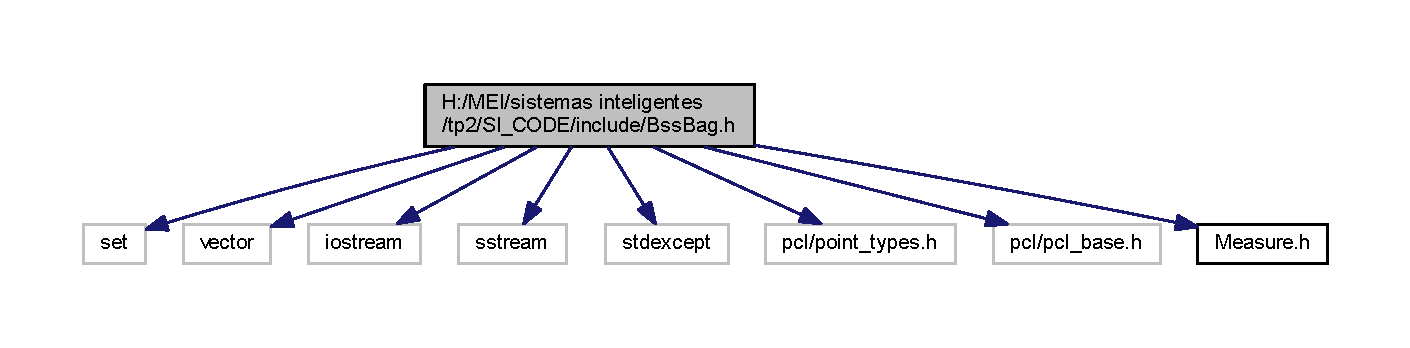
\includegraphics[width=350pt]{_bss_bag_8h__incl}
\end{center}
\end{figure}
This graph shows which files directly or indirectly include this file\+:
\nopagebreak
\begin{figure}[H]
\begin{center}
\leavevmode
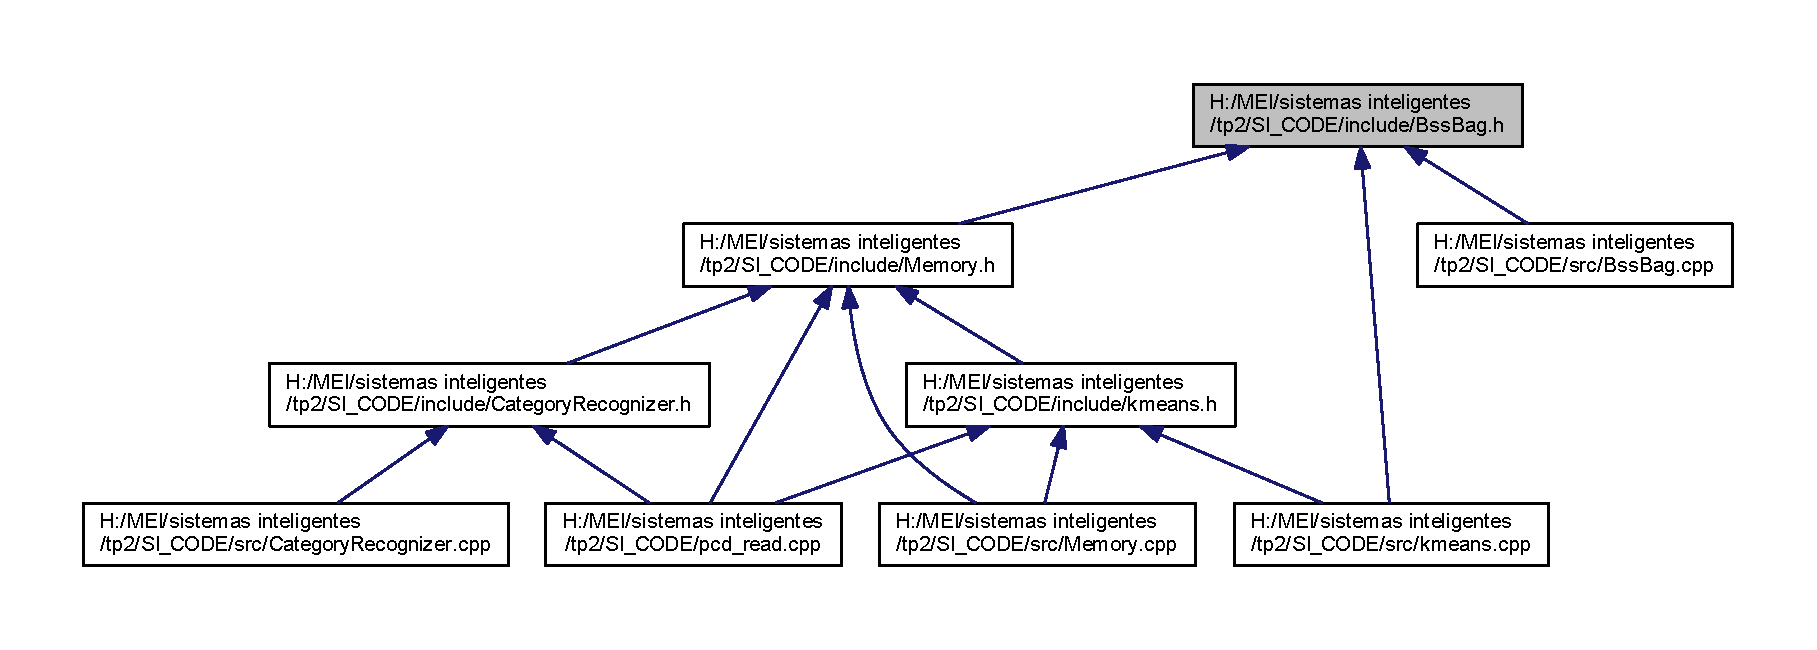
\includegraphics[width=350pt]{_bss_bag_8h__dep__incl}
\end{center}
\end{figure}
\subsection*{Classes}
\begin{DoxyCompactItemize}
\item 
class \hyperlink{class_bss_bag}{Bss\+Bag}
\begin{DoxyCompactList}\small\item\em Utility class to hold several mertadata about bss values. \end{DoxyCompactList}\end{DoxyCompactItemize}

\hypertarget{_category_8h}{}\section{H\+:/\+M\+E\+I/sistemas inteligentes/tp2/\+S\+I\+\_\+\+C\+O\+D\+E/include/\+Category.h File Reference}
\label{_category_8h}\index{H\+:/\+M\+E\+I/sistemas inteligentes/tp2/\+S\+I\+\_\+\+C\+O\+D\+E/include/\+Category.\+h@{H\+:/\+M\+E\+I/sistemas inteligentes/tp2/\+S\+I\+\_\+\+C\+O\+D\+E/include/\+Category.\+h}}
{\ttfamily \#include $<$set$>$}\newline
{\ttfamily \#include $<$vector$>$}\newline
{\ttfamily \#include $<$iostream$>$}\newline
{\ttfamily \#include $<$sstream$>$}\newline
{\ttfamily \#include $<$stdexcept$>$}\newline
{\ttfamily \#include $<$pcl/point\+\_\+types.\+h$>$}\newline
{\ttfamily \#include $<$pcl/pcl\+\_\+base.\+h$>$}\newline
{\ttfamily \#include \char`\"{}Measure.\+h\char`\"{}}\newline
{\ttfamily \#include $<$tr1/unordered\+\_\+set$>$}\newline
Include dependency graph for Category.\+h\+:
\nopagebreak
\begin{figure}[H]
\begin{center}
\leavevmode
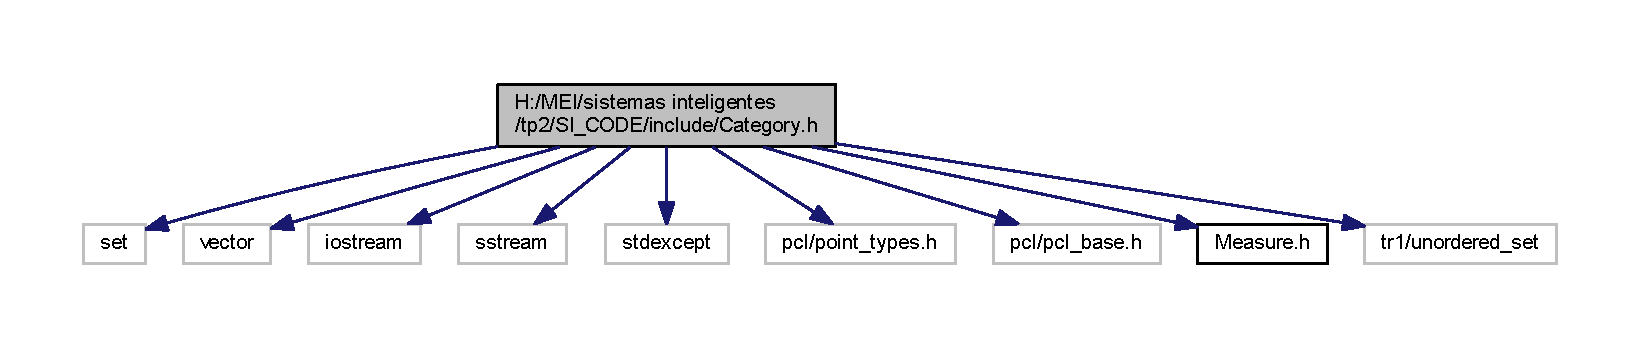
\includegraphics[width=350pt]{_category_8h__incl}
\end{center}
\end{figure}
This graph shows which files directly or indirectly include this file\+:
\nopagebreak
\begin{figure}[H]
\begin{center}
\leavevmode
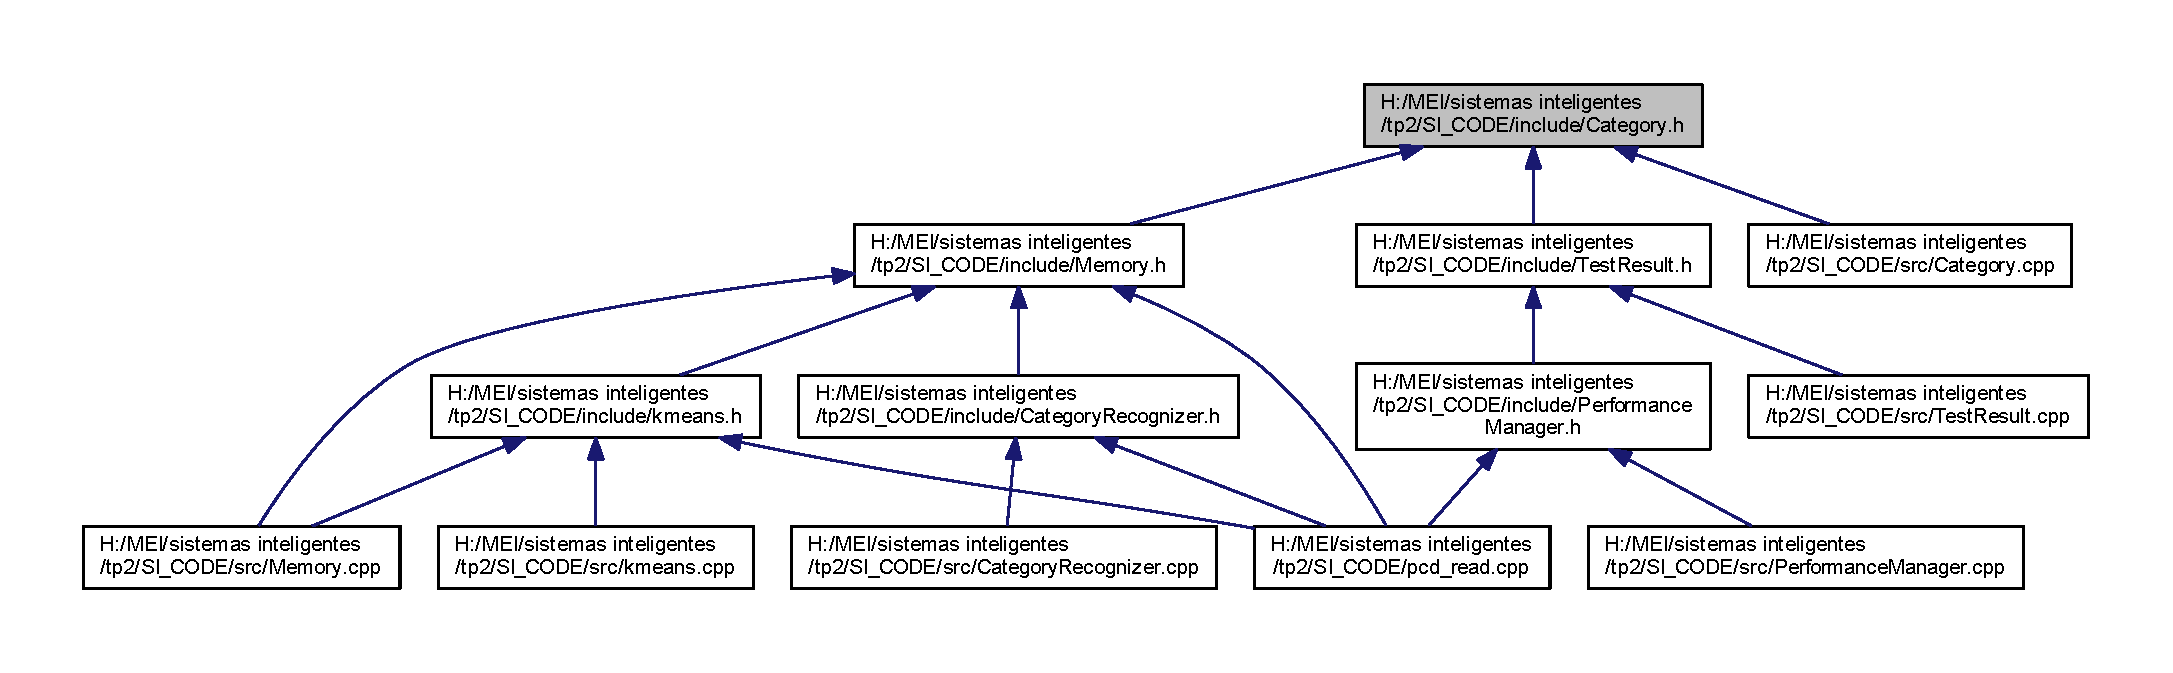
\includegraphics[width=350pt]{_category_8h__dep__incl}
\end{center}
\end{figure}
\subsection*{Classes}
\begin{DoxyCompactItemize}
\item 
class \hyperlink{class_category}{Category}
\begin{DoxyCompactList}\small\item\em Represents an object category, e.\+g., apple, bowl, bell-\/pepper, etc. \end{DoxyCompactList}\end{DoxyCompactItemize}

\hypertarget{_category_recognizer_8h}{}\section{H\+:/\+M\+E\+I/sistemas inteligentes/tp2/\+S\+I\+\_\+\+C\+O\+D\+E/include/\+Category\+Recognizer.h File Reference}
\label{_category_recognizer_8h}\index{H\+:/\+M\+E\+I/sistemas inteligentes/tp2/\+S\+I\+\_\+\+C\+O\+D\+E/include/\+Category\+Recognizer.\+h@{H\+:/\+M\+E\+I/sistemas inteligentes/tp2/\+S\+I\+\_\+\+C\+O\+D\+E/include/\+Category\+Recognizer.\+h}}
{\ttfamily \#include $<$map$>$}\newline
{\ttfamily \#include $<$stdexcept$>$}\newline
{\ttfamily \#include $<$pcl/point\+\_\+types.\+h$>$}\newline
{\ttfamily \#include $<$pcl/pcl\+\_\+base.\+h$>$}\newline
{\ttfamily \#include $<$pcl/common/point\+\_\+tests.\+h$>$}\newline
{\ttfamily \#include \char`\"{}Feature\+Metadata.\+h\char`\"{}}\newline
{\ttfamily \#include \char`\"{}Cluster.\+h\char`\"{}}\newline
{\ttfamily \#include \char`\"{}Searcher.\+h\char`\"{}}\newline
{\ttfamily \#include \char`\"{}Memory.\+h\char`\"{}}\newline
{\ttfamily \#include $<$tr1/unordered\+\_\+set$>$}\newline
{\ttfamily \#include $<$tr1/unordered\+\_\+map$>$}\newline
Include dependency graph for Category\+Recognizer.\+h\+:
\nopagebreak
\begin{figure}[H]
\begin{center}
\leavevmode
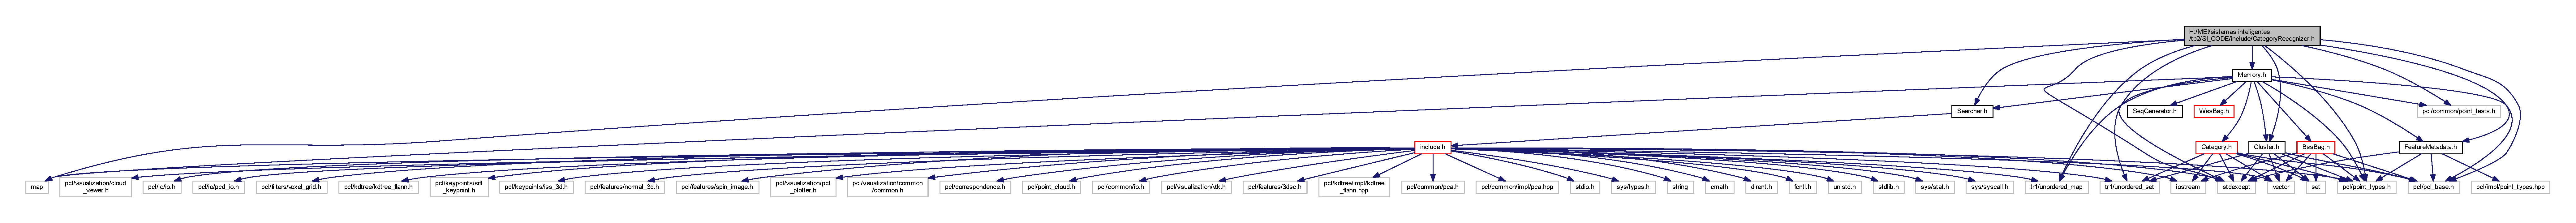
\includegraphics[width=350pt]{_category_recognizer_8h__incl}
\end{center}
\end{figure}
This graph shows which files directly or indirectly include this file\+:
\nopagebreak
\begin{figure}[H]
\begin{center}
\leavevmode
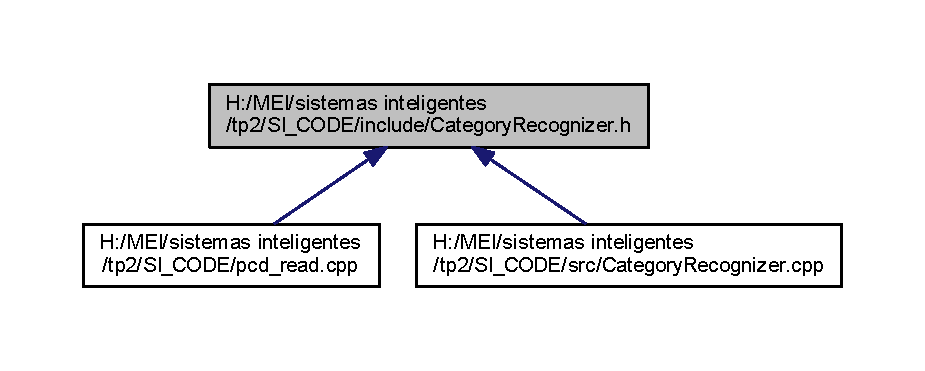
\includegraphics[width=350pt]{_category_recognizer_8h__dep__incl}
\end{center}
\end{figure}
\subsection*{Classes}
\begin{DoxyCompactItemize}
\item 
class \hyperlink{class_category_recognizer}{Category\+Recognizer}
\begin{DoxyCompactList}\small\item\em This class assigns an object view to a category, based on the euclidean distance between the object view histogram and the categories histgrams. \end{DoxyCompactList}\end{DoxyCompactItemize}

\hypertarget{_cluster_8h}{}\section{H\+:/\+M\+E\+I/sistemas inteligentes/tp2/\+S\+I\+\_\+\+C\+O\+D\+E/include/\+Cluster.h File Reference}
\label{_cluster_8h}\index{H\+:/\+M\+E\+I/sistemas inteligentes/tp2/\+S\+I\+\_\+\+C\+O\+D\+E/include/\+Cluster.\+h@{H\+:/\+M\+E\+I/sistemas inteligentes/tp2/\+S\+I\+\_\+\+C\+O\+D\+E/include/\+Cluster.\+h}}
{\ttfamily \#include $<$set$>$}\newline
{\ttfamily \#include $<$vector$>$}\newline
{\ttfamily \#include $<$pcl/point\+\_\+types.\+h$>$}\newline
{\ttfamily \#include $<$pcl/pcl\+\_\+base.\+h$>$}\newline
{\ttfamily \#include $<$stdexcept$>$}\newline
{\ttfamily \#include $<$tr1/unordered\+\_\+set$>$}\newline
Include dependency graph for Cluster.\+h\+:
\nopagebreak
\begin{figure}[H]
\begin{center}
\leavevmode
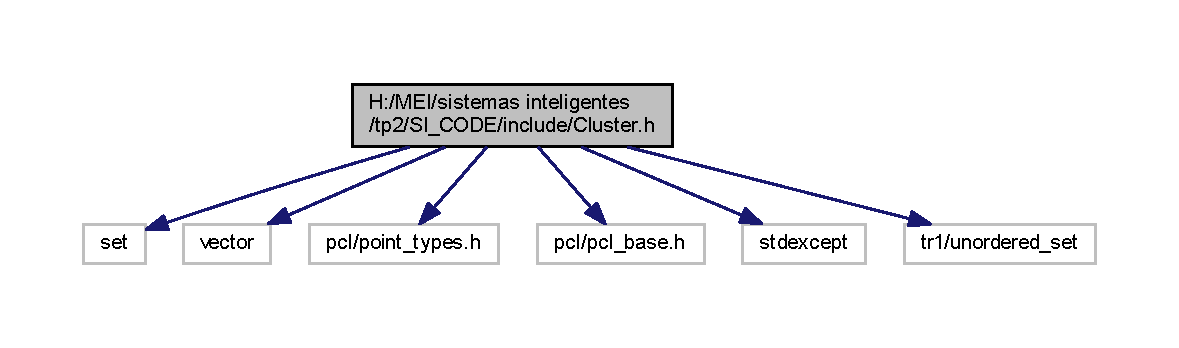
\includegraphics[width=350pt]{_cluster_8h__incl}
\end{center}
\end{figure}
This graph shows which files directly or indirectly include this file\+:
\nopagebreak
\begin{figure}[H]
\begin{center}
\leavevmode
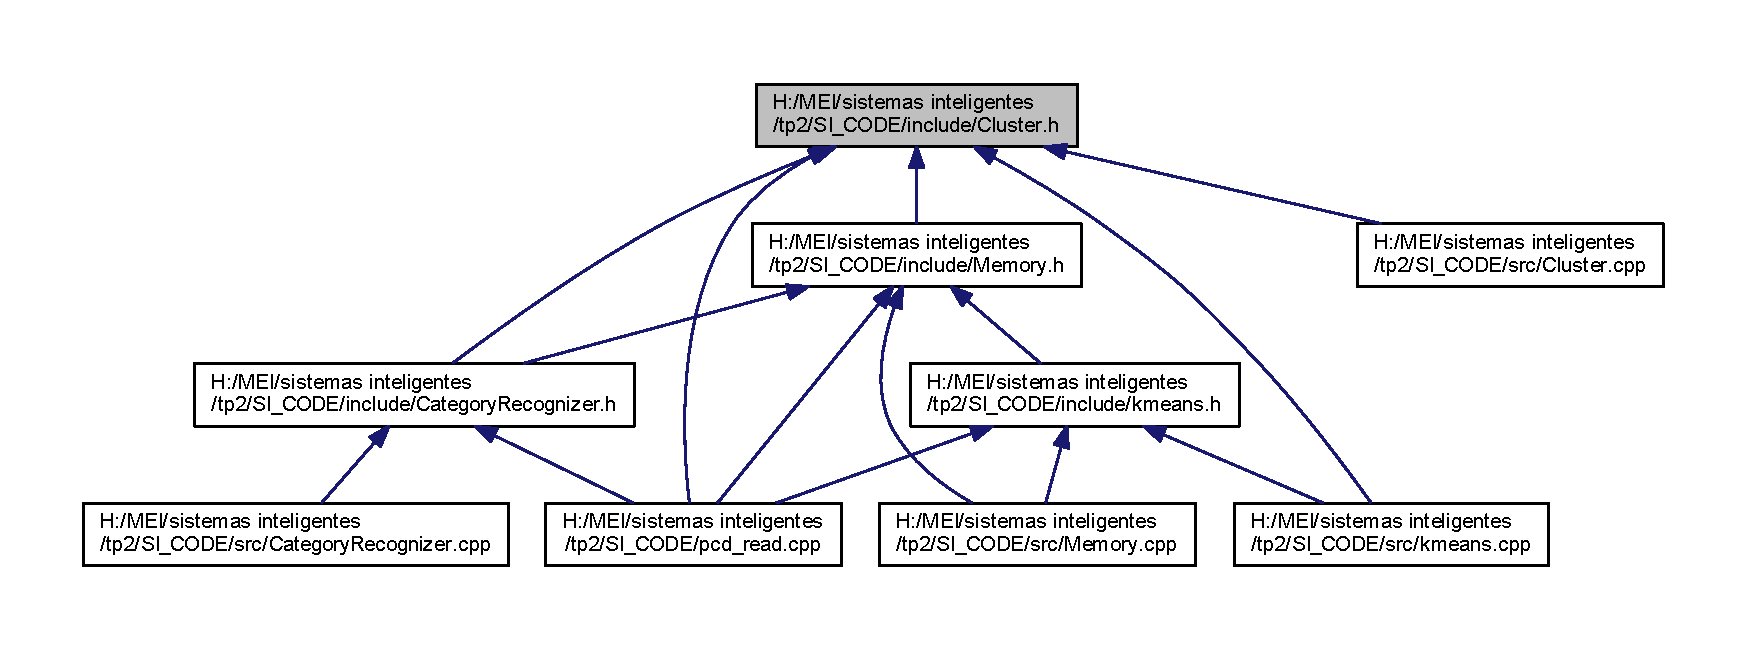
\includegraphics[width=350pt]{_cluster_8h__dep__incl}
\end{center}
\end{figure}
\subsection*{Classes}
\begin{DoxyCompactItemize}
\item 
class \hyperlink{class_cluster}{Cluster}
\begin{DoxyCompactList}\small\item\em Represents a cluster. \end{DoxyCompactList}\end{DoxyCompactItemize}

\hypertarget{_default_point_representation_8h}{}\section{H\+:/\+M\+E\+I/sistemas inteligentes/tp2/\+S\+I\+\_\+\+C\+O\+D\+E/include/\+Default\+Point\+Representation.h File Reference}
\label{_default_point_representation_8h}\index{H\+:/\+M\+E\+I/sistemas inteligentes/tp2/\+S\+I\+\_\+\+C\+O\+D\+E/include/\+Default\+Point\+Representation.\+h@{H\+:/\+M\+E\+I/sistemas inteligentes/tp2/\+S\+I\+\_\+\+C\+O\+D\+E/include/\+Default\+Point\+Representation.\+h}}
{\ttfamily \#include $<$pcl/point\+\_\+types.\+h$>$}\newline
Include dependency graph for Default\+Point\+Representation.\+h\+:
\nopagebreak
\begin{figure}[H]
\begin{center}
\leavevmode
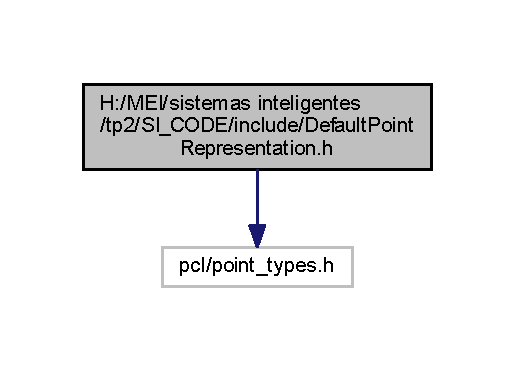
\includegraphics[width=247pt]{_default_point_representation_8h__incl}
\end{center}
\end{figure}
This graph shows which files directly or indirectly include this file\+:
\nopagebreak
\begin{figure}[H]
\begin{center}
\leavevmode
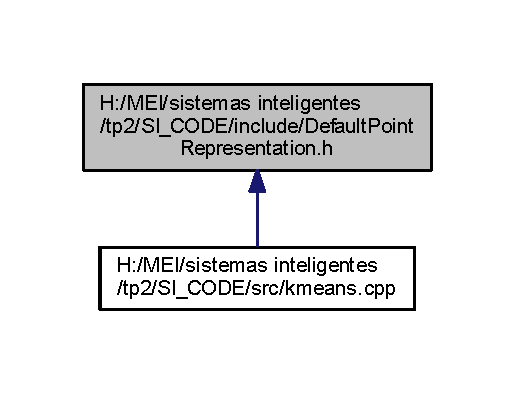
\includegraphics[width=247pt]{_default_point_representation_8h__dep__incl}
\end{center}
\end{figure}
\subsection*{Classes}
\begin{DoxyCompactItemize}
\item 
class \hyperlink{classpcl_1_1_default_point_representation_3_01_histogram_3_01153_01_4_01_4}{pcl\+::\+Default\+Point\+Representation$<$ Histogram$<$ 153 $>$ $>$}
\item 
class \hyperlink{classpcl_1_1_default_point_representation_3_01_histogram_3_01153_01_4_01_5_01_4}{pcl\+::\+Default\+Point\+Representation$<$ Histogram$<$ 153 $>$ $\ast$ $>$}
\end{DoxyCompactItemize}
\subsection*{Namespaces}
\begin{DoxyCompactItemize}
\item 
 \hyperlink{namespacepcl}{pcl}
\end{DoxyCompactItemize}

\hypertarget{_feature_extractor_8h}{}\section{H\+:/\+M\+E\+I/sistemas inteligentes/tp2/\+S\+I\+\_\+\+C\+O\+D\+E/include/\+Feature\+Extractor.h File Reference}
\label{_feature_extractor_8h}\index{H\+:/\+M\+E\+I/sistemas inteligentes/tp2/\+S\+I\+\_\+\+C\+O\+D\+E/include/\+Feature\+Extractor.\+h@{H\+:/\+M\+E\+I/sistemas inteligentes/tp2/\+S\+I\+\_\+\+C\+O\+D\+E/include/\+Feature\+Extractor.\+h}}
{\ttfamily \#include $<$include.\+h$>$}\newline
Include dependency graph for Feature\+Extractor.\+h\+:
\nopagebreak
\begin{figure}[H]
\begin{center}
\leavevmode
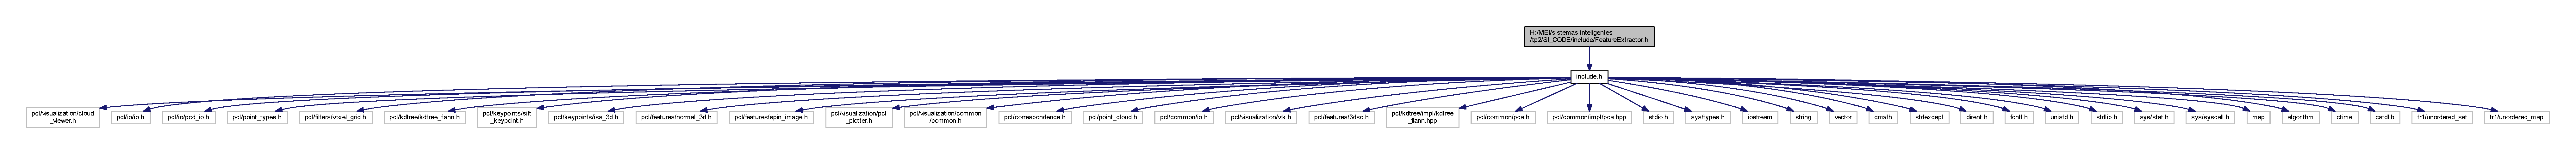
\includegraphics[width=350pt]{_feature_extractor_8h__incl}
\end{center}
\end{figure}
This graph shows which files directly or indirectly include this file\+:
\nopagebreak
\begin{figure}[H]
\begin{center}
\leavevmode
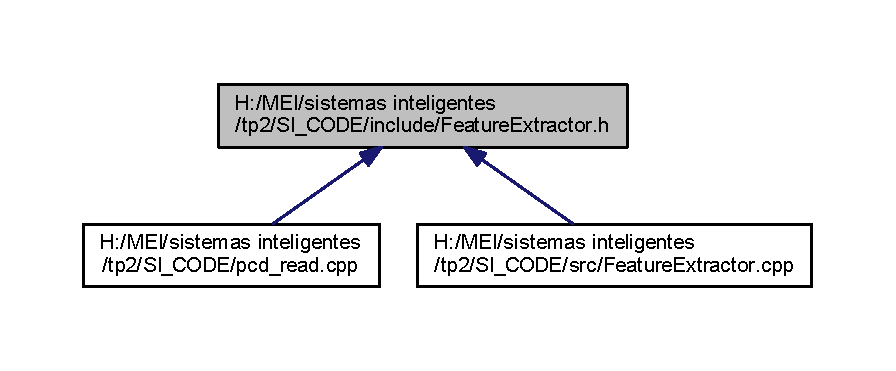
\includegraphics[width=350pt]{_feature_extractor_8h__dep__incl}
\end{center}
\end{figure}
\subsection*{Classes}
\begin{DoxyCompactItemize}
\item 
class \hyperlink{class_feature_extractor}{Feature\+Extractor}
\begin{DoxyCompactList}\small\item\em Functions to extract keypoints from a point cloud and compute spin images. \end{DoxyCompactList}\end{DoxyCompactItemize}

\hypertarget{_feature_metadata_8h}{}\section{H\+:/\+M\+E\+I/sistemas inteligentes/tp2/\+S\+I\+\_\+\+C\+O\+D\+E/include/\+Feature\+Metadata.h File Reference}
\label{_feature_metadata_8h}\index{H\+:/\+M\+E\+I/sistemas inteligentes/tp2/\+S\+I\+\_\+\+C\+O\+D\+E/include/\+Feature\+Metadata.\+h@{H\+:/\+M\+E\+I/sistemas inteligentes/tp2/\+S\+I\+\_\+\+C\+O\+D\+E/include/\+Feature\+Metadata.\+h}}
{\ttfamily \#include $<$pcl/point\+\_\+types.\+h$>$}\newline
{\ttfamily \#include $<$pcl/pcl\+\_\+base.\+h$>$}\newline
{\ttfamily \#include $<$pcl/impl/point\+\_\+types.\+hpp$>$}\newline
{\ttfamily \#include $<$stdexcept$>$}\newline
Include dependency graph for Feature\+Metadata.\+h\+:
\nopagebreak
\begin{figure}[H]
\begin{center}
\leavevmode
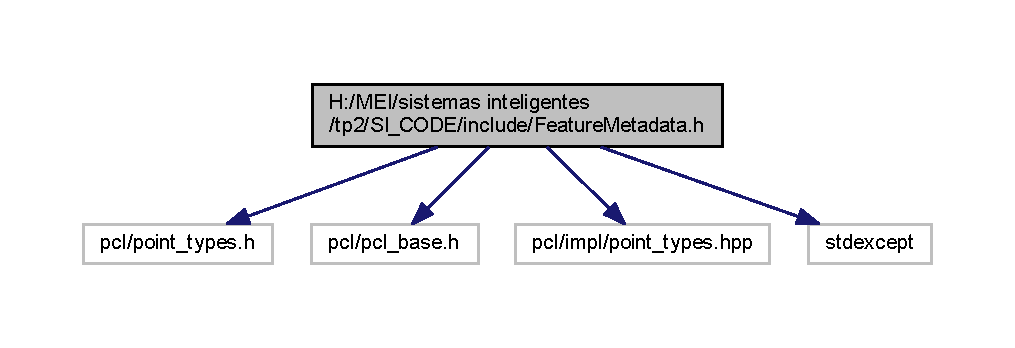
\includegraphics[width=350pt]{_feature_metadata_8h__incl}
\end{center}
\end{figure}
This graph shows which files directly or indirectly include this file\+:
\nopagebreak
\begin{figure}[H]
\begin{center}
\leavevmode
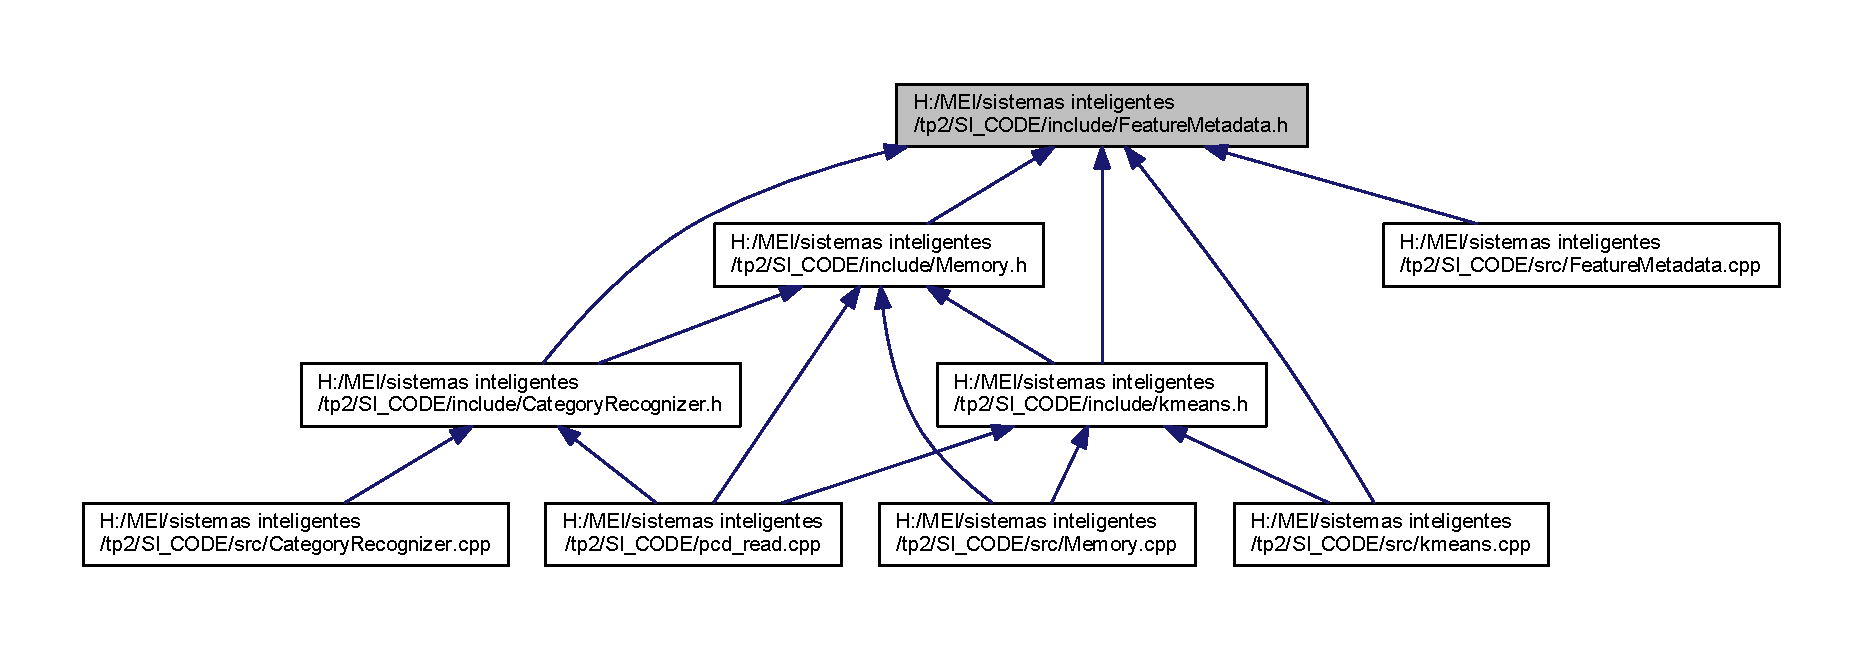
\includegraphics[width=350pt]{_feature_metadata_8h__dep__incl}
\end{center}
\end{figure}
\subsection*{Classes}
\begin{DoxyCompactItemize}
\item 
class \hyperlink{class_feature_metadata}{Feature\+Metadata}
\begin{DoxyCompactList}\small\item\em Holds metadata about a feature as well as the feature itself. \end{DoxyCompactList}\end{DoxyCompactItemize}

\hypertarget{include_8h}{}\section{H\+:/\+M\+E\+I/sistemas inteligentes/tp2/\+S\+I\+\_\+\+C\+O\+D\+E/include/include.h File Reference}
\label{include_8h}\index{H\+:/\+M\+E\+I/sistemas inteligentes/tp2/\+S\+I\+\_\+\+C\+O\+D\+E/include/include.\+h@{H\+:/\+M\+E\+I/sistemas inteligentes/tp2/\+S\+I\+\_\+\+C\+O\+D\+E/include/include.\+h}}
{\ttfamily \#include $<$pcl/visualization/cloud\+\_\+viewer.\+h$>$}\newline
{\ttfamily \#include $<$pcl/io/io.\+h$>$}\newline
{\ttfamily \#include $<$pcl/io/pcd\+\_\+io.\+h$>$}\newline
{\ttfamily \#include $<$pcl/point\+\_\+types.\+h$>$}\newline
{\ttfamily \#include $<$pcl/filters/voxel\+\_\+grid.\+h$>$}\newline
{\ttfamily \#include $<$pcl/kdtree/kdtree\+\_\+flann.\+h$>$}\newline
{\ttfamily \#include $<$pcl/keypoints/sift\+\_\+keypoint.\+h$>$}\newline
{\ttfamily \#include $<$pcl/keypoints/iss\+\_\+3d.\+h$>$}\newline
{\ttfamily \#include $<$pcl/features/normal\+\_\+3d.\+h$>$}\newline
{\ttfamily \#include $<$pcl/features/spin\+\_\+image.\+h$>$}\newline
{\ttfamily \#include $<$pcl/visualization/pcl\+\_\+plotter.\+h$>$}\newline
{\ttfamily \#include $<$pcl/visualization/common/common.\+h$>$}\newline
{\ttfamily \#include $<$pcl/correspondence.\+h$>$}\newline
{\ttfamily \#include $<$pcl/point\+\_\+cloud.\+h$>$}\newline
{\ttfamily \#include $<$pcl/common/io.\+h$>$}\newline
{\ttfamily \#include $<$pcl/visualization/vtk.\+h$>$}\newline
{\ttfamily \#include $<$pcl/features/3dsc.\+h$>$}\newline
{\ttfamily \#include $<$pcl/kdtree/impl/kdtree\+\_\+flann.\+hpp$>$}\newline
{\ttfamily \#include $<$pcl/common/pca.\+h$>$}\newline
{\ttfamily \#include $<$pcl/common/impl/pca.\+hpp$>$}\newline
{\ttfamily \#include $<$stdio.\+h$>$}\newline
{\ttfamily \#include $<$sys/types.\+h$>$}\newline
{\ttfamily \#include $<$iostream$>$}\newline
{\ttfamily \#include $<$string$>$}\newline
{\ttfamily \#include $<$vector$>$}\newline
{\ttfamily \#include $<$cmath$>$}\newline
{\ttfamily \#include $<$stdexcept$>$}\newline
{\ttfamily \#include $<$dirent.\+h$>$}\newline
{\ttfamily \#include $<$fcntl.\+h$>$}\newline
{\ttfamily \#include $<$unistd.\+h$>$}\newline
{\ttfamily \#include $<$stdlib.\+h$>$}\newline
{\ttfamily \#include $<$sys/stat.\+h$>$}\newline
{\ttfamily \#include $<$sys/syscall.\+h$>$}\newline
{\ttfamily \#include $<$map$>$}\newline
{\ttfamily \#include $<$algorithm$>$}\newline
{\ttfamily \#include $<$ctime$>$}\newline
{\ttfamily \#include $<$cstdlib$>$}\newline
{\ttfamily \#include $<$tr1/unordered\+\_\+set$>$}\newline
{\ttfamily \#include $<$tr1/unordered\+\_\+map$>$}\newline
Include dependency graph for include.\+h\+:
\nopagebreak
\begin{figure}[H]
\begin{center}
\leavevmode
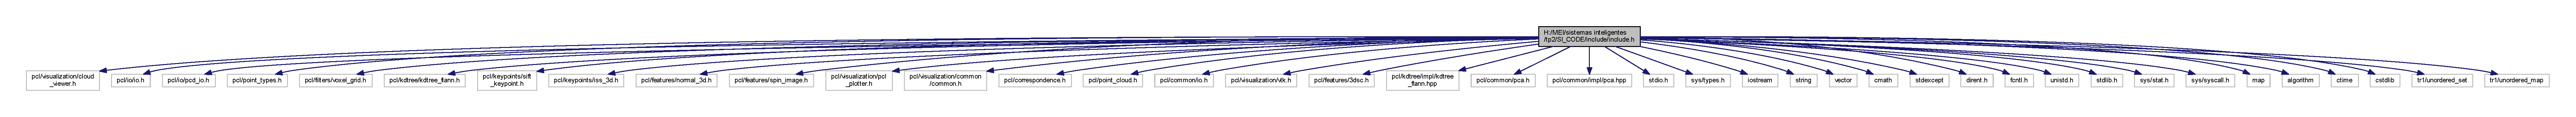
\includegraphics[width=350pt]{include_8h__incl}
\end{center}
\end{figure}
This graph shows which files directly or indirectly include this file\+:
\nopagebreak
\begin{figure}[H]
\begin{center}
\leavevmode
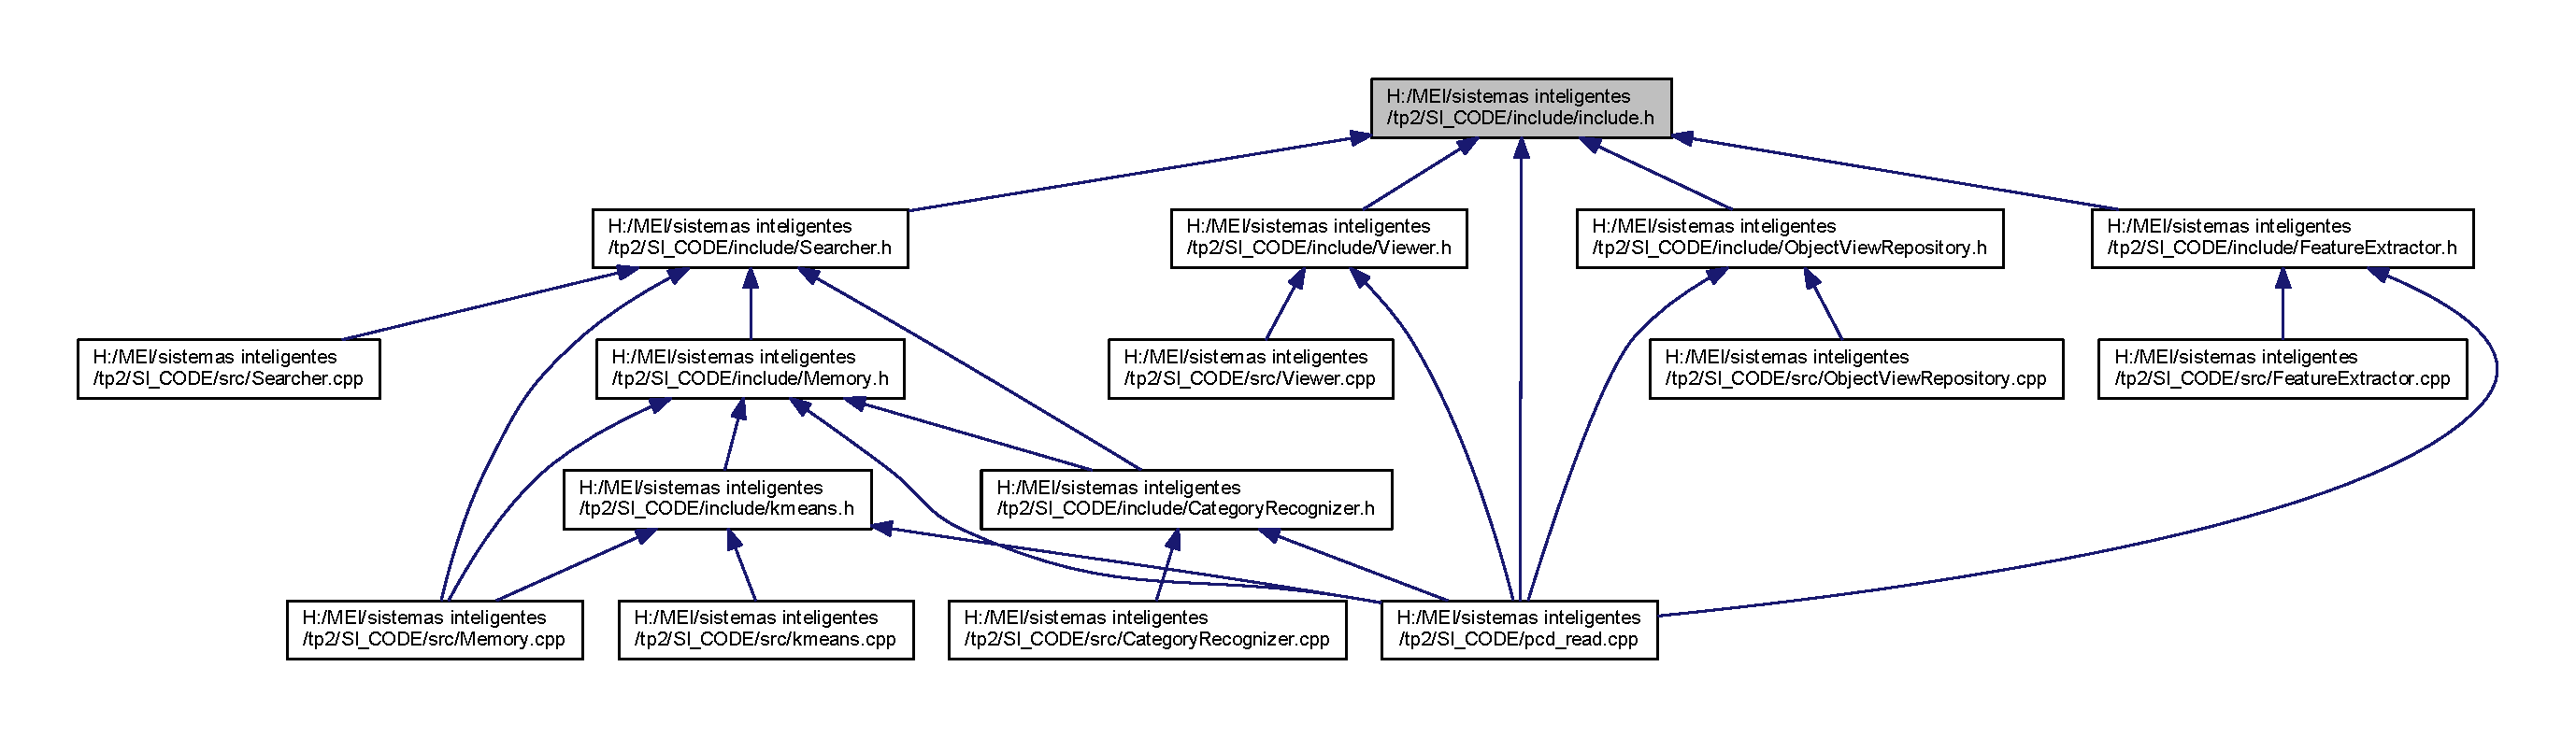
\includegraphics[width=350pt]{include_8h__dep__incl}
\end{center}
\end{figure}
\subsection*{Classes}
\begin{DoxyCompactItemize}
\item 
struct \hyperlink{structlinux__dirent}{linux\+\_\+dirent}
\end{DoxyCompactItemize}
\subsection*{Macros}
\begin{DoxyCompactItemize}
\item 
\#define \hyperlink{include_8h_a6821bafc3c88dfb2e433a095df9940c6}{B\+U\+F\+\_\+\+S\+I\+ZE}~1024
\item 
\#define \hyperlink{include_8h_a9d1a12bca0d256595c65ca333f66d421}{L\+E\+A\+R\+N\+I\+NG}~1
\item 
\#define \hyperlink{include_8h_a696dfa95dff38765b2a37930ff408ea1}{T\+R\+A\+I\+N\+I\+NG}~2
\end{DoxyCompactItemize}
\subsection*{Typedefs}
\begin{DoxyCompactItemize}
\item 
typedef Histogram$<$ 153 $>$ \hyperlink{include_8h_ab79ade12a22a8e5e2864650f820e9c6f}{Spin\+Image}
\item 
typedef Point\+X\+Y\+Z\+R\+GB \hyperlink{include_8h_a6ca7710b84e9152e036423253ffc1ae7}{PointT}
\end{DoxyCompactItemize}


\subsection{Macro Definition Documentation}
\mbox{\Hypertarget{include_8h_a6821bafc3c88dfb2e433a095df9940c6}\label{include_8h_a6821bafc3c88dfb2e433a095df9940c6}} 
\index{include.\+h@{include.\+h}!B\+U\+F\+\_\+\+S\+I\+ZE@{B\+U\+F\+\_\+\+S\+I\+ZE}}
\index{B\+U\+F\+\_\+\+S\+I\+ZE@{B\+U\+F\+\_\+\+S\+I\+ZE}!include.\+h@{include.\+h}}
\subsubsection{\texorpdfstring{B\+U\+F\+\_\+\+S\+I\+ZE}{BUF\_SIZE}}
{\footnotesize\ttfamily \#define B\+U\+F\+\_\+\+S\+I\+ZE~1024}



Definition at line 67 of file include.\+h.

\mbox{\Hypertarget{include_8h_a9d1a12bca0d256595c65ca333f66d421}\label{include_8h_a9d1a12bca0d256595c65ca333f66d421}} 
\index{include.\+h@{include.\+h}!L\+E\+A\+R\+N\+I\+NG@{L\+E\+A\+R\+N\+I\+NG}}
\index{L\+E\+A\+R\+N\+I\+NG@{L\+E\+A\+R\+N\+I\+NG}!include.\+h@{include.\+h}}
\subsubsection{\texorpdfstring{L\+E\+A\+R\+N\+I\+NG}{LEARNING}}
{\footnotesize\ttfamily \#define L\+E\+A\+R\+N\+I\+NG~1}



Definition at line 68 of file include.\+h.

\mbox{\Hypertarget{include_8h_a696dfa95dff38765b2a37930ff408ea1}\label{include_8h_a696dfa95dff38765b2a37930ff408ea1}} 
\index{include.\+h@{include.\+h}!T\+R\+A\+I\+N\+I\+NG@{T\+R\+A\+I\+N\+I\+NG}}
\index{T\+R\+A\+I\+N\+I\+NG@{T\+R\+A\+I\+N\+I\+NG}!include.\+h@{include.\+h}}
\subsubsection{\texorpdfstring{T\+R\+A\+I\+N\+I\+NG}{TRAINING}}
{\footnotesize\ttfamily \#define T\+R\+A\+I\+N\+I\+NG~2}



Definition at line 69 of file include.\+h.



\subsection{Typedef Documentation}
\mbox{\Hypertarget{include_8h_a6ca7710b84e9152e036423253ffc1ae7}\label{include_8h_a6ca7710b84e9152e036423253ffc1ae7}} 
\index{include.\+h@{include.\+h}!PointT@{PointT}}
\index{PointT@{PointT}!include.\+h@{include.\+h}}
\subsubsection{\texorpdfstring{PointT}{PointT}}
{\footnotesize\ttfamily typedef Point\+X\+Y\+Z\+R\+GB \hyperlink{include_8h_a6ca7710b84e9152e036423253ffc1ae7}{PointT}}



Definition at line 58 of file include.\+h.

\mbox{\Hypertarget{include_8h_ab79ade12a22a8e5e2864650f820e9c6f}\label{include_8h_ab79ade12a22a8e5e2864650f820e9c6f}} 
\index{include.\+h@{include.\+h}!Spin\+Image@{Spin\+Image}}
\index{Spin\+Image@{Spin\+Image}!include.\+h@{include.\+h}}
\subsubsection{\texorpdfstring{Spin\+Image}{SpinImage}}
{\footnotesize\ttfamily typedef Histogram$<$153$>$ \hyperlink{include_8h_ab79ade12a22a8e5e2864650f820e9c6f}{Spin\+Image}}



Definition at line 57 of file include.\+h.


\hypertarget{kmeans_8h}{}\section{H\+:/\+M\+E\+I/sistemas inteligentes/tp2/\+S\+I\+\_\+\+C\+O\+D\+E/include/kmeans.h File Reference}
\label{kmeans_8h}\index{H\+:/\+M\+E\+I/sistemas inteligentes/tp2/\+S\+I\+\_\+\+C\+O\+D\+E/include/kmeans.\+h@{H\+:/\+M\+E\+I/sistemas inteligentes/tp2/\+S\+I\+\_\+\+C\+O\+D\+E/include/kmeans.\+h}}
{\ttfamily \#include $<$map$>$}\newline
{\ttfamily \#include $<$string$>$}\newline
{\ttfamily \#include $<$vector$>$}\newline
{\ttfamily \#include $<$pcl/point\+\_\+types.\+h$>$}\newline
{\ttfamily \#include $<$pcl/pcl\+\_\+base.\+h$>$}\newline
{\ttfamily \#include \char`\"{}Memory.\+h\char`\"{}}\newline
{\ttfamily \#include \char`\"{}Feature\+Metadata.\+h\char`\"{}}\newline
{\ttfamily \#include $<$tr1/unordered\+\_\+map$>$}\newline
Include dependency graph for kmeans.\+h\+:
\nopagebreak
\begin{figure}[H]
\begin{center}
\leavevmode
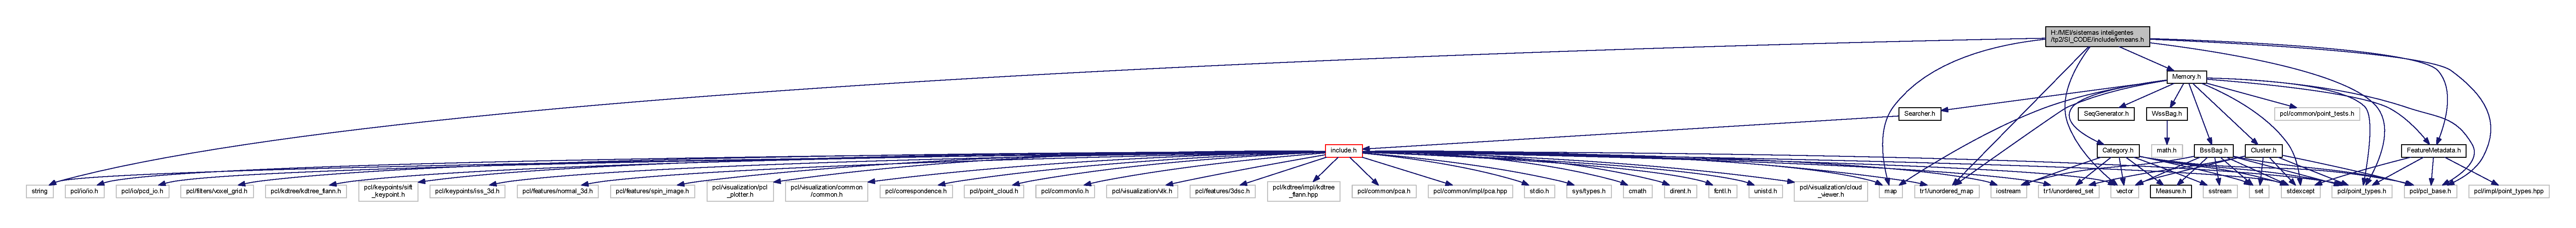
\includegraphics[width=350pt]{kmeans_8h__incl}
\end{center}
\end{figure}
This graph shows which files directly or indirectly include this file\+:
\nopagebreak
\begin{figure}[H]
\begin{center}
\leavevmode
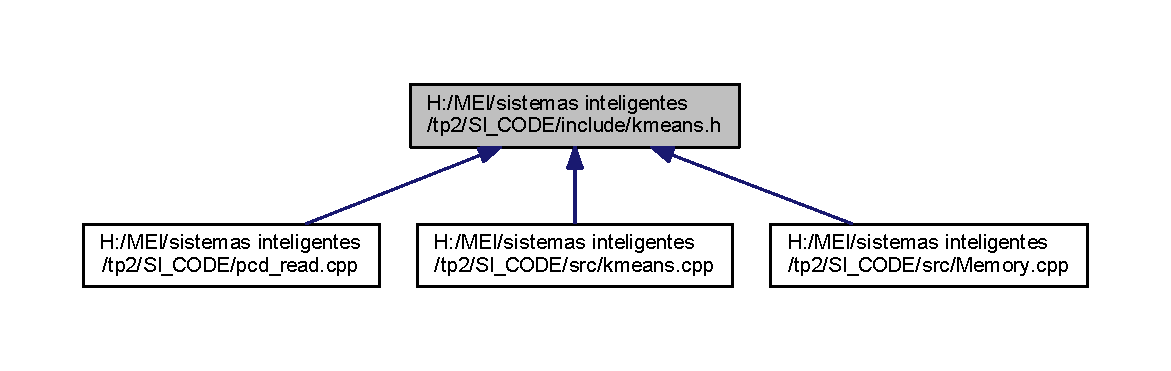
\includegraphics[width=350pt]{kmeans_8h__dep__incl}
\end{center}
\end{figure}
\subsection*{Classes}
\begin{DoxyCompactItemize}
\item 
class \hyperlink{class_k_means}{K\+Means}
\begin{DoxyCompactList}\small\item\em A custom implementation of Kmeans. \end{DoxyCompactList}\end{DoxyCompactItemize}

\hypertarget{_measure_8h}{}\section{H\+:/\+M\+E\+I/sistemas inteligentes/tp2/\+S\+I\+\_\+\+C\+O\+D\+E/include/\+Measure.h File Reference}
\label{_measure_8h}\index{H\+:/\+M\+E\+I/sistemas inteligentes/tp2/\+S\+I\+\_\+\+C\+O\+D\+E/include/\+Measure.\+h@{H\+:/\+M\+E\+I/sistemas inteligentes/tp2/\+S\+I\+\_\+\+C\+O\+D\+E/include/\+Measure.\+h}}
This graph shows which files directly or indirectly include this file\+:
\nopagebreak
\begin{figure}[H]
\begin{center}
\leavevmode
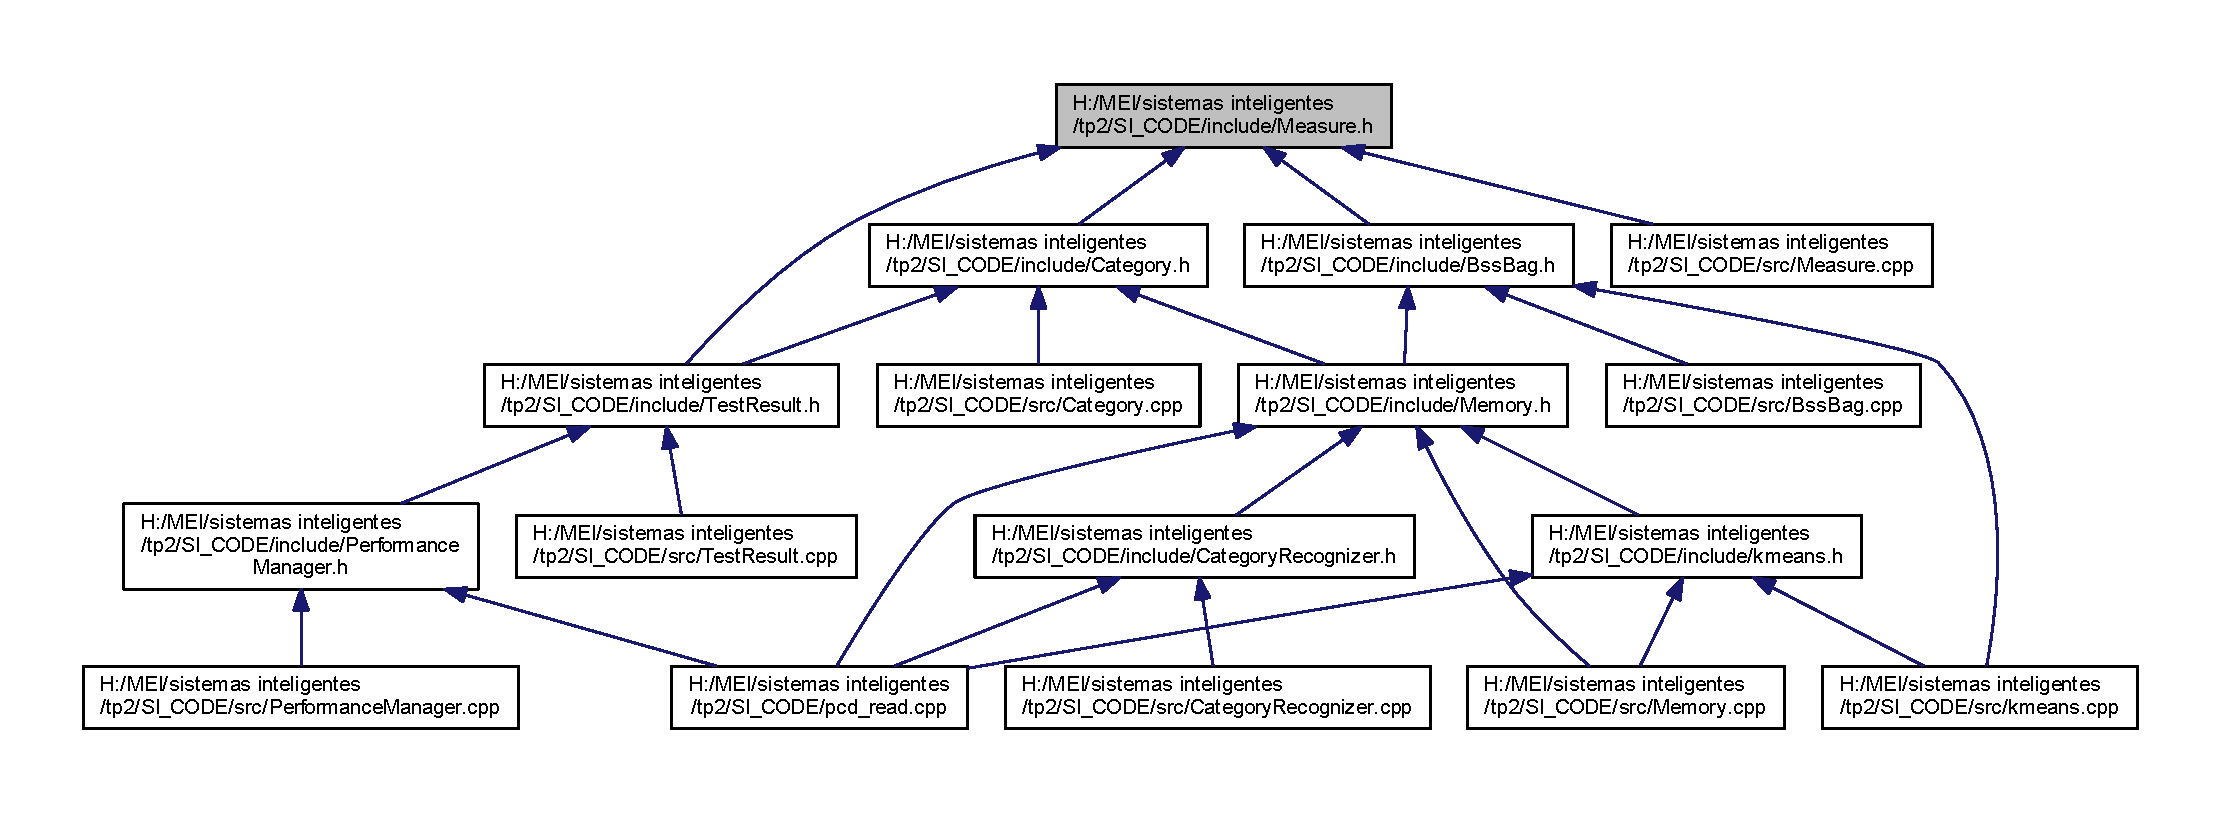
\includegraphics[width=350pt]{_measure_8h__dep__incl}
\end{center}
\end{figure}
\subsection*{Classes}
\begin{DoxyCompactItemize}
\item 
class \hyperlink{class_measure}{Measure}
\begin{DoxyCompactList}\small\item\em A class used to measure the performance of the application assigning object views to categories. Use to hold the results for a specific category. \end{DoxyCompactList}\end{DoxyCompactItemize}

\hypertarget{_memory_8h}{}\section{H\+:/\+M\+E\+I/sistemas inteligentes/tp2/\+S\+I\+\_\+\+C\+O\+D\+E/include/\+Memory.h File Reference}
\label{_memory_8h}\index{H\+:/\+M\+E\+I/sistemas inteligentes/tp2/\+S\+I\+\_\+\+C\+O\+D\+E/include/\+Memory.\+h@{H\+:/\+M\+E\+I/sistemas inteligentes/tp2/\+S\+I\+\_\+\+C\+O\+D\+E/include/\+Memory.\+h}}
{\ttfamily \#include $<$map$>$}\newline
{\ttfamily \#include $<$pcl/point\+\_\+types.\+h$>$}\newline
{\ttfamily \#include $<$pcl/pcl\+\_\+base.\+h$>$}\newline
{\ttfamily \#include $<$pcl/common/point\+\_\+tests.\+h$>$}\newline
{\ttfamily \#include \char`\"{}Feature\+Metadata.\+h\char`\"{}}\newline
{\ttfamily \#include \char`\"{}Cluster.\+h\char`\"{}}\newline
{\ttfamily \#include \char`\"{}Searcher.\+h\char`\"{}}\newline
{\ttfamily \#include \char`\"{}Category.\+h\char`\"{}}\newline
{\ttfamily \#include \char`\"{}Seq\+Generator.\+h\char`\"{}}\newline
{\ttfamily \#include \char`\"{}Wss\+Bag.\+h\char`\"{}}\newline
{\ttfamily \#include \char`\"{}Bss\+Bag.\+h\char`\"{}}\newline
{\ttfamily \#include $<$stdexcept$>$}\newline
{\ttfamily \#include $<$tr1/unordered\+\_\+map$>$}\newline
Include dependency graph for Memory.\+h\+:
\nopagebreak
\begin{figure}[H]
\begin{center}
\leavevmode
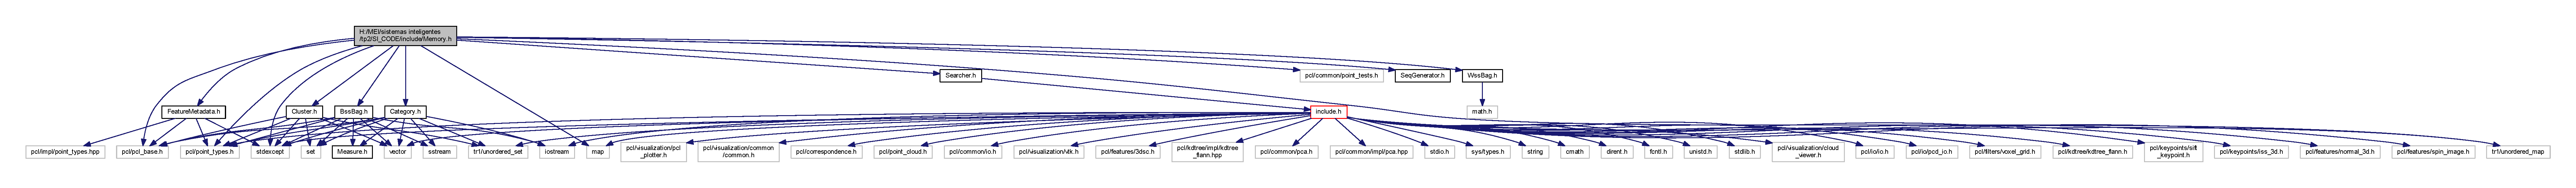
\includegraphics[width=350pt]{_memory_8h__incl}
\end{center}
\end{figure}
This graph shows which files directly or indirectly include this file\+:
\nopagebreak
\begin{figure}[H]
\begin{center}
\leavevmode
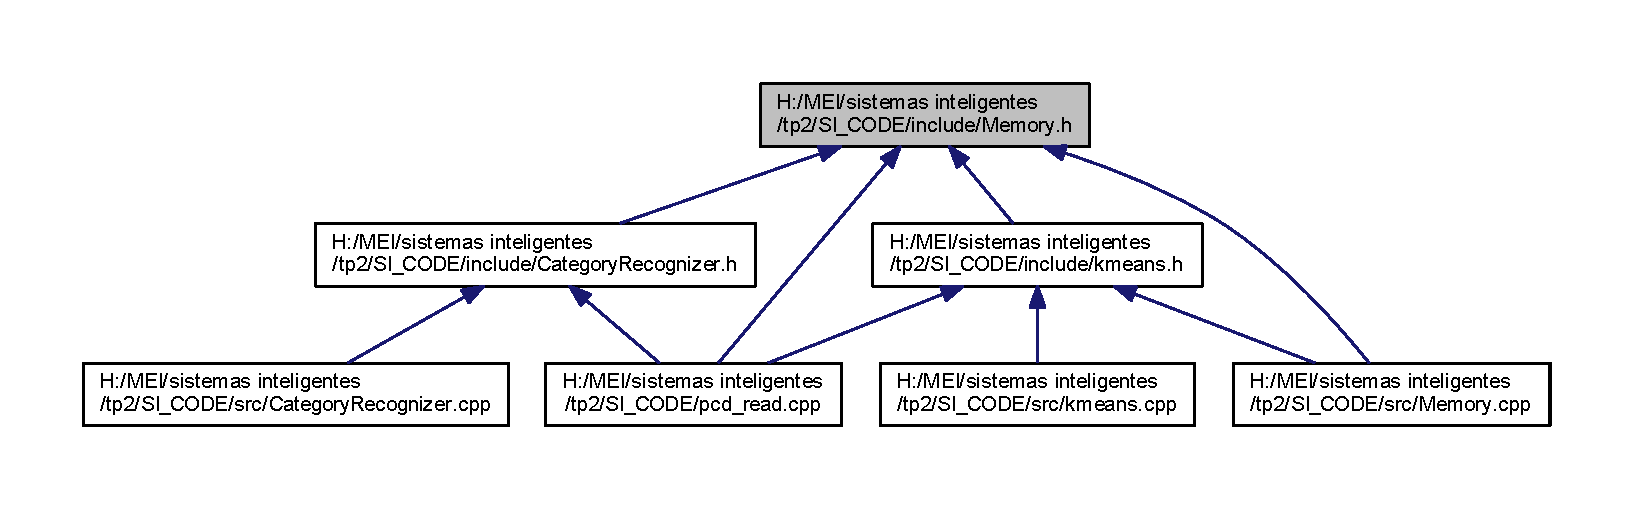
\includegraphics[width=350pt]{_memory_8h__dep__incl}
\end{center}
\end{figure}
\subsection*{Classes}
\begin{DoxyCompactItemize}
\item 
class \hyperlink{class_memory}{Memory}
\begin{DoxyCompactList}\small\item\em Main structure of the application. Holds the applications\textquotesingle{} memory. \end{DoxyCompactList}\item 
struct \hyperlink{struct_memory_1_1_category_view_distance}{Memory\+::\+Category\+View\+Distance}
\begin{DoxyCompactList}\small\item\em Auxiliar data structure to hold the distances between a specific object view and the categories. The distance is the euclidean distance between the respective histograms. \end{DoxyCompactList}\item 
struct \hyperlink{structdescending}{descending}
\begin{DoxyCompactList}\small\item\em Operator used with std\+:sort to sort a vector$<$pair$<$int, float$>$ $>$ by the value of the pair (the second argument of the pair, the float) in descending order. \end{DoxyCompactList}\end{DoxyCompactItemize}

\hypertarget{_object_view_repository_8h}{}\section{H\+:/\+M\+E\+I/sistemas inteligentes/tp2/\+S\+I\+\_\+\+C\+O\+D\+E/include/\+Object\+View\+Repository.h File Reference}
\label{_object_view_repository_8h}\index{H\+:/\+M\+E\+I/sistemas inteligentes/tp2/\+S\+I\+\_\+\+C\+O\+D\+E/include/\+Object\+View\+Repository.\+h@{H\+:/\+M\+E\+I/sistemas inteligentes/tp2/\+S\+I\+\_\+\+C\+O\+D\+E/include/\+Object\+View\+Repository.\+h}}
{\ttfamily \#include $<$include.\+h$>$}\newline
Include dependency graph for Object\+View\+Repository.\+h\+:
\nopagebreak
\begin{figure}[H]
\begin{center}
\leavevmode
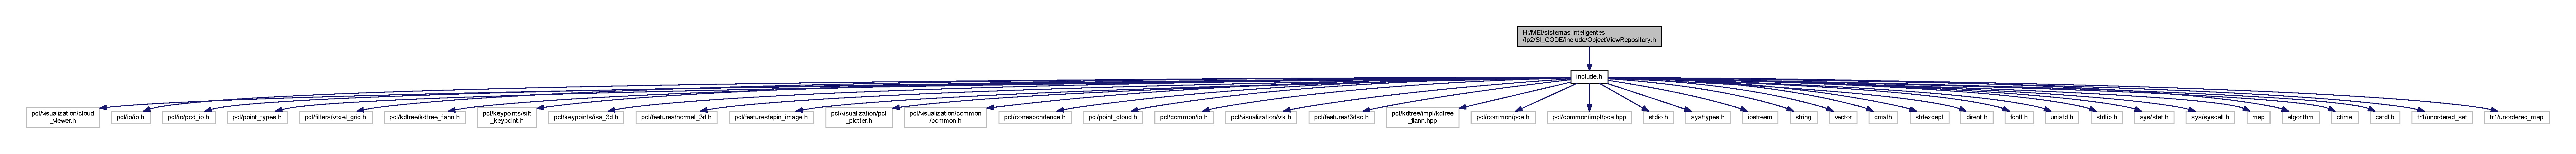
\includegraphics[width=350pt]{_object_view_repository_8h__incl}
\end{center}
\end{figure}
This graph shows which files directly or indirectly include this file\+:
\nopagebreak
\begin{figure}[H]
\begin{center}
\leavevmode
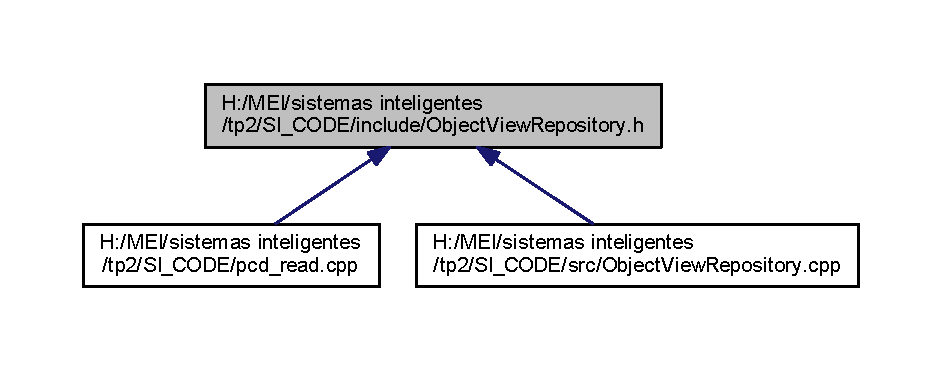
\includegraphics[width=350pt]{_object_view_repository_8h__dep__incl}
\end{center}
\end{figure}
\subsection*{Classes}
\begin{DoxyCompactItemize}
\item 
class \hyperlink{class_object_view_repository}{Object\+View\+Repository}
\begin{DoxyCompactList}\small\item\em Loads point clouds from a given directory. Also provides shuffle for random point cloud viewing. This class should not be reused because some paremeter are shared and must be re-\/initialized properly! \end{DoxyCompactList}\end{DoxyCompactItemize}

\hypertarget{_performance_manager_8h}{}\section{H\+:/\+M\+E\+I/sistemas inteligentes/tp2/\+S\+I\+\_\+\+C\+O\+D\+E/include/\+Performance\+Manager.h File Reference}
\label{_performance_manager_8h}\index{H\+:/\+M\+E\+I/sistemas inteligentes/tp2/\+S\+I\+\_\+\+C\+O\+D\+E/include/\+Performance\+Manager.\+h@{H\+:/\+M\+E\+I/sistemas inteligentes/tp2/\+S\+I\+\_\+\+C\+O\+D\+E/include/\+Performance\+Manager.\+h}}
{\ttfamily \#include $<$vector$>$}\newline
{\ttfamily \#include \char`\"{}Test\+Result.\+h\char`\"{}}\newline
Include dependency graph for Performance\+Manager.\+h\+:
\nopagebreak
\begin{figure}[H]
\begin{center}
\leavevmode
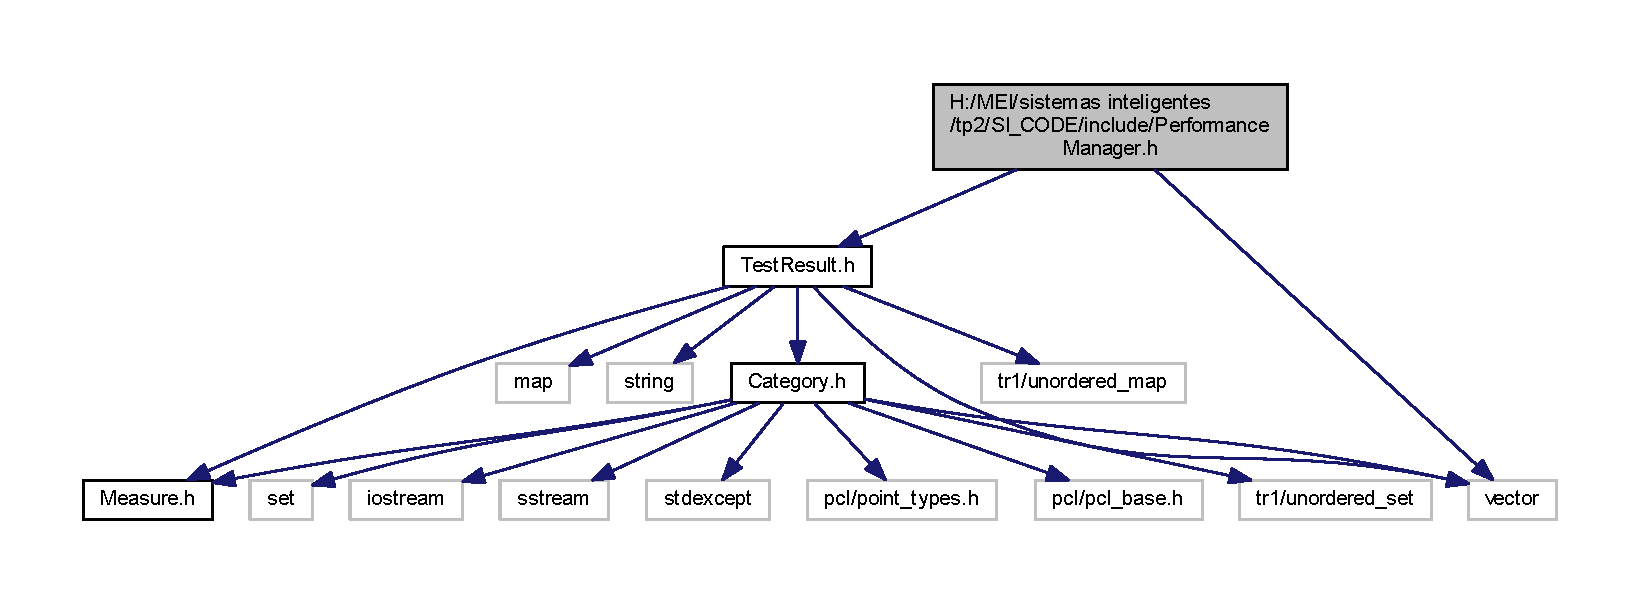
\includegraphics[width=350pt]{_performance_manager_8h__incl}
\end{center}
\end{figure}
This graph shows which files directly or indirectly include this file\+:
\nopagebreak
\begin{figure}[H]
\begin{center}
\leavevmode
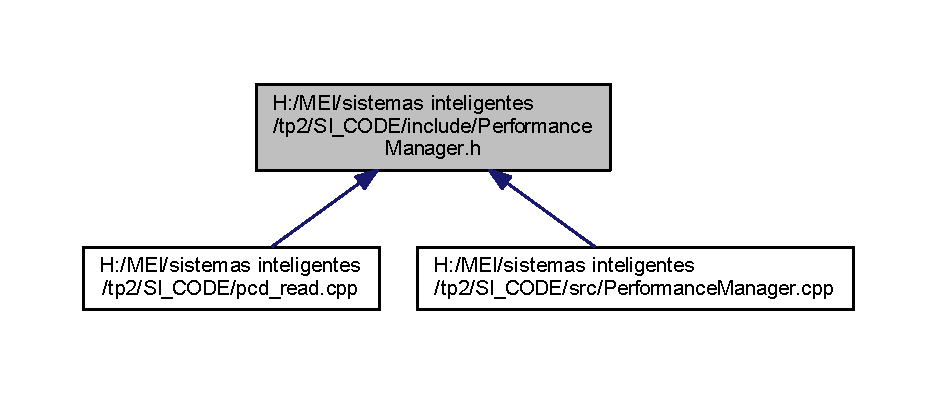
\includegraphics[width=350pt]{_performance_manager_8h__dep__incl}
\end{center}
\end{figure}
\subsection*{Classes}
\begin{DoxyCompactItemize}
\item 
class \hyperlink{class_performance_manager}{Performance\+Manager}
\begin{DoxyCompactList}\small\item\em A class to handle performance results. \end{DoxyCompactList}\item 
struct \hyperlink{struct_performance_manager_1_1_average_results}{Performance\+Manager\+::\+Average\+Results}
\end{DoxyCompactItemize}

\hypertarget{_searcher_8h}{}\section{H\+:/\+M\+E\+I/sistemas inteligentes/tp2/\+S\+I\+\_\+\+C\+O\+D\+E/include/\+Searcher.h File Reference}
\label{_searcher_8h}\index{H\+:/\+M\+E\+I/sistemas inteligentes/tp2/\+S\+I\+\_\+\+C\+O\+D\+E/include/\+Searcher.\+h@{H\+:/\+M\+E\+I/sistemas inteligentes/tp2/\+S\+I\+\_\+\+C\+O\+D\+E/include/\+Searcher.\+h}}
{\ttfamily \#include $<$include.\+h$>$}\newline
Include dependency graph for Searcher.\+h\+:
\nopagebreak
\begin{figure}[H]
\begin{center}
\leavevmode
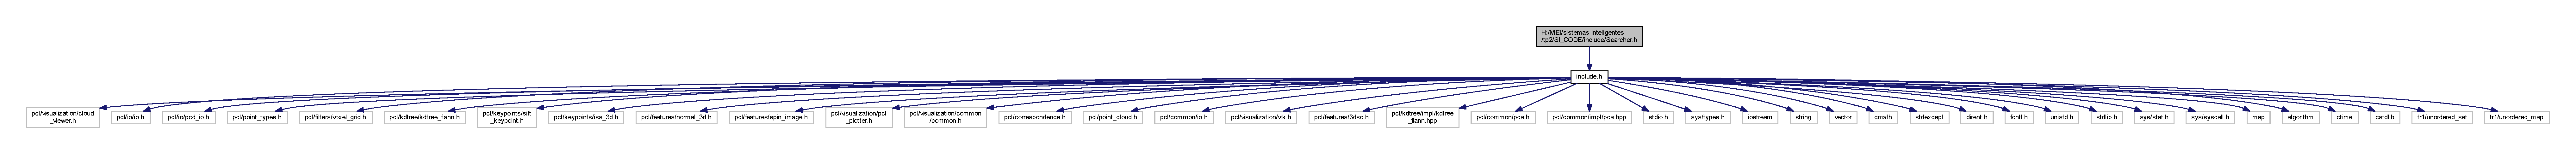
\includegraphics[width=350pt]{_searcher_8h__incl}
\end{center}
\end{figure}
This graph shows which files directly or indirectly include this file\+:
\nopagebreak
\begin{figure}[H]
\begin{center}
\leavevmode
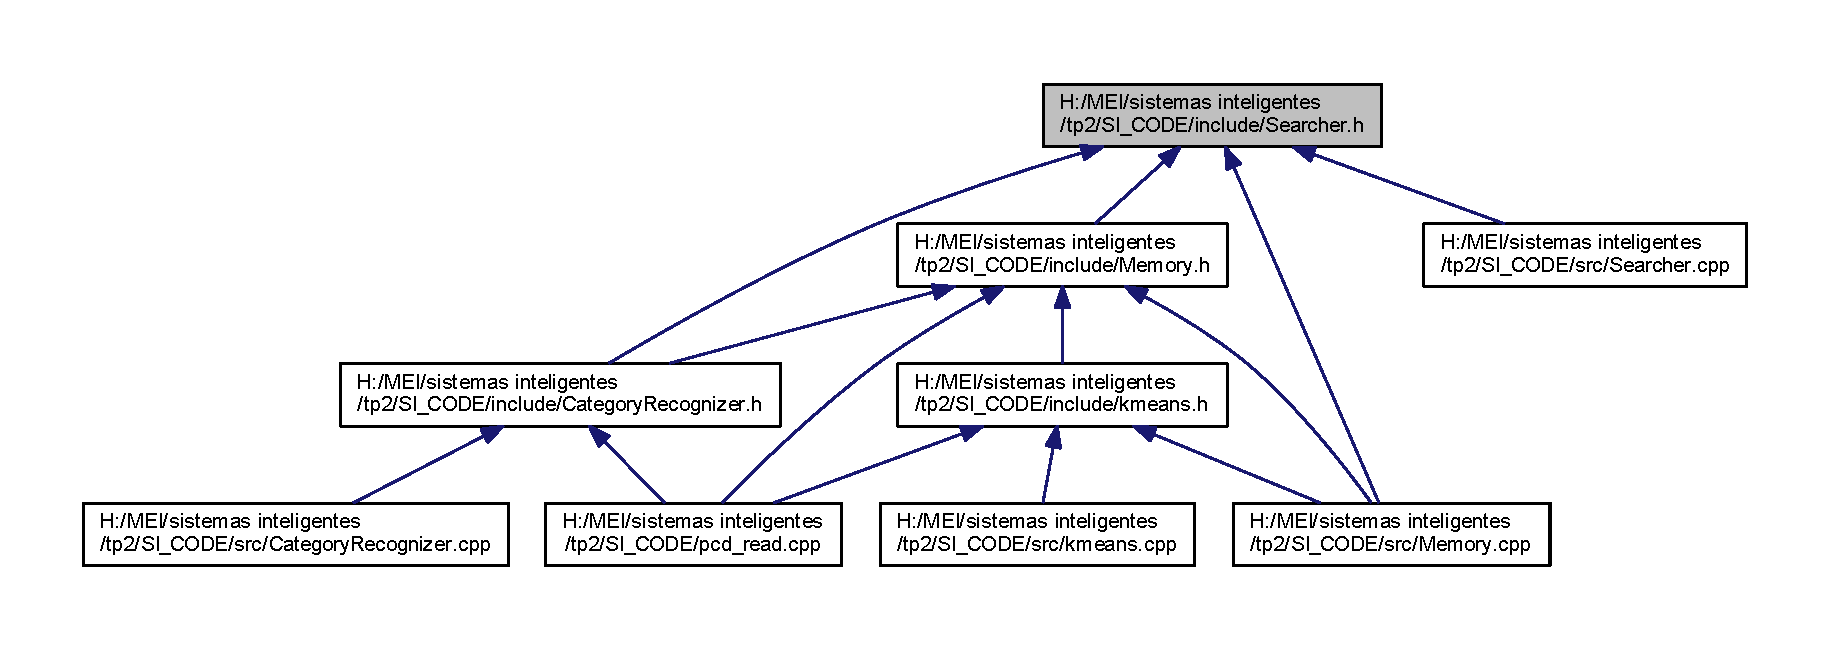
\includegraphics[width=350pt]{_searcher_8h__dep__incl}
\end{center}
\end{figure}
\subsection*{Classes}
\begin{DoxyCompactItemize}
\item 
class \hyperlink{class_searcher}{Searcher}
\begin{DoxyCompactList}\small\item\em A class with functions to search for features in a given search domain. It also provides functions for the calculation of the euclidean distance for vectors. \end{DoxyCompactList}\end{DoxyCompactItemize}

\hypertarget{_seq_generator_8h}{}\section{H\+:/\+M\+E\+I/sistemas inteligentes/tp2/\+S\+I\+\_\+\+C\+O\+D\+E/include/\+Seq\+Generator.h File Reference}
\label{_seq_generator_8h}\index{H\+:/\+M\+E\+I/sistemas inteligentes/tp2/\+S\+I\+\_\+\+C\+O\+D\+E/include/\+Seq\+Generator.\+h@{H\+:/\+M\+E\+I/sistemas inteligentes/tp2/\+S\+I\+\_\+\+C\+O\+D\+E/include/\+Seq\+Generator.\+h}}
This graph shows which files directly or indirectly include this file\+:
\nopagebreak
\begin{figure}[H]
\begin{center}
\leavevmode
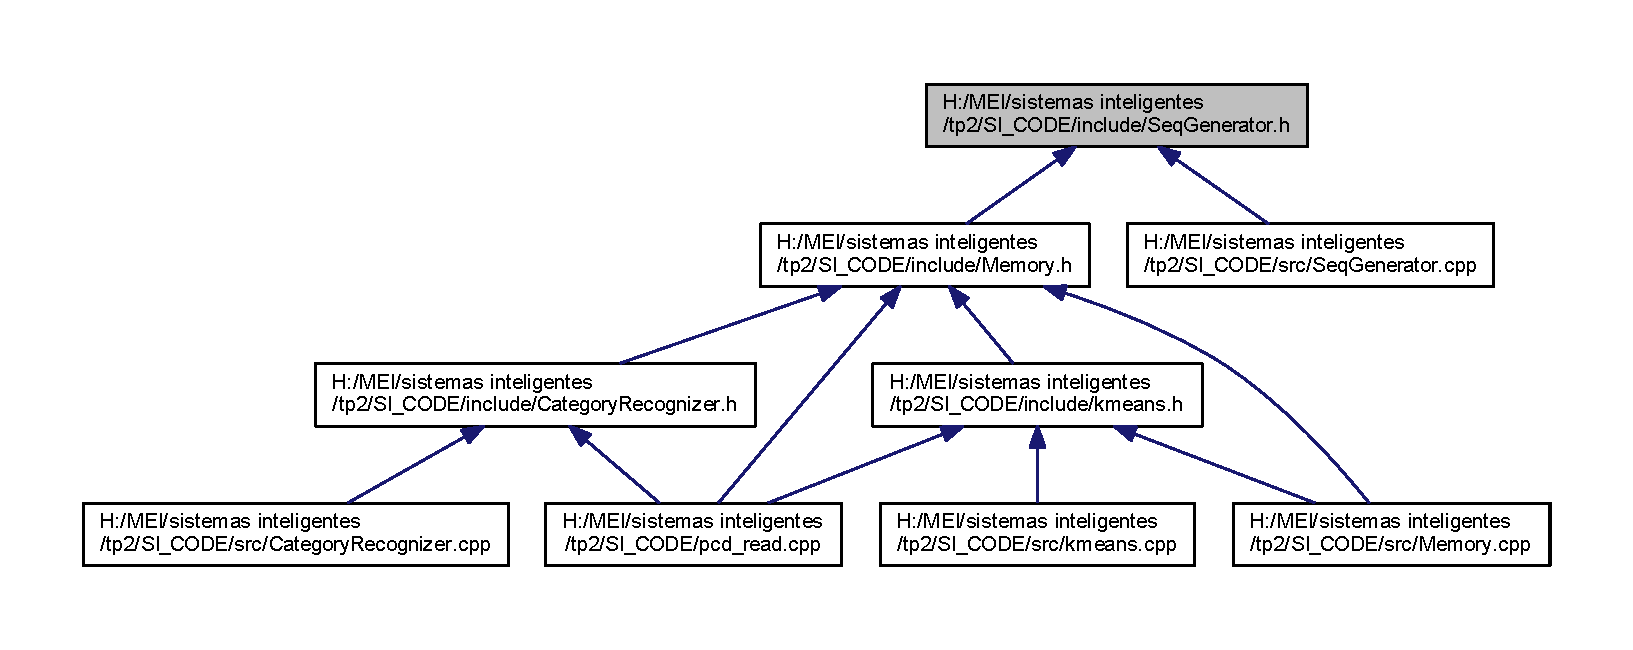
\includegraphics[width=350pt]{_seq_generator_8h__dep__incl}
\end{center}
\end{figure}
\subsection*{Classes}
\begin{DoxyCompactItemize}
\item 
class \hyperlink{class_seq_generator}{Seq\+Generator}
\begin{DoxyCompactList}\small\item\em Uses an int internal variable to generate sequential integer identifiers. \end{DoxyCompactList}\end{DoxyCompactItemize}

\hypertarget{_test_result_8h}{}\section{H\+:/\+M\+E\+I/sistemas inteligentes/tp2/\+S\+I\+\_\+\+C\+O\+D\+E/include/\+Test\+Result.h File Reference}
\label{_test_result_8h}\index{H\+:/\+M\+E\+I/sistemas inteligentes/tp2/\+S\+I\+\_\+\+C\+O\+D\+E/include/\+Test\+Result.\+h@{H\+:/\+M\+E\+I/sistemas inteligentes/tp2/\+S\+I\+\_\+\+C\+O\+D\+E/include/\+Test\+Result.\+h}}
{\ttfamily \#include $<$vector$>$}\newline
{\ttfamily \#include $<$map$>$}\newline
{\ttfamily \#include $<$string$>$}\newline
{\ttfamily \#include \char`\"{}Measure.\+h\char`\"{}}\newline
{\ttfamily \#include \char`\"{}Category.\+h\char`\"{}}\newline
{\ttfamily \#include $<$tr1/unordered\+\_\+map$>$}\newline
Include dependency graph for Test\+Result.\+h\+:
\nopagebreak
\begin{figure}[H]
\begin{center}
\leavevmode
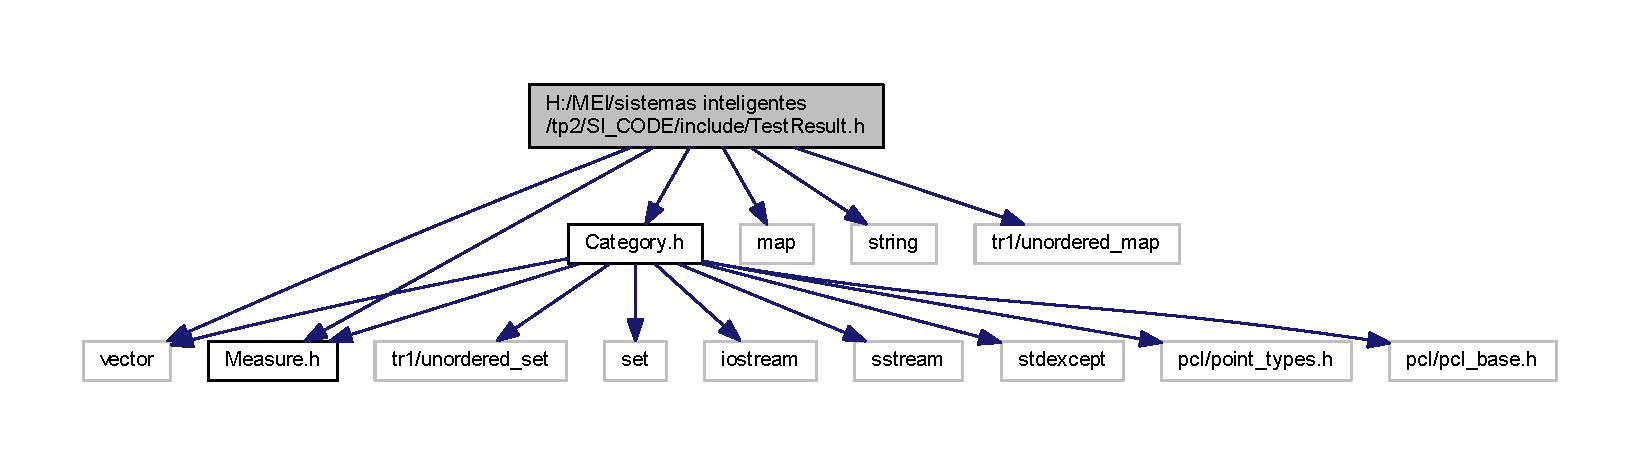
\includegraphics[width=350pt]{_test_result_8h__incl}
\end{center}
\end{figure}
This graph shows which files directly or indirectly include this file\+:
\nopagebreak
\begin{figure}[H]
\begin{center}
\leavevmode
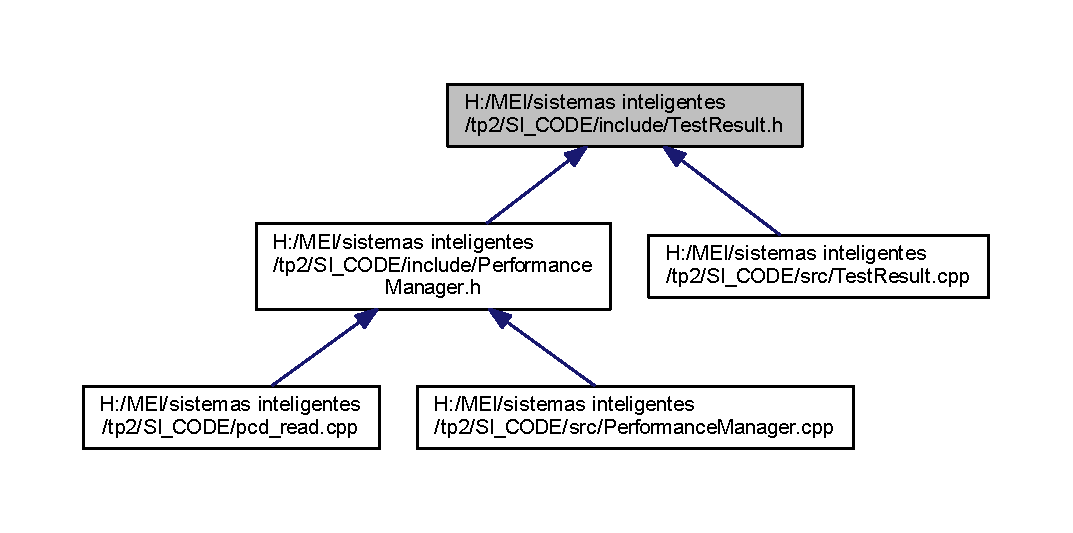
\includegraphics[width=350pt]{_test_result_8h__dep__incl}
\end{center}
\end{figure}
\subsection*{Classes}
\begin{DoxyCompactItemize}
\item 
class \hyperlink{class_test_result}{Test\+Result}
\begin{DoxyCompactList}\small\item\em Holds the performance test results for individual test runs. \end{DoxyCompactList}\end{DoxyCompactItemize}

\hypertarget{_viewer_8h}{}\section{H\+:/\+M\+E\+I/sistemas inteligentes/tp2/\+S\+I\+\_\+\+C\+O\+D\+E/include/\+Viewer.h File Reference}
\label{_viewer_8h}\index{H\+:/\+M\+E\+I/sistemas inteligentes/tp2/\+S\+I\+\_\+\+C\+O\+D\+E/include/\+Viewer.\+h@{H\+:/\+M\+E\+I/sistemas inteligentes/tp2/\+S\+I\+\_\+\+C\+O\+D\+E/include/\+Viewer.\+h}}
{\ttfamily \#include $<$include.\+h$>$}\newline
Include dependency graph for Viewer.\+h\+:
\nopagebreak
\begin{figure}[H]
\begin{center}
\leavevmode
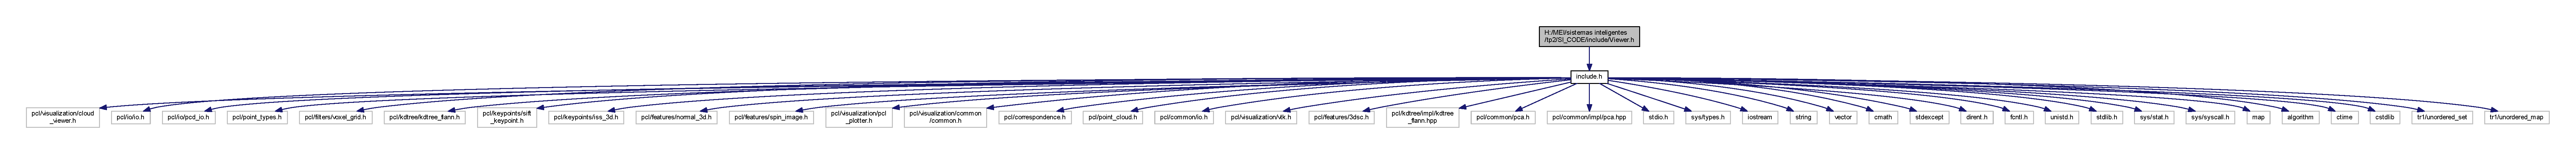
\includegraphics[width=350pt]{_viewer_8h__incl}
\end{center}
\end{figure}
This graph shows which files directly or indirectly include this file\+:
\nopagebreak
\begin{figure}[H]
\begin{center}
\leavevmode
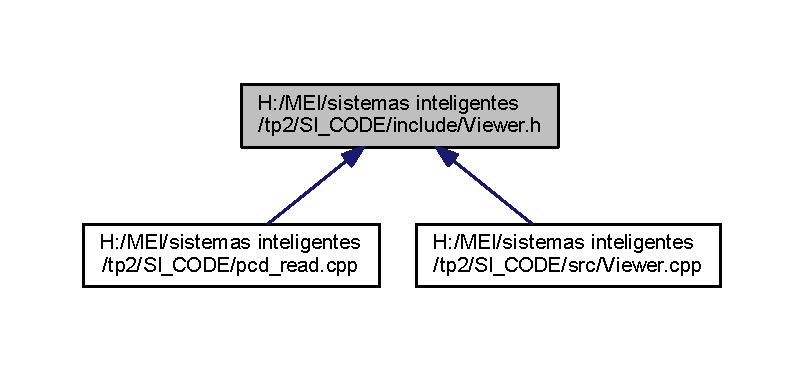
\includegraphics[width=350pt]{_viewer_8h__dep__incl}
\end{center}
\end{figure}
\subsection*{Classes}
\begin{DoxyCompactItemize}
\item 
class \hyperlink{class_viewer}{Viewer}
\begin{DoxyCompactList}\small\item\em Functions for visualization of points$\vert$features and histograms. \end{DoxyCompactList}\end{DoxyCompactItemize}

\hypertarget{_wss_bag_8h}{}\section{H\+:/\+M\+E\+I/sistemas inteligentes/tp2/\+S\+I\+\_\+\+C\+O\+D\+E/include/\+Wss\+Bag.h File Reference}
\label{_wss_bag_8h}\index{H\+:/\+M\+E\+I/sistemas inteligentes/tp2/\+S\+I\+\_\+\+C\+O\+D\+E/include/\+Wss\+Bag.\+h@{H\+:/\+M\+E\+I/sistemas inteligentes/tp2/\+S\+I\+\_\+\+C\+O\+D\+E/include/\+Wss\+Bag.\+h}}
{\ttfamily \#include $<$math.\+h$>$}\newline
Include dependency graph for Wss\+Bag.\+h\+:
\nopagebreak
\begin{figure}[H]
\begin{center}
\leavevmode
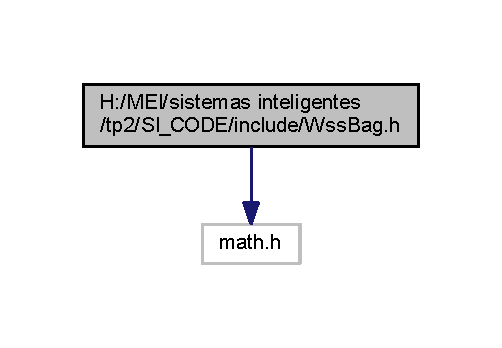
\includegraphics[width=241pt]{_wss_bag_8h__incl}
\end{center}
\end{figure}
This graph shows which files directly or indirectly include this file\+:
\nopagebreak
\begin{figure}[H]
\begin{center}
\leavevmode
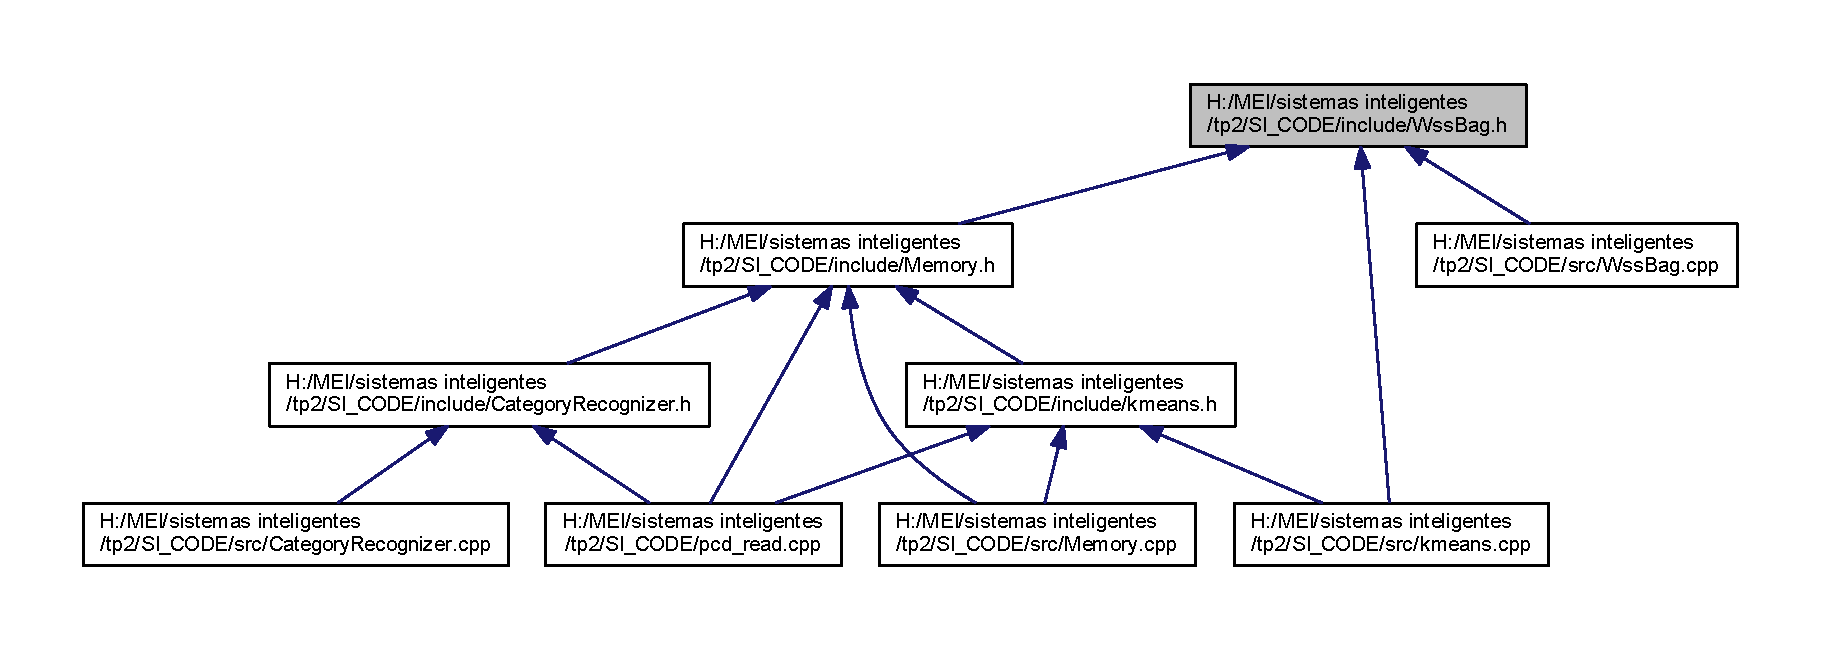
\includegraphics[width=350pt]{_wss_bag_8h__dep__incl}
\end{center}
\end{figure}
\subsection*{Classes}
\begin{DoxyCompactItemize}
\item 
class \hyperlink{class_wss_bag}{Wss\+Bag}
\begin{DoxyCompactList}\small\item\em Utility class to hold numeric values. \end{DoxyCompactList}\end{DoxyCompactItemize}

\hypertarget{pcd__read_8cpp}{}\section{H\+:/\+M\+E\+I/sistemas inteligentes/tp2/\+S\+I\+\_\+\+C\+O\+D\+E/pcd\+\_\+read.cpp File Reference}
\label{pcd__read_8cpp}\index{H\+:/\+M\+E\+I/sistemas inteligentes/tp2/\+S\+I\+\_\+\+C\+O\+D\+E/pcd\+\_\+read.\+cpp@{H\+:/\+M\+E\+I/sistemas inteligentes/tp2/\+S\+I\+\_\+\+C\+O\+D\+E/pcd\+\_\+read.\+cpp}}
{\ttfamily \#include $<$iostream$>$}\newline
{\ttfamily \#include $<$vector$>$}\newline
{\ttfamily \#include $<$map$>$}\newline
{\ttfamily \#include $<$sstream$>$}\newline
{\ttfamily \#include $<$stdlib.\+h$>$}\newline
{\ttfamily \#include $<$algorithm$>$}\newline
{\ttfamily \#include $<$functional$>$}\newline
{\ttfamily \#include $<$iomanip$>$}\newline
{\ttfamily \#include $<$fstream$>$}\newline
{\ttfamily \#include $<$pcl/io/pcd\+\_\+io.\+h$>$}\newline
{\ttfamily \#include $<$pcl/point\+\_\+types.\+h$>$}\newline
{\ttfamily \#include $<$pcl/filters/voxel\+\_\+grid.\+h$>$}\newline
{\ttfamily \#include $<$pcl/features/normal\+\_\+3d.\+h$>$}\newline
{\ttfamily \#include $<$pcl/features/spin\+\_\+image.\+h$>$}\newline
{\ttfamily \#include $<$pcl/pcl\+\_\+base.\+h$>$}\newline
{\ttfamily \#include $<$include.\+h$>$}\newline
{\ttfamily \#include $<$Viewer.\+h$>$}\newline
{\ttfamily \#include \char`\"{}kmeans.\+h\char`\"{}}\newline
{\ttfamily \#include \char`\"{}Memory.\+h\char`\"{}}\newline
{\ttfamily \#include \char`\"{}Cluster.\+h\char`\"{}}\newline
{\ttfamily \#include \char`\"{}Performance\+Manager.\+h\char`\"{}}\newline
{\ttfamily \#include $<$Feature\+Extractor.\+h$>$}\newline
{\ttfamily \#include $<$Object\+View\+Repository.\+h$>$}\newline
{\ttfamily \#include $<$Category\+Recognizer.\+h$>$}\newline
{\ttfamily \#include $<$time.\+h$>$}\newline
{\ttfamily \#include $<$math.\+h$>$}\newline
{\ttfamily \#include $<$cstdlib$>$}\newline
{\ttfamily \#include $<$stdio.\+h$>$}\newline
Include dependency graph for pcd\+\_\+read.\+cpp\+:
\nopagebreak
\begin{figure}[H]
\begin{center}
\leavevmode
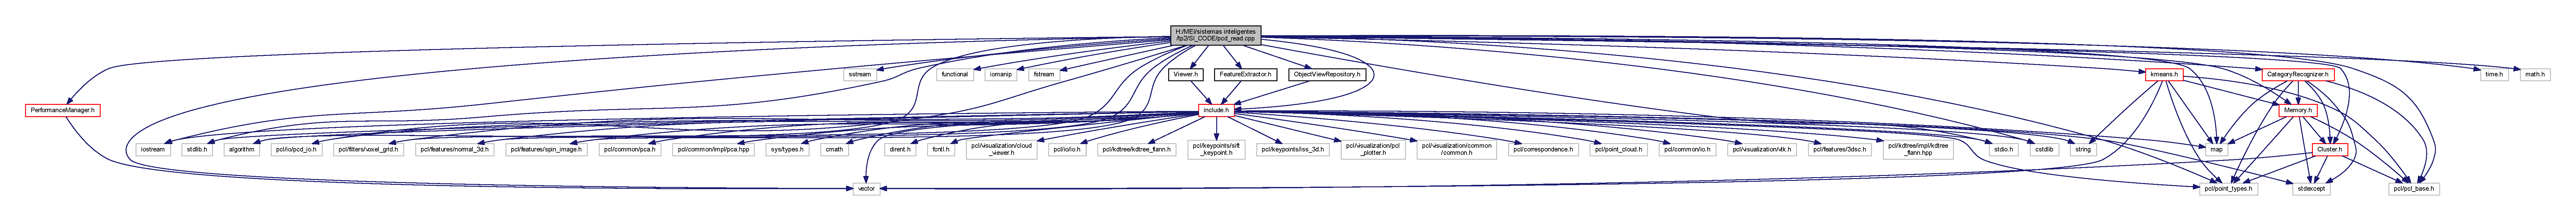
\includegraphics[width=350pt]{pcd__read_8cpp__incl}
\end{center}
\end{figure}
\subsection*{Functions}
\begin{DoxyCompactItemize}
\item 
bool \hyperlink{pcd__read_8cpp_a556b3c6905dcddb8e025f01fe26aeeb0}{load\+\_\+configuration} (const char $\ast$\hyperlink{pcd__read_8cpp_aca091ce0edc2826a2daa09632fe1df87}{configuration\+\_\+file})
\item 
void \hyperlink{pcd__read_8cpp_aa45f069fe76674a03f3dd560dd00b1ee}{print\+Configuration} ()
\item 
char \hyperlink{pcd__read_8cpp_a04b60e3f5695797d1c8a637116847b0d}{run\+Test} (\hyperlink{class_memory}{Memory} \&memory, \hyperlink{class_test_result}{Test\+Result} \&test\+Result)
\item 
int \hyperlink{pcd__read_8cpp_a3c04138a5bfe5d72780bb7e82a18e627}{main} (int argc, char $\ast$$\ast$argv)
\end{DoxyCompactItemize}
\subsection*{Variables}
\begin{DoxyCompactItemize}
\item 
float \hyperlink{pcd__read_8cpp_abb53629fa0b24a5b441a9459a9a260bd}{voxel\+\_\+size} = 0.\+03
\item 
float \hyperlink{pcd__read_8cpp_a138272d8c4416a17717f968a40c689a0}{search\+\_\+radius} = 0.\+1
\item 
int \hyperlink{pcd__read_8cpp_a0e2e740afd510cfe652a1836ffbad209}{window\+\_\+width} = 8
\item 
float \hyperlink{pcd__read_8cpp_abed5c1c3716fc66df9f1a01a430aa8cc}{support\+\_\+lenght} = 0.\+1
\item 
float \hyperlink{pcd__read_8cpp_a13fd0ebf6c809f68d2b0e9bfc16bf68d}{support\+\_\+angle} = 0
\item 
float \hyperlink{pcd__read_8cpp_abbd3dac675fcfc5a5b1d4650518f3771}{min\+\_\+pts\+\_\+neighbours} = 0
\item 
double \hyperlink{pcd__read_8cpp_a509a4ff42b75fb552a368fb612b4d5aa}{feature\+Redundancy\+Treshold}
\item 
float \hyperlink{pcd__read_8cpp_aa84893582aa7db6e7f8d264c9d5f551d}{memory\+Decay\+Factor}
\item 
float \hyperlink{pcd__read_8cpp_a079ca08c1f50cffd8aeed76cb32f953d}{memory\+Decay\+Treshold}
\item 
long long \hyperlink{pcd__read_8cpp_a8d4989d5c738bf1af4de9534934b31c2}{max\+Num\+Features\+In\+Memory}
\item 
float \hyperlink{pcd__read_8cpp_aff7e6408eaf90a97c24e2040a8276c9d}{redistribute\+\_\+g\+Weights\+\_\+search\+\_\+radius} = 0.\+05
\item 
bool \hyperlink{pcd__read_8cpp_a117352cc494cc62c6b2f1882786a332c}{D\+E\+B\+UG} = false
\item 
const char $\ast$ \hyperlink{pcd__read_8cpp_acd0fefcf1eadbf91d3e55e688fdfed78}{object\+\_\+views\+\_\+directory} = N\+U\+LL
\item 
int \hyperlink{pcd__read_8cpp_a21d538faa7b6b1c86f9d819afb80545a}{n\+Categories} = 0
\item 
float \hyperlink{pcd__read_8cpp_ac20bcaf1ef4dcd80403aa6226205f078}{training\+Percentage} = 0.\+0
\item 
int \hyperlink{pcd__read_8cpp_ae4d2a6bfe8a5f3769966bedeb51fd5ce}{number\+Of\+Tests} = 0
\item 
const char $\ast$ \hyperlink{pcd__read_8cpp_aca091ce0edc2826a2daa09632fe1df87}{configuration\+\_\+file} = N\+U\+LL
\item 
bool \hyperlink{pcd__read_8cpp_a9b88421536cf9e112537307343ce61ab}{forget} = false
\item 
int \hyperlink{pcd__read_8cpp_ad7293039828c875da50e40a0640f3dfa}{n\+Views\+To\+See\+Per\+Category} = 0
\item 
bool \hyperlink{pcd__read_8cpp_a70b060316aa5f0bcce50bae018f006f2}{rand\+Shuffle} = false
\end{DoxyCompactItemize}


\subsection{Function Documentation}
\mbox{\Hypertarget{pcd__read_8cpp_a556b3c6905dcddb8e025f01fe26aeeb0}\label{pcd__read_8cpp_a556b3c6905dcddb8e025f01fe26aeeb0}} 
\index{pcd\+\_\+read.\+cpp@{pcd\+\_\+read.\+cpp}!load\+\_\+configuration@{load\+\_\+configuration}}
\index{load\+\_\+configuration@{load\+\_\+configuration}!pcd\+\_\+read.\+cpp@{pcd\+\_\+read.\+cpp}}
\subsubsection{\texorpdfstring{load\+\_\+configuration()}{load\_configuration()}}
{\footnotesize\ttfamily bool load\+\_\+configuration (\begin{DoxyParamCaption}\item[{const char $\ast$}]{configuration\+\_\+file }\end{DoxyParamCaption})}

Loads the configuration file from disk. 

Definition at line 74 of file pcd\+\_\+read.\+cpp.

\mbox{\Hypertarget{pcd__read_8cpp_a3c04138a5bfe5d72780bb7e82a18e627}\label{pcd__read_8cpp_a3c04138a5bfe5d72780bb7e82a18e627}} 
\index{pcd\+\_\+read.\+cpp@{pcd\+\_\+read.\+cpp}!main@{main}}
\index{main@{main}!pcd\+\_\+read.\+cpp@{pcd\+\_\+read.\+cpp}}
\subsubsection{\texorpdfstring{main()}{main()}}
{\footnotesize\ttfamily int main (\begin{DoxyParamCaption}\item[{int}]{argc,  }\item[{char $\ast$$\ast$}]{argv }\end{DoxyParamCaption})}

The application entry point. 

Definition at line 358 of file pcd\+\_\+read.\+cpp.

\mbox{\Hypertarget{pcd__read_8cpp_aa45f069fe76674a03f3dd560dd00b1ee}\label{pcd__read_8cpp_aa45f069fe76674a03f3dd560dd00b1ee}} 
\index{pcd\+\_\+read.\+cpp@{pcd\+\_\+read.\+cpp}!print\+Configuration@{print\+Configuration}}
\index{print\+Configuration@{print\+Configuration}!pcd\+\_\+read.\+cpp@{pcd\+\_\+read.\+cpp}}
\subsubsection{\texorpdfstring{print\+Configuration()}{printConfiguration()}}
{\footnotesize\ttfamily void print\+Configuration (\begin{DoxyParamCaption}{ }\end{DoxyParamCaption})}

Prints the application configuration. 

Definition at line 124 of file pcd\+\_\+read.\+cpp.

\mbox{\Hypertarget{pcd__read_8cpp_a04b60e3f5695797d1c8a637116847b0d}\label{pcd__read_8cpp_a04b60e3f5695797d1c8a637116847b0d}} 
\index{pcd\+\_\+read.\+cpp@{pcd\+\_\+read.\+cpp}!run\+Test@{run\+Test}}
\index{run\+Test@{run\+Test}!pcd\+\_\+read.\+cpp@{pcd\+\_\+read.\+cpp}}
\subsubsection{\texorpdfstring{run\+Test()}{runTest()}}
{\footnotesize\ttfamily char run\+Test (\begin{DoxyParamCaption}\item[{\hyperlink{class_memory}{Memory} \&}]{memory,  }\item[{\hyperlink{class_test_result}{Test\+Result} \&}]{test\+Result }\end{DoxyParamCaption})}

Runs a test. A test includes 2 phases\+: trainig and learning. 

Definition at line 161 of file pcd\+\_\+read.\+cpp.



\subsection{Variable Documentation}
\mbox{\Hypertarget{pcd__read_8cpp_aca091ce0edc2826a2daa09632fe1df87}\label{pcd__read_8cpp_aca091ce0edc2826a2daa09632fe1df87}} 
\index{pcd\+\_\+read.\+cpp@{pcd\+\_\+read.\+cpp}!configuration\+\_\+file@{configuration\+\_\+file}}
\index{configuration\+\_\+file@{configuration\+\_\+file}!pcd\+\_\+read.\+cpp@{pcd\+\_\+read.\+cpp}}
\subsubsection{\texorpdfstring{configuration\+\_\+file}{configuration\_file}}
{\footnotesize\ttfamily const char$\ast$ configuration\+\_\+file = N\+U\+LL}



Definition at line 64 of file pcd\+\_\+read.\+cpp.

\mbox{\Hypertarget{pcd__read_8cpp_a117352cc494cc62c6b2f1882786a332c}\label{pcd__read_8cpp_a117352cc494cc62c6b2f1882786a332c}} 
\index{pcd\+\_\+read.\+cpp@{pcd\+\_\+read.\+cpp}!D\+E\+B\+UG@{D\+E\+B\+UG}}
\index{D\+E\+B\+UG@{D\+E\+B\+UG}!pcd\+\_\+read.\+cpp@{pcd\+\_\+read.\+cpp}}
\subsubsection{\texorpdfstring{D\+E\+B\+UG}{DEBUG}}
{\footnotesize\ttfamily bool D\+E\+B\+UG = false}



Definition at line 58 of file pcd\+\_\+read.\+cpp.

\mbox{\Hypertarget{pcd__read_8cpp_a509a4ff42b75fb552a368fb612b4d5aa}\label{pcd__read_8cpp_a509a4ff42b75fb552a368fb612b4d5aa}} 
\index{pcd\+\_\+read.\+cpp@{pcd\+\_\+read.\+cpp}!feature\+Redundancy\+Treshold@{feature\+Redundancy\+Treshold}}
\index{feature\+Redundancy\+Treshold@{feature\+Redundancy\+Treshold}!pcd\+\_\+read.\+cpp@{pcd\+\_\+read.\+cpp}}
\subsubsection{\texorpdfstring{feature\+Redundancy\+Treshold}{featureRedundancyTreshold}}
{\footnotesize\ttfamily double feature\+Redundancy\+Treshold}



Definition at line 51 of file pcd\+\_\+read.\+cpp.

\mbox{\Hypertarget{pcd__read_8cpp_a9b88421536cf9e112537307343ce61ab}\label{pcd__read_8cpp_a9b88421536cf9e112537307343ce61ab}} 
\index{pcd\+\_\+read.\+cpp@{pcd\+\_\+read.\+cpp}!forget@{forget}}
\index{forget@{forget}!pcd\+\_\+read.\+cpp@{pcd\+\_\+read.\+cpp}}
\subsubsection{\texorpdfstring{forget}{forget}}
{\footnotesize\ttfamily bool forget = false}



Definition at line 65 of file pcd\+\_\+read.\+cpp.

\mbox{\Hypertarget{pcd__read_8cpp_a8d4989d5c738bf1af4de9534934b31c2}\label{pcd__read_8cpp_a8d4989d5c738bf1af4de9534934b31c2}} 
\index{pcd\+\_\+read.\+cpp@{pcd\+\_\+read.\+cpp}!max\+Num\+Features\+In\+Memory@{max\+Num\+Features\+In\+Memory}}
\index{max\+Num\+Features\+In\+Memory@{max\+Num\+Features\+In\+Memory}!pcd\+\_\+read.\+cpp@{pcd\+\_\+read.\+cpp}}
\subsubsection{\texorpdfstring{max\+Num\+Features\+In\+Memory}{maxNumFeaturesInMemory}}
{\footnotesize\ttfamily long long max\+Num\+Features\+In\+Memory}



Definition at line 54 of file pcd\+\_\+read.\+cpp.

\mbox{\Hypertarget{pcd__read_8cpp_aa84893582aa7db6e7f8d264c9d5f551d}\label{pcd__read_8cpp_aa84893582aa7db6e7f8d264c9d5f551d}} 
\index{pcd\+\_\+read.\+cpp@{pcd\+\_\+read.\+cpp}!memory\+Decay\+Factor@{memory\+Decay\+Factor}}
\index{memory\+Decay\+Factor@{memory\+Decay\+Factor}!pcd\+\_\+read.\+cpp@{pcd\+\_\+read.\+cpp}}
\subsubsection{\texorpdfstring{memory\+Decay\+Factor}{memoryDecayFactor}}
{\footnotesize\ttfamily float memory\+Decay\+Factor}



Definition at line 52 of file pcd\+\_\+read.\+cpp.

\mbox{\Hypertarget{pcd__read_8cpp_a079ca08c1f50cffd8aeed76cb32f953d}\label{pcd__read_8cpp_a079ca08c1f50cffd8aeed76cb32f953d}} 
\index{pcd\+\_\+read.\+cpp@{pcd\+\_\+read.\+cpp}!memory\+Decay\+Treshold@{memory\+Decay\+Treshold}}
\index{memory\+Decay\+Treshold@{memory\+Decay\+Treshold}!pcd\+\_\+read.\+cpp@{pcd\+\_\+read.\+cpp}}
\subsubsection{\texorpdfstring{memory\+Decay\+Treshold}{memoryDecayTreshold}}
{\footnotesize\ttfamily float memory\+Decay\+Treshold}



Definition at line 53 of file pcd\+\_\+read.\+cpp.

\mbox{\Hypertarget{pcd__read_8cpp_abbd3dac675fcfc5a5b1d4650518f3771}\label{pcd__read_8cpp_abbd3dac675fcfc5a5b1d4650518f3771}} 
\index{pcd\+\_\+read.\+cpp@{pcd\+\_\+read.\+cpp}!min\+\_\+pts\+\_\+neighbours@{min\+\_\+pts\+\_\+neighbours}}
\index{min\+\_\+pts\+\_\+neighbours@{min\+\_\+pts\+\_\+neighbours}!pcd\+\_\+read.\+cpp@{pcd\+\_\+read.\+cpp}}
\subsubsection{\texorpdfstring{min\+\_\+pts\+\_\+neighbours}{min\_pts\_neighbours}}
{\footnotesize\ttfamily float min\+\_\+pts\+\_\+neighbours = 0}



Definition at line 49 of file pcd\+\_\+read.\+cpp.

\mbox{\Hypertarget{pcd__read_8cpp_a21d538faa7b6b1c86f9d819afb80545a}\label{pcd__read_8cpp_a21d538faa7b6b1c86f9d819afb80545a}} 
\index{pcd\+\_\+read.\+cpp@{pcd\+\_\+read.\+cpp}!n\+Categories@{n\+Categories}}
\index{n\+Categories@{n\+Categories}!pcd\+\_\+read.\+cpp@{pcd\+\_\+read.\+cpp}}
\subsubsection{\texorpdfstring{n\+Categories}{nCategories}}
{\footnotesize\ttfamily int n\+Categories = 0}



Definition at line 61 of file pcd\+\_\+read.\+cpp.

\mbox{\Hypertarget{pcd__read_8cpp_ae4d2a6bfe8a5f3769966bedeb51fd5ce}\label{pcd__read_8cpp_ae4d2a6bfe8a5f3769966bedeb51fd5ce}} 
\index{pcd\+\_\+read.\+cpp@{pcd\+\_\+read.\+cpp}!number\+Of\+Tests@{number\+Of\+Tests}}
\index{number\+Of\+Tests@{number\+Of\+Tests}!pcd\+\_\+read.\+cpp@{pcd\+\_\+read.\+cpp}}
\subsubsection{\texorpdfstring{number\+Of\+Tests}{numberOfTests}}
{\footnotesize\ttfamily int number\+Of\+Tests = 0}



Definition at line 63 of file pcd\+\_\+read.\+cpp.

\mbox{\Hypertarget{pcd__read_8cpp_ad7293039828c875da50e40a0640f3dfa}\label{pcd__read_8cpp_ad7293039828c875da50e40a0640f3dfa}} 
\index{pcd\+\_\+read.\+cpp@{pcd\+\_\+read.\+cpp}!n\+Views\+To\+See\+Per\+Category@{n\+Views\+To\+See\+Per\+Category}}
\index{n\+Views\+To\+See\+Per\+Category@{n\+Views\+To\+See\+Per\+Category}!pcd\+\_\+read.\+cpp@{pcd\+\_\+read.\+cpp}}
\subsubsection{\texorpdfstring{n\+Views\+To\+See\+Per\+Category}{nViewsToSeePerCategory}}
{\footnotesize\ttfamily int n\+Views\+To\+See\+Per\+Category = 0}



Definition at line 66 of file pcd\+\_\+read.\+cpp.

\mbox{\Hypertarget{pcd__read_8cpp_acd0fefcf1eadbf91d3e55e688fdfed78}\label{pcd__read_8cpp_acd0fefcf1eadbf91d3e55e688fdfed78}} 
\index{pcd\+\_\+read.\+cpp@{pcd\+\_\+read.\+cpp}!object\+\_\+views\+\_\+directory@{object\+\_\+views\+\_\+directory}}
\index{object\+\_\+views\+\_\+directory@{object\+\_\+views\+\_\+directory}!pcd\+\_\+read.\+cpp@{pcd\+\_\+read.\+cpp}}
\subsubsection{\texorpdfstring{object\+\_\+views\+\_\+directory}{object\_views\_directory}}
{\footnotesize\ttfamily const char$\ast$ object\+\_\+views\+\_\+directory = N\+U\+LL}



Definition at line 60 of file pcd\+\_\+read.\+cpp.

\mbox{\Hypertarget{pcd__read_8cpp_a70b060316aa5f0bcce50bae018f006f2}\label{pcd__read_8cpp_a70b060316aa5f0bcce50bae018f006f2}} 
\index{pcd\+\_\+read.\+cpp@{pcd\+\_\+read.\+cpp}!rand\+Shuffle@{rand\+Shuffle}}
\index{rand\+Shuffle@{rand\+Shuffle}!pcd\+\_\+read.\+cpp@{pcd\+\_\+read.\+cpp}}
\subsubsection{\texorpdfstring{rand\+Shuffle}{randShuffle}}
{\footnotesize\ttfamily bool rand\+Shuffle = false}



Definition at line 67 of file pcd\+\_\+read.\+cpp.

\mbox{\Hypertarget{pcd__read_8cpp_aff7e6408eaf90a97c24e2040a8276c9d}\label{pcd__read_8cpp_aff7e6408eaf90a97c24e2040a8276c9d}} 
\index{pcd\+\_\+read.\+cpp@{pcd\+\_\+read.\+cpp}!redistribute\+\_\+g\+Weights\+\_\+search\+\_\+radius@{redistribute\+\_\+g\+Weights\+\_\+search\+\_\+radius}}
\index{redistribute\+\_\+g\+Weights\+\_\+search\+\_\+radius@{redistribute\+\_\+g\+Weights\+\_\+search\+\_\+radius}!pcd\+\_\+read.\+cpp@{pcd\+\_\+read.\+cpp}}
\subsubsection{\texorpdfstring{redistribute\+\_\+g\+Weights\+\_\+search\+\_\+radius}{redistribute\_gWeights\_search\_radius}}
{\footnotesize\ttfamily float redistribute\+\_\+g\+Weights\+\_\+search\+\_\+radius = 0.\+05}



Definition at line 56 of file pcd\+\_\+read.\+cpp.

\mbox{\Hypertarget{pcd__read_8cpp_a138272d8c4416a17717f968a40c689a0}\label{pcd__read_8cpp_a138272d8c4416a17717f968a40c689a0}} 
\index{pcd\+\_\+read.\+cpp@{pcd\+\_\+read.\+cpp}!search\+\_\+radius@{search\+\_\+radius}}
\index{search\+\_\+radius@{search\+\_\+radius}!pcd\+\_\+read.\+cpp@{pcd\+\_\+read.\+cpp}}
\subsubsection{\texorpdfstring{search\+\_\+radius}{search\_radius}}
{\footnotesize\ttfamily float search\+\_\+radius = 0.\+1}



Definition at line 45 of file pcd\+\_\+read.\+cpp.

\mbox{\Hypertarget{pcd__read_8cpp_a13fd0ebf6c809f68d2b0e9bfc16bf68d}\label{pcd__read_8cpp_a13fd0ebf6c809f68d2b0e9bfc16bf68d}} 
\index{pcd\+\_\+read.\+cpp@{pcd\+\_\+read.\+cpp}!support\+\_\+angle@{support\+\_\+angle}}
\index{support\+\_\+angle@{support\+\_\+angle}!pcd\+\_\+read.\+cpp@{pcd\+\_\+read.\+cpp}}
\subsubsection{\texorpdfstring{support\+\_\+angle}{support\_angle}}
{\footnotesize\ttfamily float support\+\_\+angle = 0}



Definition at line 48 of file pcd\+\_\+read.\+cpp.

\mbox{\Hypertarget{pcd__read_8cpp_abed5c1c3716fc66df9f1a01a430aa8cc}\label{pcd__read_8cpp_abed5c1c3716fc66df9f1a01a430aa8cc}} 
\index{pcd\+\_\+read.\+cpp@{pcd\+\_\+read.\+cpp}!support\+\_\+lenght@{support\+\_\+lenght}}
\index{support\+\_\+lenght@{support\+\_\+lenght}!pcd\+\_\+read.\+cpp@{pcd\+\_\+read.\+cpp}}
\subsubsection{\texorpdfstring{support\+\_\+lenght}{support\_lenght}}
{\footnotesize\ttfamily float support\+\_\+lenght = 0.\+1}



Definition at line 47 of file pcd\+\_\+read.\+cpp.

\mbox{\Hypertarget{pcd__read_8cpp_ac20bcaf1ef4dcd80403aa6226205f078}\label{pcd__read_8cpp_ac20bcaf1ef4dcd80403aa6226205f078}} 
\index{pcd\+\_\+read.\+cpp@{pcd\+\_\+read.\+cpp}!training\+Percentage@{training\+Percentage}}
\index{training\+Percentage@{training\+Percentage}!pcd\+\_\+read.\+cpp@{pcd\+\_\+read.\+cpp}}
\subsubsection{\texorpdfstring{training\+Percentage}{trainingPercentage}}
{\footnotesize\ttfamily float training\+Percentage = 0.\+0}



Definition at line 62 of file pcd\+\_\+read.\+cpp.

\mbox{\Hypertarget{pcd__read_8cpp_abb53629fa0b24a5b441a9459a9a260bd}\label{pcd__read_8cpp_abb53629fa0b24a5b441a9459a9a260bd}} 
\index{pcd\+\_\+read.\+cpp@{pcd\+\_\+read.\+cpp}!voxel\+\_\+size@{voxel\+\_\+size}}
\index{voxel\+\_\+size@{voxel\+\_\+size}!pcd\+\_\+read.\+cpp@{pcd\+\_\+read.\+cpp}}
\subsubsection{\texorpdfstring{voxel\+\_\+size}{voxel\_size}}
{\footnotesize\ttfamily float voxel\+\_\+size = 0.\+03}



Definition at line 42 of file pcd\+\_\+read.\+cpp.

\mbox{\Hypertarget{pcd__read_8cpp_a0e2e740afd510cfe652a1836ffbad209}\label{pcd__read_8cpp_a0e2e740afd510cfe652a1836ffbad209}} 
\index{pcd\+\_\+read.\+cpp@{pcd\+\_\+read.\+cpp}!window\+\_\+width@{window\+\_\+width}}
\index{window\+\_\+width@{window\+\_\+width}!pcd\+\_\+read.\+cpp@{pcd\+\_\+read.\+cpp}}
\subsubsection{\texorpdfstring{window\+\_\+width}{window\_width}}
{\footnotesize\ttfamily int window\+\_\+width = 8}



Definition at line 46 of file pcd\+\_\+read.\+cpp.


\hypertarget{_bss_bag_8cpp}{}\section{H\+:/\+M\+E\+I/sistemas inteligentes/tp2/\+S\+I\+\_\+\+C\+O\+D\+E/src/\+Bss\+Bag.cpp File Reference}
\label{_bss_bag_8cpp}\index{H\+:/\+M\+E\+I/sistemas inteligentes/tp2/\+S\+I\+\_\+\+C\+O\+D\+E/src/\+Bss\+Bag.\+cpp@{H\+:/\+M\+E\+I/sistemas inteligentes/tp2/\+S\+I\+\_\+\+C\+O\+D\+E/src/\+Bss\+Bag.\+cpp}}
{\ttfamily \#include \char`\"{}Bss\+Bag.\+h\char`\"{}}\newline
Include dependency graph for Bss\+Bag.\+cpp\+:
\nopagebreak
\begin{figure}[H]
\begin{center}
\leavevmode
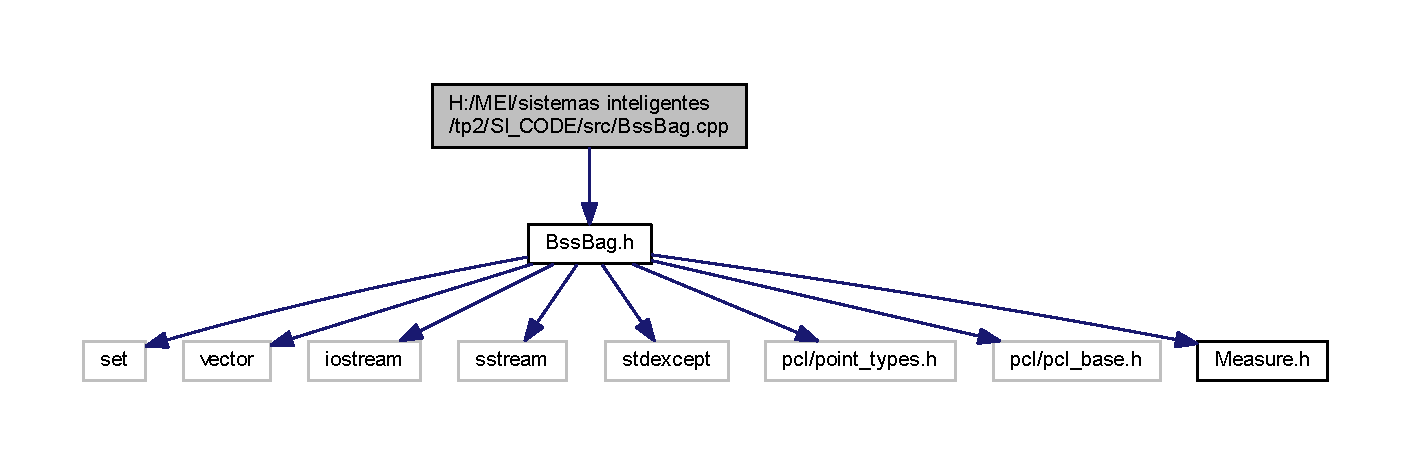
\includegraphics[width=350pt]{_bss_bag_8cpp__incl}
\end{center}
\end{figure}

\hypertarget{_category_8cpp}{}\section{H\+:/\+M\+E\+I/sistemas inteligentes/tp2/\+S\+I\+\_\+\+C\+O\+D\+E/src/\+Category.cpp File Reference}
\label{_category_8cpp}\index{H\+:/\+M\+E\+I/sistemas inteligentes/tp2/\+S\+I\+\_\+\+C\+O\+D\+E/src/\+Category.\+cpp@{H\+:/\+M\+E\+I/sistemas inteligentes/tp2/\+S\+I\+\_\+\+C\+O\+D\+E/src/\+Category.\+cpp}}
{\ttfamily \#include \char`\"{}Category.\+h\char`\"{}}\newline
Include dependency graph for Category.\+cpp\+:
\nopagebreak
\begin{figure}[H]
\begin{center}
\leavevmode
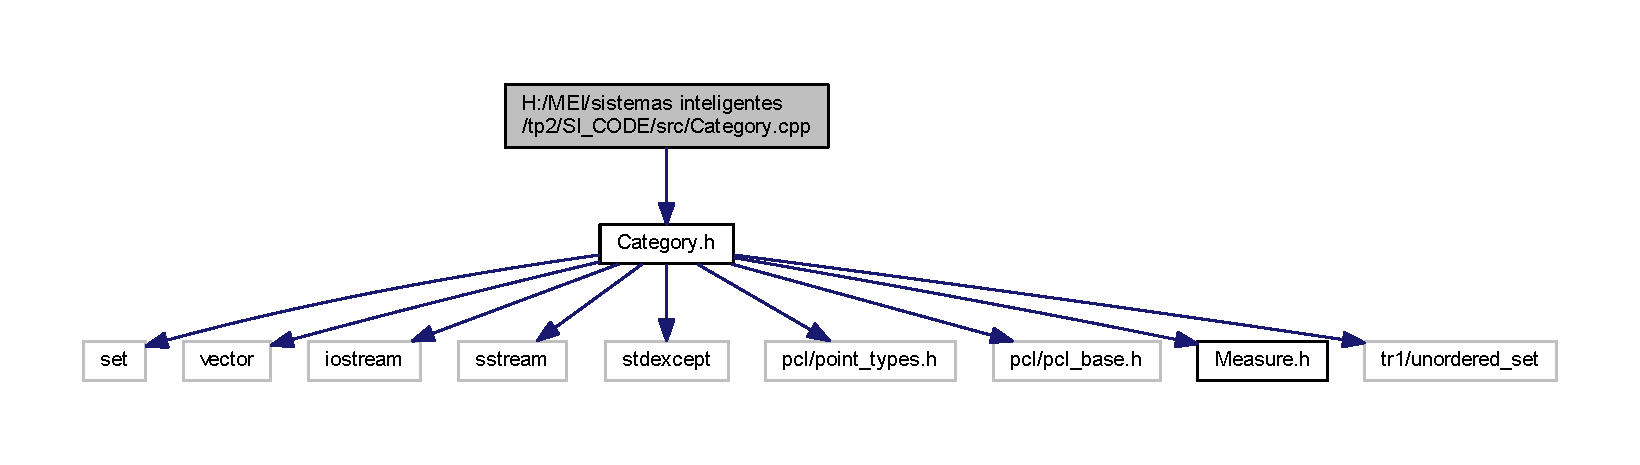
\includegraphics[width=350pt]{_category_8cpp__incl}
\end{center}
\end{figure}

\hypertarget{_category_recognizer_8cpp}{}\section{H\+:/\+M\+E\+I/sistemas inteligentes/tp2/\+S\+I\+\_\+\+C\+O\+D\+E/src/\+Category\+Recognizer.cpp File Reference}
\label{_category_recognizer_8cpp}\index{H\+:/\+M\+E\+I/sistemas inteligentes/tp2/\+S\+I\+\_\+\+C\+O\+D\+E/src/\+Category\+Recognizer.\+cpp@{H\+:/\+M\+E\+I/sistemas inteligentes/tp2/\+S\+I\+\_\+\+C\+O\+D\+E/src/\+Category\+Recognizer.\+cpp}}
{\ttfamily \#include $<$math.\+h$>$}\newline
{\ttfamily \#include $<$algorithm$>$}\newline
{\ttfamily \#include \char`\"{}Category\+Recognizer.\+h\char`\"{}}\newline
Include dependency graph for Category\+Recognizer.\+cpp\+:
\nopagebreak
\begin{figure}[H]
\begin{center}
\leavevmode
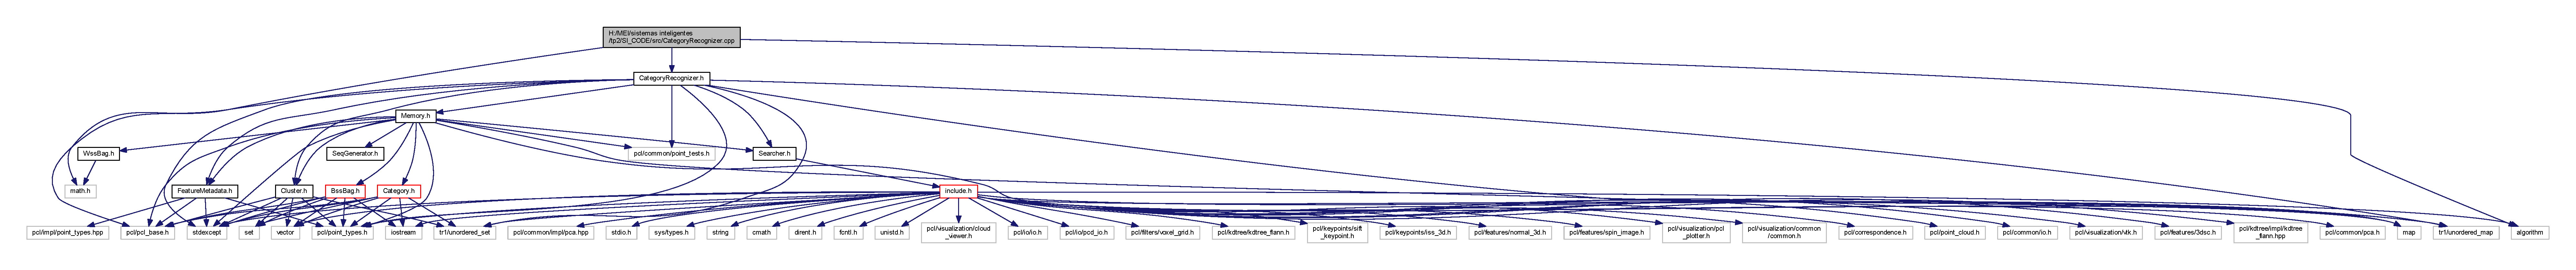
\includegraphics[width=350pt]{_category_recognizer_8cpp__incl}
\end{center}
\end{figure}

\hypertarget{_cluster_8cpp}{}\section{H\+:/\+M\+E\+I/sistemas inteligentes/tp2/\+S\+I\+\_\+\+C\+O\+D\+E/src/\+Cluster.cpp File Reference}
\label{_cluster_8cpp}\index{H\+:/\+M\+E\+I/sistemas inteligentes/tp2/\+S\+I\+\_\+\+C\+O\+D\+E/src/\+Cluster.\+cpp@{H\+:/\+M\+E\+I/sistemas inteligentes/tp2/\+S\+I\+\_\+\+C\+O\+D\+E/src/\+Cluster.\+cpp}}
{\ttfamily \#include $<$stdlib.\+h$>$}\newline
{\ttfamily \#include \char`\"{}Cluster.\+h\char`\"{}}\newline
Include dependency graph for Cluster.\+cpp\+:
\nopagebreak
\begin{figure}[H]
\begin{center}
\leavevmode
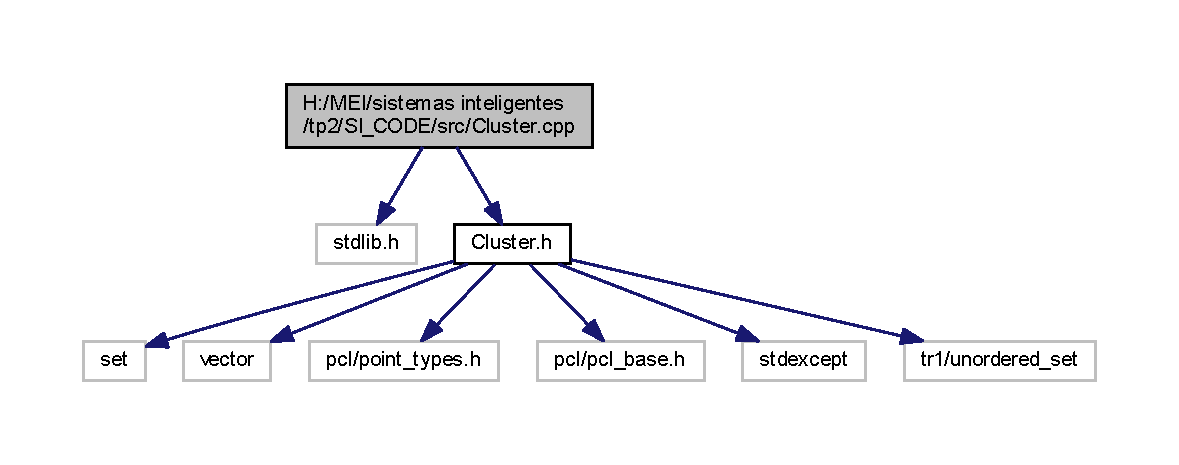
\includegraphics[width=350pt]{_cluster_8cpp__incl}
\end{center}
\end{figure}

\hypertarget{_feature_extractor_8cpp}{}\section{H\+:/\+M\+E\+I/sistemas inteligentes/tp2/\+S\+I\+\_\+\+C\+O\+D\+E/src/\+Feature\+Extractor.cpp File Reference}
\label{_feature_extractor_8cpp}\index{H\+:/\+M\+E\+I/sistemas inteligentes/tp2/\+S\+I\+\_\+\+C\+O\+D\+E/src/\+Feature\+Extractor.\+cpp@{H\+:/\+M\+E\+I/sistemas inteligentes/tp2/\+S\+I\+\_\+\+C\+O\+D\+E/src/\+Feature\+Extractor.\+cpp}}
{\ttfamily \#include $<$Feature\+Extractor.\+h$>$}\newline
Include dependency graph for Feature\+Extractor.\+cpp\+:
\nopagebreak
\begin{figure}[H]
\begin{center}
\leavevmode
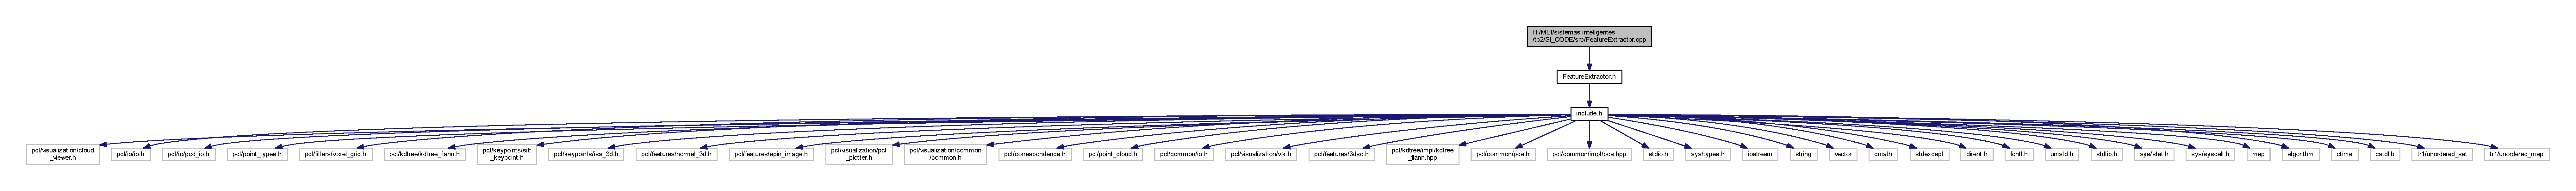
\includegraphics[width=350pt]{_feature_extractor_8cpp__incl}
\end{center}
\end{figure}

\hypertarget{_feature_metadata_8cpp}{}\section{H\+:/\+M\+E\+I/sistemas inteligentes/tp2/\+S\+I\+\_\+\+C\+O\+D\+E/src/\+Feature\+Metadata.cpp File Reference}
\label{_feature_metadata_8cpp}\index{H\+:/\+M\+E\+I/sistemas inteligentes/tp2/\+S\+I\+\_\+\+C\+O\+D\+E/src/\+Feature\+Metadata.\+cpp@{H\+:/\+M\+E\+I/sistemas inteligentes/tp2/\+S\+I\+\_\+\+C\+O\+D\+E/src/\+Feature\+Metadata.\+cpp}}
{\ttfamily \#include \char`\"{}Feature\+Metadata.\+h\char`\"{}}\newline
Include dependency graph for Feature\+Metadata.\+cpp\+:
\nopagebreak
\begin{figure}[H]
\begin{center}
\leavevmode
\includegraphics[width=350pt]{_feature_metadata_8cpp__incl}
\end{center}
\end{figure}

\hypertarget{kmeans_8cpp}{}\section{H\+:/\+M\+E\+I/sistemas inteligentes/tp2/\+S\+I\+\_\+\+C\+O\+D\+E/src/kmeans.cpp File Reference}
\label{kmeans_8cpp}\index{H\+:/\+M\+E\+I/sistemas inteligentes/tp2/\+S\+I\+\_\+\+C\+O\+D\+E/src/kmeans.\+cpp@{H\+:/\+M\+E\+I/sistemas inteligentes/tp2/\+S\+I\+\_\+\+C\+O\+D\+E/src/kmeans.\+cpp}}
{\ttfamily \#include $<$math.\+h$>$}\newline
{\ttfamily \#include $<$limits$>$}\newline
{\ttfamily \#include $<$stdlib.\+h$>$}\newline
{\ttfamily \#include $<$pcl/kdtree/kdtree\+\_\+flann.\+h$>$}\newline
{\ttfamily \#include $<$pcl/kdtree/impl/kdtree\+\_\+flann.\+hpp$>$}\newline
{\ttfamily \#include \char`\"{}kmeans.\+h\char`\"{}}\newline
{\ttfamily \#include \char`\"{}Feature\+Metadata.\+h\char`\"{}}\newline
{\ttfamily \#include \char`\"{}Cluster.\+h\char`\"{}}\newline
{\ttfamily \#include \char`\"{}Default\+Point\+Representation.\+h\char`\"{}}\newline
{\ttfamily \#include \char`\"{}Bss\+Bag.\+h\char`\"{}}\newline
{\ttfamily \#include \char`\"{}Wss\+Bag.\+h\char`\"{}}\newline
{\ttfamily \#include $<$tr1/unordered\+\_\+set$>$}\newline
Include dependency graph for kmeans.\+cpp\+:
\nopagebreak
\begin{figure}[H]
\begin{center}
\leavevmode
\includegraphics[width=350pt]{kmeans_8cpp__incl}
\end{center}
\end{figure}

\hypertarget{_measure_8cpp}{}\section{H\+:/\+M\+E\+I/sistemas inteligentes/tp2/\+S\+I\+\_\+\+C\+O\+D\+E/src/\+Measure.cpp File Reference}
\label{_measure_8cpp}\index{H\+:/\+M\+E\+I/sistemas inteligentes/tp2/\+S\+I\+\_\+\+C\+O\+D\+E/src/\+Measure.\+cpp@{H\+:/\+M\+E\+I/sistemas inteligentes/tp2/\+S\+I\+\_\+\+C\+O\+D\+E/src/\+Measure.\+cpp}}
{\ttfamily \#include \char`\"{}Measure.\+h\char`\"{}}\newline
Include dependency graph for Measure.\+cpp\+:
\nopagebreak
\begin{figure}[H]
\begin{center}
\leavevmode
\includegraphics[width=234pt]{_measure_8cpp__incl}
\end{center}
\end{figure}

\hypertarget{_memory_8cpp}{}\section{H\+:/\+M\+E\+I/sistemas inteligentes/tp2/\+S\+I\+\_\+\+C\+O\+D\+E/src/\+Memory.cpp File Reference}
\label{_memory_8cpp}\index{H\+:/\+M\+E\+I/sistemas inteligentes/tp2/\+S\+I\+\_\+\+C\+O\+D\+E/src/\+Memory.\+cpp@{H\+:/\+M\+E\+I/sistemas inteligentes/tp2/\+S\+I\+\_\+\+C\+O\+D\+E/src/\+Memory.\+cpp}}
{\ttfamily \#include $<$math.\+h$>$}\newline
{\ttfamily \#include $<$algorithm$>$}\newline
{\ttfamily \#include \char`\"{}Memory.\+h\char`\"{}}\newline
{\ttfamily \#include \char`\"{}Searcher.\+h\char`\"{}}\newline
{\ttfamily \#include \char`\"{}kmeans.\+h\char`\"{}}\newline
{\ttfamily \#include $<$tr1/unordered\+\_\+set$>$}\newline
Include dependency graph for Memory.\+cpp\+:
\nopagebreak
\begin{figure}[H]
\begin{center}
\leavevmode
\includegraphics[width=350pt]{_memory_8cpp__incl}
\end{center}
\end{figure}
\subsection*{Classes}
\begin{DoxyCompactItemize}
\item 
class \hyperlink{classpcl_1_1_default_point_representation_3_01_spin_image_01_4}{pcl\+::\+Default\+Point\+Representation$<$ Spin\+Image $>$}
\end{DoxyCompactItemize}
\subsection*{Namespaces}
\begin{DoxyCompactItemize}
\item 
 \hyperlink{namespacepcl}{pcl}
\end{DoxyCompactItemize}

\hypertarget{_object_view_repository_8cpp}{}\section{H\+:/\+M\+E\+I/sistemas inteligentes/tp2/\+S\+I\+\_\+\+C\+O\+D\+E/src/\+Object\+View\+Repository.cpp File Reference}
\label{_object_view_repository_8cpp}\index{H\+:/\+M\+E\+I/sistemas inteligentes/tp2/\+S\+I\+\_\+\+C\+O\+D\+E/src/\+Object\+View\+Repository.\+cpp@{H\+:/\+M\+E\+I/sistemas inteligentes/tp2/\+S\+I\+\_\+\+C\+O\+D\+E/src/\+Object\+View\+Repository.\+cpp}}
{\ttfamily \#include $<$Object\+View\+Repository.\+h$>$}\newline
Include dependency graph for Object\+View\+Repository.\+cpp\+:
\nopagebreak
\begin{figure}[H]
\begin{center}
\leavevmode
\includegraphics[width=350pt]{_object_view_repository_8cpp__incl}
\end{center}
\end{figure}
\subsection*{Functions}
\begin{DoxyCompactItemize}
\item 
int \hyperlink{_object_view_repository_8cpp_acb04e0eba013626be06bd0006a752538}{myrandom} (int i)
\end{DoxyCompactItemize}


\subsection{Function Documentation}
\mbox{\Hypertarget{_object_view_repository_8cpp_acb04e0eba013626be06bd0006a752538}\label{_object_view_repository_8cpp_acb04e0eba013626be06bd0006a752538}} 
\index{Object\+View\+Repository.\+cpp@{Object\+View\+Repository.\+cpp}!myrandom@{myrandom}}
\index{myrandom@{myrandom}!Object\+View\+Repository.\+cpp@{Object\+View\+Repository.\+cpp}}
\subsubsection{\texorpdfstring{myrandom()}{myrandom()}}
{\footnotesize\ttfamily int myrandom (\begin{DoxyParamCaption}\item[{int}]{i }\end{DoxyParamCaption})}



Definition at line 4 of file Object\+View\+Repository.\+cpp.


\hypertarget{_performance_manager_8cpp}{}\section{H\+:/\+M\+E\+I/sistemas inteligentes/tp2/\+S\+I\+\_\+\+C\+O\+D\+E/src/\+Performance\+Manager.cpp File Reference}
\label{_performance_manager_8cpp}\index{H\+:/\+M\+E\+I/sistemas inteligentes/tp2/\+S\+I\+\_\+\+C\+O\+D\+E/src/\+Performance\+Manager.\+cpp@{H\+:/\+M\+E\+I/sistemas inteligentes/tp2/\+S\+I\+\_\+\+C\+O\+D\+E/src/\+Performance\+Manager.\+cpp}}
{\ttfamily \#include \char`\"{}Performance\+Manager.\+h\char`\"{}}\newline
{\ttfamily \#include $<$iomanip$>$}\newline
Include dependency graph for Performance\+Manager.\+cpp\+:
\nopagebreak
\begin{figure}[H]
\begin{center}
\leavevmode
\includegraphics[width=350pt]{_performance_manager_8cpp__incl}
\end{center}
\end{figure}

\hypertarget{_searcher_8cpp}{}\section{H\+:/\+M\+E\+I/sistemas inteligentes/tp2/\+S\+I\+\_\+\+C\+O\+D\+E/src/\+Searcher.cpp File Reference}
\label{_searcher_8cpp}\index{H\+:/\+M\+E\+I/sistemas inteligentes/tp2/\+S\+I\+\_\+\+C\+O\+D\+E/src/\+Searcher.\+cpp@{H\+:/\+M\+E\+I/sistemas inteligentes/tp2/\+S\+I\+\_\+\+C\+O\+D\+E/src/\+Searcher.\+cpp}}
{\ttfamily \#include $<$Searcher.\+h$>$}\newline
Include dependency graph for Searcher.\+cpp\+:
\nopagebreak
\begin{figure}[H]
\begin{center}
\leavevmode
\includegraphics[width=350pt]{_searcher_8cpp__incl}
\end{center}
\end{figure}
\subsection*{Classes}
\begin{DoxyCompactItemize}
\item 
class \hyperlink{classpcl_1_1_default_point_representation_3_01_spin_image_01_4}{pcl\+::\+Default\+Point\+Representation$<$ Spin\+Image $>$}
\end{DoxyCompactItemize}
\subsection*{Namespaces}
\begin{DoxyCompactItemize}
\item 
 \hyperlink{namespacepcl}{pcl}
\end{DoxyCompactItemize}

\hypertarget{_seq_generator_8cpp}{}\section{H\+:/\+M\+E\+I/sistemas inteligentes/tp2/\+S\+I\+\_\+\+C\+O\+D\+E/src/\+Seq\+Generator.cpp File Reference}
\label{_seq_generator_8cpp}\index{H\+:/\+M\+E\+I/sistemas inteligentes/tp2/\+S\+I\+\_\+\+C\+O\+D\+E/src/\+Seq\+Generator.\+cpp@{H\+:/\+M\+E\+I/sistemas inteligentes/tp2/\+S\+I\+\_\+\+C\+O\+D\+E/src/\+Seq\+Generator.\+cpp}}
{\ttfamily \#include \char`\"{}Seq\+Generator.\+h\char`\"{}}\newline
Include dependency graph for Seq\+Generator.\+cpp\+:
\nopagebreak
\begin{figure}[H]
\begin{center}
\leavevmode
\includegraphics[width=256pt]{_seq_generator_8cpp__incl}
\end{center}
\end{figure}

\hypertarget{_test_result_8cpp}{}\section{H\+:/\+M\+E\+I/sistemas inteligentes/tp2/\+S\+I\+\_\+\+C\+O\+D\+E/src/\+Test\+Result.cpp File Reference}
\label{_test_result_8cpp}\index{H\+:/\+M\+E\+I/sistemas inteligentes/tp2/\+S\+I\+\_\+\+C\+O\+D\+E/src/\+Test\+Result.\+cpp@{H\+:/\+M\+E\+I/sistemas inteligentes/tp2/\+S\+I\+\_\+\+C\+O\+D\+E/src/\+Test\+Result.\+cpp}}
{\ttfamily \#include \char`\"{}Test\+Result.\+h\char`\"{}}\newline
{\ttfamily \#include $<$iomanip$>$}\newline
Include dependency graph for Test\+Result.\+cpp\+:
\nopagebreak
\begin{figure}[H]
\begin{center}
\leavevmode
\includegraphics[width=350pt]{_test_result_8cpp__incl}
\end{center}
\end{figure}

\hypertarget{_viewer_8cpp}{}\section{H\+:/\+M\+E\+I/sistemas inteligentes/tp2/\+S\+I\+\_\+\+C\+O\+D\+E/src/\+Viewer.cpp File Reference}
\label{_viewer_8cpp}\index{H\+:/\+M\+E\+I/sistemas inteligentes/tp2/\+S\+I\+\_\+\+C\+O\+D\+E/src/\+Viewer.\+cpp@{H\+:/\+M\+E\+I/sistemas inteligentes/tp2/\+S\+I\+\_\+\+C\+O\+D\+E/src/\+Viewer.\+cpp}}
{\ttfamily \#include $<$Viewer.\+h$>$}\newline
Include dependency graph for Viewer.\+cpp\+:
\nopagebreak
\begin{figure}[H]
\begin{center}
\leavevmode
\includegraphics[width=350pt]{_viewer_8cpp__incl}
\end{center}
\end{figure}

\hypertarget{_wss_bag_8cpp}{}\section{H\+:/\+M\+E\+I/sistemas inteligentes/tp2/\+S\+I\+\_\+\+C\+O\+D\+E/src/\+Wss\+Bag.cpp File Reference}
\label{_wss_bag_8cpp}\index{H\+:/\+M\+E\+I/sistemas inteligentes/tp2/\+S\+I\+\_\+\+C\+O\+D\+E/src/\+Wss\+Bag.\+cpp@{H\+:/\+M\+E\+I/sistemas inteligentes/tp2/\+S\+I\+\_\+\+C\+O\+D\+E/src/\+Wss\+Bag.\+cpp}}
{\ttfamily \#include \char`\"{}Wss\+Bag.\+h\char`\"{}}\newline
Include dependency graph for Wss\+Bag.\+cpp\+:
\nopagebreak
\begin{figure}[H]
\begin{center}
\leavevmode
\includegraphics[width=234pt]{_wss_bag_8cpp__incl}
\end{center}
\end{figure}

%--- End generated contents ---

% Index
\backmatter
\newpage
\phantomsection
\clearemptydoublepage
\addcontentsline{toc}{chapter}{Index}
\printindex

\end{document}
